\documentclass[12pt]{ociamthesis}  % default square logo 
%\documentclass[12pt,beltcrest]{ociamthesis} % use old belt crest logo
%\documentclass[12pt,shieldcrest]{ociamthesis} % use older shield crest logo
%load any additional packages
%\usepackage[doublespacing]{setspace}

\usepackage{array}
\usepackage{graphicx}\DeclareGraphicsExtensions{.pdf,.png,.jpg}
\usepackage{color}
\usepackage{amssymb}
\usepackage[intlimits,fleqn,tbtags]{amsmath}
\usepackage{url}\urlstyle{same}
\usepackage{accents}
\usepackage[authoryear, square]{natbib}
\usepackage[english]{babel}
\usepackage{tabularx}
\usepackage{cancel}
\usepackage{multirow}
\usepackage{supertabular}
\usepackage{algorithmic}
\usepackage{algorithm}
\usepackage{amsthm}
\usepackage{float}
\usepackage{caption}
\usepackage{subfig}
\usepackage{rotating}
\usepackage{xfrac}
\usepackage[hidelinks]{hyperref}
\usepackage[acronym, nonumberlist]{glossaries}
\usepackage[modulo]{lineno}
\usepackage[section]{placeins} % force floats into the section they are defined in
% increase proportion of page that can be filled by floats
\renewcommand{\topfraction}{.7}
\renewcommand{\bottomfraction}{.5}
\renewcommand{\floatpagefraction}{.7}
\DeclareRobustCommand{\textDelta}{\Delta}

% Equation floats
% \usepackage{float}
\usepackage{aliascnt}
\newaliascnt{eqfloat}{equation}
\newfloat{eqfloat}{h}{eqflts}
\floatname{eqfloat}{Equation}

\newcommand*{\ORGeqfloat}{}
\let\ORGeqfloat\eqfloat
\def\eqfloat{%
  \let\ORIGINALcaption\caption
  \def\caption{%
    \addtocounter{equation}{-1}%
    \ORIGINALcaption
  }%
  \ORGeqfloat
}

\makeglossaries
\newacronym{abi}{ABI}{Advanced Baseline Imager}
\newacronym{amv}{AMV}{Atmospheric Motion Vector}
\newacronym{bt}{BT}{Brightness Temperature}
\newacronym{cape}{CAPE}{Convective Available Potential Energy}
\newacronym{cci}{CCI}{Climate Change Initiative}
\newacronym{ccn}{CCN}{Cloud Condensation Nuclei}
\newacronym{ceres}{CERES}{Clouds and the Earth's Radiant Energy System}
\newacronym{cin}{CIN}{Convective Inhibition}
\newacronym{conus}{CONUS}{Continental United States}
\newacronym{cre}{CRE}{Cloud Radiative Effect}
\newacronym{cth}{CTH}{Cloud Top Height}
\newacronym{ctt}{CTT}{Cloud Top Temperature}
\newacronym{cb}{Cb}{Cumulonimbus}
\newacronym{dcc}{DCC}{Deep Convective Cloud}
\newacronym{dis}{DIS}{Deep Inverse Search}
\newacronym{dualtvl1}{Dual TV-L\textsuperscript{1}}{Dual Total Variation Regularisation \& Robust L\textsuperscript{1} Norm}
\newacronym{ebaf}{EBAF}{Energy Balanced and Filled}
\newacronym{esa}{ESA}{European Space Agency}
\newacronym{far}{FAR}{False Alarm Rate}
\newacronym{fat}{FAT}{Fixed Anvil Temperature}
\newacronym{ghg}{GHG}{Greenhouse Gas}
\newacronym{glm}{GLM}{Geostationary Lightning Mapper}
\newacronym{goes}{GOES}{Geostationary Operational Environment Satellite}
\newacronym{ir}{IR}{Infrared}
\newacronym{jaxa}{JAXA}{}
\newacronym{lw}{LW}{Longwave}
\newacronym{lwc}{LWC}{Liquid Water Content}
\newacronym{mcmip}{MCMIP}{Multi-channel Cloud and Moisture Imagery Product}
\newacronym{mcs}{MCS}{Mesoscale Convective System}
\newacronym{mse}{MSE}{Mean Square Error}
\newacronym{msg}{MSG}{Meteosat Second Generation}
\newacronym{nexrad}{NEXRAD}{Next Generation (Weather) Radar}
\newacronym{ngp}{NGP}{Northern Great Plains}
\newacronym{nir}{NIR}{Near Infrared}
\newacronym{noaa}{NOAA}{National Oceanic and Atmospheric Administration}
\newacronym{od}{OD}{Optical Depth}
\newacronym{pbl}{PBL}{Planetary Boundary Layer}
\newacronym{pca}{PCA}{Principle Component Analysis}
\newacronym{phat}{PHAT}{Proportionately Higher Anvil Temperature}
\newacronym{pod}{POD}{Probability of Detection}
\newacronym{rgb}{RGB}{Red, Green, Blue}
\newacronym{re}{r\textsubscript{e}}{Effective Radius}
\newacronym{seviri}{SEVIRI}{Spinning Enhanced Visible Infra-Red Imager}
\newacronym{sw}{SW}{Shortwave}
\newacronym{swd}{SWD}{Split Window Difference}
\newacronym{toa}{ToA}{Top-of-Atmosphere}
\newacronym{utc}{UTC}{Universal Co-ordinated Time}
\newacronym{wsr88d}{WSR-88D}{Weather Surveillance Radar, 1988, Doppler}
\newacronym{wv}{WV}{Water Vapour}
\newacronym{wvd}{WVD}{Water Vapour Difference}

%input macros (i.e. write your own macros file called mymacros.tex 
%and uncomment the next line)
%\include{mymacros}

\title{A Lagrangian Perspective on the\\[1ex]     %your thesis title,
Lifecycle and Radiative Effect of\\[1ex]
Deep Convective Clouds}   %note \\[1ex] is a line break in the title

\author{William Kenneth Jones}             %your name
\college{Wolfson College}  %your college

%\renewcommand{\submittedtext}{change the default text here if needed}
\degree{Doctor of Philosophy}     %the degree
\degreedate{2024}         %the degree date

%end the preamble and start the document
\begin{document}
\pagenumbering{gobble} % Suppress page numbering for frontmatter

%this baselineskip gives sufficient line spacing for an examiner to easily
%markup the thesis with comments
\baselineskip=18pt plus1pt

%set the number of sectioning levels that get number and appear in the contents
\setcounter{secnumdepth}{3}
\setcounter{tocdepth}{3}


\maketitle                  % create a title page from the preamble info
\begin{dedication}

\textit{``One of the most fascinating things about clouds \\
is that they are not all the same''}\\

 Robert A. Houze, Jr.\\

\end{dedication}
        % include a dedication.tex file
\begin{acknowledgements}

I would like to begin by thanking my supervisor, Philip Stier, for his excellent mentorship and allowing me the freedom to explore the many aspects of cloud and storm physics.
The path to writing this thesis has been far from the easiest one, and I would not have made it without such a supportive supervisor.

I would also like to thank Matt Christensen, my co-advisor, for his support and for first getting me interested in the study of clouds through the lens of satellite observations.

The \textit{tobac} development team, including, but not limited to, Max Heikenfeld, Fabian Senf, Sean Freeman, Julia Kukulies and Kelcy Brunner have greatly helped shape the development of the approaches used within the study the properties of deep convective clouds.

I would like to thank Sue van den Heever and Graeme Stephens for many insightful discussions on the behaviour of deep convection, which in particular inspired the contents of chapter~\ref{chp:anvil_structure}.

I thank Martin Stengel and the ESA Cloud-CCI+ team for providing the cloud retrievals that made chapter~\ref{chp:radiative_effect} possible.

I am very grateful to Don Grainger and Johannes Quaas for volunteering their time as my examiners.

I give thanks to my parents, Rosie and Stephen, for their continued guidance, love and support, even if they couldn't convince me that there were options other than Physics.

Finally, but most importantly, I would like to thank my partner Cat for her love and support during times both happy and difficult.
Let's hope that the stormy skies are behind us now.

% I would like to acknowledge the financial support provided by the European Research Council, Horizon 2020 RECAP (grant no. 724602) and the Natural Environment Research Council Environmental Research Doctoral Training Programme to fund these studies. Furthermore, I would like to acknowledge the financial support received from the European Space Agency through the Cloud\_cci project (contract no.: 4000128637/20/INB) which funded the research carried out in chapter~\ref{chp:radiative_effect}.

\end{acknowledgements}   % include an acknowledgements.tex file
\begin{funding}

I acknowledge the financial support provided by the European Research Council, Horizon 2020 RECAP (grant no. 724602) and the Natural Environment Research Council Environmental Research Doctoral Training Programme to fund these studies. Furthermore, I acknowledge the financial support received from the European Space Agency through the Cloud\_cci project (contract no.: 4000128637/20/INB) which funded the research carried out in chapter~\ref{chp:radiative_effect}.

\end{funding}
\begin{originality}

I hereby declare that, to the best of my knowledge, all work contained in this thesis is my own, original contribution, unless otherwise stated.

Chapter \ref{chp:tracking_method} is adapted from the article ``A semi-Lagrangian method for detecting and tracking deep convective clouds in geostationary satellite observations'' \citep{jones_semi-lagrangian_2023}. In this article, I (William Jones) led the development of the detection and tracking framework, data analysis and validation, and wrote the paper with contributions from Matthew Christensen and Philip Stier.

Chapter \ref{chp:radiative_effect} is adapted from the article ``A Lagrangian Perspective on the Lifecycle and Cloud Radiative Effect of Deep Convective Clouds Over Africa'' \citep[][accepted]{jones_lagrangian_2023}. In this article, I (William Jones) designed the study. Martin Stengel provided the retrieved cloud properties and radiative fluxes from Meteosat SEVIRI data. I performed the detection and tracking and the data analysis, and wrote the paper with contributions from Martin Stengel and Philip Stier.

\end{originality}
 % originality statement
\begin{abstract}

\acrfullpl{dcc} are responsible for a wide range of extreme weather, and play key roles in the general circulation of the atmosphere, and the radiative balance of the troposphere.
Perturbations in the properties of \acrshort{dcc}s due to climate change have feedbacks via the anvil cloud radiative effects.
While these feedbacks have traditionally understood in terms of the anvil height and area responses, more recent research has highlighted the important of optical properties, anvil structure and lifecycle.
Reducing the uncertainties in the response of \acrshort{dcc}s to changes in convective processes is vital to better understanding both the sensitivity of climate change and its impact upon society.
Geostationary satellite observations offer a unique capability to observe the entire extent and lifecycle of \acrshort{dcc}s. 
By developing novel cloud tracking algorithms, we can make full use of the capability of these instruments to observe the behaviour of \acrshort{dcc}s in a Lagrangian framework.
We use these new methods to investigate two aspects of \acrshort{dcc} behaviour; the impact of convective processes on anvil structure, and the impact of the diurnal cycle on anvil radiative effect.
We find that different convective processes on anvil structure, and that these changes impact \acrshort{dcc}s at different points in their lifecycle.
We also show that, despite the near neutral average radiative effect of anvil clouds, they exhibit wide variance across the diurnal cycle and it is only through the balance of day- and night-time convection that the net effect is achieved.
In particular, we find that smaller, isolated \acrshort{dcc}s may be more sensitive, and have a greater importance that previously thought.
Overall, understanding the interplay between convective processes and the evolution of anvils across their entire lifecycle is vital to understanding the impact of \acrshort{dcc}s on the climate, and cloud tracking provides a powerful tool to approach this.
Future work should focus on closing the loop between the diurnal cycle, convective processes, anvil structure and cloud radiative effect, and establish whether these changes are expected to warm or cool the climate.

% \acrfullpl{dcc}---characterised by their great height, intense updraft velocities and large areas---are responsible for a wide range of extreme weather and subsequent natural disasters including extreme rainfall, flooding, hail, lightning and tornadoes. Furthermore, deep convection plays a key role in many parts of the climate, including the atmospheric general circulation, the radiative balance of the top-of-atmosphere, the energetic balance of the troposphere and the hydrological cycle. Global warming is expected to increase the intensity and frequency of deep convection.  Understanding the behaviour of these systems is therefore vital to forecasting both weather in the present day and the future climate.

% Studying the behaviour of \acrshort{dcc}s is made difficult by both their extreme dynamics, and also the range of scales over which their effects occur. \acrshort{dcc}s involve typical vertical velocities on the order of 10\,\unit{ms\textsuperscript{-1}}, substantially larger than seen elsewhere in the atmosphere. Their properties scan a range of scales from the order of 100\,\unit{m} for thermals within updrafts, 10\,\unit{km} for convective cores, 100s--1000s\,\unit{km} for their associated anvil clouds and even further for their coupling with the wider circulation of the atmosphere. Climate models have traditionally struggled to represent many of the behaviours of \acrshort{dcc}s, and while km-scale convective resolving models have improved in this regard, there are still large remaining uncertainties.

% Geostationary satellite observations offer a unique capability to observe the entire extent and lifecycle of \acrshort{dcc}s. Modern geostationary satellite instruments can observe processes occurring at single km and minute scales across domains spanning many thousands of km over multiple years. Algorithms to detect and track \acrshort{dcc}s in geostationary satellite imagery have been used to capture the dynamical behaviour of \acrshort{dcc}s and represent them in a Lagrangian framework since the 1970s. Despite several decades of development, however, it remains difficult to track \acrshort{dcc}s across the range of scales at which they occur on account of their motion. There has been parallel development of algorithms designed to detect individual convective cores, and those designed to track large, \acrfullpl{mcs}. In chapter~\ref{chp:tracking_method}, we develop a novel method to detect and track both the cores and anvils of both isolated and mesoscale convective storms. This approach utilised optical flow to estimate the cloud motion, removing the scale dependence of convective tracking. We demonstrate that, by combining the detection of both cores and anvil clouds, we can more accurately track \acrshort{dcc}s across their entire lifetimes.

% North America experiences a wide array of convective storms in both tropical and extra-tropical environments, over the ocean and over land. In chapter~\ref{chp:lifecycle}, we apply the approach developed in the previous chapter to five years of imagery from the advanced baseline imager to study the behaviour of \acrshort{dcc} cores and anvils in this region. Using this dataset, we investigate the spatial, diurnal and seasonal distributions of both cores and anvils, and show the relation between them and their contrasting behaviour between land and ocean. In addition, we show that the intensity and organisation of convection have opposing effects on both the lifecycle and structure of \acrshort{dcc}s. The thin cirrus produced by \acrshort{dcc}s may have a warming effect on the climate, and so understanding how the area and lifetime of these clouds change with the properties of convection is important to understanding \acrshort{dcc} feedbacks. Both the intensity of \acrshort{dcc}s and the frequency of organised convective systems are expected to increase with global warming, so further study of the response of thin cirrus to convective activity is vital.

% Despite their large reflectance of \acrfull{sw} radiation, and absorption of \acrfull{lw} radiation, tropical anvil clouds have historically been found to have a net \acrfull{cre} close to zero. Previous studies have not, however, investigated how the \acrshort{cre} of individual \acrshort{dcc}s combine to result in this average. Furthermore, the main focus of anvil cloud feedbacks has been on the \acrshort{lw} component of their \acrshort{cre}. The \acrshort{sw} aspect may, due to the strong diurnal cycle of convective behaviour, also have a significant impact, particularly if the diurnal cycle of deep convection changes in response to global warming. In chapter~\ref{chp:radiative_effect}, we combine the tracking of \acrshort{dcc}s with the retrieval of cloud radiative fluxes from geostationary observations over Africa to investigate the \acrshort{cre} of \acrshort{dcc}s changes due to their lifecycle. We find that the large \acrshort{mcs}s which contribute the majority of anvil cloud cover tend to have \acrshort{cre} close the zero. However, smaller, isolated \acrshort{dcc}s tend to have large negative or positive \acrshort{cre} if they occur at night- or daytime respectively, which results in a bimodal distribution of \acrshort{sw} anvil \acrshort{cre}. Despite the wide range of the anvil \acrshort{cre} distribution, we find that the overall average is indeed zero. While changes in the diurnal cycle would have little effect on the \acrshort{cre} of \acrshort{mcs}s, they could have large impacts on the \acrshort{cre} of isolated \acrshort{dcc}s. Furthermore, the large non-zero \acrshort{cre} of these smaller systems means that the overall average anvil \acrshort{cre} is more sensitive to their changes than previously considered.

% Through the use of a novel storm tracking algorithm, we have used geostationary satellite imagery to study to properties of deep convective cores across a wide range of scales. In doing so we have found two key results that require further investigation for understanding future changes in deep convection. Further investigating the contrast between the effects of intensification and organisation on the structure of \acrshort{dcc}s anvils may provide insight into the net changes of anvil structure with climate change. Furthermore, the bimodal \acrshort{cre} distribution of tropical anvil clouds highlights that the contribution of isolated \acrshort{dcc}s is more important to the anvil \acrshort{cre} balance than previously thought, and that these systems may be more sensitive to climate change. Combining research on both these effects may help understand whether the net impact of the response of \acrshort{dcc}s to global warming will be a warming or cooling feedback. Future satellite missions to investigate the processes of deep convection are planning to include cloud tracking to provide insight into the lifecycle of \acrshort{dcc}s, and it is clear that continued development of this technology is required to further the study of these important atmospheric phenomena.


\end{abstract}
          % include the abstract

\begin{romanpages}          % start roman page numbering

\tableofcontents            % generate and include a table of contents

\clearpage
\phantomsection
\addcontentsline{toc}{chapter}{List of Figures} 
\listoffigures % generate and include a list of figures

\clearpage
\phantomsection
\addcontentsline{toc}{chapter}{List of Tables}
\listoftables 

\clearpage
\baselineskip=12pt plus1pt % reduce for glossary
\phantomsection
\addcontentsline{toc}{chapter}{List of Acronyms and Symbols} 
\printglossary[type=\acronymtype, title={List of Acronyms and Symbols}, nogroupskip] 

\clearpage
\baselineskip=18pt plus1pt
\end{romanpages}            % end roman page numbering
\pagenumbering{arabic}      % turn on arabic numbering

%now include the files of latex for each of the chapters etc
\baselineskip=24pt plus1pt % double line spacing
\linenumbers
\chapter{Introduction} \label{chp:introduction}

\section{Motivation}

\acrfullpl{dcc}---also known as cumulonimbus (\textit{`heaped raincloud'}) or thunderstorms---are dynamical atmospheric phenomena resulting from instability in the troposphere.
\acrshort{dcc}s consist of tall, central `cores' surrounded by a large, detrained cirrus `anvil' (see fig.~\ref{fig:cb_photo}).
The central cores of \acrshort{dcc}s form around intense convective updrafts that transport water from near the surface to the upper troposphere.
At the top of these updrafts, the divergence of the cloudy airmass leads to the formation of a large area of detrained anvil that extends beyond the footprint of the core.
With heights exceeding 10\,\unit{km}, and anvils that measure hundreds or thousands of km in extent, \acrshort{dcc}s form some of the most physically imposing objects in the atmosphere, and have important impacts on weather and climate.

\begin{figure}[tp]
    \centering
    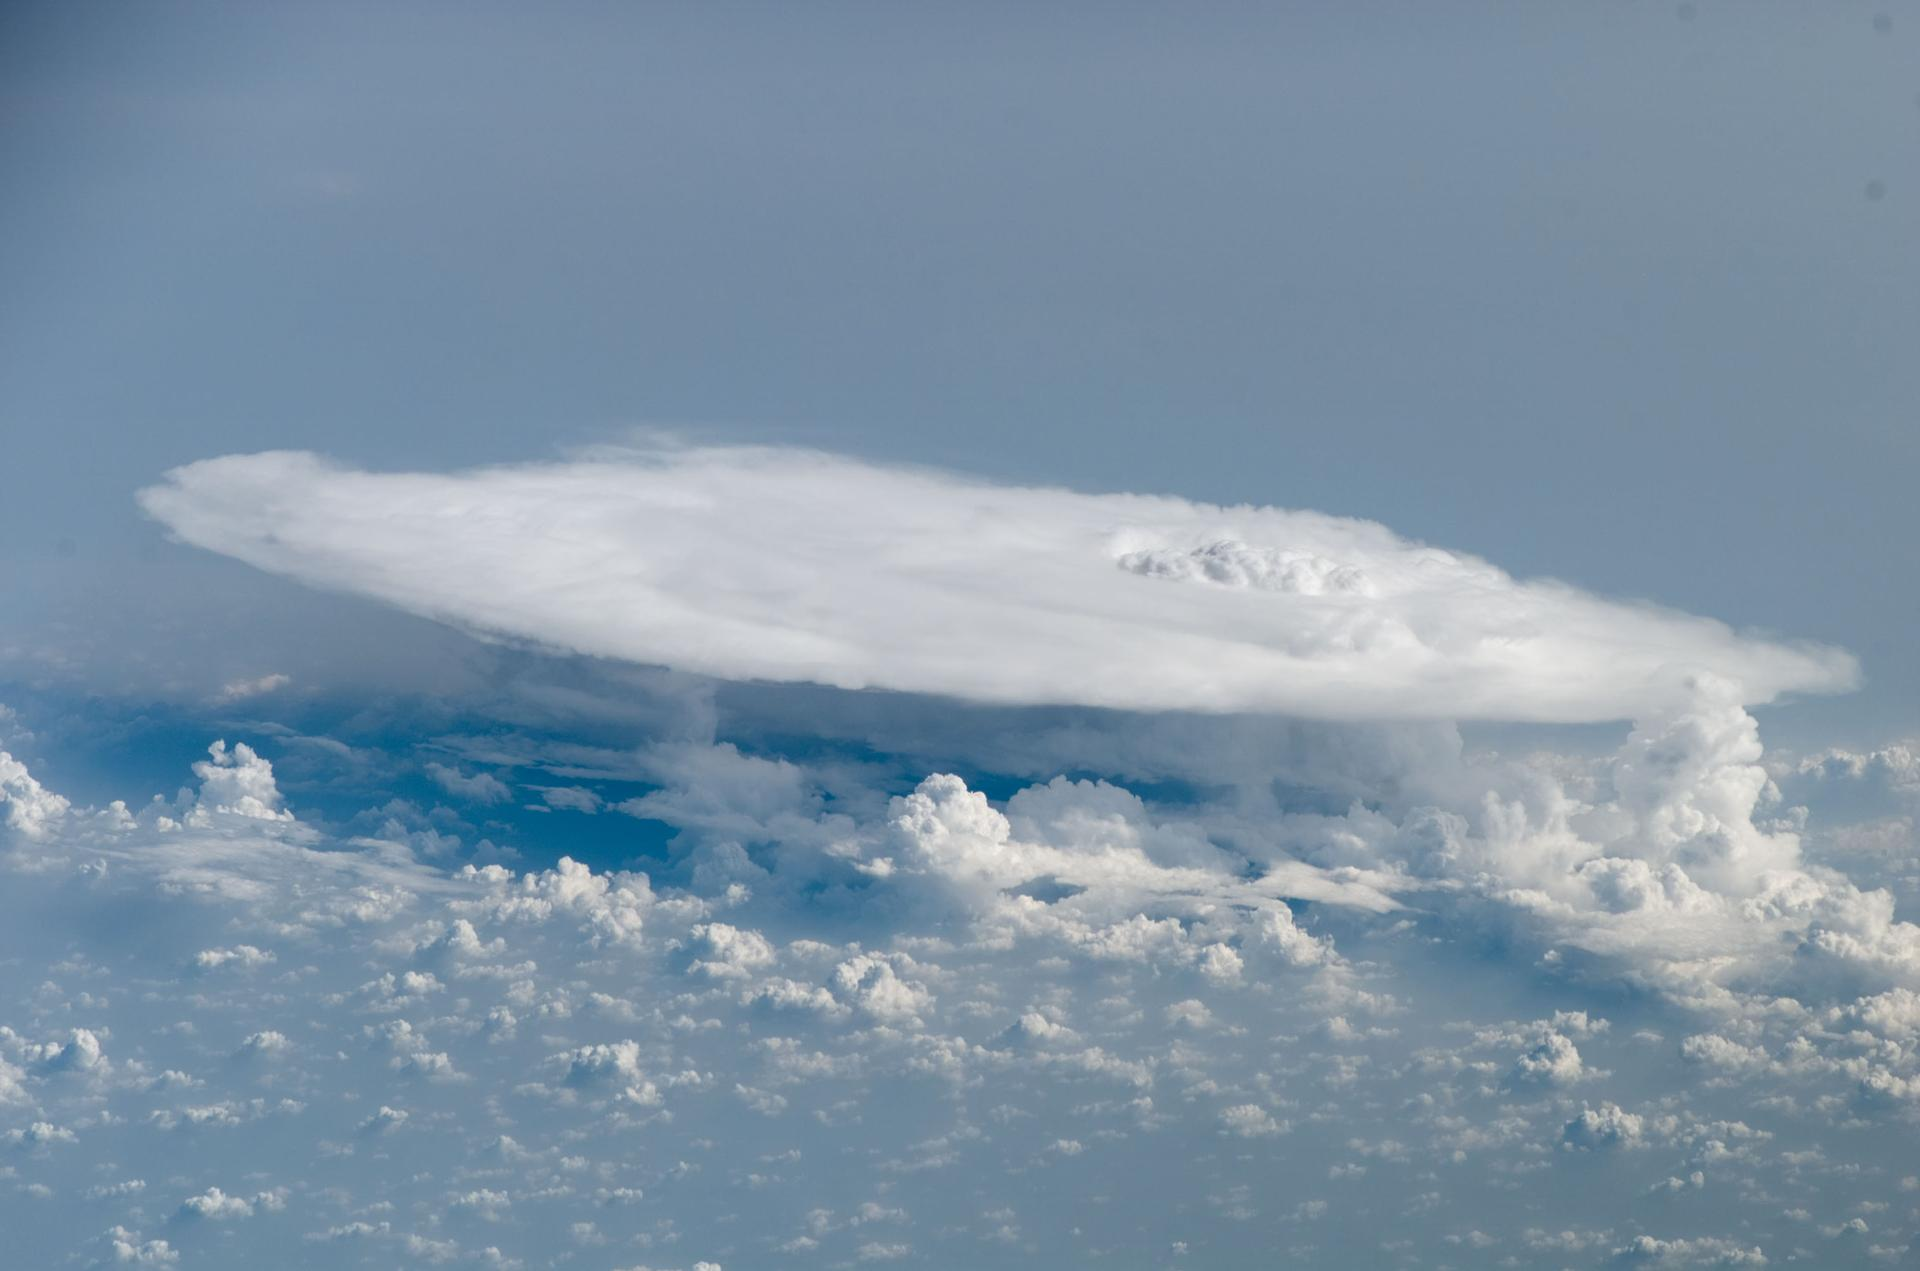
\includegraphics[width=\textwidth]{figures/cumulonimbus_nasa.jpg}
    \caption[
    A photograph of a \acrshort{dcc} seen over Africa from the ISS
    ]{
    A photograph of a \acrshort{dcc} seen over Africa from the International Space Station on 5th February 2008. The main convective core can be seen in the centre of the image as the turbulent, textured region emerging through the wide, flat anvil that surrounds it. On the right-hand side of the image a new core can be seen developing that is about to make contact with the anvil of the original core. Image credit: \acrshort{nasa} Image and Video Library, iss016e027426.
    }
    \label{fig:cb_photo}
\end{figure}

First identified as a unique cloud type in the late 19\textsuperscript{th}~century by \citet{abercromby_identity_1887} and \citet{hildebrandsson_remarks_1887}, \acrshort{dcc}s have been a focus of scientific investigation ever since.
\acrshort{dcc}s are the source of many severe weather events \citep{matsudo_severe_2011, houze_chapter_2014} including heavy precipitation \citep{westra_future_2014}, lightning \citep{williams_radar_1992}, hail \citep{punge_hail_2016}, flooding, tornadoes and tropical cyclones.

\acrshort{dcc}s play an important role in weather and climate beyond extreme events.
In the tropics, deep convection forms the ascending branch of the Hadley cell \citep{riehl_heat_1958}, and in doing so begins the transport of energy through the atmosphere from the equator to the poles.
In many regions of the world, from tropical Africa to the Great Plains of North America, \acrshort{dcc}s provide the majority of precipitation \citep{feng_global_2021}.
The large anvil clouds of \acrshort{dcc}s have a mediating effect on the radiative heating of the climate, reflecting incoming sunlight and trapping outgoing longwave radiation in equal amounts \citep{ramanathan_cloud-radiative_1989, hartmann_effect_1992, hartmann_tropical_2016}.

\acrshort{dcc}s are expected to have multiple responses to climate change.
Increases in atmospheric temperature and humidity increase both the intensity and frequency of heavy precipitation from deep convection \citep[e.g.][]{allen_constraints_2002, trenberth_changing_2003, held_robust_2006}.
In addition, global warming is also expected to lead to multiple radiative feedbacks from convective anvil clouds with both positive (warming) and negative (cooling) impacts \citep{bony_clouds_2015}.
These feedbacks remain one of the largest uncertainties in future climate projections \citep{sherwood_assessment_2020}.
Understanding the behaviour, interactions and feedbacks of \acrshort{dcc}s is therefore vital for understanding both our present-day climate and its response in a changing world \citep{gasparini_opinion_2023}.

Anthropogenic aerosols also affect \acrshort{dcc}s through aerosol--cloud interactions such as convective invigoration \citep{khain2005aerosol, rosenfeld_flood_2008}, although these processes remain uncertain \citep{varble_opinion_2023}.
Aerosol impacts on \acrshort{dcc}s are difficult to study in observations due to the small magnitude of the effects in comparison to meteorological variability and measurement uncertainty \citep{grabowski_can_2018}, as well as the difficulty in separating aerosol--cloud interactions from confounding processes \citep{varble_erroneous_2018}.
As a result, the effects of aerosols on \acrshort{dcc}s are not considered within the scope of this thesis.

\acrshort{dcc}s occur over a wide range of scales, and this limits the sources of observations which can fully capture their behaviour.
The processes of individual \acrshort{dcc}s span a scale from single kilometres and minutes, to hundreds of km and multiple days for large, organised convective systems.
When considering the response of the global circulation and atmospheric energy balance, it may take multiple years of observations for an equilibrium state to be observed \citep{muller_energetic_2011}.
Geostationary weather satellites, such as the \acrfull{noaa} \acrfull{goes} series and the \acrfull{eumetsat} Meteosat series have provided imagery of \acrshort{dcc}s over many decades for monitoring and predicting the weather.
However, these instruments have not traditionally supported the accuracy required for scientific studies, and it is only with the latest generation that the capability of this imagery for studying the behaviour of deep convection is being fully realised.

The study of \acrshort{dcc}s is made difficult by their complex, dynamic behaviours.
Many techniques used to study more slowly varying or spatially uniform atmospheric phenomena (including other cloud types, such as stratus and cumulostratus regions) cannot fully capture the complexity of \acrshort{dcc}s.
Even snapshot observations, such as those made by polar-orbiting earth observation satellites, cannot fully characterise \acrshort{dcc} behaviour, no matter how detailed they are, due to the rapid changes in the properties of \acrshort{dcc}s over their lifetimes.
Lagrangian methods---those which follow the \acrshort{dcc}s' motion---provide vital observations of \acrshort{dcc} properties over their lifecycle.
While particle trajectory models have been successfully utilised to study boundary layer clouds from a Lagrangian perspective \citep[e.g][]{eastman_competing_2018, christensen_aerosols_2020a}, these techniques are not easily applicable due to the complex wind environment of \acrshort{dcc}s, and the low accuracy of reanalysis models and derived \acrfullpl{amv} in these environments.
Instead, image processing methods that detect and track \acrshort{dcc}s are used to study their behaviour from a Lagrangian perspective.
These methods have seen a renaissance in recent years for studying deep convection, with applications including convective resolving models, weather radars and geostationary satellite imagery.
There remain several limitations in existing tracking models, and so the development of novel techniques is required to better understand the full spectrum of \acrshort{dcc}s.

Overall, understanding the behaviour of \acrshort{dcc}s and their response to climate change is vital both to predicting extreme weather events and climate feedbacks.
This introductory chapter will explore a range of topics regarding the behaviour of \acrshort{dcc}s and their further impacts.
In particular, it will focus on the relation between deep convection and the behaviour of anvil clouds, and how novel cloud tracking methods can be used to provide new insights from observations of \acrshort{dcc}s.


\section{Physical properties of \acrshort{dcc}s}

The physical nature of a \acrshort{dcc} can be divided into three parts: a cloud system, consisting of a multitude of liquid and ice water cloud particles along with several kinds of precipitation; a thermodynamic system in which moisture and energy are transformed into intense vertical motion and circulations across several scales; and a radiative system in which the large anvil reflects sunlight and absorbs \acrshort{lw} radiation, both heating and cooling the atmosphere within and below it.
These processes are not independent and interact with each other in numerous ways.
As a result, understanding each of them is important to understanding the behaviour of \acrshort{dcc}s.


\subsection{Cloud microphysical properties}

\acrshort{dcc}s, like any other cloud, are formed from a great number of water and ice particles suspended in the atmosphere.
\acrshort{dcc}s consist of a vertically growing core spanning from the \acrfull{pbl} to the tropopause, a distance often exceeding 10\,\unit{km}, with a diameter of ~10\,\unit{km} and updraught velocities of around 10\,\unit{ms\textsuperscript{-1}} \citep{weisman_mesoscale_2015}, and a surrounding anvil cloud formed due to horizontal divergence of cloud ice which has been lifted to the level of neutral buoyancy \citep{houze_chapter_2014}.
While the anvil cirrus of a \acrshort{dcc} consists of ice particles, many of these particles form in the liquid phase within the core, before freezing as they are lifted vertically and then detrained horizontally.
As a result, while ice--phase microphysics determines the evolution of anvil cirrus over time, liquid--phase microphysics are also important in \acrshort{dcc}s due to the initial formation of many anvil particles by homogeneous freezing of liquid droplets formed in the convective core.

% \begin{equation}
%     \frac{1}{e_s}\frac{d e_s}{dT} \cong \frac{L}{R_v T^2}
%     % \caption{The Clausius--Clapeyron relation for saturation vapour pressure}
% \end{equation}

\begin{eqfloat}
    \captionsetup{labelformat=empty}
    \caption{
    The Clausius--Clapeyron relation for saturation vapour pressure (eq.~\ref{eq:cc_rel}), where $e_s$ is the saturation vapour pressure, $T$ is the parcel temperature in Kelvin, $L_\mathrm{v}(T, p)$ is the latent heat of vaporisation of water, and $R_\mathrm{v}$ is the gas constant of water vapour. This cannot be solved analytically due to the temperature dependence of the latent heat of vaporisation. An accurate approximation in the form of the August--Roche--Magnus equation \citep{magnus_versuche_1844} be found empirically (eq.~\ref{eq:cc_rel_approx}, with coefficients from \citet{alduchov_improved_1997}).
    Similarly, the relation for saturation vapour pressure over ice ($e_\mathrm{s,i}$) is given by eq.~\ref{eq:cc_ice_rel}, where $L_\mathrm{s}(T,P)$ is the latent heat of sublimation of water (equivalent to $L_\mathrm{v} + L_\mathrm{f}$, the latent heat of fusion). 
    The empirical approximation for $e_\mathrm{s,i}$ is given by eq.~\ref{eq:cc_ice_rel_approx}.
    Note that at 0\,\textdegree C, $e_\mathrm{s,i} = e_\mathrm{s}$, whereas the the approximations differ slightly.
    }
    
    \begin{equation} 
    \label{eq:cc_rel}
        \frac{1}{e_{\mathrm{s}}}\frac{\mathrm{d} e_{\mathrm{s}}}{\mathrm{d} T} = \frac{L_\mathrm{v}(T, p)}{R_\mathrm{v} T^2}
    \end{equation}
    
    \begin{equation}
    \label{eq:cc_rel_approx}
        e_\mathrm{s}\left ( T \right ) \cong 6.1094\ \mathrm{kPa} \left ( \frac{17.625\ \mathrm{K}^{-1} \cdot (T - 273.15\ \mathrm{K})}{T - 30.11\ \mathrm{K}} \right )
    \end{equation}

    \begin{equation} 
    \label{eq:cc_ice_rel}
        \frac{1}{e_\mathrm{s,i}}\frac{\mathrm{d} e_{\mathrm{s,i}}}{\mathrm{d} T} = \frac{L_\mathrm{s}(T, p)}{R_\mathrm{v} T^2}
    \end{equation}
    
    \begin{equation}
    \label{eq:cc_ice_rel_approx}
        e_\mathrm{s,i}\left ( T \right ) \cong 6.1121\ \mathrm{kPa} \left ( \frac{22.587\ \mathrm{K}^{-1} \cdot (T - 273.15\ \mathrm{K})}{T + 0.71\ \mathrm{K}} \right )
    \end{equation}
    
\end{eqfloat}

When an airmass containing water vapour is lifted it expands and cools.
In doing so, the saturation vapour pressure decreases---in accordance with the Clausius-Clapeyron relation (eq.~\ref{eq:cc_rel})---at a faster rate than the specific vapour pressure of the airmass.
When the vapour pressure of the airmass exceeds the saturation vapour pressure it is considered supersaturated, and can condense to form cloud droplets.
It is very difficult for water droplets to form in a perfectly clean atmosphere, since for this to happen supersaturation of several hundred percent would be required.
Instead, soluble aerosol particles in the supersaturated airmass become the surface on which cloud droplets form, a process known as \acrfull{ccn} activation \citep{acci}.
The conditions under which aerosols can be activated as \acrshort{ccn} are given by the K{\"o}hler curves, which combine the competing effects of Kelvin's equation and Raoult's law on the equilibrium vapour pressure above the surface of a droplet. 
Kelvin's equation defines how the equilibrium vapour pressure increases as the radius of curvature decreases, therefore requiring a higher supersaturation for the activation of smaller droplets. 
Raoult's law regards the effect of soluble ions on the equilibrium vapour pressure: a larger amount of solute within the droplet reduces the required supersaturation. The resulting curve has a peak supersaturation requirement at a certain droplet radius. 
For an aerosol particle to be activated and grow into a cloud droplet it must either be larger than this radius and large enough that water can condense on it at the current supersaturation, or contain enough soluble ions that the peak supersaturation of the K{\"o}hler curve is less than the airmass supersaturation.
As a result, aerosol particles with high solubility---including in particular sulphate and nitrate aerosols, volatile organic compounds and sea salt---form the majority of \acrshort{ccn}.

Activated cloud droplets grow through two processes: condensation and coalescence. 
Condensation growth is most effective on small droplets, as they have the largest surface area to volume ratio, and is responsible for the growth of cloud droplets from the radius of \acrshort{ccn} (on the order of 0.1\,\unit{\mu m}) to that of a typical cloud droplet of around 10\,\unit{\mu m} \citep{cloud_physics}. 
This process also results in a narrowing of the cloud droplet size distribution. 
Coalescence growth occurs through either the merging of cloud droplets due to collision, or the collection of cloud droplets by rain droplets as the fall (accretion).
It becomes effective for larger cloud droplets beginning with radii of around 15\,\unit{\mu m} and is responsible for their growth into rain droplets \citep{cloud_physics}.
However, growth through condensation is very slow to reach the droplet sizes required for coalescence growth, and instead turbulence and the activation of giant \acrshort{ccn} \citep{feingold_impact_1999} are required for rain droplets to form.
On average, only about 30\% of the condensed water within a cloud will become rain droplets \citep{trenberth_changing_2003}, and the number of raindrops constitute a tiny fraction of the total number of droplets.

Ice clouds have important and complex microphysics.
Ice cloud particles may be formed either through direct deposition of water vapour into ice, or through the freezing of liquid cloud droplets.
Liquid water will not, however, freeze immediately below the freezing point due to the freezing energy barrier \citep{heymsfield_homogeneous_1993}.
Instead, liquid cloud droplets may exist in a super-cooled state, which may be frozen by one of two processes.
Homogeneous freezing occurs at temperatures below --38\,\textdegree C, allowing liquid droplets to freeze without external interactions \citep{koop_water_2000}.
As a result, homogeneous freezing of liquid cloud droplets tends to result in a larger number of smaller ice particles \citep{karcher_parameterization_2002, ickes_classical_2015}.
Heterogeneous freezing occurs due to the presence of \acrfullpl{inp} \citep{kanji_overview_2017a}.
\acrshort{inp}s reduce the freezing energy barrier due to having similar structures to ice crystals \citep{hoose_heterogeneous_2012}, and so allow freezing at warmer temperatures \citep{karcher_roles_2003}.
However, \acrshort{inp}s are somewhat rare in the atmosphere \citep{burrows_icenucleating_2022a}, and so heterogeneous freezing tends to result in fewer ice cloud particles, and, in some cases, mixed-phase clouds which consist of both ice and liquid droplets.

Ice particles may grow through deposition; the direct freezing of water vapour onto the surface of the crystal.
Similarly, ice crystals may lose mass due to sublimation, although due to the low rates of sublimation at cold temperatures this process is slow at high altitudes \citep{boehm_maintenance_1999, seeley_formation_2019}.
Ice crystals may grow through aggregation, where multiple crystals join together, or through riming, where super-cooled water droplets freeze on contact with an ice crystal \citep{ryan_growth_1976}.
In some conditions, additional, smaller ice crystals are produced through secondary ice production processes including rime-splintering \citep{hallett_production_1974}, droplet shattering and collision fragmentation \citep{field_secondary_2017a}.
These processes are common in deep convection due to strong updrafts, turbulence and the occurrence of homogeneous freezing, and so the most intense \acrshort{dcc}s tend to create anvils with smaller ice particles than those formed in in-situ cirrus.
Ice crystals are commonly removed from the atmosphere via sedimentation, which plays an important role in precipitation \citep{mulmenstadt_frequency_2015}.

Overall, ice cloud microphysics has complex dependencies on a wide range of factors.
In addition, these complex processes lead to a wide variety of shapes and sizes of ice particles, including both regular and irregular shapes \citep{waitz_situ_2022}, which adds further variance to ice crystal interactions.
The understanding of ice cloud microphysics, along with its parameterisations in climate models, is a large and important source of uncertainty in understanding clouds and future climate change \citep{sullivan_ice_2021, gasparini_opinion_2023}.


\subsection{Cloud radiative properties}

Cloud droplets interact with radiation both through the reflectance and scattering of solar visible and \acrfull{nir} radiation, and also through the absorbance and emission in the \acrshort{lw} spectrum.
While the reflection of incoming radiation has a cooling effect on the \acrfull{toa} atmospheric energy balance, the \acrshort{lw} effect of clouds is warming.
As a result, a cloud may have a net warming or cooling effect depending on the balance of these two factors.
The difference between the \acrshort{toa} radiative flux with clouds versus that for a clear sky is referred to as the \acrfull{cre}.

The \acrshort{sw} reflectance of a cloud depends upon both the microphysical properties of the cloud particles and the bulk properties of the cloud, including the number of droplets and the amount of liquid or ice.
The optical properties of a cloud are generally measured by two variables: the \acrfull{re} and the cloud optical thickness ($\tau$).
\acrshort{re} is the ratio of the third and second moments of the particle size distribution, which provides a good approximation of the mean scattering radius within a volume of cloud particles as long as the radius is larger than the wavelength (which, for cloud particles that tend to reflect mostly at shorter wavelengths, is almost always the case) \citep{hansen_light_1974}. 
While this is relatively straightforward for liquid cloud droplets, for ice clouds this is complicated by their non-spherical geometries \citep{wyser_effective_1998}.
$\tau$ is the negative logarithm of the transmittance through a cloud layer, and clouds with high optical thickness reflect more \acrshort{sw} radiation.
While $\tau$ varies with wavelength, it is mostly uniform throughout the visible wavelengths for cloud droplets \citep{hu_accurate_1993} and tends to be provided without a specified wavelength.
All values for $\tau$ provided in this thesis are taken at 550\,\unit{nm}, unless stated otherwise.
Due to the small variance of $\tau$ across the range of visible wavelengths, these values are considered directly comparable with those retrieved using geostationary satellite observations at 640\,\unit{nm}.

The \acrshort{lw} effect depends upon both the temperature (and hence height) of the cloud as well as their thickness and microphysics.
Clouds that are colder than the surface will emit less \acrshort{lw} radiation than they absorb and hence have a warming effect.
As the \acrshort{lw} absorption of clouds reduces more slowly as a cloud thins than their \acrshort{sw} reflectivity, thin clouds will tend to have a greater \acrshort{lw} effect than \acrshort{sw}.

Thick, low-level clouds, such as cumulus, stratocumulus and stratus have an overall cooling effect as they reflect a large proportion of incoming solar radiation but emit in the \acrshort{lw} at a similar temperature to the surface. 
On the contrary, high, thin, cirrus clouds have a strong warming effect as they transmit the majority of incoming solar radiation but emit at a much lower temperature than the surface. 
\acrshort{dcc} anvils, being both thick and at a high altitude, tend to have a balanced effect within 10\,\unit{Wm\textsuperscript{-2}} of neutral \citep{ramanathan_cloud-radiative_1989, hartmann_effect_1992, hartmann_tropical_2016}, however their \acrshort{sw} and \acrshort{lw} \acrshort{cre} both have large magnitudes. 
Overall, \acrshort{cre} has a cooling effect on the climate, but displays a positive feedback to global warming, generally attributed to a reduction in low, oceanic cloud coverage \citep{bony_clouds_2015}. 
This feedback is one of the largest uncertainties in future climate change \citep{sherwood_assessment_2020}, and recent research has found that this uncertainty may be underestimated by current \acrfullpl{gcm} \citep{hill_climate_2023}.
The feedbacks of \acrshort{dcc}s to climate change are particularly uncertain, and recent research has highlighted our lack of understanding of the response of the optical properties of \acrshort{dcc}s to increasing temperatures \citep{mckim_weak_2024}.
The response of \acrshort{dcc}s to climate change will be discussed in more detail in section~\ref{sec:anvil_feedbacks}.


\subsection{Thermodynamics of deep convection}

Deep convection requires three ingredients to occur \citep{brooks_century_2019}:. 
First, a build-up of conditional instability throughout the troposphere. 
Second, a source of moisture in the lower troposphere. 
Third, a buoyancy perturbation or vertical motion which lifts a parcel of moist, low-level air above the \acrfull{lcl} and the \acrfull{lfc}.

\begin{eqfloat}
    \begin{equation}
    \label{eq:full_bouyancy}
        B = g \left ( \frac{T - \bar{T}}{\bar{T}} + 0.61 \frac{q_\mathrm{v} - \bar{q}_\mathrm{v}}{\bar{q}_\mathrm{v}} - \frac{p - \bar{p}}{\bar{p}} - q_\mathrm{H} \right )
    \end{equation}
    \caption{The buoyancy equation for an air parcel perturbed from the surrounding environment. The buoyant acceleration, $B$, is approximately equal to gravitational acceleration times four terms, from left the right: the temperature term, the vapour term, where $q_\mathrm{v}$ is the mixing ratio of water vapour, the pressure perturbation term, and the hydrometeor drag, where $q_\mathrm{H}$ is the mixing ratio of hydrometeors. Variables with bars represent the background state.}
\end{eqfloat}

Conditional instability refers to a situation in which the decrease in temperature with height in an atmospheric column is greater than the moist pseudo-adiabatic lapse rate, but less than that of the dry adiabatic lapse rate. 
Whereas unconditional instability (where the temperature lapse rate is greater than the dry adiabatic lapse rate) is quickly stabilised through dry convection, conditional instability can continue to build until a convective cloud is formed. 
When water condenses, the latent heat released results in a positive buoyancy force (eq.~\ref{eq:full_bouyancy} which accelerates the parcel upwards leading to large vertical velocities.
The build-up of instability is measured as the \acrfull{cape} of an air parcel (eq.~\ref{eq:cape}), which represents the potential kinetic energy provided by the buoyancy of a parcel lifted above the \acrshort{lfc}. The work required to lift the parcel to the \acrshort{lfc} is measured as the \acrfull{cin} (eq.~\ref{eq:cin}). High values of \acrshort{cape} are associated with intense convection.

\begin{eqfloat}
    \begin{equation}
    \label{eq:simple_bouyancy}
        \frac{\mathrm{D} }{\mathrm{D} z} \left (\frac{w^2}{2}  \right ) = g \left ( \frac{T - \bar{T}}{\bar{T}} \right )
    \end{equation}
    \caption{By ignoring the pressure, vapour and hydrometeor terms of eq.~\ref{eq:full_bouyancy} the buoyancy equation can be written in terms of the vertical velocity, $w$, the height $z$ and temperature. \acrshort{cape} is calculated by integrating the right-hand side of the equation over height between the \acrshort{lfc} and the \acrfull{lnb} (eq.~\ref{eq:cape}). \acrshort{cin} is calculated by integrating the negative buoyancy between the initial position of the parcel and the \acrshort{lfc} (eq~\ref{eq:cin}).}
    \begin{equation}
    \label{eq:cape}
        \mathrm{CAPE} = g \int_{\mathrm{LFC}}^{\mathrm{LNB}} \left ( \frac{T - \bar{T}}{\bar{T}} \right ) \mathrm{d}z
    \end{equation}
    \begin{equation}
    \label{eq:cin}
        \mathrm{CIN} = - g \int_{z_0}^{\mathrm{LFC}} \left ( \frac{T - \bar{T}}{\bar{T}} \right ) \mathrm{d}z
    \end{equation}
\end{eqfloat}

The properties of a convective airmass are commonly derived using parcel theory \citep[][e.g.]{emanuel1983lagrangian}. 
This approach approximates the air parcel as undergoing adiabatic processes while it is lifted from the lower to the upper troposphere. 
The buoyancy of the air parcel along this trajectory is dependent on the initial height and moisture content of the parcel as well as the temperature profile of the environment it exists in. 
Analysis of these trajectories can be performed by plotting them on a thermodynamic diagram. 
An example of a tephigram, which plots the ascent of a parcel on axes of temperature and potential temperature which are skewed by 45 degrees, is shown in fig.~\ref{fig:parcel_ascent}.
The tephigram has advantages over other thermodynamic diagrams commonly used in meteorology, such as the T--logP diagram, as its axes are orthogonal to each other and therefore thermodynamic properties such as \acrshort{cape} and \acrshort{cin} are accurately represented by their areas.

\begin{figure}[tp]
    \centering
    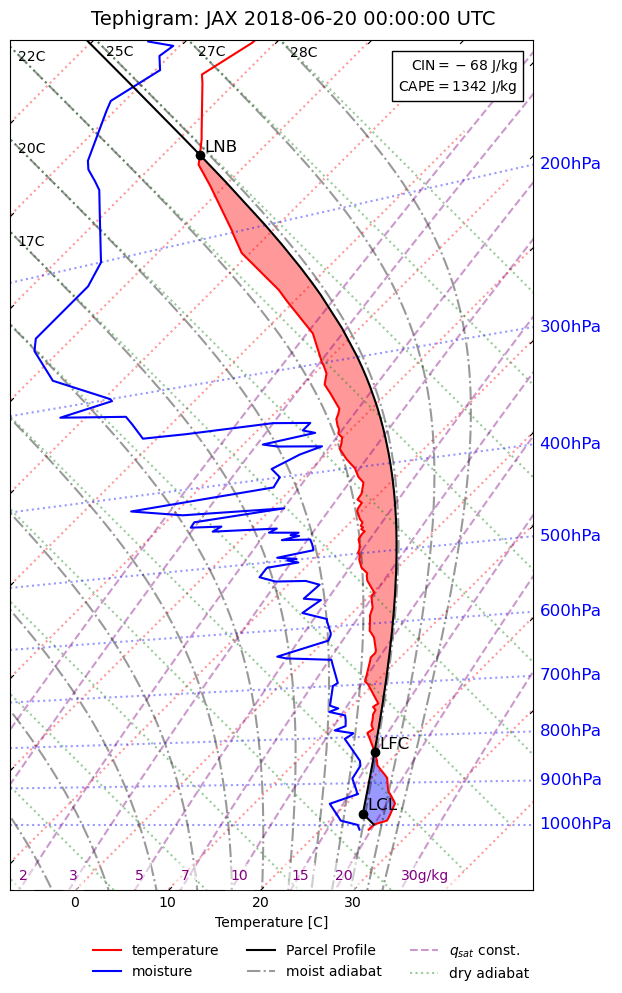
\includegraphics[width=0.75\textwidth]{figures/example_tephigram.png}
    \caption[
    An illustration of parcel ascent on a tephigram for a sounding taken on 2018-06-20 00:00 \acrshort{utc} at Jacksonville, Florida
    ]{
    An illustration of parcel ascent on a tephigram for a sounding taken on 2018-06-20 00:00 \acrshort{utc} at Jacksonville, Florida. The environmental temperature profile is shown by the red line, and the dewpoint temperature by the blue line. The path of the parcel, which starts near the surface, is shown by the black line. Points marking the \acrshort{lcl}, \acrshort{lfc} and \acrshort{lnb} are shown. The \acrshort{cape} and \acrshort{cin} are shown by the red and blue areas respectively.
    }
    \label{fig:parcel_ascent}
\end{figure}

From its initial position, the parcel is assumed to undergo adiabatic cooling as it is lifted until its temperature reaches that of the dew point of the initial airmass. 
At this point, the \acrshort{lcl}, the saturation of the airmass reaches 100\%, condensation occurs and the cloud begins to form. 
Beyond this point, the temperature of the parcel is assumed to follow the moist pseudo-adiabatic lapse rate. 
As this lapse rate is less than that of an environment with conditional instability, as the parcel continues to rise it will reach a point where its temperature is greater than that of the surrounding environment referred to as the \acrshort{lfc}. 
Above the \acrshort{lfc} the parcel will experience positive buoyancy. 
As the moist adiabatic lapse rate approaches that of the dry adiabatic lapse rate at low temperature and humidity (and hence at higher altitudes), and the environmental lapse rate reduces as it approaches the tropopause layer \citep{fueglistaler_tropical_2009}, the parcel will cool below the temperature of the surrounding environment. 
The point at which the temperature profile of the parcel again crosses that of the environment is called the \acrfull{lnb}. 
Although the air parcel may continue to rise above this point due to its momentum, negative buoyancy will act to halt its ascent.

Two further properties related to convection are also shown on the tephigram. 
\acrshort{cape} can be calculated as the area between the parcel temperature profile and the environment profile between the \acrshort{lfc} and the \acrshort{lnb}, showing clearly how \acrshort{cape} is the total work exerted by positive buoyancy forces between these two levels. 
From this, \acrshort{cape} can be used to calculate the theoretical maximum updraft velocity if all \acrshort{cape} is converted to kinetic energy, although typical maximum updraft velocities are half of this amount due to the dilution of updraft plumes through mixing with the surrounding environment \citep{lemone_cumulonimbus_1980, romps_undiluted_2010}. 
Similarly, \acrfull{cin} can be calculated as the area between the temperature profiles between the initial parcel location and the \acrshort{lfc}. 
\acrshort{cin} measures the work required to lift the parcel, overcoming negative buoyancy forces, in order to reach the \acrshort{lfc}.

There are a number of caveats with the parcel approach for deep convection that must be considered. 
The convective profile of a parcel depends upon its starting conditions including initial height, temperature and humidity. 
As a result, for even a single atmospheric column, a whole ensemble of parcels initialised at different locations within the PBL can be considered, each with different values of \acrshort{lcl}, \acrshort{lfc}, \acrshort{lnb}, \acrshort{cape} and \acrshort{cin}. 
To account for this, the mixed-layer \acrshort{cape} is often calculated from the average for parcels initiated in the \acrshort{pbl} \citep{stevens_atmospheric_2005}. 
In addition, the properties of the most unstable parcel may also be found in the same manner, which may provide useful information for predicting convective initiation.

Secondly, it is generally assumed that above the \acrshort{lcl} the parcel follows the moist pseudo-adiabat, which approximates that all condensed water is removed from the parcel immediately via precipitation \citep{emanuel_atmospheric_1994}. 
Although this approximation may seem to agree with the high precipitation rates of \acrshort{dcc}s, observed profiles of convective updrafts more closely match the moist adiabatic lapse rate (which assumes that all condensed water remains within the parcel) \citep{xu_is_1989}. 
In addition, while it is often considered that MSE is conserved in convective processes this is only correct in the case of environments in hydrostatic balance \citep{peters_evaluating_2021}. 
In deep convection, where this is not the case, it is a better approximation that MSE minus \acrshort{cape} is conserved \citep{romps_mse_2015}.

Finally, and arguably most importantly, is that the parcel model assumes that there is no mixing between the air parcel and the surrounding environment, a state that is referred to as undiluted. 
In the dynamic and turbulent environment of deep convection mixing does occur, however, and it is very rare for an undiluted state to occur \citep{zipser_cumulonimbus_1980, romps_undiluted_2010}. 
The entrainment of dry air into convective updrafts due to mixing reduces both \acrshort{cape} \citep{zhang_effects_2009} and the \acrshort{lnb} \citep{masunaga_convective_2016} as it adjusts the parcel profile closer to the background temperature profile, reducing the buoyancy forces. 
Observations of \acrshort{dcc}s have shown that while the highest cloud tops of \acrshort{dcc}s reach or even exceed the \acrshort{lnb}, the majority of the anvil cloud is detrained at a level substantially below the \acrshort{lnb} \citep{takahashi_where_2012, takahashi_level_2017}.

An additional factor not considered by the parcel model is the impact of circulation on instability.
Low-level convergence may transport additional heat and moisture to the base of the profile, increasing the potential for convection.
Wind shear---change in the speed and/or direction of wind with height---may also increase instability by transporting a colder airmass over a warmer boundary layer.
Wind shear plays an important role in the behaviour of \acrshort{dcc}s which will be explored in the following section.


\subsection{Lifecycle and structure of \acrshort{dcc}s}

The lifecycle of deep convection begins with the development of instability throughout the troposphere. 
The primary driver of instability is cooling through \acrshort{lw} emissions from water vapour, which cools the troposphere at around 2\,\unit{K} per day \citep{mapes_water_2001, jeevanjee_simple_2020}. 
\acrshort{sw} heating also affects instability which leads to diurnal differences which show large land--sea contrasts. 
Over land, \acrshort{sw} absorption warms the surface during the daytime, which sensible heating transfers to the lower troposphere. 
This \acrshort{sw} heating leads to an increase in \acrshort{cape} throughout the day, and, in particular, a peak in convective initiation in the afternoon due to surface heating and the resulting enthalpy flux into the \acrshort{pbl} \citep{hendon_diurnal_1993}.
On the contrary, over the ocean, \acrshort{sw} heating has less of an effect on the surface due to the greater heat capacity of water and the ocean mixed layer. 
Instead, a peak in instability is seen during the night and early morning \citep{gray_diurnal_1977}, which is believed to be due to the effects of \acrshort{sw} heating on the mid and upper troposphere during the day \citep{wall_life_2018}. 
The diurnal cycle of convection is much less pronounced over the ocean than over land \citep{soden_diurnal_2000}.
Instability can also be driven by the relative motion of air masses. 
Over the great plains of North America, warm, moist air is transported northward from the Gulf of Mexico which leads to instability as it moves under colder air \citep{walters_airflow_2001}.

Once sufficient instability has built up throughout the troposphere for deep convection to occur, a lifting action or buoyancy perturbation must occur to overcome \acrshort{cin} and initiate the formation of a \acrshort{dcc}.
This initiating process is referred to as the `triggering' of convection.
Triggering can occur through perturbations of the first three terms in the buoyancy equation (eq.~\ref{eq:full_bouyancy}).
\acrshort{sw} heating of the surface can cause an increase in surface air temperature through sensible heat fluxes, leading to dry convection and convective initiation.
Surface heating also causes latent heat fluxes, increasing the enthalpy and moisture content of the boundary layer.
In addition, the convergence of air masses within the boundary layer can also increase buoyancy by convergences of moisture and positive pressure perturbations.
Mechanical lifting mechanisms may also be involved in the initiation of convection.
Orographic lifting can occur when warm, moist air is blown towards mountains and cools as it ascends \citep{hodges_distribution_1997}. 
Gust fronts of cold, dense air may also act to lift warmer, moist air masses above them. 
These gust fronts may be caused by several processes, including synoptic frontal systems \citep{wilson_initiation_1986, jirak_observational_2007}, sea breeze \citep{tripoli_numerical_1979, park_environmental_2020}, and cold pools caused by precipitation \citep{grant_cold_2016}.

The occurrence of cumulus and cumulus congestus clouds (convective clouds in the low- and mid-troposphere \citep{johnson_trimodal_1999}) may also lead to deep convection. 
These lower-level convective clouds cause convergences of warm, moist air near the surface, building instability, and may also act to `condition’ the lower troposphere to convection by adjusting the environmental temperature profile closer to that of an ascending air parcel and hence reducing \acrshort{cin} \citep{masunaga_mechanism_2014, schulz_observing_2018}.

\begin{figure}[tp]
    \centering
    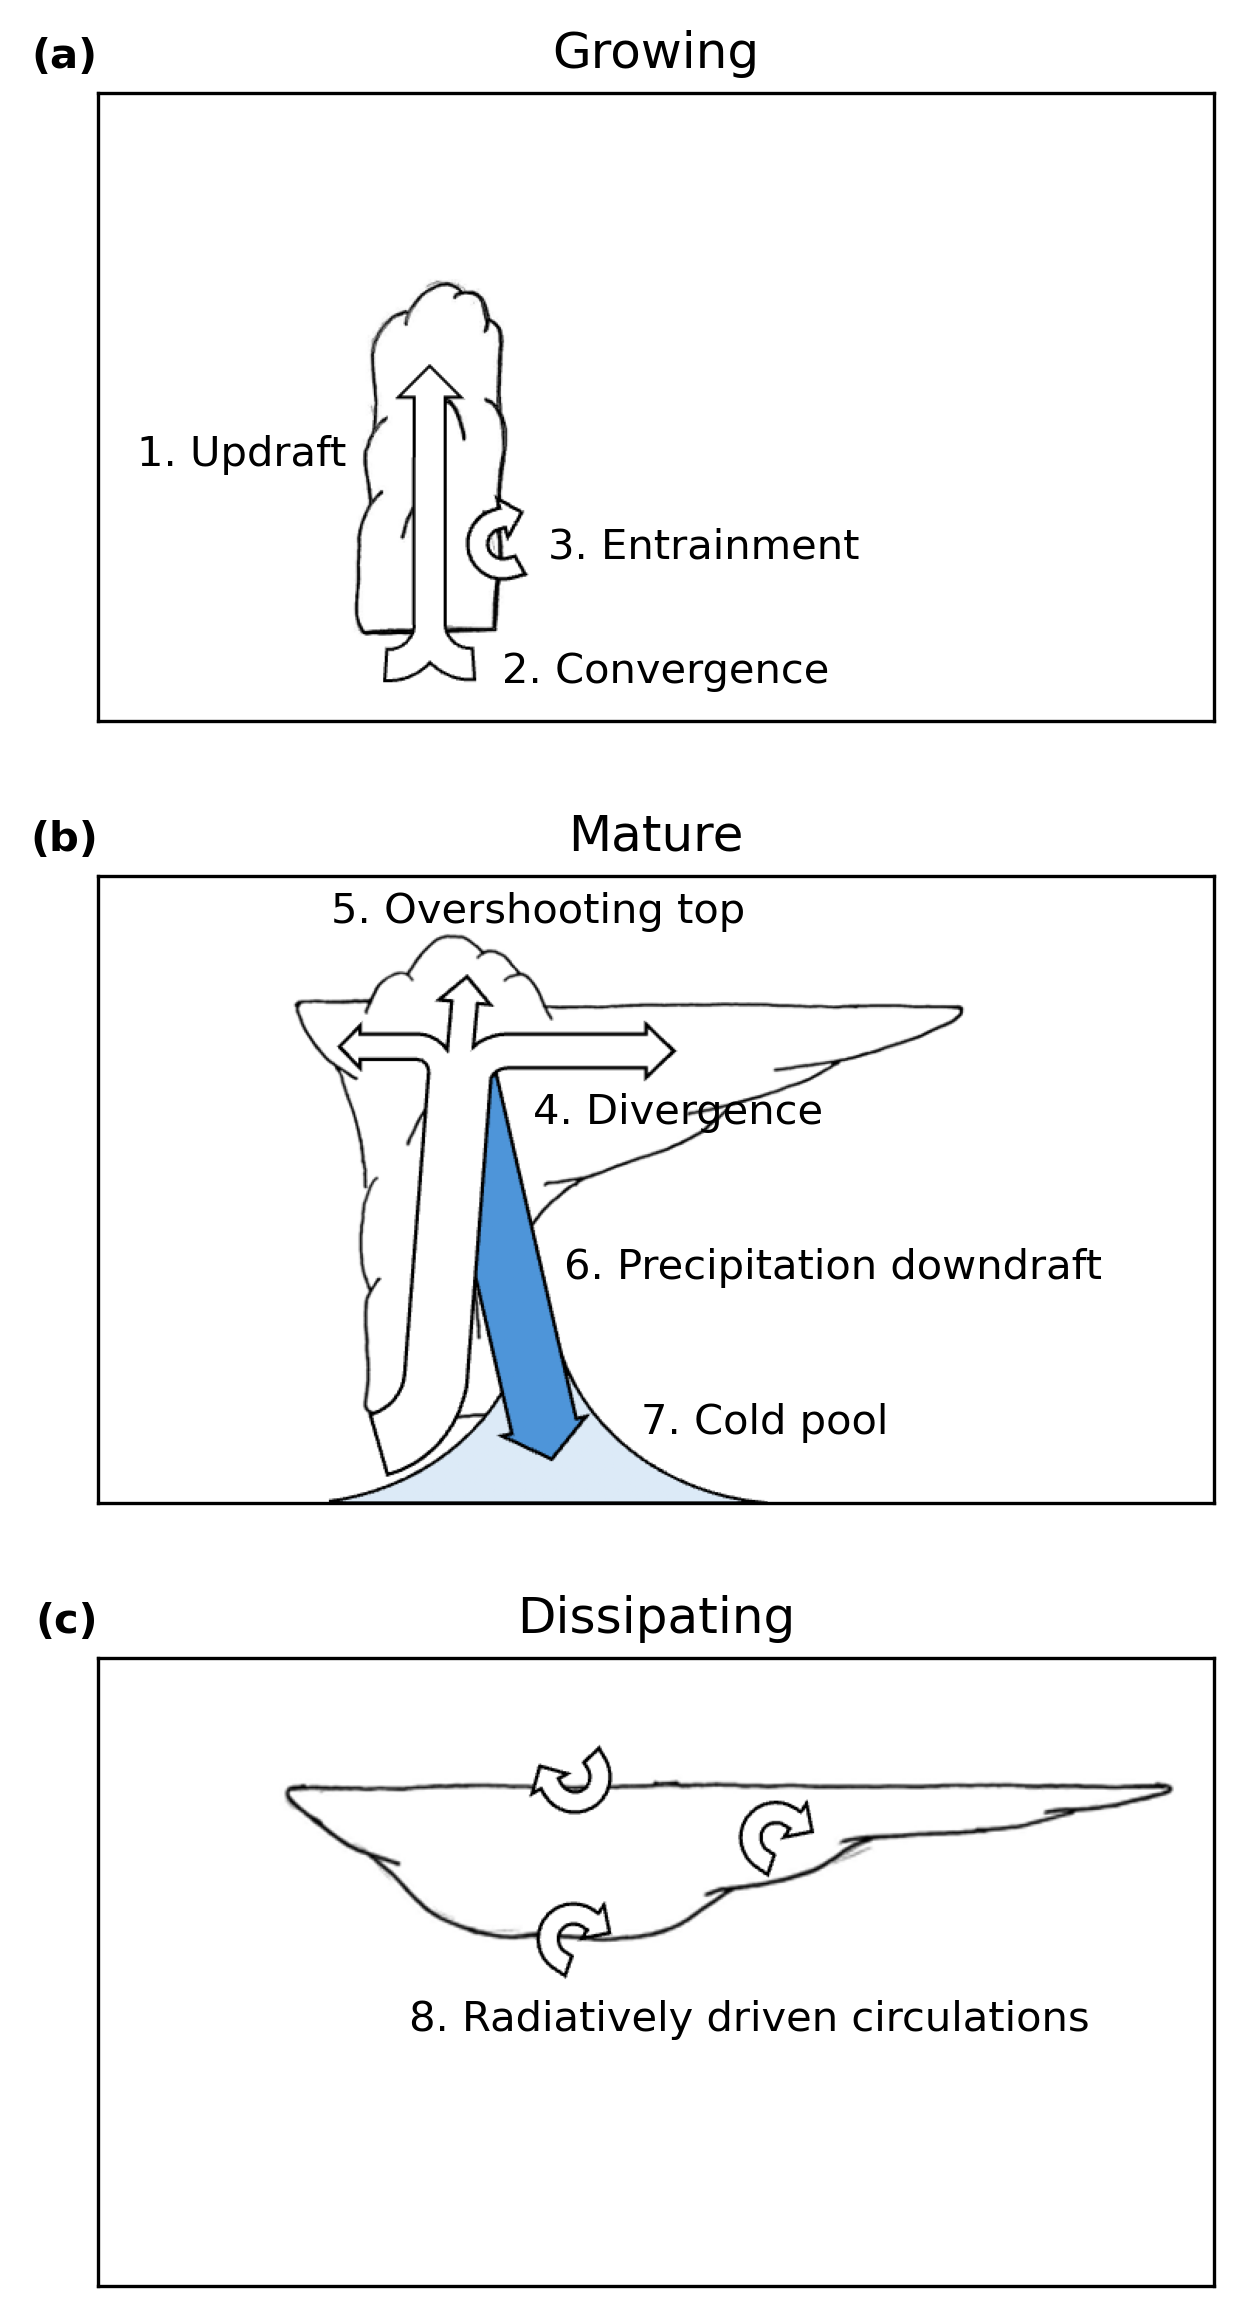
\includegraphics[width=0.5\textwidth]{figures/Intro_DCC_lifecycle.png}
    \caption[
    An illustration of the three lifecycle phases of an isolated \acrshort{dcc}
    ]{
    An illustration of the three lifecycle phases of an isolated \acrshort{dcc}: the growing (a), mature (b) and dissipating (c) phases. In the growing phase, the formation of a convective updraft (1) through positive buoyancy and convergence of warm, moist air at the cloud base (2) leads to a convective core that rapidly increases in height. Turbulent mixing with the surrounding environment (3) dilutes the updraft, reducing the buoyancy and hence vertical velocity. In the mature phase, the updraft reaches its \acrshort{lnb} resulting in divergence (4) and the formation of an anvil cloud. The momentum of the updraft within the core may result in it reaching the stratosphere, leading to an overshooting top (5). The onset of precipitation leads to downdrafts (6) due to hydrometeor drag and evaporative cooling, compensation for the downdraft. At the surface, this causes cold pools (7) which disrupt the inflow of air to the base of the storm, preventing further convective activity. In the dissipating phase there are no more convective dynamics, but radiative driven circulations (8) act to thin the thicker anvils due to entrainment of surrounding dry air, but increase the lifetime of thinner anvils.
    }
    \label{fig:dcc_lifecycle_illustration}
\end{figure}

Once initiated, the lifecycle of \acrshort{dcc}s can be separated into three sections: a growing phase, where the core develops vertically (fig.~\ref{fig:dcc_lifecycle_illustration}\,a); a mature phase in which the anvil cloud develops horizontally while convection continues within the core (fig.~\ref{fig:dcc_lifecycle_illustration}\,b); and a dissipating phase in which the anvil cloud dissipates after convective activity ceases within the core (fig.~\ref{fig:dcc_lifecycle_illustration}\,c) \citep{wall_life_2018}.
For isolated \acrshort{dcc}s (those consisting of a single core) the overall lifecycle typically spans 1-3~hours \citep{chen_diurnal_1997}.
However, \acrshort{dcc}s may also form with multiple cores feeding a single anvil cloud \citep{roca_simple_2017}, and in these cases may span areas several orders of magnitude larger \citep{houze_mesoscale_2004}, and exist for 10-20~hours or longer \citep{chen_diurnal_1997}.

The initiation stage occurs between the point of initiation and the time at which the top of the convective core stops growing upwards.
During this stage precipitation may occur in both the warm and ice phases, and the horizontal growth of the cloud is small in comparison to the vertical growth.
The initiation stage can be further broken down into the periods before and after the onset of freezing.
Freezing releases additional latent heat of fusion, although this may not contribute additional buoyancy as it is compensated for by the environmental lapse rate \citep{seeley_tropical_2016}.

Due to the large vertical velocities and high supersaturation present in deep convective updrafts, freezing is dominated by homogeneous freezing processes.
Furthermore, the intense dynamics result in a high rate of secondary ice production through the collision of droplets and rime--splintering.
As a result, \acrshort{dcc}s tend to form with a large number of small ice particles.
In convective updrafts with large vertical velocity, the momentum of the growing cloud may propel it above the \acrshort{lnb}.
This produces a phenomenon known as an overshooting top, where the top of the core penetrates the tropopause and extends into the stratosphere despite experiencing negative buoyancy.
As the cloud will continue to cool adiabatically as they rise, the tops of these updrafts can reach substantially colder temperatures than the surrounding environment \citep{proud_recordlow_2021}.

The mature stage occurs after the top of the \acrshort{dcc} has reached the level of neutral buoyancy.
The heaviest rates of convective precipitation occur during this stage, and the anvil cloud is formed \citep{houze_chapter_2014}.
The occurrence of heavy precipitation suppresses the convective core both through the generation of downdrafts and through the stabilisation effect of evaporating rain droplets.
This process will eventually weaken and dissipate the convective core of the \acrshort{dcc} unless the wind shear is large enough to advect the convective rainfall away from the convective core.
Furthermore, the evaporation of falling precipitation leads to the divergence of cold, dense air near the surface.
These cold pools may suppress further convective activity, while their gust fronts can also trigger new convective initiations.

The final stage of the \acrshort{dcc} lifecycle occurs after the convective core has dissipated and convective rainfall has stopped, and is referred to as the dissipating phase.
During this phase, the anvil cloud may continue to expand, with maximum anvil cloud extent occurring much later than maximum convective intensity \citep{futyan_deep_2007}.
Additional, stratiform, precipitation may occur throughout the anvil cloud, but this will not be as intense as the earlier convective precipitation \citep{houze_chapter_2014}.
The dissipating stage may also be split into two separate periods; those before and after the end of stratiform precipitation \citep{wall_life_2018}.

\acrshort{dcc}s can also be categorised spatially into three components.
Firstly, the core region, in which the convective updraught and convective precipitation occur.
Secondly, the anvil or cloud shield, which consists of a large area of thick cloud surrounding the core at the level of neutral buoyancy, and within which stratiform precipitation may occur.
Finally, the area of cirrus outflow, where thin ice cloud extends beyond the edge of the anvil cloud, particularly within the dissipating phase \citep{lilly_cirrus_1988}.
This structure of an isolated \acrshort{dcc} is also referred to as a `hot tower' \citep{riehl_northeast_1951}.

Radiative heating of the anvil cloud base and cooling of the anvil cloud top causes two regions of instability to occur. 
These unstable profiles drive circulations at the cloud base and top which increase the entrainment of dry air into the anvil while also lifting the anvil higher in the troposphere. 
While SW heating during the daytime reduces the instability at the cloud top, the greater LW heating at the cloud base results in a greater net dissipation of anvil during the daytime \citep{sokol_tropical_2020}. 
As the anvil cloud thins, these two regions of instability join into a single lapse rate. 
This state drives circulations within the anvil cloud which lift ice particles, reducing sedimentation and increasing particle growth \citep{gasparini_opinion_2023}. 
These circulations prolong the lifetime of the thin anvil cloud \citep{sokol_tropical_2020}. 
Further thinning of the cirrus anvil results in uniform radiative heating throughout the anvil, ending the circulation and leading the to complete dissipation of the anvil cloud. 


\subsection{Convective organisation}

While the majority of \acrshort{dcc}s form as isolated storms, with a single convective core that detrains an anvil cloud separated from its neighbours \citep{riehl_northeast_1951}.
In other cases, \acrshort{dcc}s exist with multiple convective cores feeding a single anvil cloud \citep{zipser_role_1969, nakazawa_tropical_1988}.
At the largest end of this progression are \acrfullpl{mcs}, which occur when a cluster of deep convective cores form a single large area of anvil referred to as a cloud shield \citep{roca_simple_2017}.
These \acrshort{mcs} cloud shields can cover an area of greater than 10,000~km\textsuperscript{2}, several orders of magnitude greater than that of individual \acrshort{dcc}s \citep{houze_mesoscale_2004}.

The convective cores that form \acrshort{mcs}s do not group together randomly, but are instead clustered by a complex group of processes that are referred to as convective organisation.
In general, these processes tend to lead to the triggering of new convective cores that feed the same cloud shield, expanding and extending the life of the system as they do.
\acrshort{mcs}s occur in many shapes and sizes, including mesoscale convective complexes, squall lines and tropical cloud clusters \citep{tsakraklides_global_2003a} which each have unique properties.
However, all \acrshort{mcs}s display large-scale processes that initiate new convective updrafts, and increase the size and lifetime of the anvil.

The lifecycle of \acrshort{mcs}s can be described similarly to that of isolated \acrshort{dcc}s through the three-phase growing, mature, dissipating structure \citep{futyan_deep_2007}.
It should be kept in mind however that when applied to \acrshort{mcs}s, these lifecycle stages do not represent the changes in convective processes as described for isolated \acrshort{dcc}s, but the mesoscale development and decay of the entire system.
The lifetime of these systems is substantially lengthened, with typical \acrshort{mcs}s lasting for 10 to 20 hours or longer \citep{chen_diurnal_1997}.
In particular, there is an increase in the lengths of the initiation and mature phases compared to isolated \acrshort{dcc}s \citep{wall_life_2018} due to the continuous development of new cores throughout the active lifetime of the \acrshort{mcs}.
The total lifetime of \acrshort{mcs}s is determined by the rate at which new cores are triggered, and observations have shown that they tend to decay once the area of convective cores falls below 10\% of the total anvil area \citep{elsaesser_simple_2022}.

A key feature that distinguishes \acrshort{mcs}s from smaller \acrshort{dcc}s is the development of large, mesoscale circulations that occur on larger scales than that of individual convective cores.
As well as the convergence of heat and moisture at low levels due to the convective cores, this mesoscale circulation draws in additional air from the surrounding areas at the mid-levels of the atmosphere.
This mid-level air does not enter the cloud shield through the convective cores, but instead condenses at higher altitudes, leading to a top-heavy latent heating profile within the cloud shield \citep{schumacher_tropical_2004}.
These organised convective cloud systems have thermodynamic impacts on the environment to a much greater extent than isolated \acrshort{dcc}s.
The large cloud shields of the \acrshort{mcs} s result in much larger amounts of stratiform precipitation than individual \acrshort{dcc}s, which is distributed over a much wider area \citep{houze_chapter_2014}.
These organised convective cloud systems have thermodynamic impacts on the environment to a much greater extent than isolated \acrshort{dcc}s, with idealised simulations showing that the thermodynamic interactions of organised convective systems can propagate thousands of kilometres within the troposphere \citep{beucler_budget_2019}.
Over time, the mesoscale circulation results in a moistening of the convective system and a drying of the surrounding atmosphere, creating a sharp contrast between the two regions \citep{bretherton_energybalance_2005}.

\acrshort{mcs}s are also characterised by both high rates and large volumes of precipitation, providing the majority of precipitation throughout the tropics as well as in many other regions \citep{feng_global_2021}.
Unlike isolated \acrshort{dcc}s, much of the precipitation occurs not as convective rainfall, but as stratiform rain from the cloud shield \citep{schumacher_stratiform_2003}.
As much as 70\,\% of the total precipitation of an \acrshort{mcs} can come from the stratiform rain, with a higher proportion observed over the ocean than in \acrshort{mcs}s over land.
Much of this stratiform precipitation can be attributed to the mid-level, mesoscale inflow to the cloud shield as well as the top-heavy latent heating profile.

The processes through which \acrshort{mcs}s form in the first place are still uncertain, however \citep{houze_100_2018}.
Convective organisation processes have been observed in satellite remote sensing, radiative-convective equilibrium models and cloud-resolving models \citep{holloway_observing_2017}. 
The formation and lifetime of \acrshort{mcs}s are strongly linked to the dynamics of the surrounding environment through the convergence of moist, low-level air and the divergence of air at the top of the \acrshort{mcs}  \citep{houze_chapter_2014}. 
Cold pools have a strong influence on the organisation of convective cores, and set the scales over which organisation occurs \citep{jeevanjee_convective_2013}, as their gust fronts, transport of moisture and collisions are vital to triggering new convection within \acrshort{mcs}s \citep{feng_mechanisms_2015}.
\acrshort{mcs}s have a tendency to trigger additional convection around the storm, blurring the boundary between the \acrshort{mcs} and isolated convection \citep{mapes_gregarious_1993}.

\acrshort{mcs}s are, in general, poorly represented in large-scale climate models due to the inability of the parameterised convection to organise between grid squares \citep{houze_100_2018}.
While convective resolving models have been proposed as a solution to this issue \citep{stevens_added_2020}, these models still do not represent \acrshort{mcs}s accurately with a tendency towards too little organisation \citep{prein_sensitivity_2021}.
Gaining a better understanding of the properties and processes of \acrshort{mcs}, both in observations and models, is vital therefore for improving their representation \citep{feng_mesoscale_2023}.
Changes in convective organisation have important effects on the global climate, with increases in organisation correlated with domain-wide \acrshort{toa} cooling in satellite observations \citep{bony_observed_2020}, and so future changes in organisation may have a large influence on the equilibrium climate sensitivity.


\section{Anvil Radiative Feedbacks} \label{sec:anvil_feedbacks}

There are a number of hypotheses regarding the \acrshort{cre} of tropical anvil clouds that consider whether the neutral \acrshort{cre} of tropical anvils is the result of a feedback mechanism. 
\citet{ramanathan_cloud-radiative_1989} proposed the thermostat hypothesis in which, in response to a warming environment, anvil clouds produce thicker cirrus which acts to cool the tropics through increased \acrshort{sw} reflectance. 
The Iris hypothesis proposes that anvil cirrus will decrease in area, resulting in greater \acrshort{lw} emission from the surrounding clear-sky regions.
\citet{lindzen_does_2001} first proposed this as a result of increased precipitation efficiency, however evidence for this effect is disputed \citep{genio_climatic_2002, lin_examination_2004}.
\citet{bony_thermodynamic_2016} proposed a `stability iris' feedback, in which the established trends of increased dry static stability \citep{held_robust_2006} and a reduction in the tropical overturning circulation \citep{vecchi_global_2007} reduce the detrainment of anvil cirrus.
Although the anvil cloud response is generally considered to be a negative climate feedback, the predicted magnitude varies widely and it represents the greatest uncertainty among all cloud feedbacks \citep{sherwood_assessment_2020}.

On the other hand, the \acrfull{fat} hypothesis argues that the anvil \acrfull{ctt} remains constant in a warming climate, and the greater difference between anvil and surface temperatures result in a positive \acrshort{lw} feedback \citep{hartmann_important_2002}.
The basis for \acrfull{fat} is that \acrshort{lw} cooling of the troposphere due to water vapour becomes inefficient below 220\,\unit{K} \citep{jeevanjee_simple_2020}, which, if relative humidity remains constant, fixes the top of the convectively active troposphere at this isotherm. 
While there is evidence that this is the case for the largest \acrshort{dcc} anvils, the increase in static stability may result in a reduced positive feedback due to a `proportionally higher' anvil temperature \citep{zelinka_why_2010} which more closely matches the \acrshort{lw} response of tropical clouds in global climate models.
While satellite observations have shown a trend in anvil cloud height \citep{norris_evidence_2016}, there is not yet sufficient evidence to distinguish this from inter-annual variability \citep{takahashi_when_2019}.
\citet{seeley_fat_2019}, argued that \acrshort{fat} is a weak constraint on anvil temperature as while the radiative tropopause temperature remains fixed, the temperature of the tropopause lapse rate inversion can vary widely. 
Furthermore, as anvils tend to detrain below the tropopause, \citep{takahashi_level_2017, wang_observational_2020}, anvil temperature and the tropopause temperature may only be weakly connected.
\citet{seidel_temperatures_2022} however found the inclusion of CO\textsubscript{2} radiative heating produces anvil temperatures consistent with \acrshort{fat}.

While the iris and \acrshort{fat} feedbacks may act to cancel each other out, and hence maintain the neutral \acrshort{cre} of tropical anvil clouds, other important feedback mechanisms may influence this balance.
\citet{hill_climate_2023} recently showed that climate models underestimate dynamically driven cloud feedbacks including changes in convective intensity.
Furthermore, convective instability is expected to scale with temperature in the same manner as the Clausius-Clapeyron relation \citep{seeley_why_2015, agard_clausius_2017}, and some observations of tropical anvil clouds have instead suggested that warming of the surface invigorates convection \citep{igel_cloudsat_2014}.
This invigoration effect may result in colder anvil \acrfull{ctt}, and hence a stronger warming feedback.
Multi-decadal satellite observations have shown a cooling of upper tropospheric cloud temperature over land \citep{liu_observed_2023}, indicating that changes in convective processes may lead to stronger cooling feedbacks.

A recent criticism of the \citet{sherwood_assessment_2020} decomposition of anvil feedbacks into the area response and the height response is that, by ignoring changes in the optical properties and structure of anvil clouds, these feedbacks are merged into the calculated iris effect, increasing its uncertainty \citep{raghuraman_observational_2024}.
\citet{mckim_weak_2024} proposed that the anvil area feedback of --0.40\,\unit{W m\textsuperscript{-2} K\textsuperscript{-1}} from \citet{sherwood_assessment_2020} would require an unrealistic anvil area change of --20\,\unit{\% K\textsuperscript{-1}}, indicating that there are other mechanisms contributing to the measured change in anvil \acrshort{cre}.
Recent work has proposed that the anvil cloud response reduces the area of thicker anvils with high \acrshort{iwc}, but not thinner cirrus, resulting in a much smaller overall feedback \citep{mckim_weak_2024, sokol_greater_2024}.

Changes to the lifecycle and diurnal cycle of deep convection may also be an important factor, particularly when considering the \acrshort{sw} feedback. 
\citet{nowicki_observations_2004} used estimates of \acrfull{toa} \acrshort{lw} and \acrshort{sw} radiative fluxes from \acrfull{seviri} observations to estimate the diurnal cycle of anvil \acrshort{cre} over equatorial Africa and the equatorial Atlantic. 
They found that shifting the diurnal cycle of deep convection in these regions could change the \acrshort{cre} by \textpm 10\,\unit{Wm\textsuperscript{-2}}, but did not track the properties of individual \acrshort{dcc}s.
\citet{bouniol_macrophysical_2016} compared \acrshort{cre} and cloud radiative heating rates to anvil cloud properties to investigate how radiative heating affects the anvil cloud evolution.
These observations were made with polar orbiting instruments however, and they highlighted the need for geostationary observations to characterise the evolution of individual anvil clouds.
Subsequent research used \acrshort{dcc} tracking methods to better characterise the lifecycle of observed anvil clouds \citep{bouniol_life_2021}, but as the radiative flux data was provided by polar-orbiting satellites the \acrshort{cre} could not be measured over the lifetime of the \acrshort{dcc}.


\section{Detection and tracking of deep convection} \label{sec:tracking_timeline}

The detection and tracking of clouds has been performed since the earliest sequences of remote sensing imagery from weather radar and geostationary satellites \citep{menzel_cloud_2001}.
\citet{fujita_study_1968} compared sequences of images observed by the first geostationary weather satellite to those taken using an all-sky camera, and found that by comparing subsequent observations from the satellite one could calculate \acrshort{amv}s similar to those observed on the ground.
This tracking of cloud position was performed by hand, and subsequently a plastic stencil `computer' was designed to calculate cloud velocities taking into account the satellite viewing geometry \citep{fujita_present_1969}.
While these early methods compared print-outs of satellite imagery by hand, shortly after a digital computer system was developed to show sequences of images \citep{chang_metracom_1973}.
Although detection and tracking were still performed manually (albeit with the user selecting cloud positions in subsequent images using the cursor), velocity calculation was performed automatically.
Wider adoption of this technology was applied to produce \acrshort{amv}s during field campaigns in the mid- to late-1970s \citep{tecson_cloud-motion_1975}.

There was, however, concern regarding the manual tracking of cloud velocity.
This task was both time consuming and also open to subjective judgement which made uncertainties hard to estimate.
\citet{fujita_satellite-tracked_1975} found large variations in \acrshort{amv}s produced using these methods.
Early efforts at automation applied cross-correlation techniques, previously used with weather radar, to estimate \acrshort{amv}s in geostationary satellite imagery \citep{leese_determination_1970}.
\citet{endlich_use_1971} applied a pattern matching technique to `brightness centres' in visible satellite imagery to estimate cloud motion.
\citet{rinehart_three-dimensional_1978} produced a cross-correlation algorithm for the estimation of convective cell motion in 3-D weather radar observations.
While these automated methods provided more accurate motion estimates than humans, they were less capable of detecting independent cloud motions both due to errors introduced by noise, and also due to the visible imagery provided by early geostationary satellites meaning it was difficult to distinguish clouds at different altitudes.

Automatic methods for the detection and tracking of \acrshort{dcc}s were developed for both radar reflectivity \citep{crane_automatic_1979} and geostationary satellite \acrshort{lw} \acrfull{ir} \acrfull{bt} \citep{endlich_automatic_1981}.
Both of these methods detected \acrshort{dcc} features by labelling the area surrounding local extrema (maxima for radar reflectivity, minima for \acrshort{bt}) in individual images.
The addition of 11\,\unit{\mu m} \acrshort{ir}-window \acrshort{bt} channels to the first operational \acrshort{goes} and Meteosat weather satellites allowed \acrshort{dcc}s to be distinguished from low clouds.
The centroids (the location of the feature represented as a single point) of these detected features were then linked to create \acrshort{dcc} tracks through the use of cost-minimisation algorithms with sought to find the best match between pairs of features detected at subsequent time steps.
By explicitly detecting features to track, these algorithms both improved upon the weakness of previous algorithms, but also allowed the properties of tracked objects to be studied beyond their motion vectors.

The development of \acrshort{dcc} detection and tracking algorithms continued in parallel for both radar and satellite observations.
\citet{rosenfeld_objective_1987} and \citet{williams_satellite-observed_1987} both developed overlap tracking techniques for radar reflectivity and satellite \acrshort{bt} observations respectively.
Unlike the prior centroid-based tracking methods, these overlap methods took into account the spatial extent of detected features by linking subsequent pairs of features based on those which shared the largest overlapping area.
By removing the approximation of a point-like feature, the overlap techniques better handle cases of \acrshort{dcc}s with larger, more complex shapes.
The downside to this approach, however, is that, unless the spatial extent of the \acrshort{dcc} is propagated using an estimate of the storm motion, it requires that the detected features do not move further than their diameter between subsequent observations.
As a result, for small, fast-moving objects (such as convective cells), or observations that are more widely spaced, overlap methods perform poorly.

Early detection and tracking algorithms were strongly limited by the available computational power which restricted tracking to only a small number of \acrshort{dcc}s. 
Furthermore, the accuracy of early algorithms was such that human verification of tracked objects was still required. 
The majority of algorithms were designed with only a single source of observations, which, in particular for weather radars, reduced the area over which tracking could be performed. 
While geostationary satellites provided larger areas of observations, the low spatial and temporal resolution of early sensors limited studies to large and long-lived \acrshort{mcs}s only. 
\citet{maddox_mesoscale_1980a} tracked mesoscale convective complexes over the US, and subsequent studies showed their distributions globally \citep{laing_global_1997}.

Subsequent development produced trends in both those algorithms used to track \acrshort{dcc}s in satellite imagery, and those using weather radar.
Algorithms using geostationary satellite imagery focused on the study of \acrshort{mcs}s, and tended to use overlap-based tracking methods \citep{arnaud_automatic_1992, evans_procedure_1996, carvalho_satellite_2001, morel_climatology_2002}.
On the other hand, tracking algorithms using radar reflectivity tended to focus on the tracking of convective cells, and favoured centroid-based tracking approaches \citep{dixon_titan_1993, johnson_storm_1998, handwerker_cell_2002}.
Across both sets of algorithms, the use of fixed thresholds rather than extrema for locating features became favoured due to the low computational cost, ease of customisation and resilience to noise \citep{augustine_mesoscale_1988}.
While the majority of approaches used a single threshold, some algorithms began using multiple thresholds to better characterise the detected features of \acrshort{dcc}s.
\citet{johnson_storm_1998} used a sequence of increasingly larger thresholds to better distinguish individual convective cells, and classify them according the intensity.
For \acrshort{mcs} detection, the `detect-and-spread' approach was used by \citet{evans_procedure_1996} and \citet{boer_lagrangian_1997} to better measure the area of \acrshort{mcs}s by first detecting the `core' using a cold \acrshort{bt} threshold and then detecting the surrounding cloud area using a warmer threshold.
It should be noted however that \citet{augustine_mesoscale_1988} argued that the area estimated using the warmer threshold is highly subjective.

\citet{hodges_general_1994} developed a more general algorithm for use with multiple gridded datasets, including model data, and subsequently expanded this approach to consider detection and tracking on a sphere for use with \acrshort{gcm}s \citep{hodges_feature_1995}.
The low spatial and temporal resolution of \acrshort{gcm}s of the time however meant that detection and tracking of individual \acrshort{dcc}s was not possible.
Other data, such as rainfall measurements and lightning flash observations, were also used to develop detection and tracking algorithms \citep{steinacker_automatic_2000}, however the vast majority of algorithms continued to use either radar reflectivity or geostationary satellite \acrshort{bt} observations.

The development of radar detection and tracking algorithms was strongly driven by the need for nowcasting (short-term, 30- to 60-minute forecasts) of convective activity \citep{wilson_nowcasting_1998}.
As these algorithms are required to predict the future motion of observed \acrshort{dcc}s, good estimates of the storm motion, including growth and decay, are required.
Development of these algorithms, therefore, focused primarily on the tracking aspect rather than the detection of \acrshort{dcc}s \citep{lakshmanan_objective_2010}.
The Sydney 2000 Olympics provided both a demonstration of, and a comparison between, the capabilities of multiple tracking algorithms \citep{keenan_sydney_2003}.
The study into the performance of these algorithms found that no particular tracking approach worked best overall, and that each had strengths and weaknesses in different situations \citep{wilson_sydney_2004}.
In response, subsequent algorithms used hybrid approaches which combined multiple tracking methods to provide better performance over a range of scenarios \citep{lakshmanan_warning_2007, han_3d_2009}.

The second generation of geostationary weather satellites provided greater capability to track individual \acrshort{dcc}s due to both their higher spatial and temporal resolutions and increased number of channels across the visible and \acrshort{ir} spectrum.
\citet{roberts_nowcasting_2003} showed that these observations could be used to detect initiating \acrshort{dcc}s up to 30 minutes before they appear in weather radar observations.
Because of their use of a single \acrshort{bt} threshold, existing methods could only track \acrshort{dcc}s once they had matured.
While this was generally acceptable for tracking \acrshort{mcs}s, this limited their capability for tracking isolated \acrshort{dcc}s.
\citet{mecikalski_forecasting_2006} developed an algorithm which combined visible imagery, estimates of \acrshort{bt} cooling rate over multiple observations and \acrshort{amv}s to indicate convective initiation.
\citet{zinner_cb-tram_2008} used multiple \acrshort{ir} \acrshort{bt} channels from the Meteosat \acrshort{seviri} imager, along with the high resolution visible channel and motion vectors derived using a pyramidal matching algorithm to detect and track developing \acrshort{dcc}s over multiple stages from initiation to maturity.

A common theme throughout all the algorithms described so far is the separation of feature detection and tracking into separate procedures, with features detected independently at each time step.
While this allows for simplification of the overall process, the independent detection of features at each time step introduces a large degree of inconsistency in the area and location of features detected over time.
Furthermore, when using a fixed threshold, this also prevents the detection of features before or after they reach the threshold, limiting the detection of growing or decaying \acrshort{dcc}s.
Some recent algorithms have sought to address this by combining both feature detection and tracking into a single process.
\citet{fiolleau_algorithm_2013} applied the `detect-and-spread' approach to a `3-D' stack of images over time.
By first detecting the core region using a cold \acrshort{bt} threshold, and then detecting the surrounding cloud volume using a warmer threshold, the algorithm is better able to detect the growing and decaying phases of \acrshort{dcc}s without erroneously detecting warmer clouds.
However, the algorithm does not consider the motion of the tracked objects in any manner, and so is only suitable for detecting \acrshort{mcs}s whose areas are large compared to the distance moved between observations.
\citet{thomas_data_2010} used a variational-data-assimilation model to both detect and track \acrshort{dcc}s in geostationary satellite images.
This approach not only allowed detection and tracking as a single process, but was also resilient to cases of noisy or missing data.

Improvements in climate modelling have led to new applications of cloud detection and tracking algorithms in cloud-resolving models \citep{plant_statistical_2009}, large eddy simulations \citep{dawe_statistical_2012a, heus_automated_2013} and for the evaluation of  \acrshort{gcm}s \citep{clark_application_2014}.
A wide range of modern algorithms have been developed specifically for general application to radar, satellite and model data \citep{heikenfeld_tobac_2019, ullrich_tempestextremes_2017, ullrich_tempestextremes_2021, raut_adaptive_2021, feng_pyflextrkr_2023}.
These new methods have allowed studies into the differences in \acrshort{dcc}s between observations and models, as well as the response of \acrshort{dcc}s to perturbations across multiple models \citep{marinescu_impacts_2021, feng_mesoscale_2023}.
Furthermore, the flexibility of these general purpose approaches has allowed their application for the detection and tracking of atmospheric phenomena beyond \acrshort{dcc}s \citep{bukowski_direct_2021, zhang_spaceborne_2023}.

A further focus of modern algorithm development has been for studying trends in the behaviour of \acrshort{dcc}s observed in long time series of observations, with techniques optimised to these problems \citep{ocasio_tracking_2020, hayden_properties_2021}.
Overall, these developments have allowed cloud tracking studies to move from smaller cases to large data problems involving the properties of tens, if not hundreds of thousands of \acrshort{dcc}s.

\acrshort{dcc} detection and algorithms have made vast advances since the earliest approaches that supplanted human tracking.
Through this development process, the requirements for a successful algorithm have become apparent.
The detection process needs to accurately distinguish between \acrshort{dcc}s and other clouds, while also detecting the largest possible extent and proportion of the \acrshort{dcc} lifetime, while being consistent between time steps and resilient to noise.
The first two aspects pose a challenge, as in general improving one of these sensitivities means worsening the other.
The tracking approach needs to then accurately connect these features without mistakenly connecting or failing to track storms, taking into account the motion of each \acrshort{dcc} as well as splits and merges.
Many modern algorithm developments have only focused on addressing a few of these concerns, without taking into account developments made by other algorithms.
Many of the same issues from older algorithms still exist.
For example, many modern detection approaches using satellite \acrshort{bt} only use a single 11\,\unit{\mu m} channel, despite the availability of many different channels providing additional information about \acrshort{dcc} properties from modern imagers.

One of the key remaining challenges is the split in algorithms designed to track \acrshort{mcs}s and those designed to track individual \acrshort{dcc}s.
The gap in capabilities between these two approaches makes it challenging, if not impossible, to study the behaviour of \acrshort{dcc}s across a wide range of scales.
Investigating these properties, therefore, will require further developments on top of those already made on \acrshort{dcc} detection and tracking.


\section{Structure of the thesis}

Improving our knowledge of the processes influencing \acrshort{dcc}s is vital to better understanding of their response to a warming world.
Recent research has highlighted the need to study the optical properties and structure of \acrshort{dcc}s, and improve the connections between convective processes and anvil properties \citep{gasparini_opinion_2023}.
In addition, understanding how these properties change over the evolution of the anvil clouds has become an increasing focus of studies \citep{sokol_tropical_2020, wall_life_2018, bouniol_life_2021}.
The body of this thesis consists of four major chapters, through which we aim to answer several questions about the study and behaviour of \acrshort{dcc}s.
In chapter~\ref{chp:tracking_method}, a novel method for tracking both the developing cores and anvils of \acrshort{dcc}s is developed, addressing some of the limitations of existing tracking methods for the study of \acrshort{dcc}s across their entire lifecycle.
This methodology is then applied to five years of geostationary satellite observations to create a dataset linking \acrshort{dcc} properties, which is presented and analysed in chapter~\ref{chp:lifecycle}.
Further insights into the impact of convective processes on anvil clouds can be gained using this dataset.
In chapter~\ref{chp:anvil_structure}, the response of anvil cloud structure to changes in convective intensity and organisation is studied, including changes across the observed lifetime of \acrshort{dcc}.
In chapter~\ref{chp:radiative_effect} we investigate the \acrshort{cre} of individual \acrshort{dcc}s, how organisation impacts anvil \acrshort{cre} and how the effect of the observed population of \acrshort{dcc}s produces the near--zero net \acrshort{cre} seen in previous studies.

Through exploring these topics, we aim to address gaps in the observational study of \acrshort{dcc}s.
While we cannot hope to ``solve'' the response of \acrshort{dcc}s to warming, by answering these questions we can provide novel, key insights into poorly understood convective processes and their importance for climate change.

\chapter{A Semi-Lagrangian Method for Detecting and Tracking \acrshort{dcc}s in Geostationary Satellite Observations} \label{chp:tracking_method}


\section{Introduction} %% \introduction[modified heading if necessary]


Sequences of images from satellite instruments have been used to detect and track the motion of \acrshort{dcc}s and tropical storms since the earliest geostationary weather satellites \citep{menzel_cloud_2001}.
Whereas early detection and tracking were performed by hand, numerous algorithms have been developed to perform this task automatically, and are widely used for both forecasting and research purposes (section~\ref{sec:tracking_timeline}).
There is a continual effort both to improve existing algorithms and develop new methods to support these activities.
However, it is important to understand the differences in observations of \acrshort{dcc}s from satellite imagery to those of other sources, particularly radar and lightning observations.

Visible and \acrshort{ir} imagery from modern geostationary weather satellite instruments provide unique observations of \acrshort{dcc}s and their surrounding environment.
Figure~\ref{fig:compare_sat_radar_glm} compares observations of \acrshort{dcc}s throughout three different stages of their lifecycle between satellite visible and \acrshort{ir} imagery, doppler cloud radar and lightning flash observations.
Composite \acrfull{rgb} images from a combination of visible and \acrshort{nir} channels aboard the \acrshort{abi} show a.: small, isolated cores during the growing phase; b.: a large area of optically thick anvil during the mature phase, and c.: a large area of optically thin anvil cloud during the dissipating phase.
\acrshort{bt} imagery from the \acrshort{abi} 10.4\,\unit{\mu m} channel displays d.: cold, small, developing cores; e.: a large, cold anvil cloud, and f.: warmer \acrshort{bt}s caused by thermal radiation from the surface penetrating the optically thin dissipating anvil. 
Lightning flash locations observed by the \acrfull{glm} aboard \acrshort{goes}-16 show g.: low frequency during the growing phase; h.: high frequency during the mature phase, and i.: no lightning activity in the dissipating phase. 
Column mean radar reflectivity observed by \acrfull{nexrad} Doppler cloud radar shows high radar reflectivity in the convective cores during the j. growing and k. mature phases, and no area of high radar reflectivity during the dissipating phase. 
The outline of the region of \acrshort{bt}s below 270\,\unit{K} observed by \acrshort{abi} is shown by the orange dashed contour over the \acrshort{glm} flash locations and \acrshort{nexrad} radar reflectivity to indicate their observations relative to the anvil cloud.


%f
\begin{figure}[tp]
    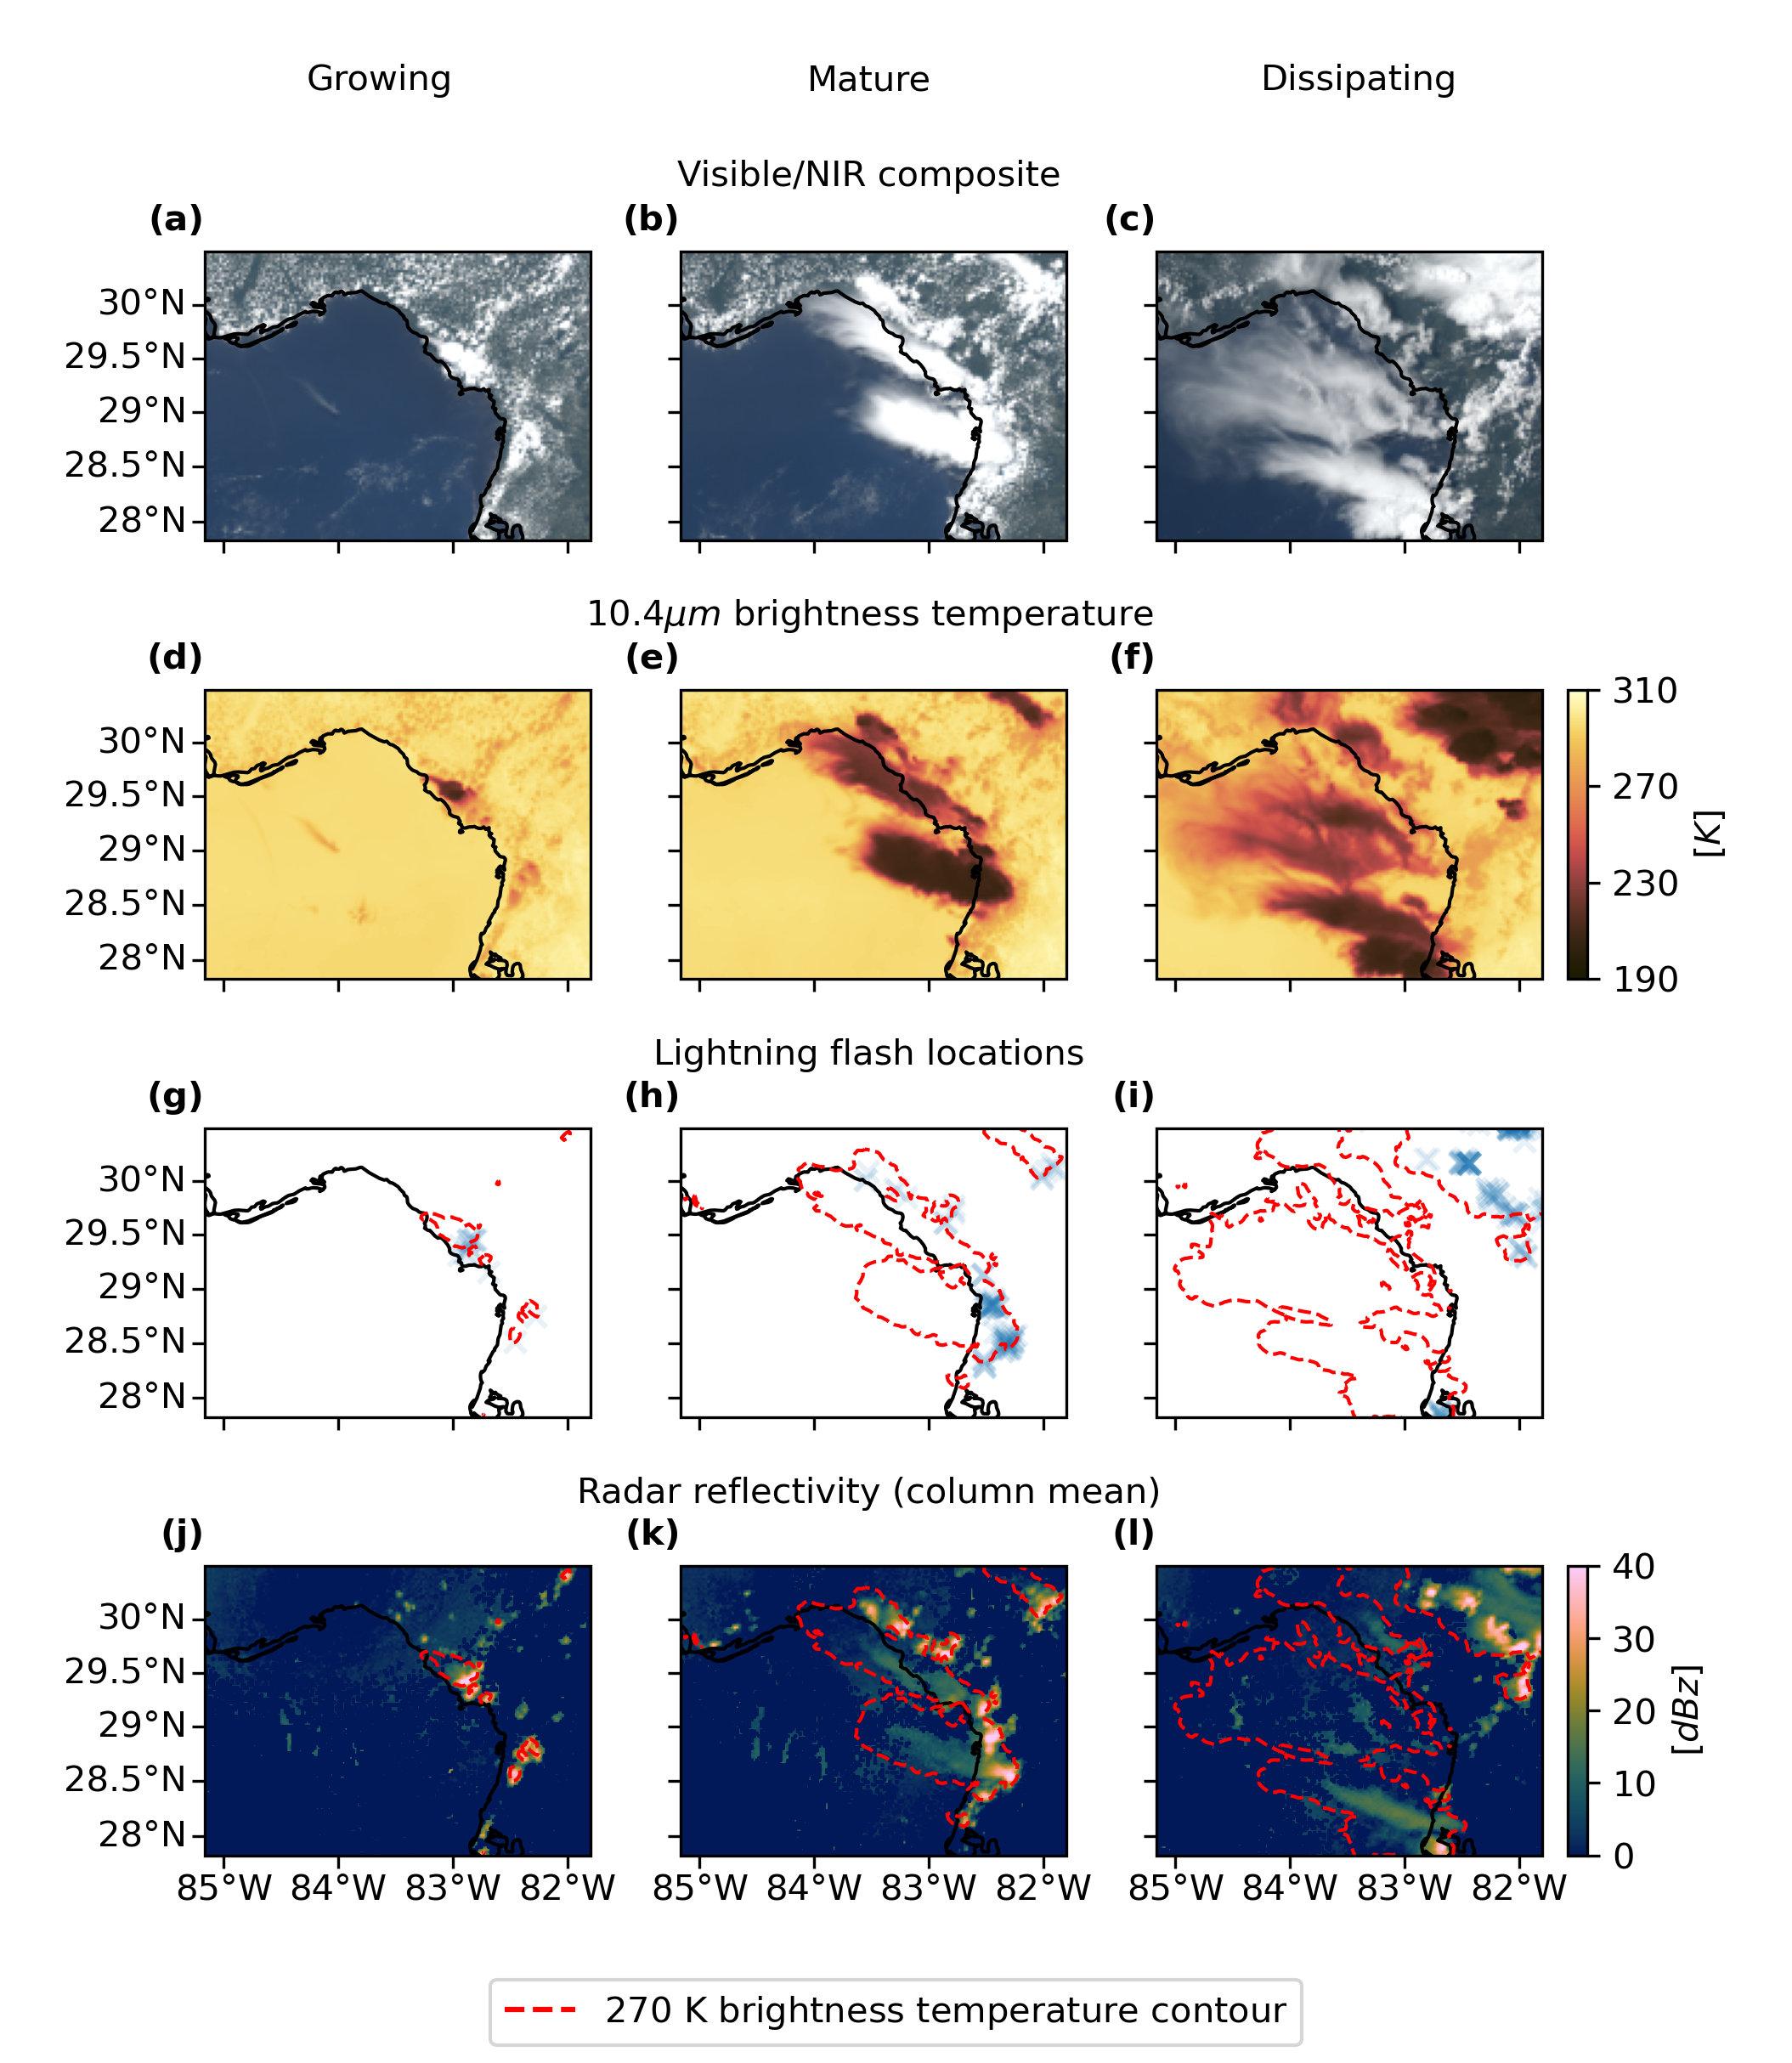
\includegraphics[width=\textwidth]{figures/chapter1_01.png}
    \caption[
    Observations of a cluster of \acrshort{dcc}s over North-West Florida throughout three stages of their lifecycle
    ]{
    Observations of a cluster of \acrshort{dcc}s over North-West Florida throughout three stages of their lifecycle. This cluster of \acrshort{dcc}s occurred on the afternoon of 19\textsuperscript{th} June 2018. The `growing' column was observed at 17:00 \acrshort{utc}, the `mature' column at 19:00 \acrshort{utc}, and the `dissipating' column at 21:00 \acrshort{utc}. The four rows show observations of \acrshort{abi} visible/\acrshort{nir} composites (a,b,c), and 10.4\,\unit{\mu m} \acrshort{bt} (d,e,f); lightning flash locations observed by \acrshort{glm} (g,h,i), and column mean radar reflectivity observed by \acrshort{nexrad} (j,k,l). Note that, unless otherwise specified, this case study is used for all subsequent figures in this chapter.
    }
    \label{fig:compare_sat_radar_glm}
\end{figure}


These instruments are capable of observing the extent of the anvil clouds associated with \acrshort{dcc}s over their entire lifecycle, even after convective activity has ceased (fig.~\ref{fig:compare_sat_radar_glm}\,f).
This is of particular importance due to the influence of anvil cloud radiative forcing on the climate, their response to temperature change \citep{bony_thermodynamic_2016, hartmann_tropical_2016, ceppi_cloud_2017, gasparini_what_2019} and possible feedbacks on subsequent convective activity.
The newest generation of geostationary imaging satellites offers greater opportunities for the study of \acrshort{dcc}s due to their high spatial and temporal resolution -- allowing the detection and tracking of individual convective cores \citep{heikenfeld_tobac_2019} -- and also due to their high signal-to-noise ratio allowing research quality observations \citep{iacovazzi_goes-16_2020}.

The detection and tracking of \acrshort{dcc}s from satellite imagery remains challenging due to the inability to directly observe the convection that drives \acrshort{dcc}s using passive visible and \acrshort{ir} observations.
This is unlike radar and lightning observations, which can directly observe deep convection due to the strong correlations between core updraft intensity and radar reflectivity and polarisation \citep{austin_relation_1987,  zipser_vertical_1994},  and lightning flash occurrence \citep{williams_relationship_1989}.
Instead, a proxy for convective activity must be used to detect deep convection in visible/\acrshort{ir} satellite imagery.
The approaches used for this can generally be separated into two separate methods. 
Firstly, the use of thresholds on \acrshort{bt} or other observed fields, which are capable of detecting \acrshort{dcc} anvil clouds \citep[e.g.][]{schmetz_monitoring_1997, hong_detection_2005, schroder_deep_2009}.
Secondly, the detection of rapidly growing cloud tops by observing changes in the anvil cloud-top radiative cooling, or by other similar approximations of cloud growth \citep{zinner_cb-tram_2008, bedka_objective_2010}.

Developing a detection method using either approach is made challenging by the dynamic nature of \acrshort{dcc}s themselves.
\acrshort{dcc} cores typically have diameters of around 10\,\unit{km}, and updraft velocities on the order of 10\,\unit{m s\textsuperscript{-1}} \citep{weisman_mesoscale_2015}, and exist for 1-3 hours \citep{chen_diurnal_1997}.
Large, mesoscale convective systems (consisting of multiple cores joined by a single large anvil \citep{roca_simple_2017}) may span areas several orders of magnitude larger than isolated \acrshort{dcc}s \citep{houze_mesoscale_2004}, and typically exist to 10-20 hours or longer \citep{chen_diurnal_1997}.
The life cycle of a \acrshort{dcc} can be split into three phases: an initiation or growing phase, a mature phase and a dissipating phase after the cessation of convective activity \citep{wall_life_2018}.
There exists a significant difference between the diurnal cycles of deep convection over the land and over the ocean, with observed \acrshort{dcc}s over land clustered towards the end of the day \citep{taylor_evaluating_2017}.


%f
\begin{figure}[tp]
    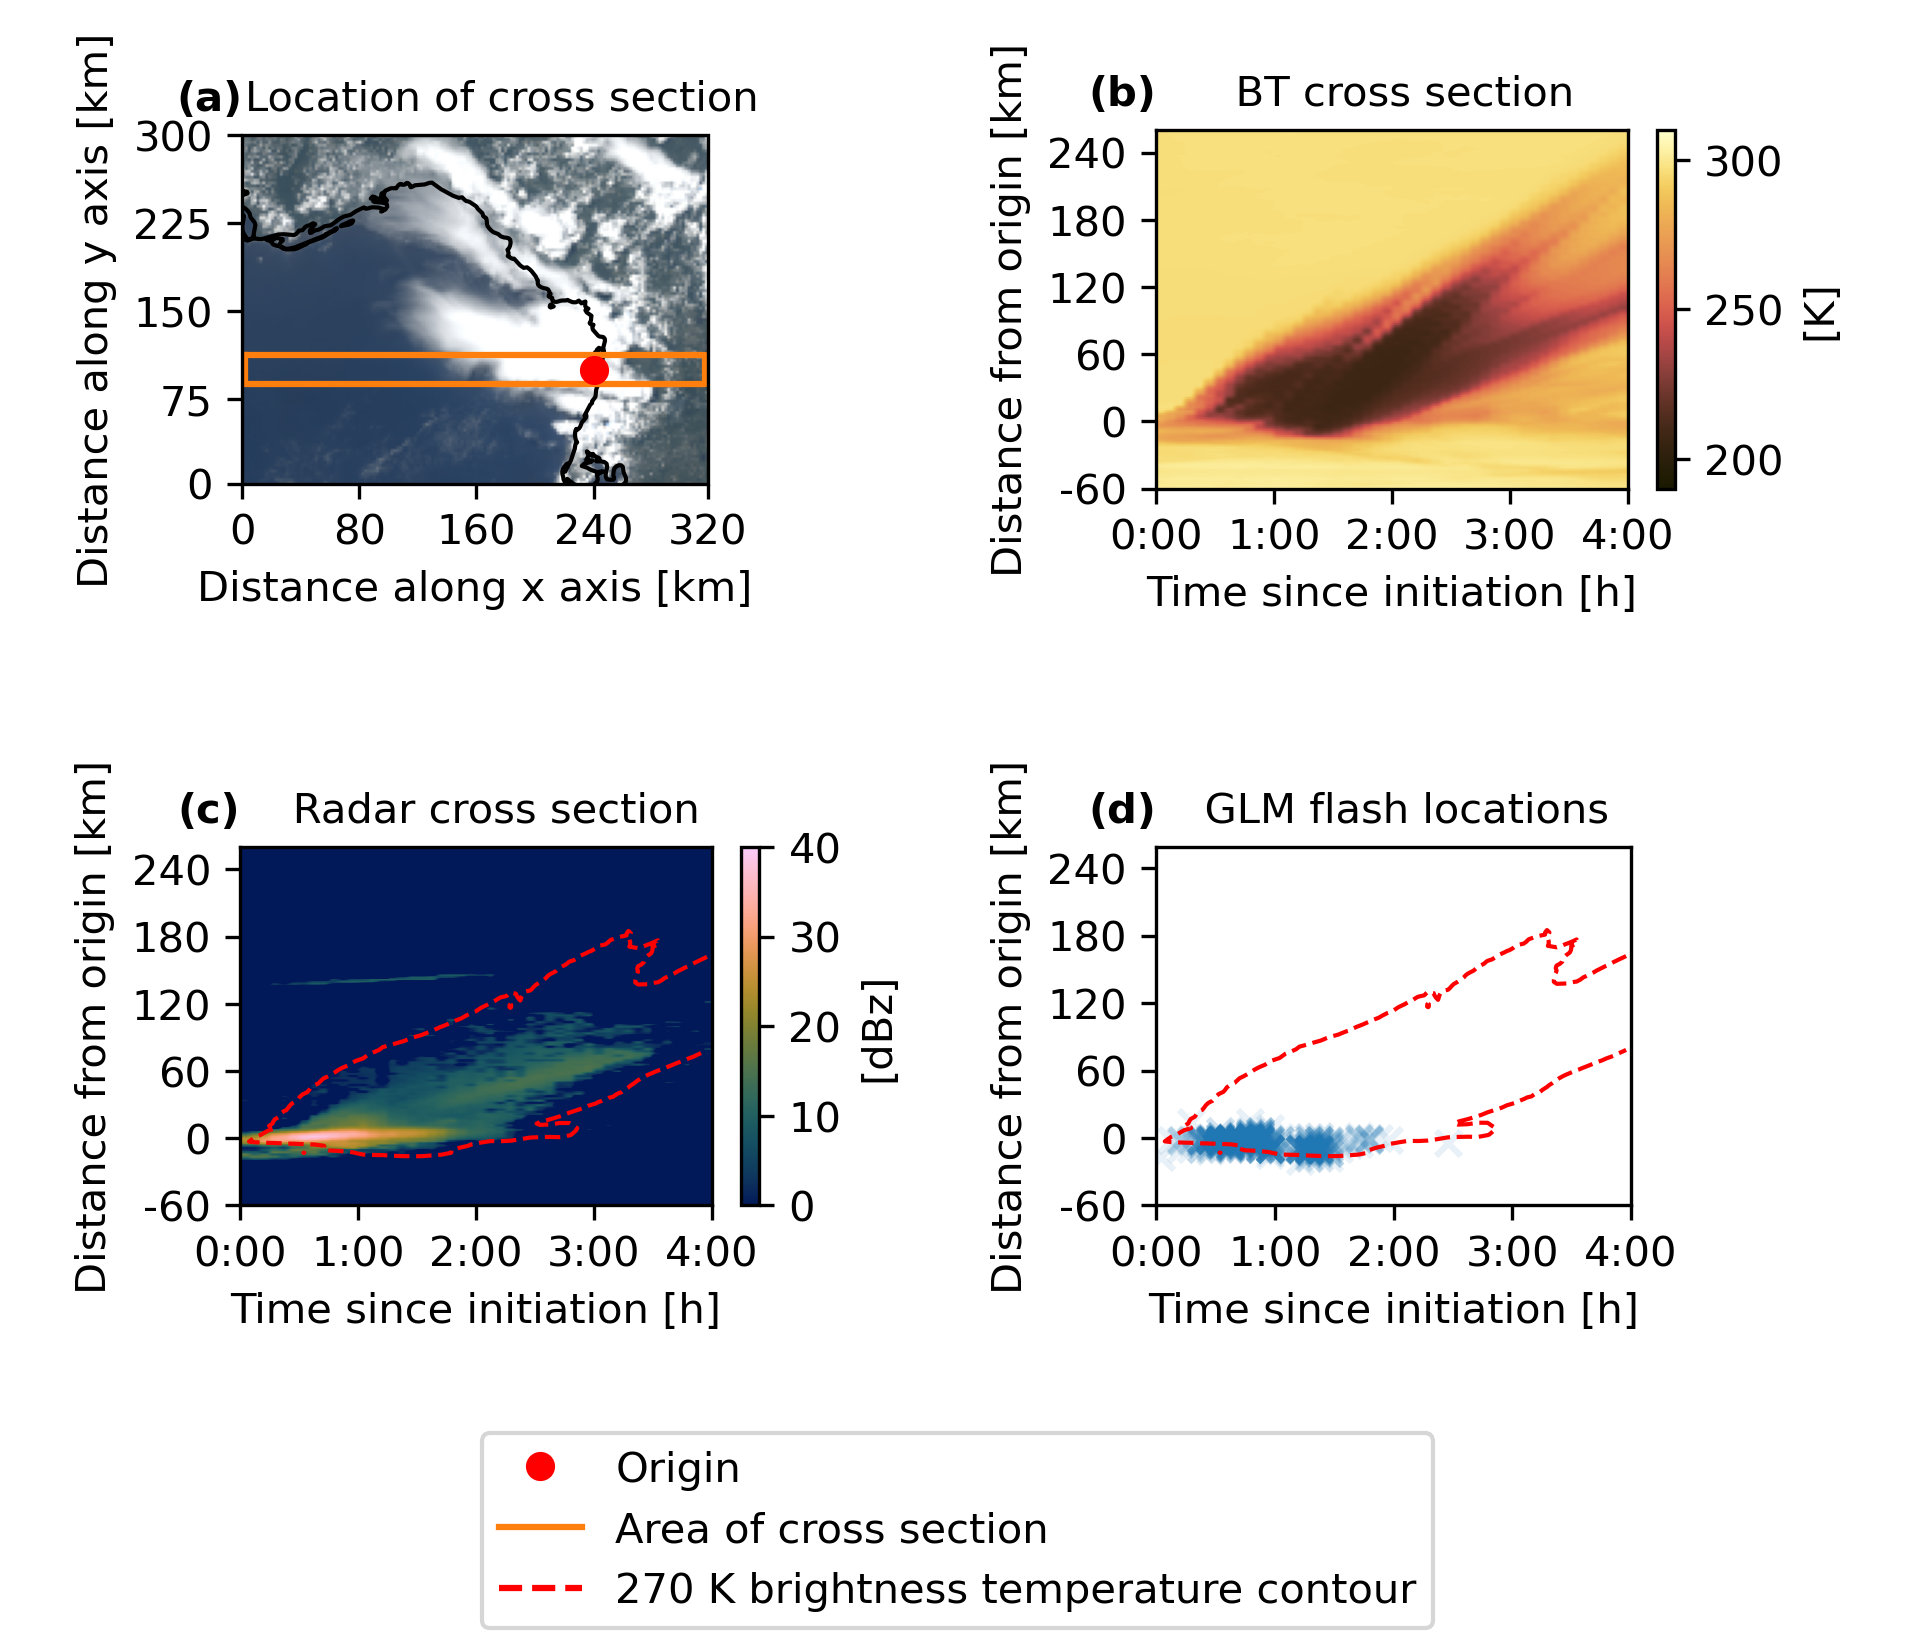
\includegraphics[width=\textwidth]{figures/chapter1_02.png}
    \caption[
    Cross sections of the \acrshort{dcc} observed in figure~\ref{fig:compare_sat_radar_glm} as they develop over time
    ]{
    Cross sections of the \acrshort{dcc} observed in figure~\ref{fig:compare_sat_radar_glm} as they develop over time. a.: The location of the cross-section within the observed \acrshort{dcc}. The mean of values is taken in the North-South axis. b.: \acrshort{abi} 10.8\,\unit{\mu m} \acrshort{bt}, showing rapid cooling for the first 30 minutes, followed by an expanding region of anvil cloud that begins to thin and warm after 2-3 hours. c.: Column mean radar reflectivity, showing the presence and location of the convective core. d.: Lightning flash locations observed by \acrshort{glm}, which closely match the core observed by \acrshort{nexrad}. Initiation occurred at 82.0\,\textdegree W 28.5\,\textdegree N at a time of 17:00 \acrshort{utc}.
    }
    \label{fig:dcc_over_time}
\end{figure}


The difficulties of detecting \acrshort{dcc}s using various proxy approaches are demonstrated by the cross-sections of an observed \acrshort{dcc} over time in fig.~\ref{fig:dcc_over_time}.
The observed \acrshort{bt} of the \acrshort{dcc} anvil cloud shows wide variation over time, with the anvil cloud thinning due to dissipation after the end of convective activity which results in a warmer \acrshort{bt} due to greater signal from the surface.
This variety of observed temperatures leads to large differences in the chosen threshold value between different algorithms \citep[see discussion in][]{bennartz_convective_2012}.
This choice of the threshold value is further complicated due to the overlap in observed \acrshort{bt}s between \acrshort{dcc} anvils and non-convective clouds \citep{konduru_new_2013}.
As a result, any detection method using a \acrshort{bt} threshold must compromise between missed detection of \acrshort{dcc}s, or false detections of non-\acrshort{dcc} clouds.

The cooling of the cloud top is only visible for a short period during the initial phase of the \acrshort{dcc}, before the anvil cloud top reaches the tropopause temperature after approximately 30 minutes.
As a result, any method that solely relies on detecting the growth of the \acrshort{dcc} will be unable to detect the anvil cloud after this initial growth phase has ended.
While such algorithms provide accurate detection of these early phases of \acrshort{dcc} growth \citep{zinner_validation_2013}, they are unable to continue tracking the anvil cloud after convective activity is no longer observed.

\citet{fiolleau_algorithm_2013} identified this need to compromise on the accuracy of detecting \acrshort{dcc}s as a problem caused by the commonly used two-step framework for detecting and tracking \acrshort{dcc}s.
In this framework, \acrshort{dcc}s are first detected in individual images, and then linked together over time in sequences of images.
As a result, the detection method chosen must be capable of detecting \acrshort{dcc}s at each individual time step in order to track their entire lifecycle.
Instead \citet{fiolleau_algorithm_2013} implemented a single-step framework for mesoscale convective systems that treats a sequence of images as a `3-D' volume (consisting of two spatial dimensions and one temporal dimension), and performs detection and tracking simultaneously by applying a watershed method over both spatial and temporal dimensions.
Whereas this approach was successful for large, mesoscale systems, where the advection of the anvil is small compared to the overall anvil area, it is less capable of tracking small, rapidly moving convective cores.
To improve the tracking of small \acrshort{dcc}s, we have developed a semi-Lagrangian framework for single-step detection and tracking which accounts for the motion of \acrshort{dcc}s using optical flow.

By utilising the semi-Lagrangian framework, we can combine the best elements of both growth-based and threshold-based detection methods.
We show that it is possible to detect growing \acrshort{dcc}s to a high degree of accuracy using methods similar to those of \citet{zinner_cb-tram_2008}, and then extend the detected \acrshort{dcc} over the entire anvil cloud using the 3-D watershed method of \citet{fiolleau_algorithm_2013}.
This framework reduces the compromise required between the rate of missed \acrshort{dcc}s and falsely detected \acrshort{dcc}s, improving the overall accuracy of our detection method compared to existing approaches.
Furthermore, this method allows the anvil cloud to be detected and tracked even after the region of cloud top cooling is no longer detected.
Finally, the 3-D method handles the merging and splitting of intersecting \acrshort{dcc}s by detecting all \acrshort{dcc}s that intersect at any point during their lifetime as a merged object.


\section{Data}

Three sources of data are used throughout this chapter.
Primarily, visible and \acrshort{ir} imagery from \acrshort{abi} aboard the \acrshort{goes}-16 weather satellite is used for the detection of \acrshort{dcc}s.
Secondarily, observations from the \acrshort{nexrad} weather radar network and the \acrshort{glm} (also aboard \acrshort{goes}-16) are used to assess and validate the tracking and detection method presented here.


\subsection{Advanced Baseline Imager} \label{sec:abi_data}


The \acrshort{abi} is a visible and \acrshort{ir} radiometer aboard the \acrshort{goes}-16 series of weather satellites \citep{schmit_closer_2016}.
\acrshort{goes}-16, also known as \acrshort{goes}-East, is situated in a geostationary orbit at 75.2\,\textdegree W above the equator, providing a field of view (or `Earth-disc') covering most of the western hemisphere, including all of South America and most of North America.
\acrshort{abi} has 16 channels operating in a range of spectral bands in the visible, \acrshort{nir} and thermal-\acrshort{ir}.
The majority of these channels have a resolution of 2\,\unit{km} at the sub-satellite point, although this reduces to approximately 3\,\unit{km} across most of the \acrfull{conus} due to the satellite viewing angle.
\acrshort{abi} operates in a flexible scan mode, making observations of the \acrshort{conus} once every 5 minutes, the full disc every 10 minutes (15 minutes prior to April 2019), and two mesoscale regions of approximately 2500 by 2500\,\unit{km} every minute.
Additionally, it is capable of scanning the full disc every five minutes if no other scans are performed.
This combination of high spatial and temporal resolution makes \acrshort{abi} suitable for detecting and tracking small and developing \acrshort{dcc}s, as well as providing the spatial coverage to also track large mesoscale convective systems \citep{heikenfeld_tobac_2019}.


%t
\begin{table}[tb]
\centering
\begin{tabular}{lrrr}
\tophline
Instrument                                              & \acrshort{abi}   & \acrshort{seviri}    & Imager \\
\middlehline
Temporal resolution (\unit{minutes})                    & 5     & 15        & 30 \\
Nadir spatial resolution (\unit{k m})                   & 2     & 3         & 4 (8 for \acrshort{wv}) \\
Number of \acrshort{ir} \acrshort{lw} window channels                         & 3     & 2         & 2 \\
Number of \acrshort{ir} \acrshort{wv} channels                                & 3     & 2         & 1 \\
% Noise equivalent temperature  (\unit{K} @ 300\,\unit{K})  & 0.1   & 0.25      & 0.09 \\
\bottomhline
\end{tabular}
\caption[
Comparison of data from \acrshort{abi} to that from older geostationary instruments
]{
Comparison of data from \acrshort{abi} to that from older geostationary instruments\; \acrshort{seviri} aboard the second generation meteosat satellites, and the imager aboard the second generation \acrshort{goes}.
} % Table Footnotes
\label{table:abi_comparison}
\end{table}

Compared to older geostationary instruments, \acrshort{abi} has higher spatial and temporal resolution, and more channels in both the \acrshort{lw} \acrshort{ir} window spectrum and the \acrshort{lw} \acrshort{ir} \acrfull{wv} spectrum (table \ref{table:abi_comparison}) \citep{iacovazzi_goes-16_2020}.
This, combined with many of the channels being derived from those aboard the Visible Infrared Imaging Radiometer Suite, make the data from \acrshort{abi} more suitable for research purposes than that from older instruments \citep{heidinger_chapter_2020}.
Several artifacts are known to occur in \acrshort{abi} imagery \citep{gunshor_goes-r_2020}.
Although the majority of these artifacts are removed using the data quality flag associated with the \acrshort{abi} data, we have found a number of cases in which bad detector stripes (described in section 3.2 of \citealp{gunshor_goes-r_2020}) are not flagged in the data. 
These regions are detected separately, and replaced with missing data prior to cloud tracking.

In this chapter, we have used the \acrshort{abi} level 2 \acrfull{mcmip} which provides calibrated reflectances and \acrshort{bt}s for all \acrshort{abi} channels on a common grid \citep{schmit_chapter_2020}, using the 5-minute frequency imagery provided over the \acrshort{conus} region.
The case study shown in the figures throughout this chapter is for a subset of the \acrshort{conus} scan region centred at 83.7\,\textdegree W, 29.2\,\textdegree N, over the time period of 17:00:00 to 21:00:00 \acrshort{utc} on the 19th June 2018.
Validation was performed on the \acrshort{conus} scan region over the entirety of 2018.
All data has been sourced through the \acrshort{noaa} Big Data Program.



\subsubsection{Selection of \acrshort{abi} Channels and Channel Combinations} \label{sec:abi_channels}

In order to have an equal performance during both day and nighttime, a selection of \acrshort{lw} \acrshort{ir} \acrshort{abi} channels are used for the detection and tracking of \acrshort{dcc}s (see fig.~\ref{fig:abi_channels}). 
These channels consist of the 10.4\,\unit{\mu m} and 12.4\,\unit{\mu m} \acrshort{lw} (also known as the clean and dirty window channels respectively due to the presence of \acrshort{wv} in the latter), and the upper and lower troposphere \acrshort{wv} channels at 6.2\,\unit{\mu m} and 7.3\,\unit{\mu m} respectively.
Whereas the \acrshort{lw} window \acrshort{ir} \acrshort{bt} is commonly used for the detection of anvil clouds using threshold-based methods, we have decided not to use it for this purpose in this method due to the wide range of \acrshort{bt}s observed within anvil clouds, and the variance of anvil cloud temperature because of changes in tropopause temperature due to meteorology and latitude.
However, the information contained within this field is used for the optical flow calculation of the cloud motion field.


%f
\begin{figure}[tp]
    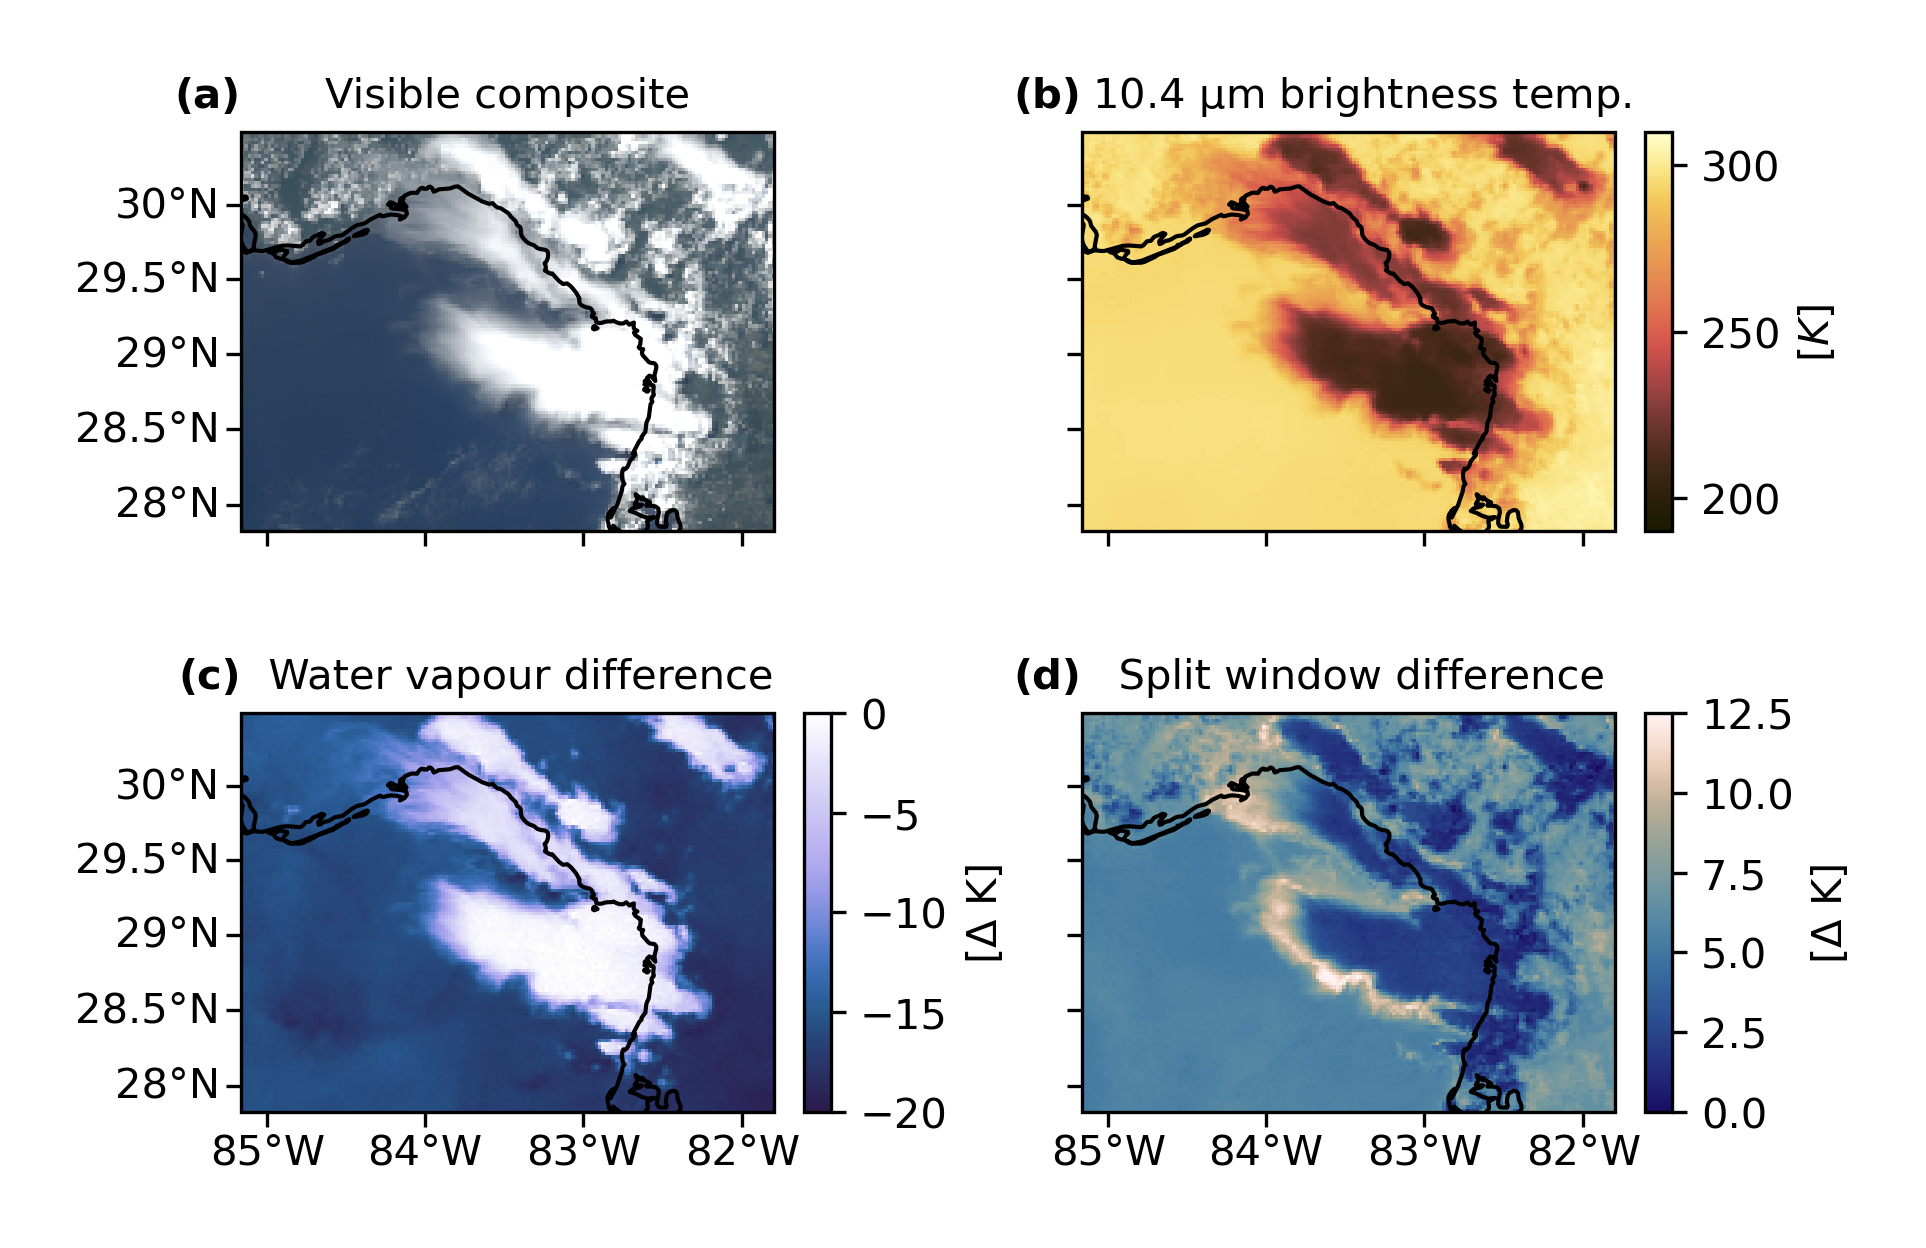
\includegraphics[width=\textwidth]{figures/chapter1_03.png}
    \caption[
    \acrshort{abi} channels and channel differences used with the detection and tracking algorithm
    ]{
    \acrshort{abi} channels and channel differences used with the detection and tracking algorithm. a.: A composite of visible and \acrshort{nir} channels. b.: The 10.4\,\unit{\mu m} \acrshort{bt}, or clean \acrshort{lw} window channel, which can differentiate clouds at all altitudes by their \acrshort{bt}. c.: the \acrshort{wvd} combination, of the 6.2\,\unit{\mu m} upper troposphere \acrshort{wv} channel minus the 7.3\,\unit{\mu m} lower troposphere \acrshort{wv} channel, which is strongly negative for clear sky and low cloud, but approaches positive values for thick, high clouds. d.: the \acrshort{swd} combination of the 10.4\,\unit{\mu m} clean \acrshort{lw} window channel minus the 12.4\,\unit{\mu m} dirty \acrshort{lw} window channel, which is near zero for thick clouds, around\,\unit{K} for clear skies and approximately 10\,\unit{K} for thin, ice clouds.
    }
    \label{fig:abi_channels}
\end{figure}


Two additional combinations of channels are used to detect areas of \acrshort{dcc} anvil. 
The \acrfull{wvd} combination (fig.~\ref{fig:abi_channels}\,c) of the upper troposphere \acrshort{wv} channel minus the lower troposphere \acrshort{wv} channel has been shown to provide a high detection rate for \acrshort{dcc}s \citep{muller_role_2018, muller_novel_2019}.
In clear sky or low cloud conditions, \acrshort{wvd} shows the temperature difference between the upper and lower troposphere of generally around -20\,\unit{K}. 
While the 6.2\,\unit{\mu m} has an additional contribution from stratospheric \acrshort{wv} \citep{schmetz_monitoring_1997}, this does not have a significant effect on the \acrshort{wvd} due to the small size of this absorption (fig.~\ref{fig:abi_vertical_weighting}.
Because both the \acrshort{wv} channels are strongly absorbed by \acrshort{wv} in the lower troposphere, the \acrshort{wvd} field is not affected by surface and low altitude features and so provides a clear distinction between thick, high clouds and the background across a wide range of situations.
\citet{muller_novel_2019} found that a threshold of -5\,\unit{K} gave a high detection rate of anvil clouds.
Furthermore, as the \acrshort{wvd} values are relative to the lower stratosphere temperatures, this field is much less affected by location and meteorology than the \acrshort{lw} \acrshort{ir} channels.
However, the \acrshort{wvd} is still prone to the false detections of non-convective clouds when using a thresholding method as it cannot directly distinguish between thick, high-altitude clouds that are associated with deep convection and those that are not.

\begin{figure}[tp]
    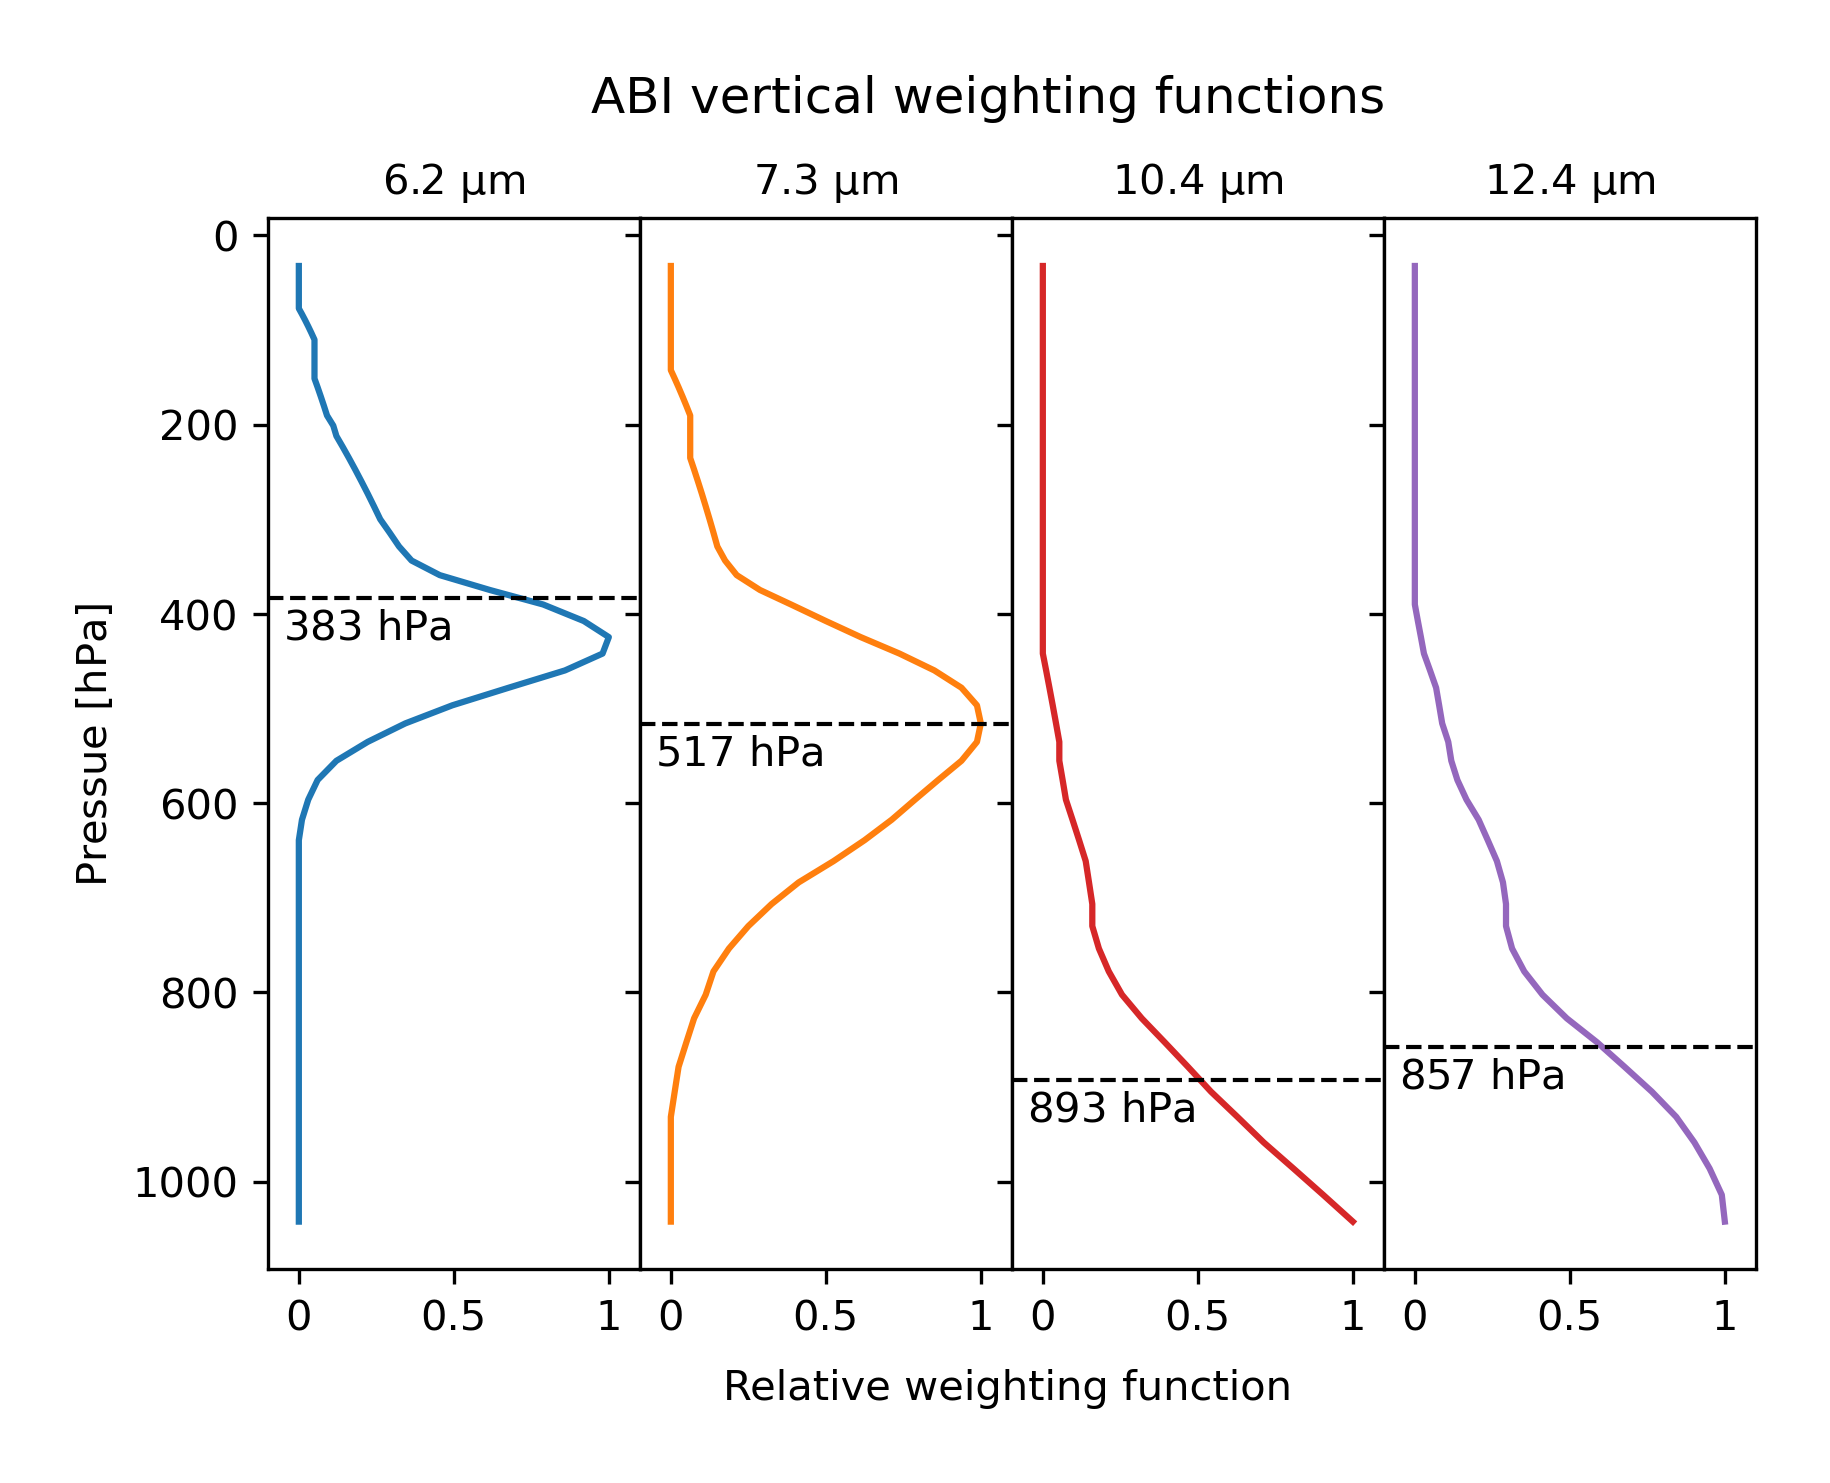
\includegraphics[width=0.9\textwidth]{figures/chapter1_04.png}
    \caption[
    Clear sky vertical weighting functions for the 6.2, 7.3, 10.4 and 12.4\,\unit{\mu m} \acrshort{abi} channels
    ]{
    Clear sky vertical weighting functions for the 6.2, 7.3, 10.4 and 12.4\,\unit{\mu m} \acrshort{abi} channels calculated from rawinsonde profiles measured on 12:00:00 \acrshort{utc} 2020/08/10 at the Tampa RAOB station (KTBW - 72210). The dashed lines and associated pressure values show the weighted average emission height for each channel. Data from {https://cimss.ssec.wisc.edu/goes-wf/plot-viewer/\#/plot-viewer/plot/raob/abi16/default/20200810\_1200Z/72210}
    }
    \label{fig:abi_vertical_weighting}
\end{figure}

The \acrfull{swd}, consisting of the clean \acrshort{ir} window channel minus the dirty \acrshort{ir} window channel (fig.~\ref{fig:abi_channels}\,d), aids in the detection and separation of optically thin anvil cloud (including cirrus outflow) from optically thick anvil due to the difference in ice particle emissivity between these two channels \citep{heidinger_gazing_2009}.
As a result, this combination displays warm temperatures of around 10\,\unit{K} for thin, ice clouds, near 0\,\unit{K} for thick clouds, and approximately 5\,\unit{K} for clear skies due to the contribution of boundary layer \acrshort{wv}.
The \acrshort{swd} is, however, also sensitive to low-level clouds and low-level \acrshort{wv} concentrations, and so cannot be used alone to detect \acrshort{dcc}s.
It remains important to consider the \acrshort{swd} field due to the difficulty in separating anvil clouds from cirrus when using \acrshort{lw} \acrshort{ir} \acrshort{bt} alone \citep{hong_detection_2005}. 
By subtracting the value of the \acrshort{swd} from the \acrshort{wvd}, we can reduce the sensitivity of our detection scheme to thin cirrus clouds, reducing the rate of erroneous detections.
Additionally, adding the \acrshort{swd} field to the \acrshort{wvd} field can enhance the appearance of cirrus, enabling the detection of thin ice clouds associated with cirrus outflow and dissipating anvils.

Figure~\ref{fig:abi_vertical_weighting} shows the clear sky vertical weighing functions for the 6.2, 7.3, 10.4 and 12.4\,\unit{\mu m} \acrshort{abi} channels.
The weighting functions are calculated using a radiative transfer model with temperature and humidity profiles observed by rawinsonde observations on 12:00:00 \acrshort{utc} 2020/08/10 at the Tampa RAOB station (KTBW - 72210). 


%t
\begin{table}[tb]
\centering
\begin{tabular}{lrrr}
\tophline
Instrument   & wavelength   & \acrshort{nedt} [300\,K]    & \acrshort{nedt} [220\,K] \\
\middlehline
ABI (GOES--16)         & 6.2\,\unit{\mu m} & 0.013\,K & 0.117\,K\\
             & 7.4\,\unit{\mu m} & 0.024\,K & 0.137\,K\\
             & 10.4\,\unit{\mu m} & 0.028\,K & 0.082\,K\\
             & 12.4\,\unit{\mu m} & 0.023\,K & 0.052\,K\\
\middlehline
SEVIRI (MSG--11)       & 6.2\,\unit{\mu m} & 0.05\,K & 0.45\,K\\
             & 7.3\,\unit{\mu m} & 0.05\,K & 0.29\,K\\
             & 10.8\,\unit{\mu m} & 0.06\,K & 0.17\,K\\
             & 12.0\,\unit{\mu m} & 0.10\,K & 0.24\,K\\
\bottomhline
\end{tabular}
\caption[
Operational \acrshort{nedt} for the \acrshort{abi} and \acrshort{seviri} instruments. 
]{
Operational \acrshort{nedt} for the \acrshort{abi} and \acrshort{seviri} instruments. \acrshort{nedt} is shown both at 300\,K and at 220\,K. \acrshort{abi} data is from {https://www.star.nesdis.noaa.gov/GOESCal/G16\_ABI\_INST\_CAL\_daily\_allmode.php}; \acrshort{seviri} data is from \citet{pili_inorbit_2016}.
} % Table Footnotes
\label{table:channel_nedt}
\end{table}

Measured, on-orbit instrument noise for the \acrshort{abi} and \acrshort{seviri} instruments are provided for each of the four channels selected for use in table~\ref{table:channel_nedt}.
The \acrfull{nedt} values are provided at a reference temperature of 300\,K.
However, as \acrshort{nedt} varies with temperature, it is also important to consider the noise at the colder temperatures typical of anvil clouds.
\acrshort{nedt} at 220\,K were calculated by multiplying the \acrshort{nedt} at 300\,K by the ratio of the partial derivative of the Planck function at 300\,K to that at 220\,K.
This results in a noticeably larger \acrshort{nedt} at the lower temperature, in particular for the \acrshort{wv} channels due to the difference in the gradient of the Planck function between the two temperatures.
Propagating these uncertainties provides estimates of the noise in the \acrshort{wvd} and \acrshort{swd} combinations of 0.180\,K and 0.097\,K respectively for \acrshort{abi}, and 0.54\,K and 0.29\,K for \acrshort{seviri}.

In addition to the \acrshort{nedt}, there are several sources of systematic errors which may affect the observed \acrshort{bt} and channel differences.
Any bias in the \acrshort{abi} and \acrshort{seviri} channels are accounted for in calibration.
Limb darkening at larger satellite zenith angles is harder to account for.
This will have two impacts on the channel differences.
Firstly, it will increase the height at which \acrshort{wv} emissions are observed in the 6.2 and 7.4\,\unit{\mu m} channels, increasing the height at which clouds can be observed.
Secondly, for the \acrshort{swd} combination it may reduce the difference between the two channels, as a higher zenith angles the path length through a cloud layer is longer for the same thickness of cloud, and therefore the difference in temperature will be less between the two channels.

In addition, environmental conditions may affect both the \acrshort{wvd} and \acrshort{swd} combinations.
Changes in humidity may affect the height at which the \acrshort{wvd} is sensitive to clouds, with lower humidity resulting in sensitivity at lower cloud heights.
In addition, the difference between the surface temperature and the cloud temperature will affect the \acrshort{swd}, as the temperature difference is due to a combination of cloud emission and surface emission with a ratio that varies across the two channels.
As a result, if the difference between the cloud and surface temperatures is smaller, so too will be the \acrshort{swd}.
While these biases cannot be removed from the data without retrieving the cloud properties, the choice of methods for cloud detection can limit their impact on the results of detection and tracking.


\subsection{Geostationary Lightning Mapper}

The \acrshort{glm} is also mounted on \acrshort{goes}-16 and detects lightning flashes using an optical transient detector.
The optical transient detector utilises a single, narrow-band \acrshort{nir} channel centred on 777\,\unit{nm} \citep{orville_absolute_1984} to detect momentary changes in brightness associated with lightning events at a frequency of 400\,\unit{\mu s} \citep{christian_global_2003}, providing a 70\,\% minimum efficiency of detection \citep{goodman_goes-r_2013}.
\acrshort{glm} has the same field of view as the \acrshort{abi} instrument, albeit with a lower spatial resolution of 8\,\unit{km} at the sub-satellite point.

As lightning observations are strongly correlated with \acrshort{dcc}s, data from \acrshort{glm} is used to validate the detection of \acrshort{dcc}s using \acrshort{abi}.
The level 2 \acrshort{glm} lightning cluster-filter algorithm product provides a dataset of events, groups and flashes processed from the \acrshort{glm} data \citep{peterson_research_2019}, and filters artifacts from the level 1 \acrshort{glm} data \citep{peterson_removing_2020}.
From this dataset, we extract detected flashes as evidence of \acrshort{dcc} occurrence.
These locations are then processed by mapping their frequency onto the \acrshort{abi} grid for validation of the algorithm.

\subsection{Next Generation Radar}

\acrshort{nexrad}, also known by its technical name \acrfull{wsr88d}, is a network of weather radars operated by the National Weather Service across the USA \citep{crum_wsr-88d_1993}.
\acrshort{wsr88d} operates in the S-band spectrum, between 2700 and 3000\,\unit{MHz}.
\acrshort{nexrad} stations scan at a range of elevations, typically between 0.5\textdegree\ and 19.5\textdegree\ above horizontal, with a typical scan cycle taking between 4\,\sfrac{1}{2} and 6~minutes, comparable to the temporal sampling of \acrshort{abi} over the \acrshort{conus} region.

Cloud radar reflectivity is proportional to the droplet number density and the droplet radius to the sixth power, making it particularly sensitive to convective rainfall \citep{yau_short_1989}.
As a result, cloud radar observations are ideal for showing the locations of convective cores \citep{austin_relation_1987, rosenfeld_general_1993, zipser_vertical_1994}, and in this chapter it is used to qualitatively assess our ability to detect developing convective cores using \acrshort{abi}.
Level 2 \acrshort{nexrad} radar reflectivity observations from multiple sites are gridded to the same resolution as \acrshort{abi}, and column mean reflectivity is calculated between the altitudes of 2.5 and 15\,\unit{k m}.

\section{Theory} \label{sec:detection_theory}

To better understand how \acrshort{dcc}s appear in \acrshort{goes} \acrshort{abi} observations, a series of experiments were performed using a radiative transfer model.
These experiments were performed using libRadTran v2.0.4 \citep{emde_libradtran_2016}, utilising the DISORT radiative transfer solver \citep{buras_new_2011} and the REPTRAN absorbtion parameterisation \citep{gasteiger_representative_2014}.
The experiments were run using the pyLRT wrapper for libRadTran \citep{gryspeerdt_pylrt_2024}.
A tropical atmospheric profile was used to represent the atmospheric conditions under which deep convection typically occurs.
A complete list of the options used to set up the radiative transfer model across all simulations is provided in table \ref{table:libradtran}.

\begin{table}[tb]
\centering
\begin{tabular}{lll}
\tophline
Option          & Value                 & Description                   \\ 
\middlehline
rte\_solver     & disort                & DISORT solver                 \\
source          & thermal               & thermal \acrshort{ir} spectra \\
wavelength      & 3000--15000           & 3--15\,\unit{\mu m}           \\
output\_user    & lambda edir eup uu    & wavelength, direct, diffuse   \\
                &                       &irradiance and all radiances   \\
zout            & 0 TOA                 & surface and \acrshort{toa}    \\
albedo          & 0.5                   & surface albedo                \\
umu             & -1.0, 1.0             & downward \& upward            \\
sza             & 0                     & solar zenith angle            \\
mol\_abs\_param & reptran fine          & REPTRAN parameterisation      \\
atmosphere\_file& afglt.dat             & tropical atmosphere profile   \\
liquid microphysics& Hu                 & \citet{hu_accurate_1993} parameterisation \\
ice microphysics& Fu                    & \citet{fu_accurate_1996} parameterisation \\
\bottomhline
\end{tabular}
\caption[
    Selected options for the libRadTran simulations
    ]{
    Selected options for the libRadTran simulations. All other parameters are left as defaults.
    }
\label{table:libradtran}
\end{table}

In each of the simulations, a cloud layer is included in addition to these options to represent a \acrshort{dcc} in different phases of the lifecycle.
For liquid cloud droplets we use the Hu parameterisation \citep{hu_accurate_1993}, and for ice particles we use the Fu scheme \citep{fu_accurate_1996, fu_accurate_1998}. To show how the simulated clouds are observed by \acrshort{goes}-16, we calculate \acrshort{bt} from the simulated radiances, and then integrate over the spectral response function of each of the \acrshort{abi} channels.

\subsection{Observing growing convective cores}\label{sec:theory_core}

The first experiment aims to represent how a vertically developing \acrshort{dcc} core would appear in \acrshort{abi} observations.
To do so, we run a series of simulations with increasing cloud top heights between 1 and 15\,\unit{k m} at 1\,\unit{k m} intervals.
These cloud layers are given a base height of 0\,\unit{k m}, \acrfull{lwc} of 1,000\,\unit{g m^{-2}}, and droplet \acrfull{re} of 15\,\unit{\mu m}.
These values were chosen to represent typical conditions seen in a convective core.
Although we use liquid droplets at all altitudes, simulations with ice cloud droplets showed negligible differences for cloud layers of this thickness.

Figure~\ref{fig:cloud_height_spectra} shows \acrshort{bt} spectra for increasing cloud height, with the spectral response functions of the ten thermal \acrshort{ir} \acrshort{abi} channels plotted in the background.
With such a large \acrshort{lwc}, the \acrshort{bt} matches the \acrshort{ctt} apart from the absorption regions of CO\textsubscript{2} (4.2--4.5\,\unit{\mu m} and \>13.2\,\unit{\mu m}) and ozone (9.4--10.2\,\unit{\mu m}), and the \acrshort{wv} absorption for low-level clouds (5--8\,\unit{\mu m}).


\begin{figure}[tp]
    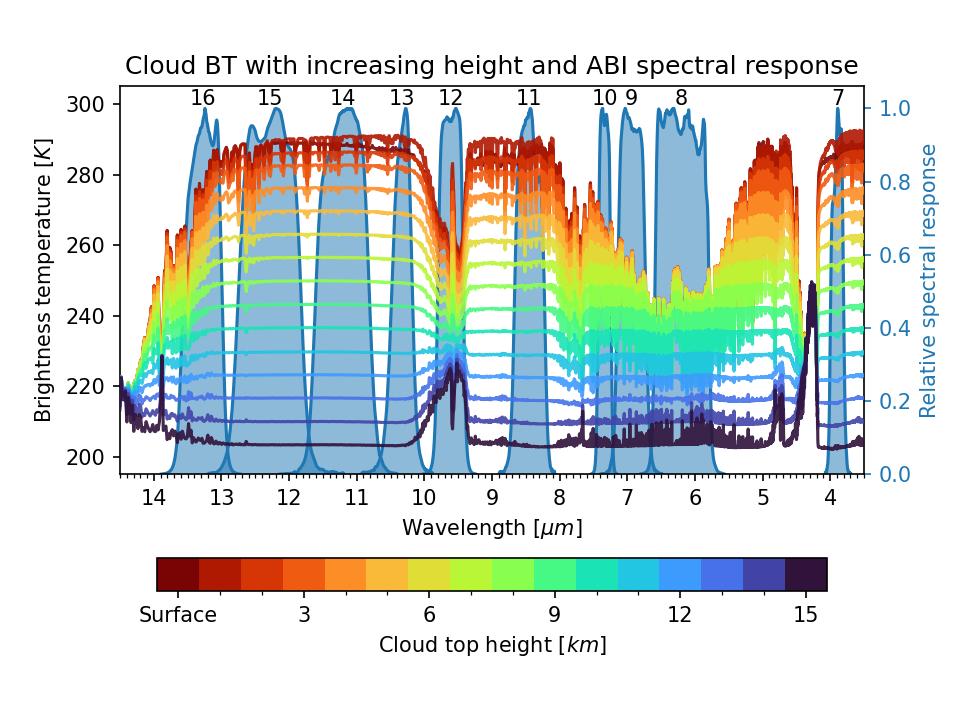
\includegraphics[width=\textwidth]{figures/chapter1_05.png}
    \caption[
    \acrshort{toa} \acrshort{bt} spectra for a simulated cloud representing a \acrshort{dcc} core at heights between 1 and 15\,\unit{k m}
    ]{
    \acrshort{toa} \acrshort{bt} spectra for a simulated cloud representing a \acrshort{dcc} core at heights between 1 and 15\,\unit{k m}, indicating that the largest difference in \acrshort{bt} are seen in the \acrshort{lw} window regions. The filled blue areas in the background show the relative spectral response functions for each of the \acrshort{lw} \acrshort{abi} channels.
    }
    \label{fig:cloud_height_spectra}
\end{figure}


The change in observed \acrshort{bt} with height for the 6.2, 7.3, 10.4, and 12.4\,\unit{\mu m} \acrshort{bt} channels along with the \acrshort{wvd} and \acrshort{swd} is plotted in Fig.~\ref{fig:cloud_height_channels}. 
Above 3\,\unit{k m }, the 10.4 and 12.4\,\unit{\mu m} channels show a constant decrease observed \acrshort{bt} at the moist pseudo-adiabatic lapse rate of 6\,\unit{K}.
Due to the contribution of \acrshort{wv} to the 6.2 and 7.3\,\unit{\mu m} channels at lower \acrfull{cth}, the \acrshort{wvd} shows the most response to vertical development between 6 and 10\,\unit{k m}.
The \acrshort{swd} shows a response to clouds developing at a low altitude.
It has been proposed that this can be used to detect the onset of convection in clear sky conditions before other observations, such as cloud radars \citep{lindsey_use_2014, lindsey_using_2018}.


\begin{figure}[tp]
    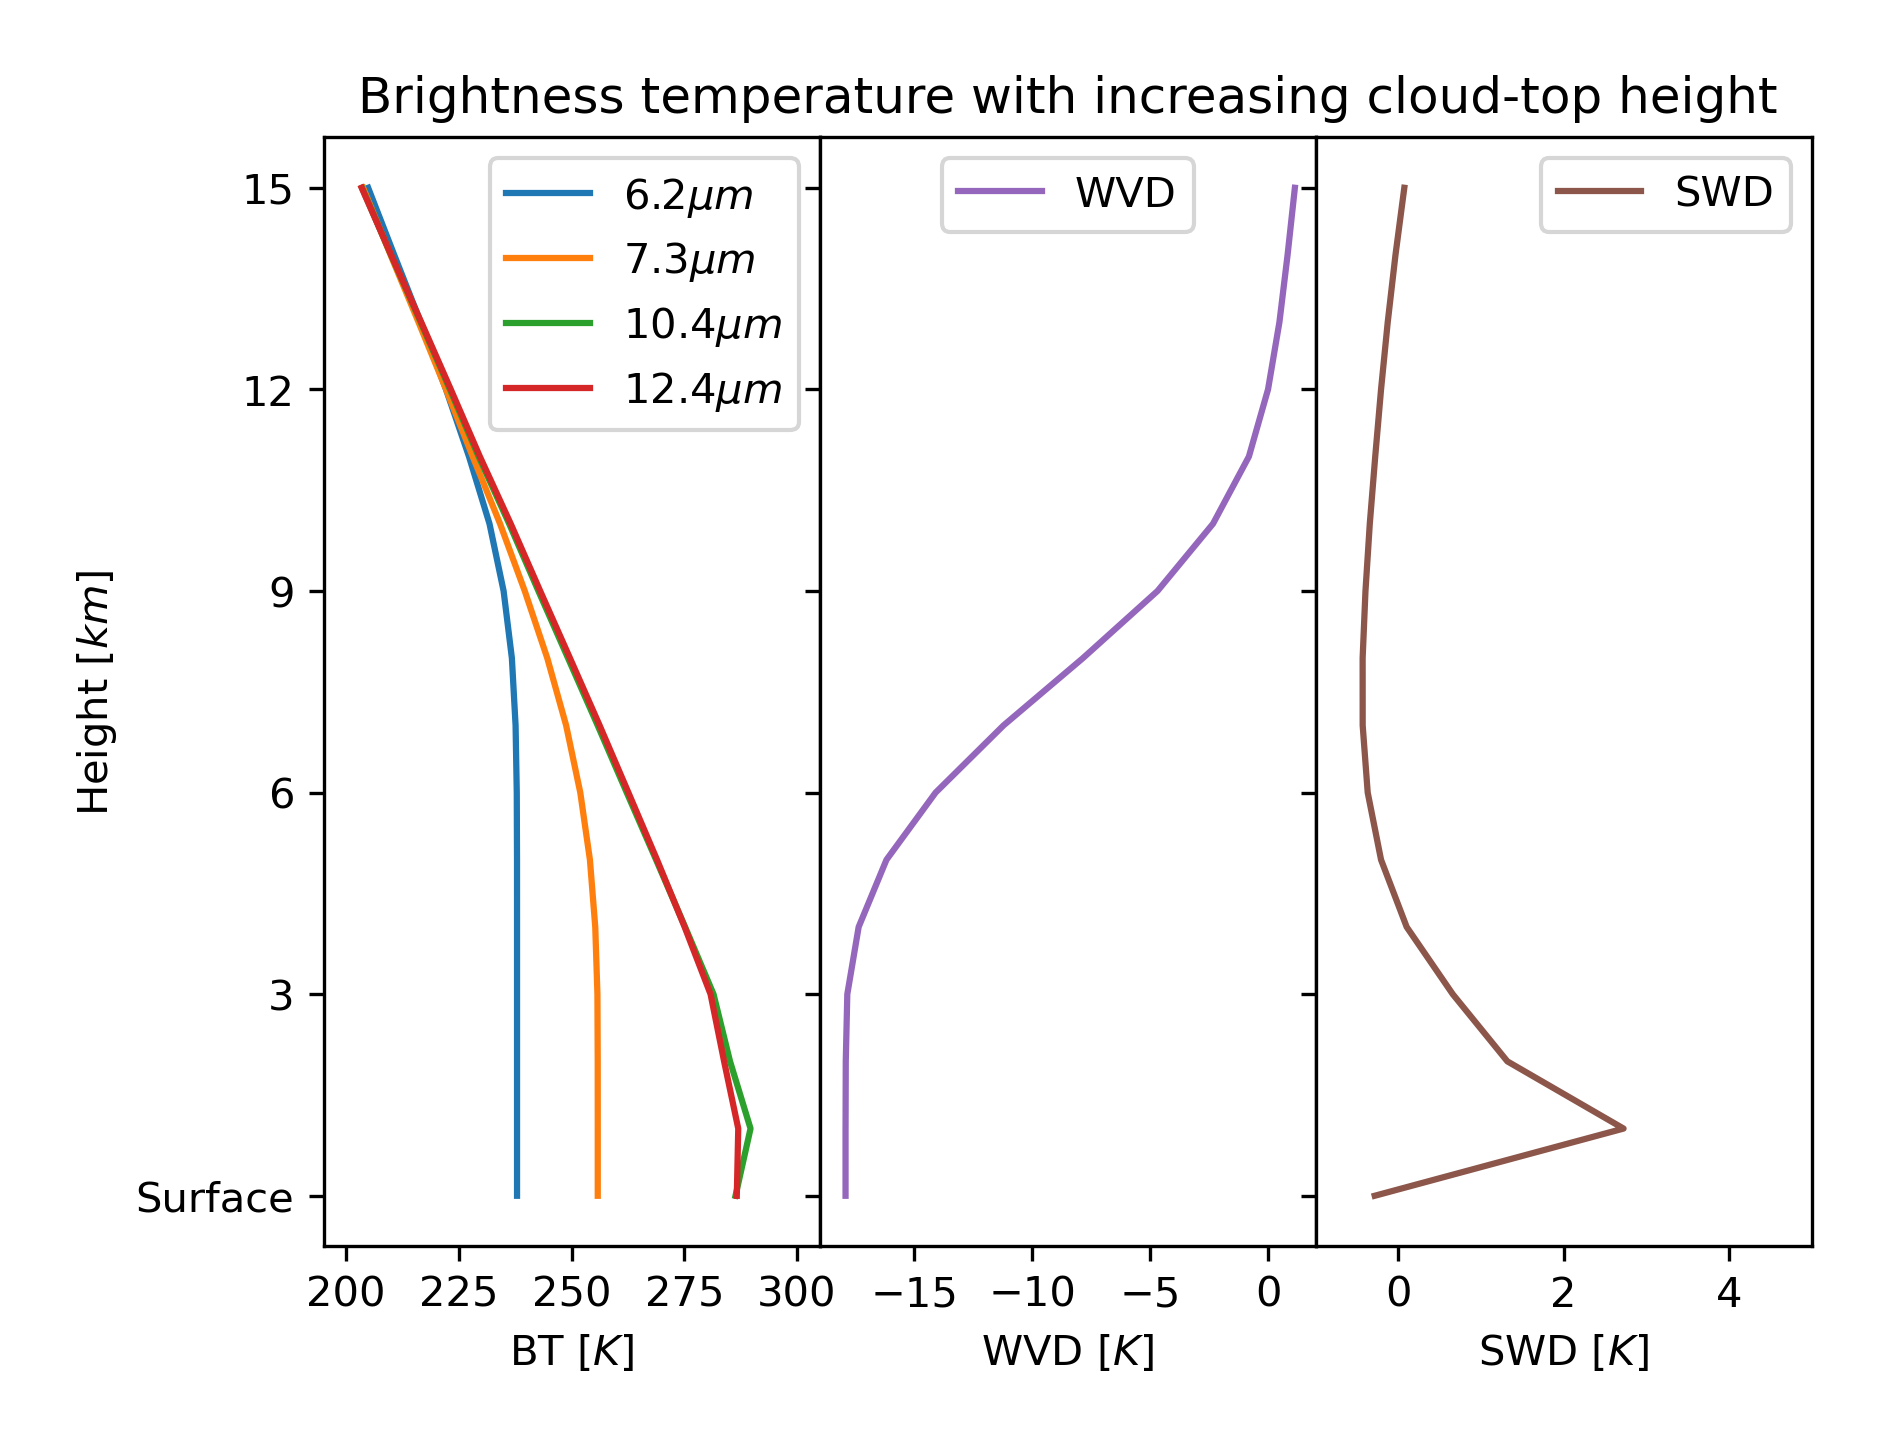
\includegraphics[width=0.9\textwidth]{figures/chapter1_06.png}
    \caption[
    Simulated observations of the 6.2, 7.3, 10.4 and 12.4\,\unit{\mu m} \acrshort{abi} channels, \acrshort{wvd} and \acrshort{swd} for a \acrshort{dcc} core of increasing height
    ]{
    Simulated observations of the 6.2, 7.3, 10.4 and 12.4\,\unit{\mu m} \acrshort{abi} channels, \acrshort{wvd} and \acrshort{swd} for a \acrshort{dcc} core of increasing height.
    }
    \label{fig:cloud_height_channels}
\end{figure}


Figure~\ref{fig:cloud_height_cooling_rates} shows the change of observed \acrshort{bt} in units of K$\cdot\mathrm{minute^{-1}}$ for a convective core rising at a rate of 1\,\unit{ms^{-1}}.
Above 3\,km, the 10.4\,\unit{\mu m} shows a consistent cooling of 0.5\,K$\cdot\mathrm{minute^{-1}}$.
\citet{roberts_nowcasting_2003} found a threshold for severe convection of 8\,\unit{K} cooling over 15~minutes, or approximately 0.5\,K$\cdot\mathrm{minute^{-1}}$, which would represent a cloud top vertical velocity of 1.25\,\unit{m s^{-1}} according to our simulation.
The \acrshort{wvd} shows a maximum rate of change between 7 and 8\,\unit{km}, with a warming rate of half the magnitude of the \acrshort{bt} cooling rate.


\begin{figure}[tp]
    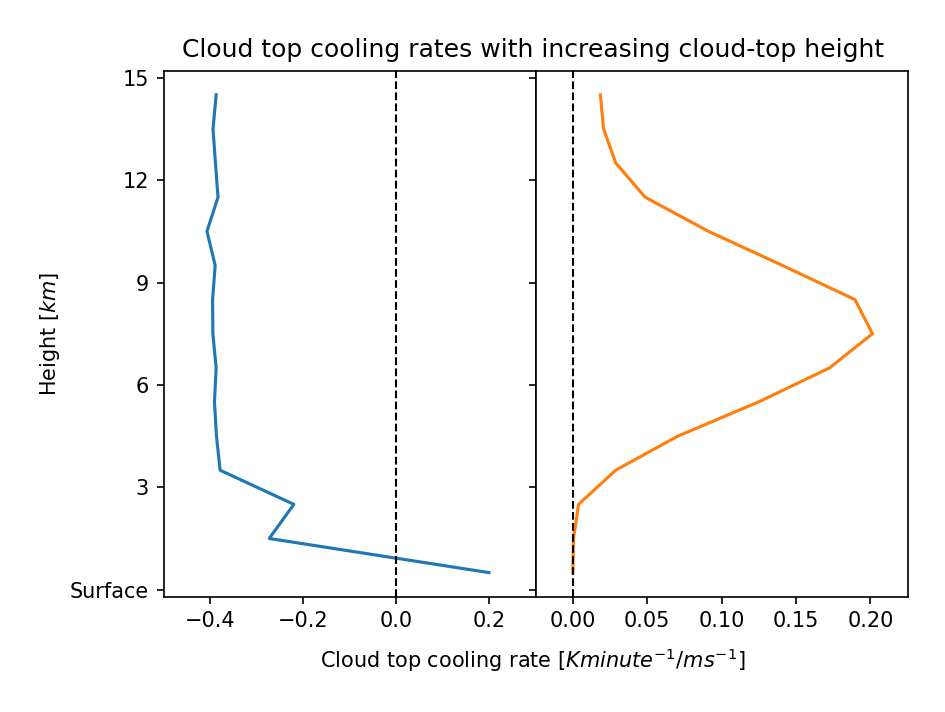
\includegraphics[width=0.9\textwidth]{figures/chapter1_07.png}
    \caption[
    Simulated observed cooling rates of the 10.4\,\unit{\mu m} \acrshort{abi} channels and the \acrshort{wvd} combination for a convective core growing at a rate of 1\,\unit{m s^{-1}}
    ]{
    Simulated observed cooling rates of the 10.4\,\unit{\mu m} \acrshort{abi} channels and the \acrshort{wvd} combination for a convective core growing at a rate of 1\,\unit{m s^{-1}}.
    }
    \label{fig:cloud_height_cooling_rates}
\end{figure}

Using the \acrshort{nedt} values provided in table~\ref{table:channel_nedt}, the uncertainty due to sensor noise in the \acrshort{bt} difference over a five--minute period is approximately 0.047\,K$\cdot \mathrm{minute^{-1}}$, or just less than 10\% of the threshold given by \citet{roberts_nowcasting_2003}.
By averaging the cooling rates over 5 pixels and a 15--minute time period the uncertainty is reduced to 0.012\,K$\cdot \mathrm{minute^{-1}}$, or less than 2.5\%.

Overall, we see from this experiment that the 10.4\,\unit{\mu m} \acrshort{bt} channel from \acrshort{abi} can be used to clearly identify a vertically developing core across a wide range of altitudes.
On the other hand, the \acrshort{wvd} is only sensitive to vertically developing clouds in a narrower range of altitudes, and shows a weaker rate of \acrshort{bt} change.
However, this sensitivity to vertical development at a mid to high altitude may help distinguish between \acrshort{dcc}s and other, vertically developed clouds at lower altitudes, such as cumulus congestus.

It should be noted that these simulations were performed with the cloud temperature in equilibrium with the surrounding environment, this is not the case for a convective core which will be warmer than the surrounding air.
Taking 6\,\unit{K/km} as a typical value for the moist pseudo--adiabatic lapse rate, the cooling rate for a convective cloud top rising at 1\,\unit{ms^{-1}} is 0.36\,$\mathrm{K \cdot minute^{-1}}$.
This is similar to the value shown in fig.~\ref{fig:cloud_height_cooling_rates} for the 10.4\,\unit{\mu m} \acrshort{bt}.
In addition, due to mixing of surrounding air with the convective cloud top, we expect that the observed temperature profile of the core will be somewhere between that of the environment profile and the moist pseudo--adiabatic lapse rate.
In general the temperature of the top of convective cores varies very little from the surrounding environment \citep{zipser_cumulonimbus_1980}.
Furthermore, overshooting tops should continue to cool with the moist pseudo--adiabatic lapse rate, indicating that the \acrshort{bt} difference is also capable of detecting overshooting convective cores.

\subsection{Observing anvil clouds} \label{sec:theory_anvil}

In the second experiment, we investigate how anvil clouds of different \acrfull{od} appear in \acrshort{abi} observations.
The simulations were run with an ice cloud with \acrshort{cth} at 14\,\unit{k m}, cloud base height at 12\,\unit{km} and cloud top \acrshort{re} of 20\,\unit{\mu m}, aiming to represent the typical properties of a dissipating anvil cloud \citep{sokol_tropical_2020}.
This simulation was then run for a range of \acrshort{od} between 0.125 and 10, with intervals of 0.125 between 0.125 and 1, 0.25 between 1 and 2, 0.5 between 2 and 5, and 1 between 5 and 10.

\begin{figure}[tp]
    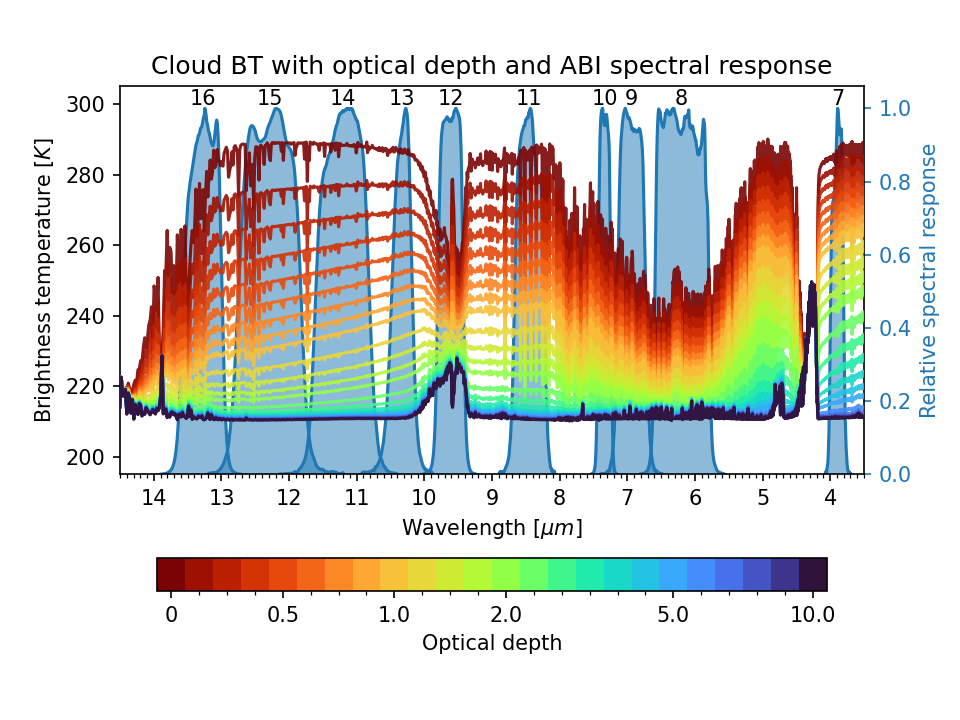
\includegraphics[width=\textwidth]{figures/chapter1_08.png}
    \caption[
    \acrshort{toa} \acrshort{bt} spectra for a simulated anvil cloud with optical thickness between 0 and 10
    ]{
    \acrshort{toa} \acrshort{bt} spectra for a simulated anvil cloud with optical thickness between 0 and 10. 
    }
    \label{fig:optical_depth_spectra}
\end{figure}

\acrshort{bt} spectra for these simulations are shown in Fig.~\ref{fig:optical_depth_spectra}, along with the \acrshort{abi} spectral response functions as in Fig.~\ref{fig:cloud_height_spectra}.
As before, we see absorption due to CO\textsubscript{2}, ozone, and \acrshort{wv}.
Unlike the simulations in section \ref{sec:theory_core} however, we see a difference in the \acrshort{bt} spectra across the \acrshort{lw} window (10--13\,\unit{\mu m}) for clouds with \acrshort{od} between 0 and 2, with colder \acrshort{bt} at longer wavelengths.
This is due to the difference in ice emissivity across this range of wavelengths \citep{fu_radiation_2015}.
As the emissivity of ice particles reduces for wavelengths at 10\,\unit{\mu m} and below there is a greater contribution from the atmosphere below the cloud layer and, as a result, warmer \acrshort{bt}s are observed.
It should be noted that this difference is dependent on the size of the ice particles, with smaller \acrshort{re} resulting in a larger difference in emissivity \citep{dubuisson_sensitivity_2008}.


\begin{figure}[tp]
    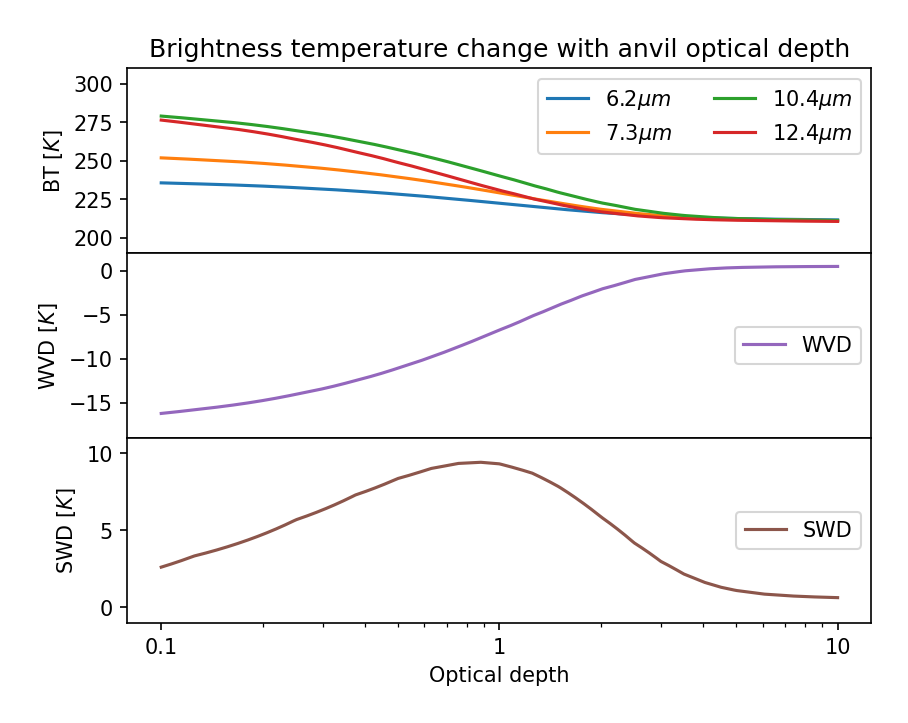
\includegraphics[width=0.9\textwidth]{figures/chapter1_09.png}
    \caption[
    Simulated \acrshort{abi} \acrshort{bt} observations for a \acrshort{dcc} anvil of decreasing optical depth
    ]{
    Simulated \acrshort{abi} \acrshort{bt} observations for a \acrshort{dcc} anvil of decreasing optical depth for the 6.2, 7.3, 10.4, and 12.4\,\unit{\mu m} \acrshort{bt} channels, the \acrshort{wvd} and the \acrshort{swd}.
    }
    \label{fig:optical_depth_channels}
\end{figure}

Figure~\ref{fig:optical_depth_channels} shows simulated \acrshort{abi} observations for the 6.2, 7.3, 10.4, and 12.4\,\unit{\mu m} \acrshort{bt} channels, the \acrshort{wvd} and the \acrshort{swd} for a range of \acrshort{od} between 0.1 and 10.
At high \acrshort{od}, all channels show a cold \acrshort{bt} close to that of the \acrshort{ctt}, however, for \acrshort{od} below 3, the increased contribution from the atmosphere below results in warmer \acrshort{bt}.
The \acrshort{wvd} similarly shows a more negative \acrshort{bt} difference at \acrshort{od} below 3, with a continual decrease for smaller \acrshort{od}.
The \acrshort{swd} however shows an increasingly positive \acrshort{bt} difference for \acrshort{od} below 5, peaking at 10\,\unit{K} around 1~\acrshort{od}.
Below this \acrshort{od} the \acrshort{swd} decreases towards smaller positive values.
As a result, the \acrshort{swd} has the potential to detect thin anvil cirrus at much lower \acrshort{od} than \acrshort{bt} channels or \acrshort{wvd}, down to values around 0.25~\acrfull{od}.

While the \acrshort{bt}, \acrshort{wvd} and \acrshort{swd} are plotted in fig.~\ref{fig:optical_depth_channels} as a function of \acrshort{od} only, other factors may influence the observations.
Changes in cloud height will affect the observed \acrshort{bt}, as higher anvils will have lower temperatures and vice versa.
The \acrshort{wvd} should be unaffected by cloud height as long as the cloud is above heights at which \acrshort{wv} contributes to the vertical weighting functions (fig.~\ref{fig:abi_vertical_weighting}), and above 12\,km there is little change with height (fig.~\ref{fig:cloud_height_cooling_rates}). 
Changes in tropospheric humidity will affect the \acrshort{wvd} as this will change the height of the weighting function response and hence the height at which the \acrshort{wvd} is sensitive to clouds.
As the majority of \acrshort{dcc}s are expected to occur in relatively humid environments we expect that this effect will be minimal.
However, in particularly cold, dry conditions this may result in lower level clouds being erroneously detected as anvils.
Finally, the \acrshort{swd} has some sensitivity to \acrshort{re}, as larger particles show a smaller difference in emissivity between 10 and 12\,\unit{\mu m}.
The effect of this is small, and the peak \acrshort{swd} remains present at the same optical depth.


\section{Method} \label{sec:tracking_method}

We present here a novel method for detecting and tracking both the growing cores and anvils clouds of \acrshort{dcc}s, consisting of the following steps:

\begin{enumerate}
    \item Ingest of \acrshort{lw} \acrshort{ir} \acrshort{bt} fields from geostationary satellite imagery, including calculation of \acrshort{wvd} and \acrshort{swd} fields from \acrshort{ir} \acrshort{wv} and \acrshort{lw} \acrshort{ir} window channels.
    \item Calculation of optical flow vectors to be used as an \textit{a priori} estimate of cloud motion for use in the semi-lagrangian framework.
    \item Detection of growing \acrshort{dcc} cores using cloud top cooling rate.
    \item Detection of thick and thin anvil clouds associated with detected cores using a semi-lagrangian "3D" watershedding method. 
    \item Grouping of cores into multi-core systems, calculation of statistics and validation using lightning observations.
\end{enumerate}



\subsection{Estimation of cloud motion vectors using optical flow} \label{sec:optical_flow}

The retrieval of \acrshort{amv}s has been performed since the earliest geostationary satellite observations \citep{menzel_cloud_2001}.
\acrshort{amv}s provide information about the motion of clouds in the atmosphere, including \acrshort{dcc}s \citep{bedka_application_2005}, and are routinely generated for the majority of operational geostationary earth observation satellites, including \acrshort{goes}-16 \citep{daniels_algorithm_nodate}. 
However, although \acrshort{amv}s may provide useful information about the motion of \acrshort{dcc}s, the non-geostrophic nature of wind fields in these conditions may result in the \acrshort{amv}s being calculated inaccurately or rejected by quality control checks \citep{bedka_application_2005}.

Optical flow algorithms are a family of algorithms used to estimate the apparent motion of objects observed in a series of images \citep{aggarwal_computation_1988}. 
A wide range of optical flow algorithms exist, and these have been successfully applied to many computer vision applications. 
It should be noted that optical flow does not necessarily represent the physical motion of an object, but is instead an estimation of the relative motion between an object and the observer and additionally any change in the apparent object (including growing, shrinking or other warping of the object). 

Optical flow algorithms have been previously shown to be accurate for the prediction of \acrshort{amv}s using geostationary satellite images \citep{wu_deriving_2016}, as long as the observations are sufficiently frequent such that the motion of unique features between images is less than the length scale at which neighbouring features can be resolved \citep{bresky_feasibility_2006}.
\citet{heikenfeld_tobac_2019} found that at imaging frequencies of less than 5~minutes the motion of \acrshort{dcc} cores was less than the spacing between neighbouring cores in the majority of cases, indicating that the frequency of the \acrshort{abi} \acrshort{conus} scan region is suitable for calculating optical flow vectors of \acrshort{dcc}s.
The use of optical flow has several advantages over traditional \acrshort{amv}s for the retrieval of \acrshort{dcc} motion vectors: optical flow can be calculated quickly using only two subsequent images and no \textit{a priori} information, aiding in near real-time applications; and also have no requirement for geostrophic balance. 
Optical flow algorithms are routinely used in the nowcasting of convective precipitation, and can be used to provide accurate predictions of \acrshort{dcc} with an hour of lead time using either radar or satellite observations \citep[e.g.][]{bowler_development_2004, bechini_enhanced_2017, woo_operational_2017}.
Optical flow, and similar motion vector techniques, have also been successfully applied to both the detection of developing deep convection \citep{zinner_cb-tram_2008, zhang_locating_2014} and tracking detected deep convective features \citep{senf_size-resolved_2018} separately.

It should be noted that we are using optical flow to estimate the apparent motion of the cloud field between subsequent images, with the aim of using these vectors to map the locations of \acrshort{dcc}s from one step to the next, instead of calculating actual \acrshort{amv}s corresponding to winds.
This approach avoids a number of challenges with the use of optical flow for calculating \acrshort{amv}s including the estimation of the height of estimated flow vectors and the detection of diverging or converging motion vector fields in situations of growing and dissipating clouds respectively.
In the latter case, we aim to include the divergence and convergence within the optical flow vector field to map both the location and shape of observed clouds between time steps.

\subsubsection{Evaluation of Optical Flow Methods}

As different optical flow algorithms may provide better accuracy in different situations \citep{baker_database_2011}, we compare several algorithms to assess their suitability for tracking the motions of \acrshort{dcc}s.
We consider six different optical flow algorithms implemented in the OpenCV library \citep{opencv_library}, which are listed below:

\begin{itemize}
    \item Farnebäck \citep{farneback_two-frame_2003}
    \item \acrfull{dis} \citep{kroeger_fast_2016}
    \item DeepFlow \citep{weinzaepfel_deepflow_2013}
    \item \acrfull{dualtvl1} \citep{zach_duality_2007, perez_tv-l1_2013}
    \item Sparse to Dense \citep{bouguet_pyramidal_1999}
    \item \acrfull{pca}-Flow \citep{wulff_efficient_2015}
\end{itemize}

The first four of these algorithms are dense optical flow methods, which calculate motion vectors for every pixel in the image.
The final two calculate sparse optical flow---motion vectors between detected objects in each image, rather than individual pixels---and then map these to all pixels based on a region segmentation approach.
The sparse to dense and \acrshort{pca}-flow algorithms use the Lucas-Kanade method \citep{lucas_iterative_1981} and the \acrshort{pca} method respectively to calculate the sparse motion vectors.

Each algorithm was applied to a sequence of images from the 10.4\,\unit{\mu m} channel, with the algorithms estimating motion vectors between each consecutive pair of images.
As the methods require 8-bit images, a linear normalisation was applied to the \acrshort{bt} images between each pair's minimum and maximum values.
To improve the accuracy of the detected motion vectors, a variational refinement process \citep{brox_high_2004} is applied to the calculated flow vectors.
This process minimises the energy functional of the pixel value, pixel gradient, and local smoothness to reduce the angular error of the detected flow vectors.
Finally, vectors are calculated both forwards and backward in time between each pair of images, and these two sets of vectors are interpolated to each other's locations and averaged to ensure that they are equal and opposite.

Figure~\ref{fig:opt_flow_comparison} shows the \acrshort{abi} \acrshort{bt} at 19:00:00~\acrshort{utc} (fig.~\ref{fig:opt_flow_comparison}\,a), along with the optical flow vectors calculated by each of the algorithms with the subsequent time step.
For each set of optical flow vectors, the average vector over each 5\texttimes 5-pixel area is plotted by the red arrows, and the vector velocity magnitude is plotted in the background.
The two sparse methods (fig.~\ref{fig:opt_flow_comparison}\,f,g) show a closer match of the areas where optical flow vectors to the edge of the anvil cloud than the dense methods (fig.~\ref{fig:opt_flow_comparison}\,b--e), which have a tendency to smooth the detected vectors over a large area.
Of all the methods, the Farnebäck algorithm tends to produce larger magnitudes, but correctly detects zero flow in areas without clouds, unlike most of the other algorithms.


\begin{figure}[tp]
    \centering
    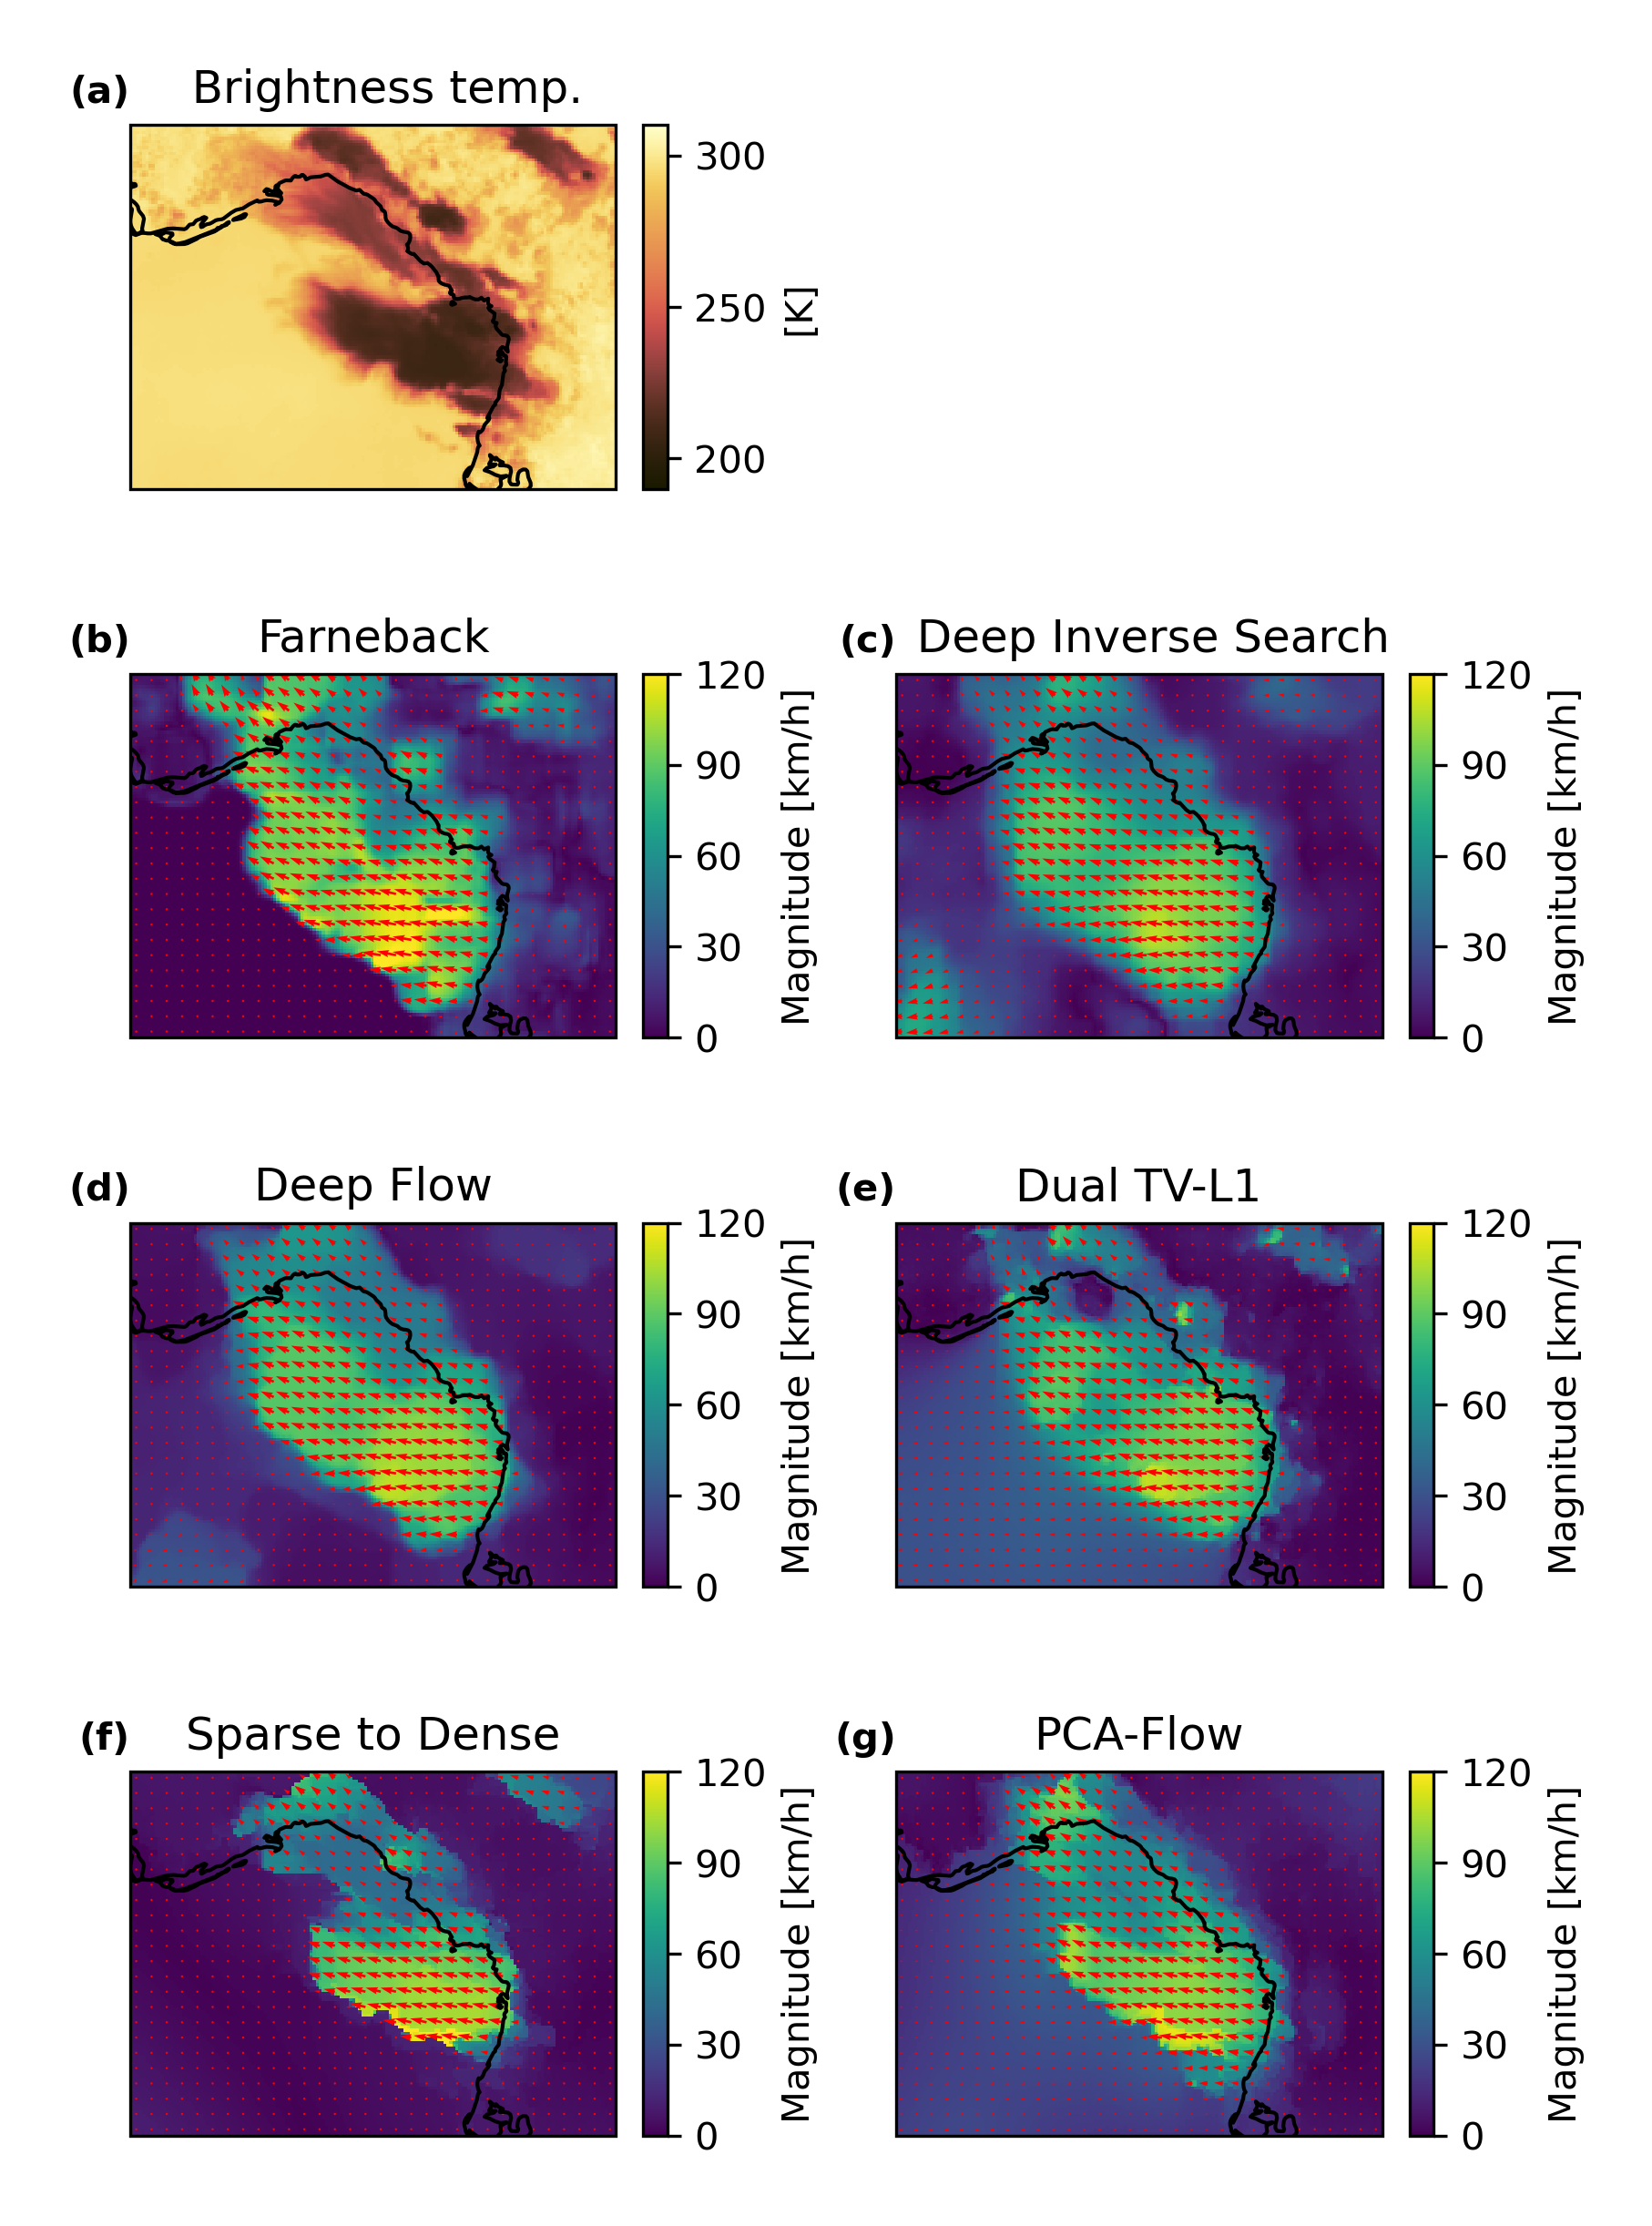
\includegraphics[width=0.9\textwidth]{figures/chapter1_10.png}
    \caption[
    A comparison of the motion vector fields generated by different optical flow methods
    ]{
    A comparison of the motion vector fields generated by the (b) Farnebäck, (c) \acrshort{dis}, (d) DeepFlow, (e) \acrshort{dualtvl1}, (f) Sparse to Dense, and (g) \acrshort{pca}-Flow. Optical flow vectors shown are estimated between the 10.4\,\unit{\mu m} channel at 19:00:00 \acrshort{utc} (a) and the subsequent image. Red arrows (b--g) show the motion vectors averaged over each 5\texttimes 5-pixel area is plotted by the red arrows, and the background shows the magnitude of the velocity vectors.
    }
    \label{fig:opt_flow_comparison}
\end{figure}


Figure~\ref{fig:opt_flow_differences} shows the difference in \acrshort{bt} between subsequent observations when taking into account the cloud motion predicted by the different optical flow algorithms.
The plots are again shown for the time step at 19:00:00~\acrshort{utc}, with the 10.4\,\unit{\mu m} \acrshort{bt} at this time step shown again for reference in fig.~\ref{fig:opt_flow_differences}\,a.
Figure~\ref{fig:opt_flow_differences}\,b shows the Eulerian difference in \acrshort{bt}; the difference in the \acrshort{bt} observed at the same pixel locations on subsequent time steps.
We see large cooling rates of the left (downwind) side of the anvil cloud, not because the \acrshort{ctt} is cooling, but because of the expansion of the anvil cloud into previously cloud-free areas.
Separating these observations of cooling \acrshort{bt} caused by the motion and expansion of the anvil cloud from those due to the vertical growth of the \acrshort{dcc} is the main objective of the semi-Lagrangian approach.


\begin{figure}[tp]
    \centering
    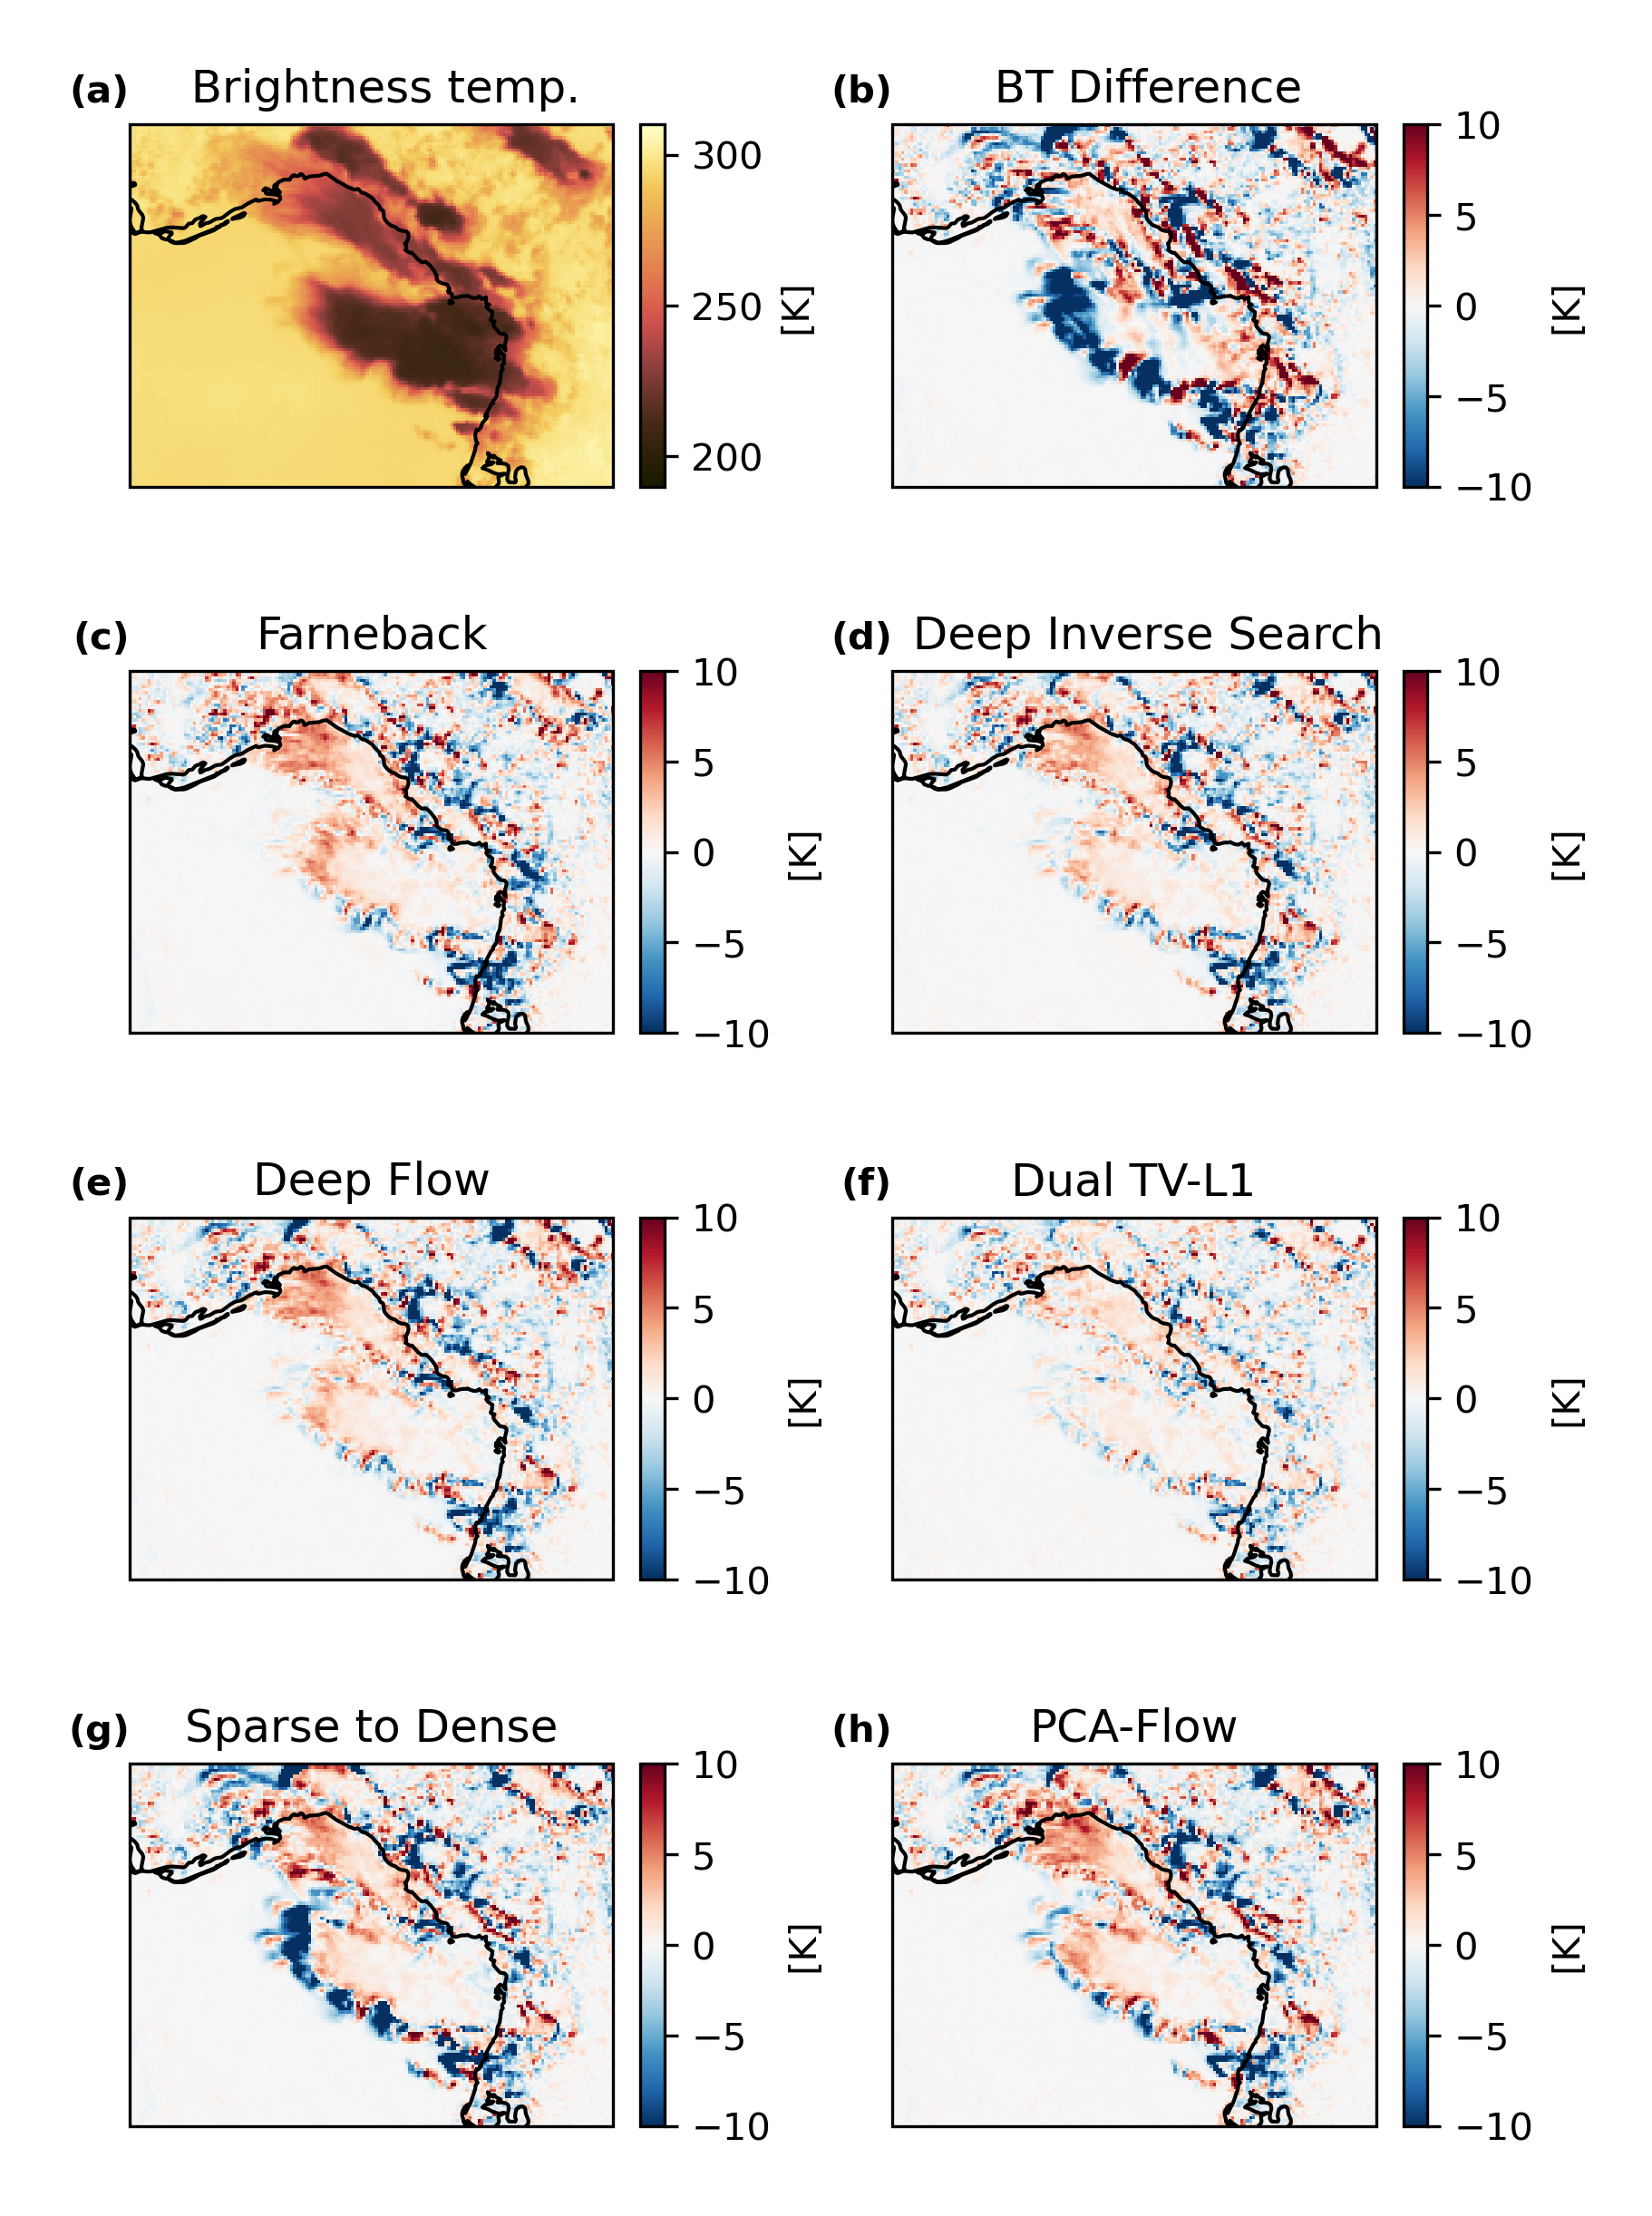
\includegraphics[width=0.9\textwidth]{figures/chapter1_11.png}
    \caption[
    The difference in \acrshort{bt} between subsequent \acrshort{abi} observations when taking into account the cloud motion predicted by the different optical flow algorithms.
    ]{
    The difference in \acrshort{bt} between subsequent \acrshort{abi} observations when taking into account the cloud motion predicted by the different optical flow algorithms. The plots are again shown for the time step at 19:00:00~\acrshort{utc}, with the 10.4\,\unit{\mu m} \acrshort{bt} at this time step shown for reference (a). b: the difference in \acrshort{bt} without accounting for cloud motion; c--h: the Lagrangian difference in \acrshort{bt} using motion vectors predicted by each of the optical flow algorithms.
    }
    \label{fig:opt_flow_differences}
\end{figure}


The dense optical flow methods (fig.~\ref{fig:opt_flow_differences}\,c--f) show good performance in removing the anomalous cooling observations seen downwind of the anvil cloud.
The Farnebäck, \acrshort{dis} and DeepFlow algorithms (fig.~\ref{fig:opt_flow_differences}\,c--e) all show a warming tendency towards the edge of the anvil cloud.
Although this may be explained by an overestimation of the cloud motion by these algorithms, this may also be a real observation of apparent warming due to thinning of the detraining anvil cloud.
The \acrshort{dualtvl1} algorithm (fig.~\ref{fig:opt_flow_differences}\,f) shows generally smaller differences than the other algorithms.
This is likely due to the algorithm accounting for changes in brightness between observations, whereas the other algorithms assume that the brightness of tracked objects remains constant between observations.

The two sparse optical flow algorithms (fig.~\ref{fig:opt_flow_differences}\,g,h) both show worse performance, with the sparse to dense method performing particularly poorly.
Both algorithms show cooling downwind of the anvil, likely because the region-based methods used to map the sparse motion vectors to the whole image do not detect this region well.

\begin{figure}[tp]
    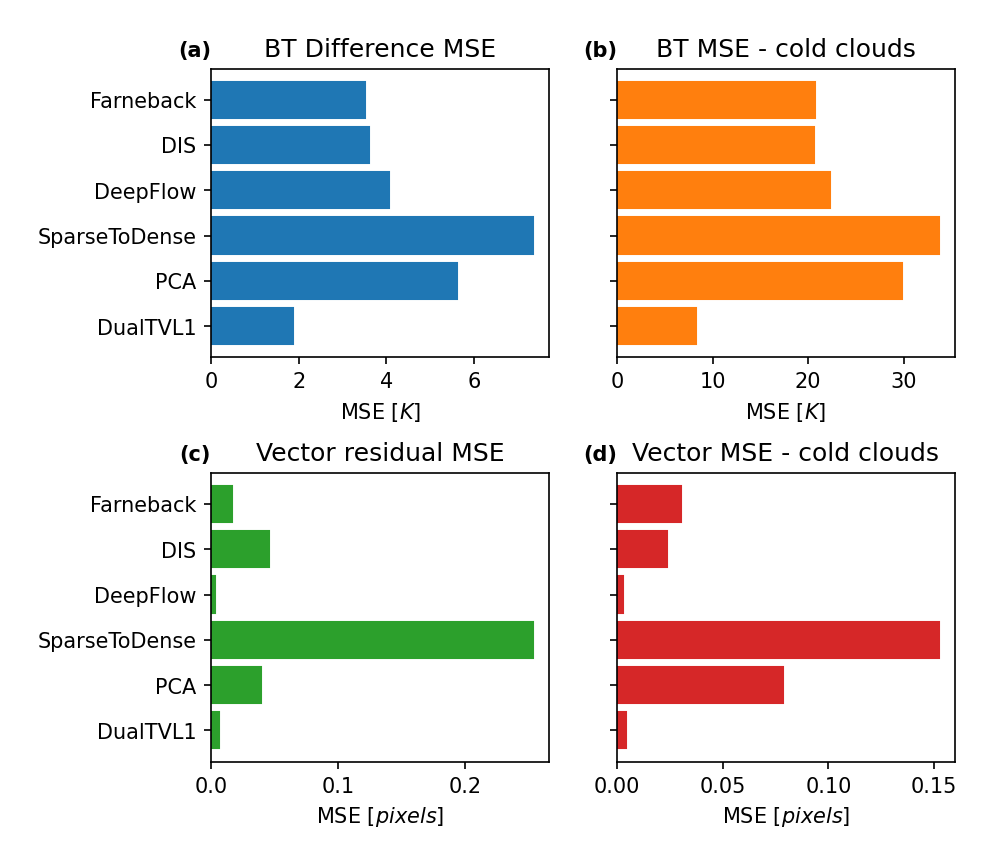
\includegraphics[width=0.9\textwidth]{figures/chapter1_12.png}
    \caption[
    A comparison of the \acrshort{bt} difference and residual vector magnitude \acrshort{rmse} for each of the optical flow algorithms
    ]{
    A comparison of the \acrshort{rmse} for each of the optical flow algorithms. a: \acrshort{bt} difference \acrshort{rmse} for all pixels and (b) for pixels with \acrshort{bt} $<$ 273\,\unit{K}. c: \acrshort{rmse} of the residual vector magnitude for all pixels and (d) for pixels with \acrshort{bt} $<$ 273\,\unit{K}.
    }
    \label{fig:opt_flow_mse}
\end{figure}

Figure~\ref{fig:opt_flow_mse}\,a shows the \acrfull{rmse} of the \acrshort{bt} differences shown in fig.~\ref{fig:opt_flow_differences} for each algorithm.
As seen in fig.~\ref{fig:opt_flow_differences}, the \acrshort{dualtvl1} algorithm has the smallest differences, the other dense algorithms perform similarly, and the \acrshort{pca}-Flow and sparse to dense algorithms perform the worst.
It should be noted that we should expect some differences in the \acrshort{bt} due to actual changes in the \acrshort{ctt}.
Figure~\ref{fig:opt_flow_mse}\,b shows the \acrshort{rmse} of the \acrshort{bt} differences for pixels with \acrshort{bt} less than 273\,\unit{K}, representing cold cloud observations.
While the \acrshort{rmse} shown here for all algorithms is large compared to the sensor noise previously calculated for the \acrshort{bt} difference in section~\ref{sec:theory_core} (0.47\,K), it should be noted that some of the \acrshort{rmse} here is due to contributions from changes in the height of the anvil cloud.
As a result, the actual error in the \acrshort{bt} difference over time due to horizontal cloud motions not captured by the optical flow algorithm is likely much smaller, on a similar magnitude to the \acrshort{nedt}.

To estimate the uncertainty in the calculated motion vectors, we calculate the residual motion vectors for each algorithm.
The residual motion is calculated by first warping each image to the locations predicted by the optical flow vectors, in the same manner used to calculate the \acrshort{bt} differences in fig.~\ref{fig:opt_flow_differences}.
Then the optical flow algorithms are used to calculate a second set of residual vectors between each image and the subsequent warped image.
In theory, if the initial motion vectors were calculated perfectly, warping the image by the optical flow vectors should result in the subsequent cloud in the same position as the prior image, and so the second set of motion vectors should calculate as zero.
The magnitude of the residual motion vectors is therefore considered as the uncertainty in the initial set of motion vectors.

Figure~\ref{fig:opt_flow_mse}\,c,d show the \acrshort{rmse} of the residual vector magnitudes for all pixels and pixels less than 273\,\unit{K} respectively.
The DeepFlow and \acrshort{dualtvl1} algorithms again show the best accuracy, and sparse to dense the worst.
The Farnebäck algorithm shows good accuracy across all pixels, as seen in the ability to correctly detect zero motion in cloudless skies in fig.~\ref{fig:opt_flow_comparison}.
However, when considering only cold pixels the Farnebäck algorithm performs slightly worse than \acrshort{dis}.

The results shown in fig.~\ref{fig:opt_flow_mse} suggest that the \acrshort{dualtvl1} algorithm is the best choice for estimating the motion vectors in satellite observations of \acrshort{dcc}.
However, due to the large size and long sequences of images produced by \acrshort{abi}, it is also important to consider the computational cost of each algorithm.
Figure~\ref{fig:opt_flow_cost} shows the run time in seconds for each algorithm applied to a sequence of 48 300\texttimes300~pixel \acrshort{abi} \acrshort{bt} images.
Both the DeepFlow and \acrshort{dualtvl1} algorithms show significantly longer run times than any of the other algorithms.
As a result, we have selected the Farnebäck algorithm for our tracking method as it offers the best balance of accuracy and computational performance for running on large datasets.


\begin{figure}[tp]
    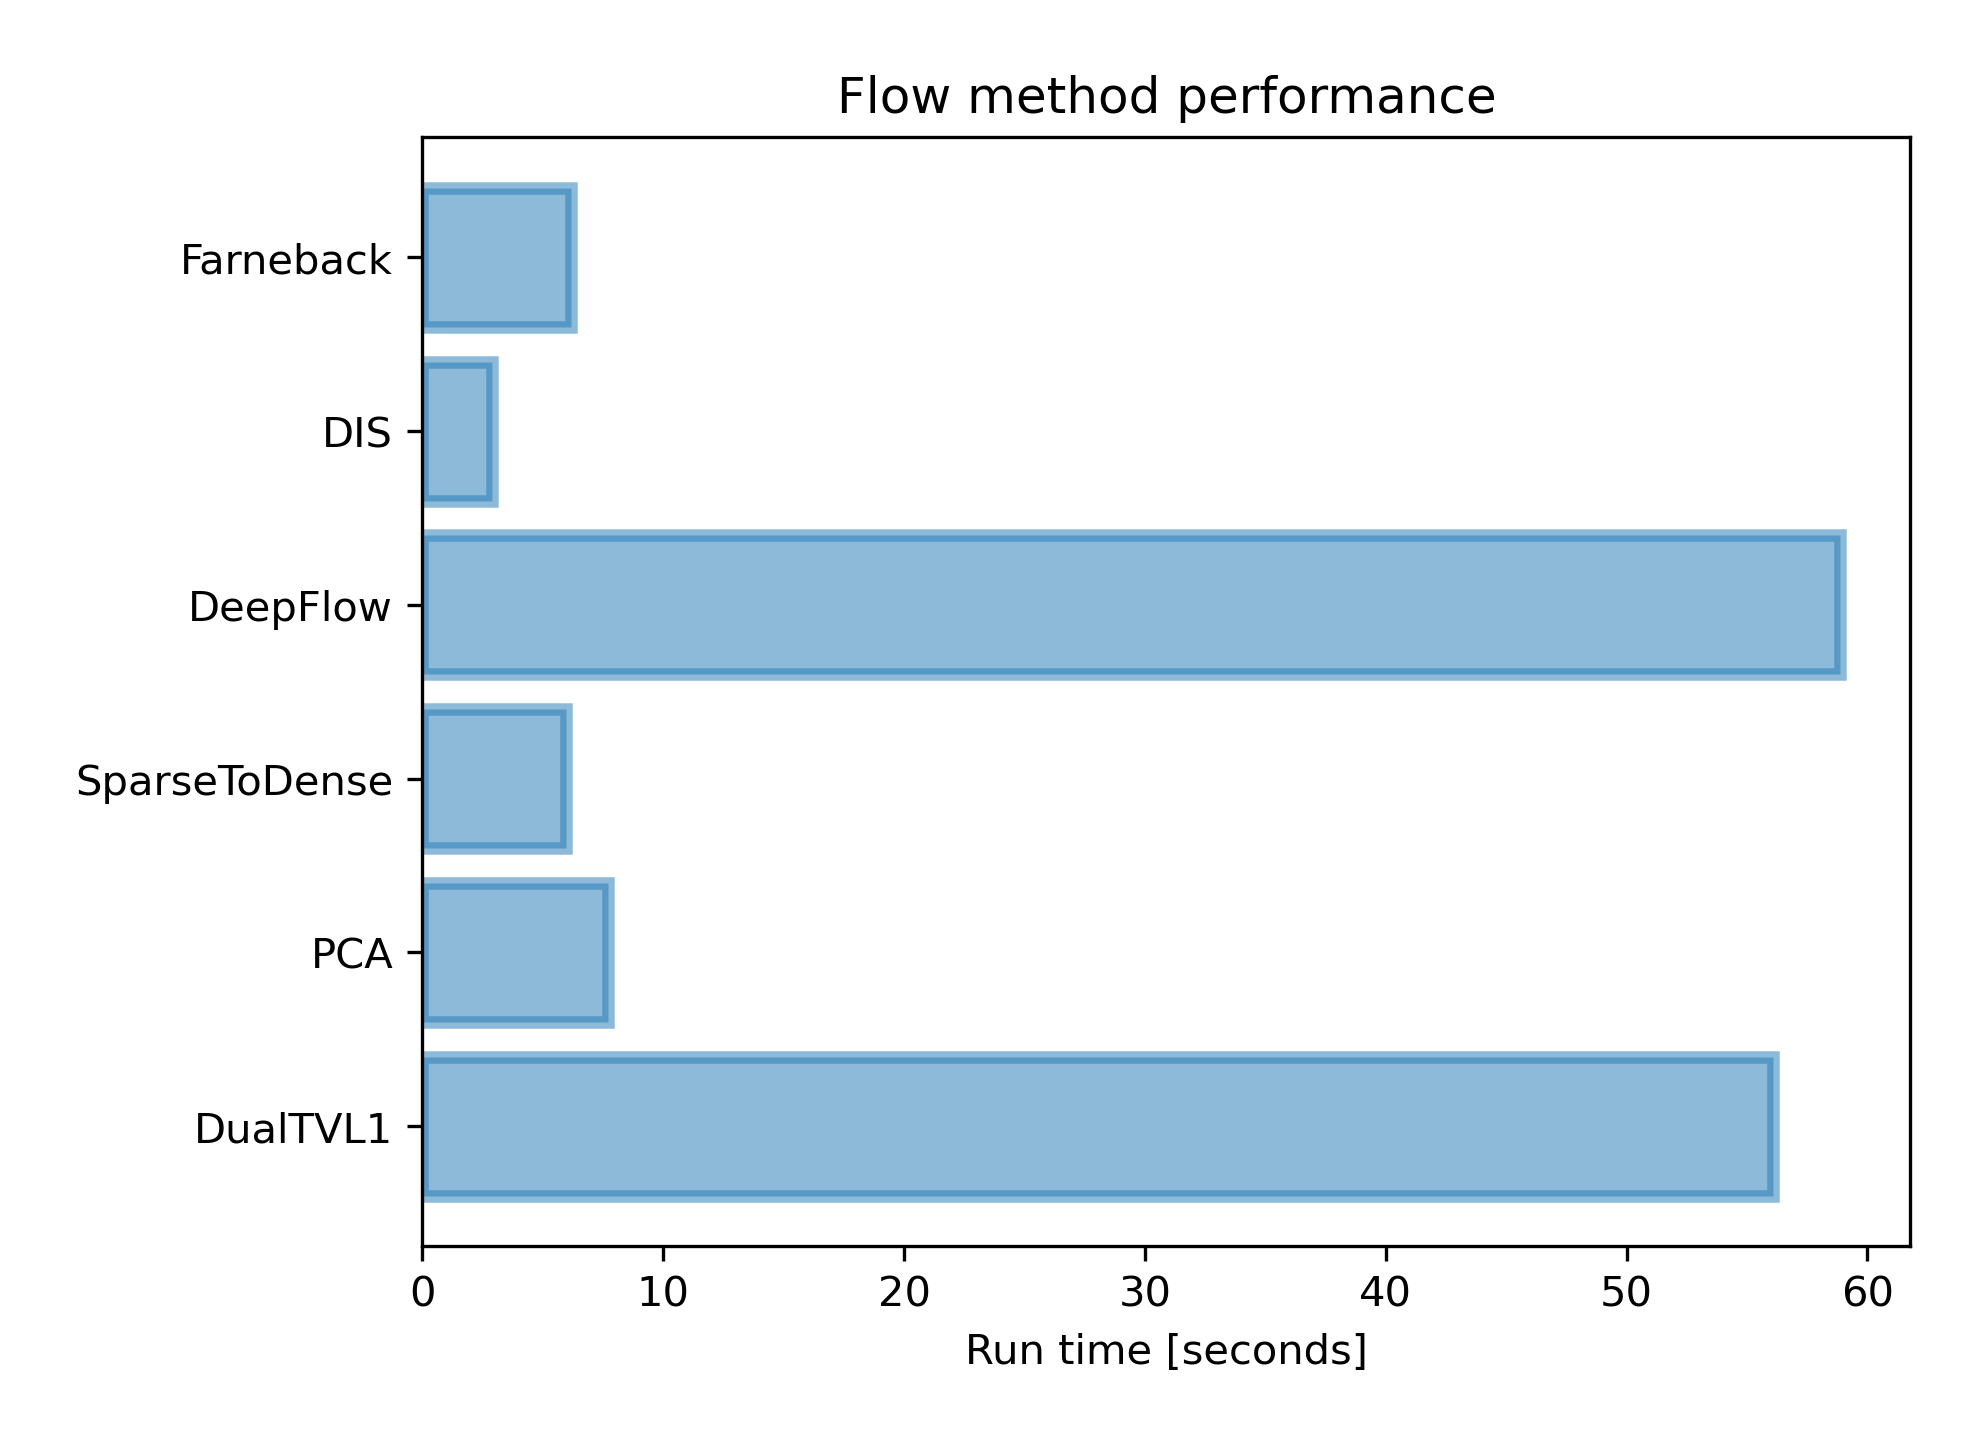
\includegraphics[width=0.9\textwidth]{figures/chapter1_13.png}
    \caption[
    A comparison of the computational performance of each optical flow method
    ]{
    A comparison of the computational performance of each optical flow method. Run-time was measured for a sequence of 48 300\texttimes300 pixel \acrshort{abi} 10.4\,\unit{\mu m} \acrshort{bt} images.
    }
    \label{fig:opt_flow_cost}
\end{figure}


An example of the motion vectors calculated by the Farnebäck algorithm when applied to the 10.4\,\unit{\mu m} \acrshort{bt} field is shown in fig.~\ref{fig:optical_flow}.
Figure~\ref{fig:optical_flow}\,c shows the residual flow vectors, which are small compared to the detected cloud motion vectors (fig.~\ref{fig:optical_flow}\,b).
The main areas in which residual flow vectors can be seen are the regions around the edge of anvil clouds and in the centre of thick anvil clouds where there are no clear features to track.
Figure~\ref{fig:optical_flow}\,d shows the distribution of residual vector errors proportional to the detected cloud motion vectors.
The majority of the residual errors are close to zero, and very few exceed 0.5.
As in the majority of applications for the semi-Lagrangian framework we are only interested in the motion to the nearest pixel, these errors are considered acceptable.


%f
\begin{figure}[tp]
    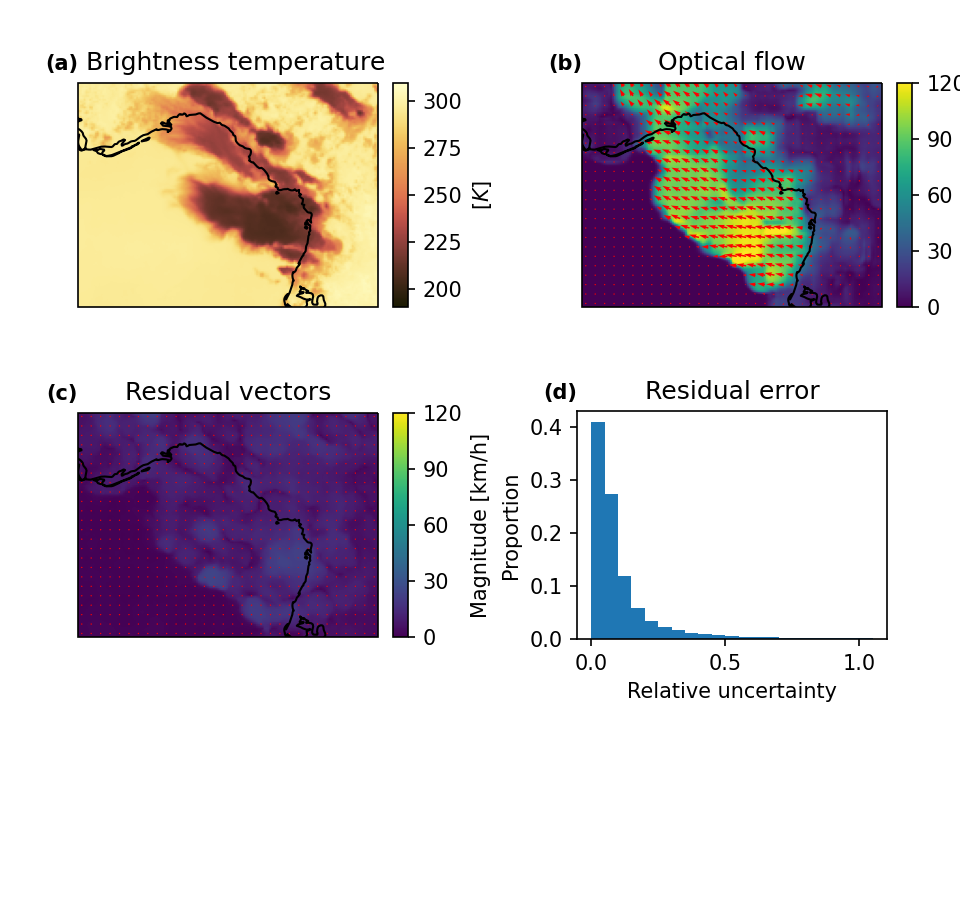
\includegraphics[width=\textwidth]{figures/chapter1_14.png}
    \caption[
    An example of the motion vectors and their residual errors calculated using the Farnebäck algorithm
    ]{
    An example of the motion vectors and their residual errors calculated using the Farnebäck algorithm. a: the 10.4\,\unit{\mu m} \acrshort{bt} field at 19:00:00~\acrshort{utc} for which the motion vectors are shown. b: the calculated motion vectors. c: the residual motion vectors, indicating the uncertainty in the optical flow. d: the magnitude of the residual motion vectors as a proportion of the magnitude of the optical flow vectors for cold pixels (less than 273\,\unit{K})
    }
    \label{fig:optical_flow}
\end{figure}


Two potential sources of uncertainty are the assumptions made by the Farnebäck algorithm that the feature being tracked remains the same size and intensity in subsequent images.
For optical flow tracking using \acrshort{bt} images of growing \acrshort{dcc}s, neither of these assumptions are true.
However, we have taken steps to reduce the impact of both these sources of uncertainty on the tracking algorithm.
For the first of these assumptions, we find that in the case of small, fast-moving \acrshort{dcc}s -- where the accuracy of the optical flow vectors is most important -- the changes in the size of the \acrshort{dcc} is small compared to the overall motion, and so the uncertainty introduced is small.
Comparably, for large \acrshort{dcc}s where the changes in size may be large compared to the motion, the uncertainty has less impact on the tracking algorithm.
In the worst-case scenario, the estimated optical flow field will be zero, in which case the "3D" detection and tracking algorithm works in the same manner as that of \citet{fiolleau_algorithm_2013}, which is suitable for use on these larger \acrshort{dcc}s.

\subsection{A Semi-Lagrangian Framework for Morphological Image Processing}

Morphological image operations analyse images using their geometrical and structural properties.
Core to many morphological algorithms, from simple filters to complex neural networks \citep{kalchbrenner_convolutional_2014}, is the kernel, or convolution method.
A convolution method performs operations on the pixels of an image by applying a convolution stencil to the pixel and its neighbours.
In a conventional convolution scheme, such as that used in the methods of \citet{fiolleau_algorithm_2013}, the convolution stencil acts on adjacent pixels in both time and space (see fig.~\ref{fig:convolution_kernels}\,a).
In this Eulerian framework, different locations in time are considered in the same manner as those in the spatial dimensions.
However, we know from previous analysis of \acrshort{dcc}s that the motion of convective cores between images can be similar to the spacing of cores and their size \citep{heikenfeld_tobac_2019}.
As a result, it is important to include the effects of advection when comparing images across time steps.


%f
\begin{figure}[tp]
    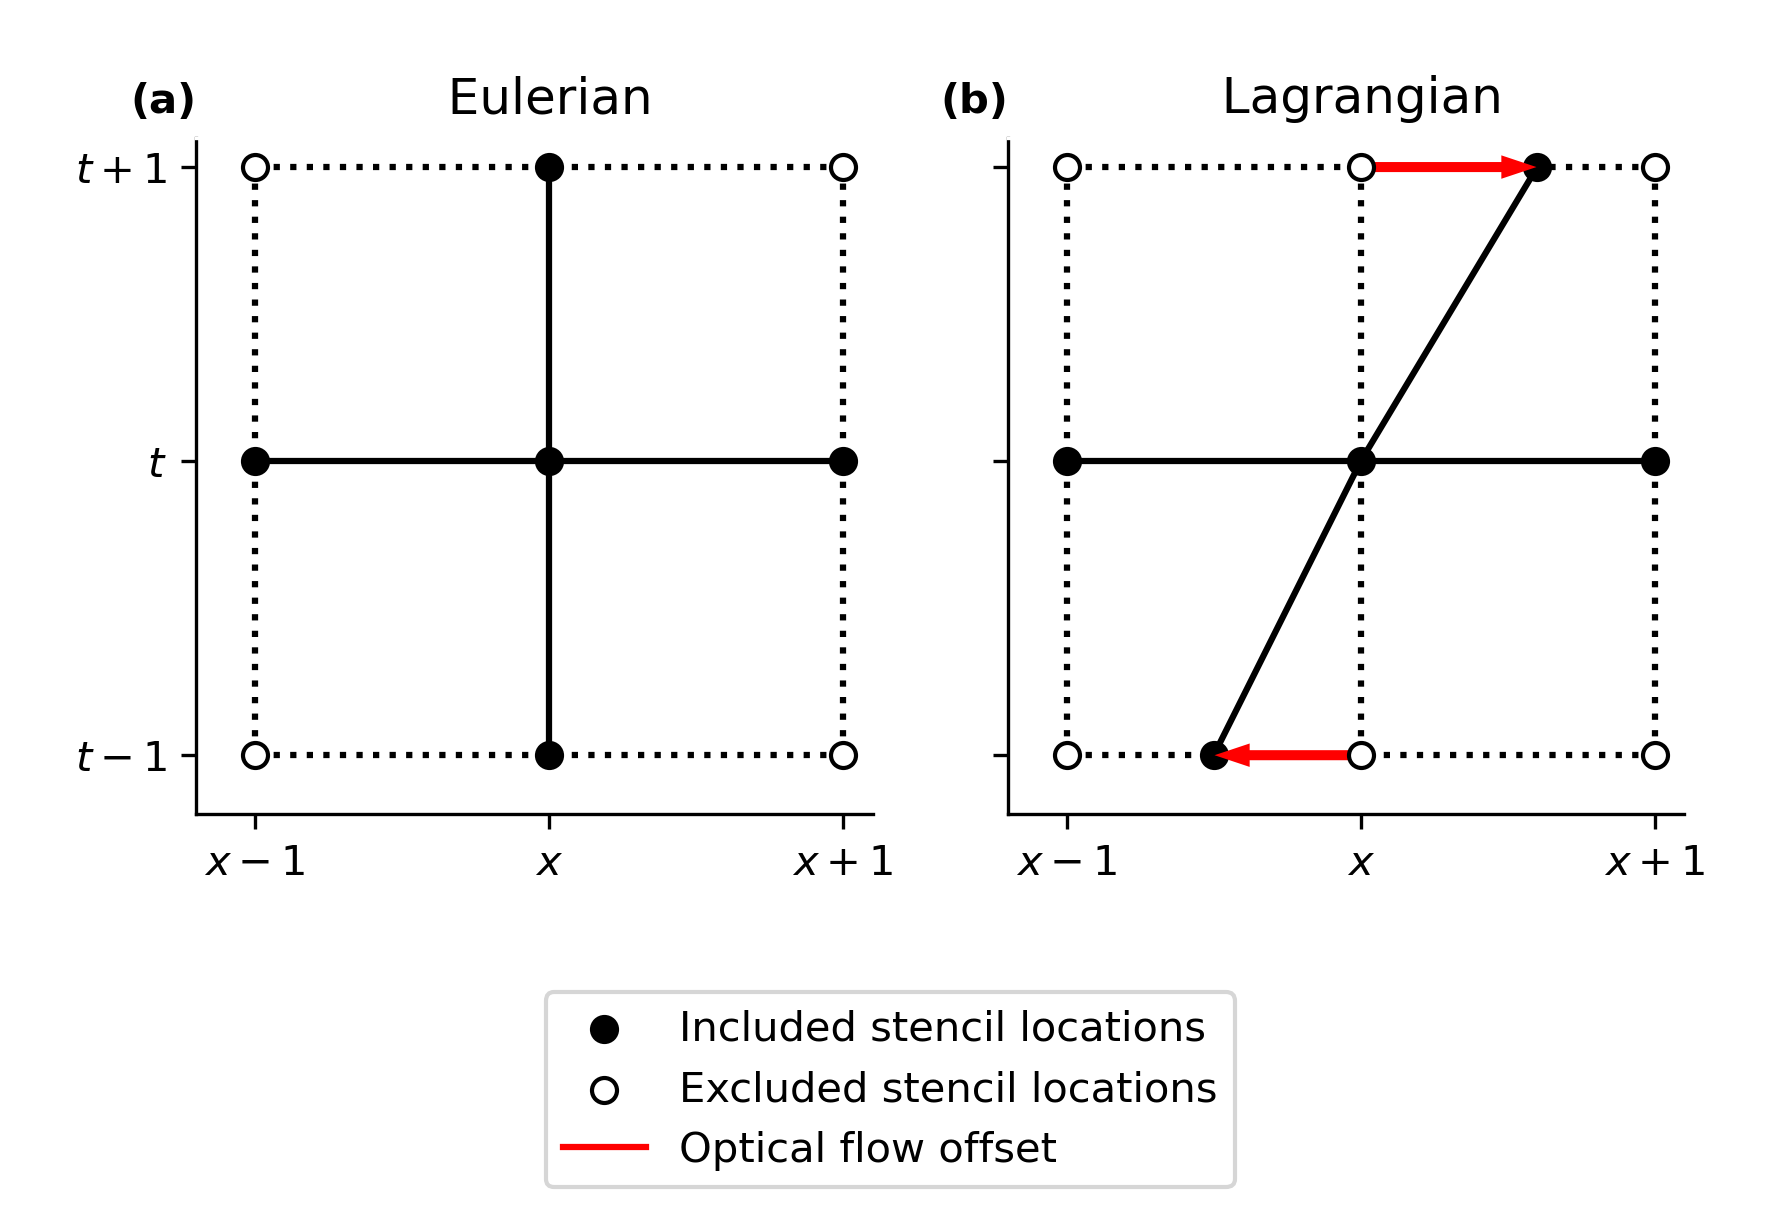
\includegraphics[width=0.75\textwidth]{figures/chapter1_15.png}
    \caption[
    A comparison of convolution stencils with square connectivity in Eulerian and Lagrangian frameworks.
    ]{
    A comparison of convolution stencils with square connectivity in Eulerian (a) and Lagrangian (b) frameworks. In the Lagrangian framework, the points at prior and subsequent time steps are offset by the calculated optical flow field.
    }
    \label{fig:convolution_kernels}
\end{figure}


To perform morphological operations which take into account this advection, we have developed a novel Lagrangian convolution method.
For spatial operations, the Lagrangian stencil operates identically to that of a classical convolution method.
However, when sampling points at prior or subsequent time steps, the location of the stencil points are offset by the relevant optical flow vectors (fig.~\ref{fig:convolution_kernels}\,b).
Values at the offset stencil locations are interpolated, providing a Lagrangian reference frame for changes in the observations over time.
Applying the convolution stencil to every pixel in a sequence of images provides a semi-Lagrangian framework for morphological operations, combining the Lagrangian reference frame for evaluating changes over time while maintaining the regular grid of the images.

We have developed new implementations of several existing image processing operations within the Lagrangian convolution framework, including:
\begin{itemize}
    \item Sobel edge detection \citep{sobel_isotropic_2014}
    \item Watershed segmentation using the connected-components method \citep{bieniek_efficient_2000}
    \item Labelling of connected components \citep{hoshen_percolation_1976}
\end{itemize}

These operations are used in this method to detect the full extent of the anvil cloud associated with the \acrshort{dcc}, to perform detection continuously across multiple time periods while accounting for the motion of the \acrshort{dcc}, and to identify individual \acrshort{dcc}s and \acrshort{dcc} clusters across multiple time periods respectively.

The Sobel method detects edges in an image using the magnitude of the local gradient at each pixel.
Edge detection enables the segmentation of an image into separate regions without pre-defined thresholds (such as in \acrshort{bt}) to separate them.

Watershed algorithms are a method of image segmentation that equates an image to a topographical map, with elevation according to the value of the pixel.
Each pixel is then descended towards its local minima until it reaches a predefined marker region.
The method takes its name from the geographical feature of the same name, which refers to the separation between adjacent drainage basins.
Although this physical interpretation of the algorithm applies to two-dimensional images, the method can be applied to arrays with any number of dimensions, such as the method used by \citet{fiolleau_algorithm_2013} which applied watershedding to a three-dimensional field.

Labelling algorithms assign unique identifiers to each segmented region provided by either the edge detection or watershed algorithms.


\subsection{Detection of Growing Deep Convection} \label{sec:core_detection}

Growing deep convective cores are detected in a similar manner to that used by \citet{zinner_cb-tram_2008}.
The growth rates are calculated using the finite difference of the 10.4\,\unit{\mu m } \acrshort{bt} and \acrshort{wvd} fields in the Lagrangian perspective.
We have found that combining both the 10.4\,\unit{\mu m} \acrshort{bt} and the \acrshort{wvd} field provides the best observations for detecting growing deep convective cores.
The \acrshort{bt} field shows cooling cloud tops throughout the troposphere, while the \acrshort{wvd} isolates growth in the mid- to upper-troposphere, removing spurious observations of growth due to boundary layer convection and cloud formation.

We classify a region of growing deep convection as a region of either continuous cooling of greater than 0.5\,\unit{K} per minute in the 10.4\,\unit{\mu m} \acrshort{bt} field, or continuous warming of the \acrshort{wvd} field of at least 0.25\,\unit{K} per minute.
These growth rates must be detected over a minimum 15-minute period, covering an area of at least 3 by 3 pixels (approximately 7.5 by 7.5\,\unit{km}) at each time step.
Each region of detected growth is given a unique label, the average \acrshort{bt} of the detected cloud at each time step is calculated, and any label which fails to meet the cooling rate thresholds of 8\,\unit{K} over a 15-minute period (from \citep{roberts_nowcasting_2003, hartung_intercomparison_2013}) are removed.
Finally, each label is checked to ensure that the growth region ends with a \acrshort{wvd} field with a value of greater than -5, indicating that the growing core reaches a high altitude \citep{muller_role_2018}.
While threshold detection methods are sensitive to noise, the uncertainty in the \acrshort{bt} cooling rates due to sensor noise, combined with the uncertainty in the optical flow vectors, is not expected to exceed 5\% of the threshold.
A simple threshold method applied to the \acrshort{bt} cooling rate is, therefore, suitable for the detection of developing deep convection.

Figure~\ref{fig:core_detection} shows a comparison between the detected core cooling rates in \acrshort{abi} imagery and the corresponding column radar reflectivity measured by \acrshort{nexrad} for the case of newly developing convection (fig.~\ref{fig:core_detection}\,a,c,e) and mature \acrshort{dcc} (fig.~\ref{fig:core_detection}\,b,d,f)
Both 10.4\,\unit{\mu m} \acrshort{bt} and \acrshort{wvd} growth rates show growth detected in the same locations as the high column radar reflectivity from \acrshort{nexrad}.
As predicted by the results in section~\ref{sec:theory_core}, the observed growth rates in the \acrshort{wvd} are about half of those in the 10.4\,\unit{\mu m} \acrshort{bt}.


%f
\begin{figure}[tp]
    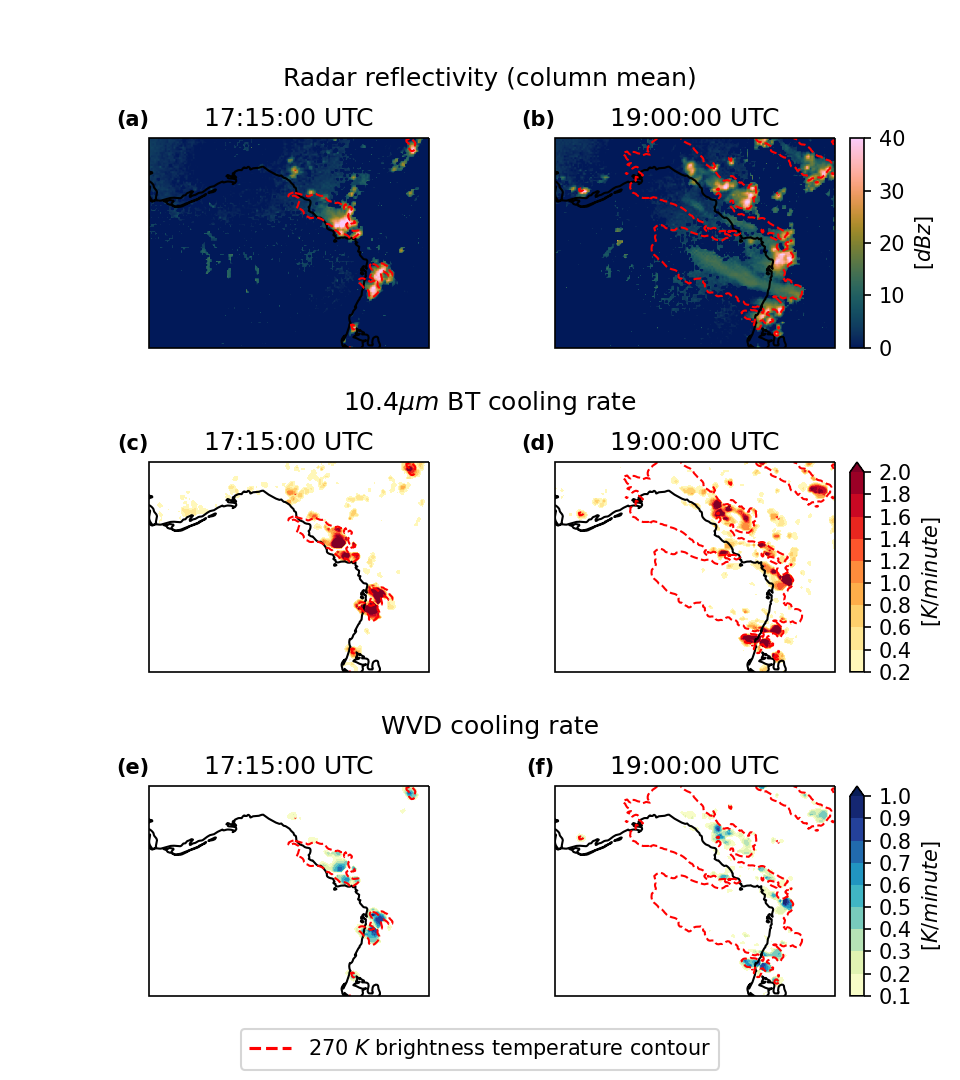
\includegraphics[width=\textwidth]{figures/chapter1_16.png}
    \caption[
    Detection of growing \acrshort{dcc} using \acrshort{nexrad} column radar reflectivity, 10.4\,\unit{\mu m} \acrshort{bt} and \acrshort{wvd} growth rates
    ]{
    Detection of growing \acrshort{dcc} regions for the \acrshort{dcc} cluster in figure~\ref{fig:compare_sat_radar_glm}. a,b: \acrshort{nexrad} column mean radar reflectivity remapped to the \acrshort{abi} grid. c,d: cooling rate of the 10.4\,\unit{\mu m} \acrshort{bt} field. e,f: warming rate of the \acrshort{wvd} field.
    }
    \label{fig:core_detection}
\end{figure}


Both 10.4\,\unit{\mu m} and \acrshort{wvd} growth rates in the growing phase (fig.~\ref{fig:core_detection}\,c,e) show good agreement with column radar reflectivity (fig.~\ref{fig:core_detection}\,a).
However, during the mature stage of the \acrshort{dcc}, discrepancies develop between the observed growth rates (fig.\ref{fig:core_detection}\,d,f) and the radar reflectivity (fig.~\ref{fig:core_detection}\,b) due to the development of the anvil cloud blocking satellite observations of the core underneath.


\subsection{Detection of Anvil Clouds} \label{sec:anvil_detection}

The region of anvil cloud associated with the growing convective clouds detected in section \ref{sec:core_detection} is detected and tracked using an edge-based watershed segmentation approach.
The edge-based approach to cloud detection avoids the use of a fixed threshold for anvil temperature, and so can detect a more accurate extent of the anvil cloud \citep{dim_alternative_2013}.
We define an upper threshold for the \acrshort{wvd} field of -5\,\unit{K}, as used by \citet{muller_role_2018}, and a lower threshold of -12.5\,\unit{K}, which we define as definite non-anvil cloud.
Because the presence of thin cirrus outflow from the anvil clouds can make it difficult to determine the extent of the anvil cloud, we use the \acrshort{swd} field as described in section 2.1 to either remove or include the region of cirrus outflow in the detected anvil region.
To detect the thick anvil cloud, we subtract the \acrshort{swd} field (fig.~\ref{fig:edge_detection}\,a).
In this case, the upper and lower thresholds remain the same as the \acrshort{swd} field is approximately 0~K for thick, high clouds, and so has no effect on the temperature of these features.
For detecting the thin anvil region, we add the \acrshort{swd} field and increase the value of both thresholds by 5\,\unit{K} to 0\,\unit{K} and -7.5\,\unit{K} respectively (fig.~\ref{fig:edge_detection}\,c).
This change is made to account for the effect of low-level \acrshort{wv} on the \acrshort{swd} field which gives a background value of approximately 5~K.
Between these two thresholds, we have a region in which we are uncertain of the extent of the anvil cloud.
By applying a Sobel filter to detect the local gradient magnitude of the combined \acrshort{wvd}/\acrshort{swd} field \citep{sobel_isotropic_2014}, we detect the outer extent of the anvil cloud within this region where we see the greatest magnitude in the detected edges (see fig.~\ref{fig:edge_detection}\,b,d).

The uncertainty due to sensor noise is small relative to the range between the two thresholds, at 2.7\,\% for the combined \acrshort{wvd} and \acrshort{swd} fields.
While this low noise may indicate that a simple threshold approach may be suitable, such an approach would be susceptible to the systematic biases in the \acrshort{wvd} and \acrshort{swd} observations identified in section~\ref{sec:abi_channels}.
Combining the edge detection approach with the two-threshold approach provides robustness to systematic bias, since as long as the maximum gradient of the cloud edge remains between the two thresholds the same cloud extent should be detected.
This allows systematic biases on the order of several K without significantly affecting the results, allowing better comparison of \acrshort{dcc}s observed in different environments.


%f
\begin{figure}[tp]
    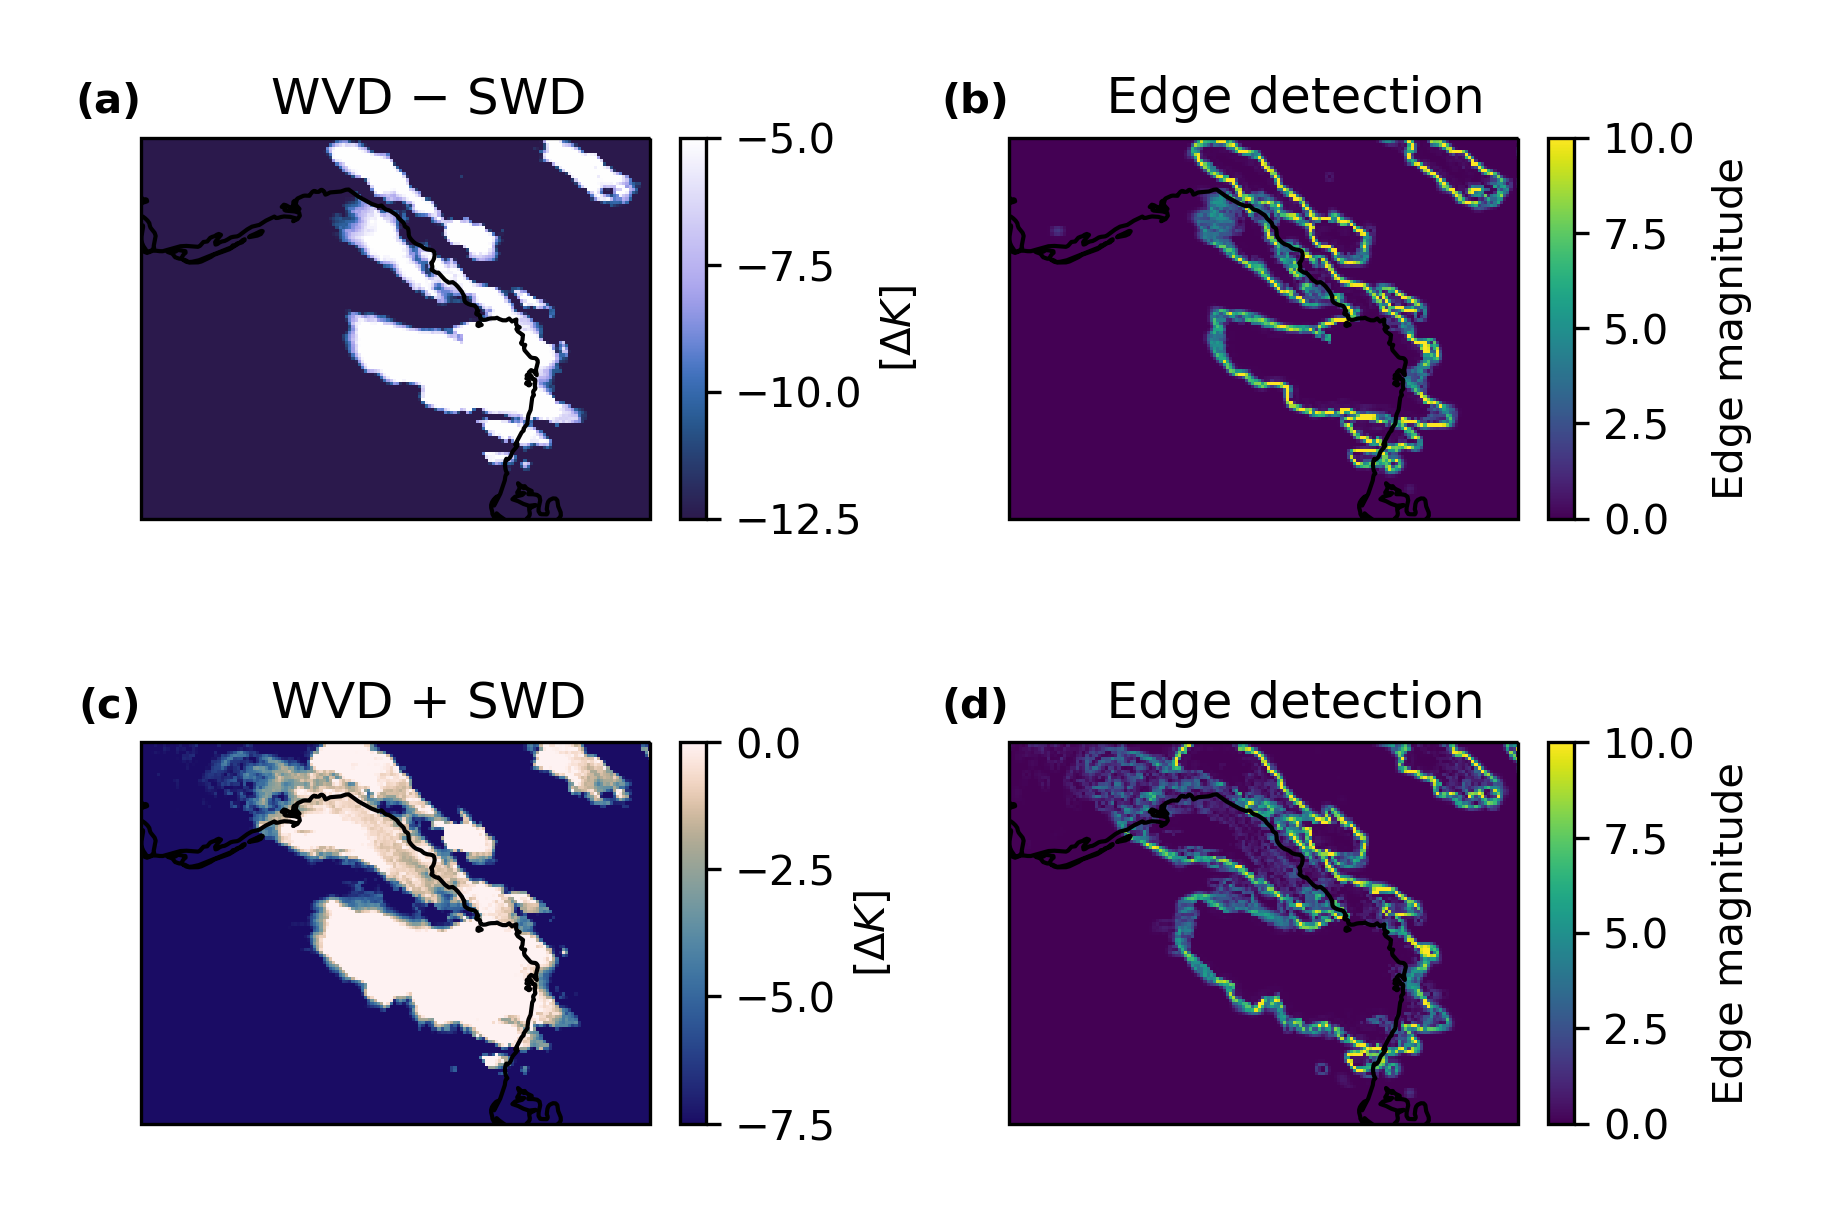
\includegraphics[width=\textwidth]{figures/chapter1_17.png}
    \caption[
    Detection of anvil cloud extent for the mature \acrshort{dcc} cluster in \ref{fig:compare_sat_radar_glm} using the edge gradient method
    ]{
    Detection of anvil cloud extent for the mature \acrshort{dcc} cluster in \ref{fig:compare_sat_radar_glm} using the edge gradient method. a.: The combined field of the \acrshort{wvd} minus the \acrshort{swd}, to isolate the thick anvil, between the upper and lower thresholds of -5 and -12.5\,\unit{K} respectively. b.: the detected edge gradient magnitude of the field between these thresholds, which is used to detect the outer extent of the thick anvil cloud. c.: the combined field of \acrshort{wvd} plus the \acrshort{swd}, to enhance the thin anvil, and d.: the calculated edge magnitude of this field.
    }
    \label{fig:edge_detection}
\end{figure}


When applied to the detected edges of the anvil clouds using the Sobel filter, with the growth regions detected previously as markers, the watershed method allows us to detect those anvil regions associated with detected regions of growing \acrshort{dcc}s, while avoiding the detection of non-convective regions of high, cold clouds.
Furthermore, due to the application of the watershed algorithm to both the spatial and temporal dimensions of the sequence of images through the semi-Lagrangian framework, we are able to detect the associated anvil clouds after the growth of the \acrshort{dcc} is no longer observed.


Figure~\ref{fig:detected_anvils} shows an example of the results of detecting and tracking \acrshort{dcc} cores (outlined in red) and the associated anvils (outlined in orange and blue for the thick and thin anvil regions respectively).
During the growing phase (fig.~\ref{fig:detected_anvils}\,a,b) we see a number of developing cores, as well as the initial growth of primarily thick anvil cloud.
In fig.~\ref{fig:detected_anvils}\,c--e we see the mature phase of the \acrshort{dcc}, where we see the thick anvil expand and the thin anvil cirrus start to detrain towards the top-left side of the figure.
Due to the anvil cloud reaching its maximum height, we no longer observed the initial developing cores seen in fig.~\ref{fig:detected_anvils}\,a,b as we can no longer observe the cloud-top cooling.
Instead, we observe new cores developing on the edges of the anvil cloud.
In fig.~\ref{fig:detected_anvils}\,f--h, we see the detected anvil cloud beginning to dissipate.
The thick anvil area decreases, however the thin anvil area continues to increase as the anvil dissipates and detrains.
At this point in the lifetime of the tracked \acrshort{dcc} we stop observing new growing cores, however the "3D" approach allows the continued tracking of the anvil cloud until it dissipates.


%f
\begin{figure}[tp]
    \centering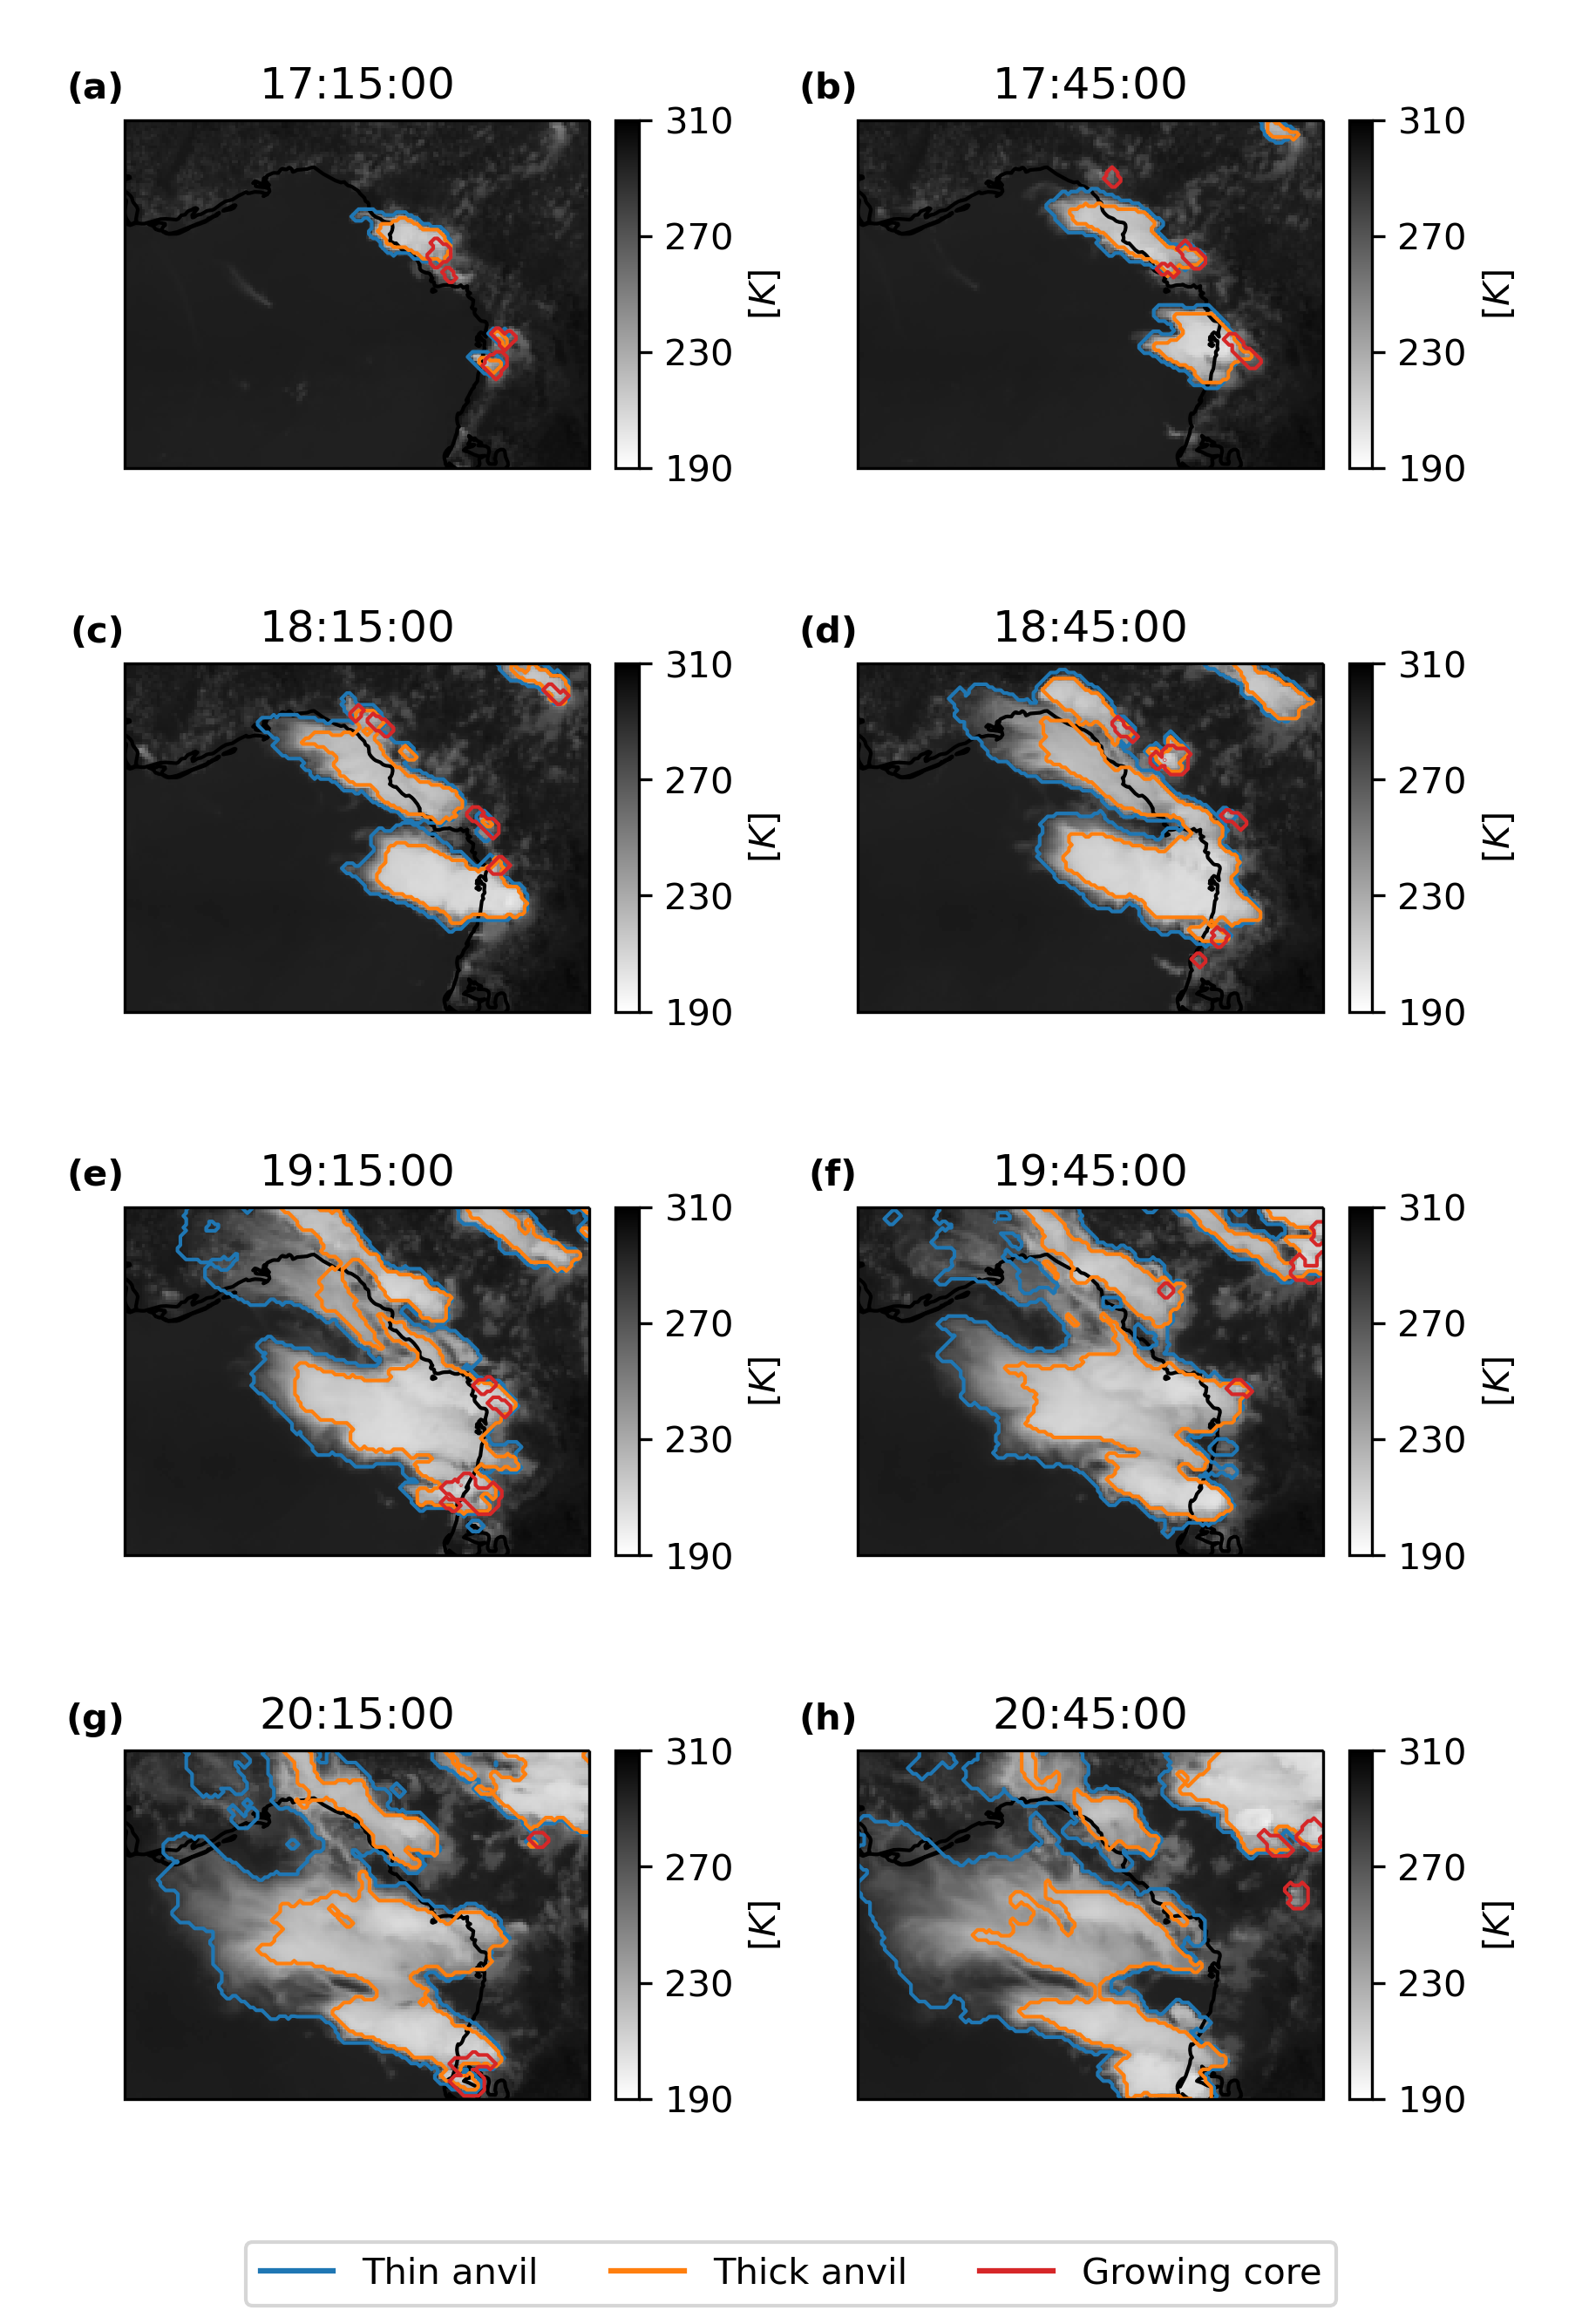
\includegraphics[width=0.8\textwidth]{figures/chapter1_18.png}
    \caption[
    Detected regions of thin anvil cloud, thick anvil cloud, and developing cores through the growing, mature and dissipating phases of the \acrshort{dcc} lifecycle
    ]{
    Detected regions of thin anvil cloud (blue), thick anvil cloud (orange), and developing cores (red) overlaid on the \acrshort{goes}-16 \acrshort{abi} 10.4\,\unit{\mu m} \acrshort{bt} field for the \acrshort{dcc} cluster from figure~\ref{fig:compare_sat_radar_glm}. The three stages of the \acrshort{dcc} lifecycle are shown; the growth phase (a,b), the mature phase (c--e), and the dissipating phase (f--g).
    }
    \label{fig:detected_anvils}
\end{figure}


\section{Evaluation}


The effectiveness of the semi-Lagrangian framework for the detection of \acrshort{dcc}s is evaluated by analysing the proximity of detected anvil cloud regions to lightning flash detection from \acrshort{glm}.
Lightning observations are frequently used to validate detection methods for deep convection \citep[e.g.][]{zinner_validation_2013, muller_novel_2019} due to the strong correlation between deep convective updraughts and lightning activity.
Although \acrshort{glm} is not capable of detecting all lightning events (approximately 70\% of lightning events are detected) \citep{peterson_removing_2020}, the high frequency of lightning flashes per \acrshort{dcc} mean that these observations provide a suitable ground truth for validation.
It should be noted that lightning observations are only suitable for validating the detection of the thick anvil region, as lightning does not occur in the cirrus outflow.
As a result, validation of the detection of the thin anvil region would require the use of other data such as cloud profiling radar or lidar observations, and is not considered further in this paper.


Here we apply the same validation method as used by \citet{muller_novel_2019} to evaluate the semi-Lagrangian framework for the detection of \acrshort{dcc}s.
We classify detection events into three categories:

\begin{itemize}
    \item Correct detection (CD), when the algorithm detects a \acrshort{dcc} that is collocated with one or more lightning observations
    \item False detection (FD), when the algorithm detects a \acrshort{dcc} but no lightning flash is observed
    \item Missed detection (ND), when the algorithm does not detect a \acrshort{dcc} but a lightning flash is observed
\end{itemize}

Using these three categories of events we can define two measures of accuracy for the detection of \acrshort{dcc}s.
The \acrfull{pod} is defined as the number of correct detections divided by the total number of correct and missed detections.
This provides a measure of how likely the algorithm is to detect a \acrshort{dcc} that exists in the ground truth.
The \acrfull{far} is defined as the number of false detections divided by the total number of correct and false detections.
This provides a measure of how likely a \acrshort{dcc} detected by the algorithm is not present in the ground truth.
The F\textsubscript{1}-score is calculated as the harmonic mean of the \acrshort{pod} and the recall (where the recall in is 1~\textminus~\acrshort{far}), and provides an overall measure of accuracy between 0 and 1.

When evaluating whether detected \acrshort{dcc} regions and lightning observations were collocated, \citet{muller_novel_2019} considered events within 32\,\unit{km} and 15 minutes to be collocated.
This margin of uncertainty was separated into two components, half from the physical separation between observed lightning strikes, and the remaining half from uncertainty in the collocation and geolocation of the satellite and lightning observations.
For a typical \acrshort{abi} pixel length over the \acrshort{conus} of 2-2.5\,\unit{km}, this margin of error translates into 15 pixels in the \acrshort{abi} view.
The distance between a \acrshort{glm} lightning flash and detected cloud region is defined as the distance between the flash and the nearest \acrshort{abi} pixel within that region, with \acrshort{glm} flashes that fall within a detected \acrshort{dcc} given a distance of 0.
When considering that the resolution of \acrshort{glm} is a factor of four less than that of \acrshort{abi}, we consider that the same justification for the margin of error used by \citet{muller_novel_2019} is also applicable to collocated observations from \acrshort{abi} and \acrshort{glm}.

Validation was performed using \acrshort{goes}-16 \acrshort{abi} data from the \acrshort{conus} scan region for the entirety of 2018, which was processed using the method described in this chapter.
In total validation was performed for 319 days of \acrshort{abi} data, the remaining 46 days being excluded due to missing observations from either the \acrshort{abi} (1 day) or \acrshort{glm} (45 days) instruments aboard \acrshort{goes}-16.
Detection and tracking of \acrshort{dcc}s was performed over the \acrshort{conus} scan region of \acrshort{abi} for daily periods. 
By performing validation over both a large region, including a range of both land and ocean domains, and a full year time period, we aim to avoid any bias in the validation associated with the variability of the accuracy of the method with location and season.

%t
\begin{table}[tb]
\centering
\begin{tabular}{lcrrr}
\tophline
Detection Method            & n         & \acrshort{pod}    & \acrshort{far}    & F\textsubscript{1}-score \\ 
\middlehline
Growth-based                & 598,038   & 0.4017            & 0.2136            & 0.5318  \\
\acrshort{wvd} threshold    & 678,854   & 0.9727            & 0.6457            & 0.5194  \\
Semi-Lagrangian             & 145,969   & 0.9837            & 0.1611            & 0.9056 \\
\bottomhline
\end{tabular}
\caption[
\acrshort{pod}, \acrshort{far} and F\textsubscript{1}-score for three different detection methods validated against observed \acrshort{glm} flashes
]{
\acrshort{pod}, \acrshort{far} and F\textsubscript{1}-score for three different detection methods validated against observed \acrshort{glm} flashes (n=116,671,289). Growth-based refers to the detection of growing \acrshort{dcc}s using the method described in section \ref{sec:core_detection} \acrshort{wvd} threshold uses the threshold method developed by \citet{muller_role_2018}. Semi-Lagrangian refers to the detection of anvil clouds connected to growing cores using the edge-based watershedding method described in section \ref{sec:anvil_detection}.
} % Table Footnotes
\label{table:validation}
\end{table}


Results of the validation of the detected anvil region, as well as those for the detection of growing deep convection and the \acrshort{wvd} filter, are shown in table \ref{table:validation}.
The regions of growing \acrshort{dcc}s detected using the method described in section \ref{sec:core_detection} shows low scores for both the \acrshort{far} and \acrshort{pod} metrics.
While the detection of growing \acrshort{dcc}s shows a low \acrshort{far} of 0.21, the short time frame in which growth can be observed leads to a high rate of missed detections of lightning flashes, which results in a \acrshort{pod} of 0.40.
This is not necessarily because we are failing to detect cores, but because many lighting observations occur during the mature phase of convection (see fig.~\ref{fig:compare_sat_radar_glm}\,h, \ref{fig:dcc_over_time}\,d) we fail to detect these lightning flashes as we can only observed the core during the growing phase.

For comparison, we also evaluate the accuracy of detecting anvils only by a fixed threshold of the \acrshort{wvd} without detecting growing cores, as used by \citet{muller_role_2018}.
Compared to the detection of growing \acrshort{dcc} regions, the \acrshort{wvd} threshold shows a much higher \acrshort{pod} of 0.97, but also has a high \acrshort{far} of 0.64, repeating the findings of \citet{muller_novel_2019} which show that although the \acrshort{wvd} threshold method is capable of detecting the majority of \acrshort{dcc}s, it is incapable of distinguishing between anvil clouds and other thick, high altitude clouds.
Furthermore, the \acrshort{wvd} threshold detection detects a larger number of objects (n=678,854) compared to either of the other detection methods, further indicating that a large number of non-convective clouds are detected using the threshold method on its own.
Note that both the core detection and \acrshort{wvd} threshold approach have similar F\textsubscript{1}-scores (0.53 and 0.51 respectively) as both prioritise one measure of accuracy over the other.

Finally, the anvil regions detected using a combination of the detected growth regions and the \acrshort{wvd} field using the semi-Lagrangian framework described in section \ref{sec:anvil_detection} are validated.
The novel method has a high \acrshort{pod} of 0.98 similar to that of the \acrshort{wvd} threshold, while also maintaining much of the low \acrshort{far} of the detection of growing \acrshort{dcc}s (\acrshort{far}=0.16).
As a result, the semi-Lagrangian method displays a high overall F\textsubscript{1}-score of 0.91.
This result highlights the capability of the semi-Lagrangian detection framework to use growth-based detection methods to substantially reduce the compromise between \acrshort{pod} and \acrshort{far} error rates by combining multiple methods for the detection of \acrshort{dcc}s.


\section{Summary}  %% \conclusions[modified heading if necessary]

Algorithms for the detection and tracking of \acrshort{dcc}s perform a vital role in both forecasting and research applications.
Sequences from geostationary satellites provide unique observations of \acrshort{dcc} anvil clouds over their entire lifecycle.
However, the traditional framework used by such algorithms requires a compromise between the rates of false and missed detections due to the overlap in signature from convective and non-convective clouds \citep{konduru_new_2013}.
Whereas novel methods have approached this problem for the detection of large, mesoscale convective systems \citep{fiolleau_algorithm_2013}, such approaches do not take advantage of the capability of the latest generation of geostationary imaging satellites to detect individual deep convective cores.

By developing and implementing a novel semi-Lagrangian framework for the detection and tracking of \acrshort{dcc}s we are able to combine the detection of growing \acrshort{dcc} cores \citep{zinner_cb-tram_2008} and \acrshort{dcc} anvils \citep{muller_role_2018} to detect and track \acrshort{dcc}s over their entire lifecycles.
The novel methods developed here for the semi-Lagrangian computer vision framework, along with implementations of multiple image processing operations commonly used for object detection, allow the accurate detection and tracking of moving objects utilising both spatial and temporal information.
These methods may have impacts on applications of computer vision beyond the detection and tracking of \acrshort{dcc}s.
Furthermore, the novel framework can achieve higher levels of accuracy without compromising on the number of \acrshort{dcc}s detected, as with previous algorithms \citep{muller_novel_2019}.

Using this novel methodology, both small, isolated \acrshort{dcc}s and large, mesoscale convective systems can be detected and tracked with a high degree of accuracy, high spatial and temporal resolution and across large domains such as the \acrshort{conus}.
The data provided about the behaviour of \acrshort{dcc}s over their entire lifetime will allow new research into vital topics such as the response of deep convection and climate change, and the interactions and feedbacks between \acrshort{dcc}s and large-scale atmospheric thermodynamics \citep{varble_erroneous_2018}.


\chapter{Linking the Properties of Deep Convective Cores and their Associated Anvil Clouds Observed over North America} \label{chp:lifecycle}


\section{Introduction}  %% \introduction[modified heading if necessary]

Understanding the relationships between the properties of deep convective cores and anvils is vital to understanding the behaviour of \acrshort{dcc}s in both the present and future climate.
Our ability to study these relationships is limited by a lack of datasets connecting convective processes to anvil properties over the entire \acrshort{dcc} lifetime \citep{gasparini_opinion_2023}.
The capabilities of the newest generation of geostationary satellite instruments provide opportunities to address this issue.
Data from the \acrshort{goes}-16 \acrshort{abi} instrument's \acrshort{conus} domain provide many advantages for investigating convective processes.
The higher spatial and temporal resolutions and number of channels allow us to move beyond the traditional tracking of large, cold cloud shields to instead track \acrshort{dcc}s from the initial development of the core to the final dissipation of the anvil across scales spanning isolated \acrshort{dcc}s to large \acrshort{mcs}s.
Furthermore, the \acrshort{conus} domain contains a wide variety of regimes which impact the properties of \acrshort{dcc}s, including land, ocean, tropics and mid-latitudes.

Deep convective storms play an important role in both the weather and climate of North America.
The continent experiences tropical, subtropical and extra-tropical convection across a range of modes, including isolated \acrshort{dcc}s, \acrshort{mcs}s and supercell convection \citep{brooks_century_2019}.
The North American Monsoon, which transports warm, moist air from the south-east Pacific and the Gulf of Mexico into the continent, strongly influences the seasonal cycle of these convective events \citep{adams_north_1997, higgins_intercomparison_2001}.
\acrshort{dcc}s are responsible for a wide range of extreme weather events, including heavy rainfall and flooding, hail, derechos, lightning and tornadoes \citep{westra_future_2014, houze_chapter_2014, williams_radar_1992, bruning_theory_2013, punge_hail_2016, matsudo_severe_2011}.
Additionally, \acrshort{dcc}s---in particular \acrshort{mcs}s---provide the majority of precipitation across many regions of North America \citep{feng_spatiotemporal_2019, li_high-resolution_2021}.
As a result, a wide array of observational networks have been deployed to study deep convection over North America, including satellite observations and cloud radar \citep{brooks_century_2019}.

The \acrfull{usa} East of the Rocky Mountains experiences a wide variety of convection.
The Rocky Mountains block the Westerly zonal winds except at higher altitudes.
At lower altitudes, instead, there is a Southerly low-level jet transporting warm, moist air from the Gulf of Mexico.
The combination of these two air masses provides both a high shear environment and a high atmospheric lapse rate and hence high instability which provides the conditions for intense convection---including both \acrshort{mcs}s and supercells---to initiate over the Great Plains and Midwest regions of the \acrshort{usa} \citep{coniglio_environmental_2010, song_contrasting_2019}.
These \acrshort{mcs}s propagate eastward and provide the majority of precipitation across these regions \citep{feng_spatiotemporal_2019}.
In the southeastern \acrshort{usa} the lapse rates, and hence instability, tend to be lower, but the water vapour mixing ratio is higher which produces a tendency towards more frequent but less intense convection \citep{brooks_climatological_2007a}.

Mexico also experiences frequent \acrshort{mcs}s, which produce heavy rainfall and risks from flooding \citep{douglas_mexican_1993}.
Topographic interactions play an important role in the development of these systems.
Warm, moist air from the Eastern Pacific and Gulf of Mexico is lifted and converges as it meets the mountainous terrain of Mexico, driving the development of \acrshort{mcs}s \citep{farfan_moving_1994}.
Unlike in the \acrshort{usa}, there is typically less shear in this environment, and so there is a lower tendency for the production of supercell convection (and the associated risks) except in the North of Mexico \citep{weiss_supercells_2008}.

The impacts of extreme weather across North America drive interest in the research of convective systems and their behaviour.
Furthermore, global warming is expected to drive an increase in several factors affecting convection, including \acrshort{cape} \citep{seeley_why_2015}, with a corresponding increase in the intensity of deep convective storms \citep{trapp_changes_2007, seeley_effect_2015}.
However, many models generally do a poor job of representing convective storms, particularly \acrshort{mcs}s, over much of North America \citep{pinto_assessment_2015}.
Although convective resolving models have improved this \citep{stevens_added_2020}, there are still shortcomings in their representation of convective cloud processes which limit their capabilities \citep{jeevanjee_vertical_2017, prein_sensitivity_2021}.
As a result, studying the distribution of convective systems and their properties remains an important task for understanding these processes, improving models and forecasting the weather \citep{brooks_century_2019}.

Geostationary satellite observations have provided a key tool for studying the behaviour of \acrshort{dcc}s over North America due to the large spatial coverage of their observations.
Early studies focused on the behaviour of mesoscale convective complexes; large, elliptical \acrshort{mcs}s which propagate eastward from the Rocky Mountains \citep{maddox_mesoscale_1980, augustine_mesoscale_1988, augustine_mesoscale_1991}.
\citet{tsakraklides_global_2003a} found that linear organised convective systems (such as squall lines) showed different lifecycles to those of mesoscale convective complexes over North America, indicating that the structure of convection plays an important role in their behaviour.
More recently, \citet{feng_spatiotemporal_2019} and \citet{li_high-resolution_2021} used a combination of satellite and radar data to track both isolated and mesoscale convection, and provide better characterisation of their spatial properties.
However, the low temporal resolution of 1 hour limits the ability to the properties of individual cores, and the reliance on ground-based radar restricts the study to \acrshort{dcc}s which occur over land over the USA.

By leveraging the full temporal and spatial resolution of \acrshort{goes} \acrshort{abi} observations over the \acrshort{conus}, a 5-year dataset of observed \acrshort{dcc}s has been created, tracking both cores and anvils.
Analysis of this dataset can show new discoveries about the lifecycle of \acrshort{dcc}s, and how their properties correspond to those of their cores.

\section{Data} \label{sec:lifecycle_data}

\begin{figure}[tp]
    \centering
    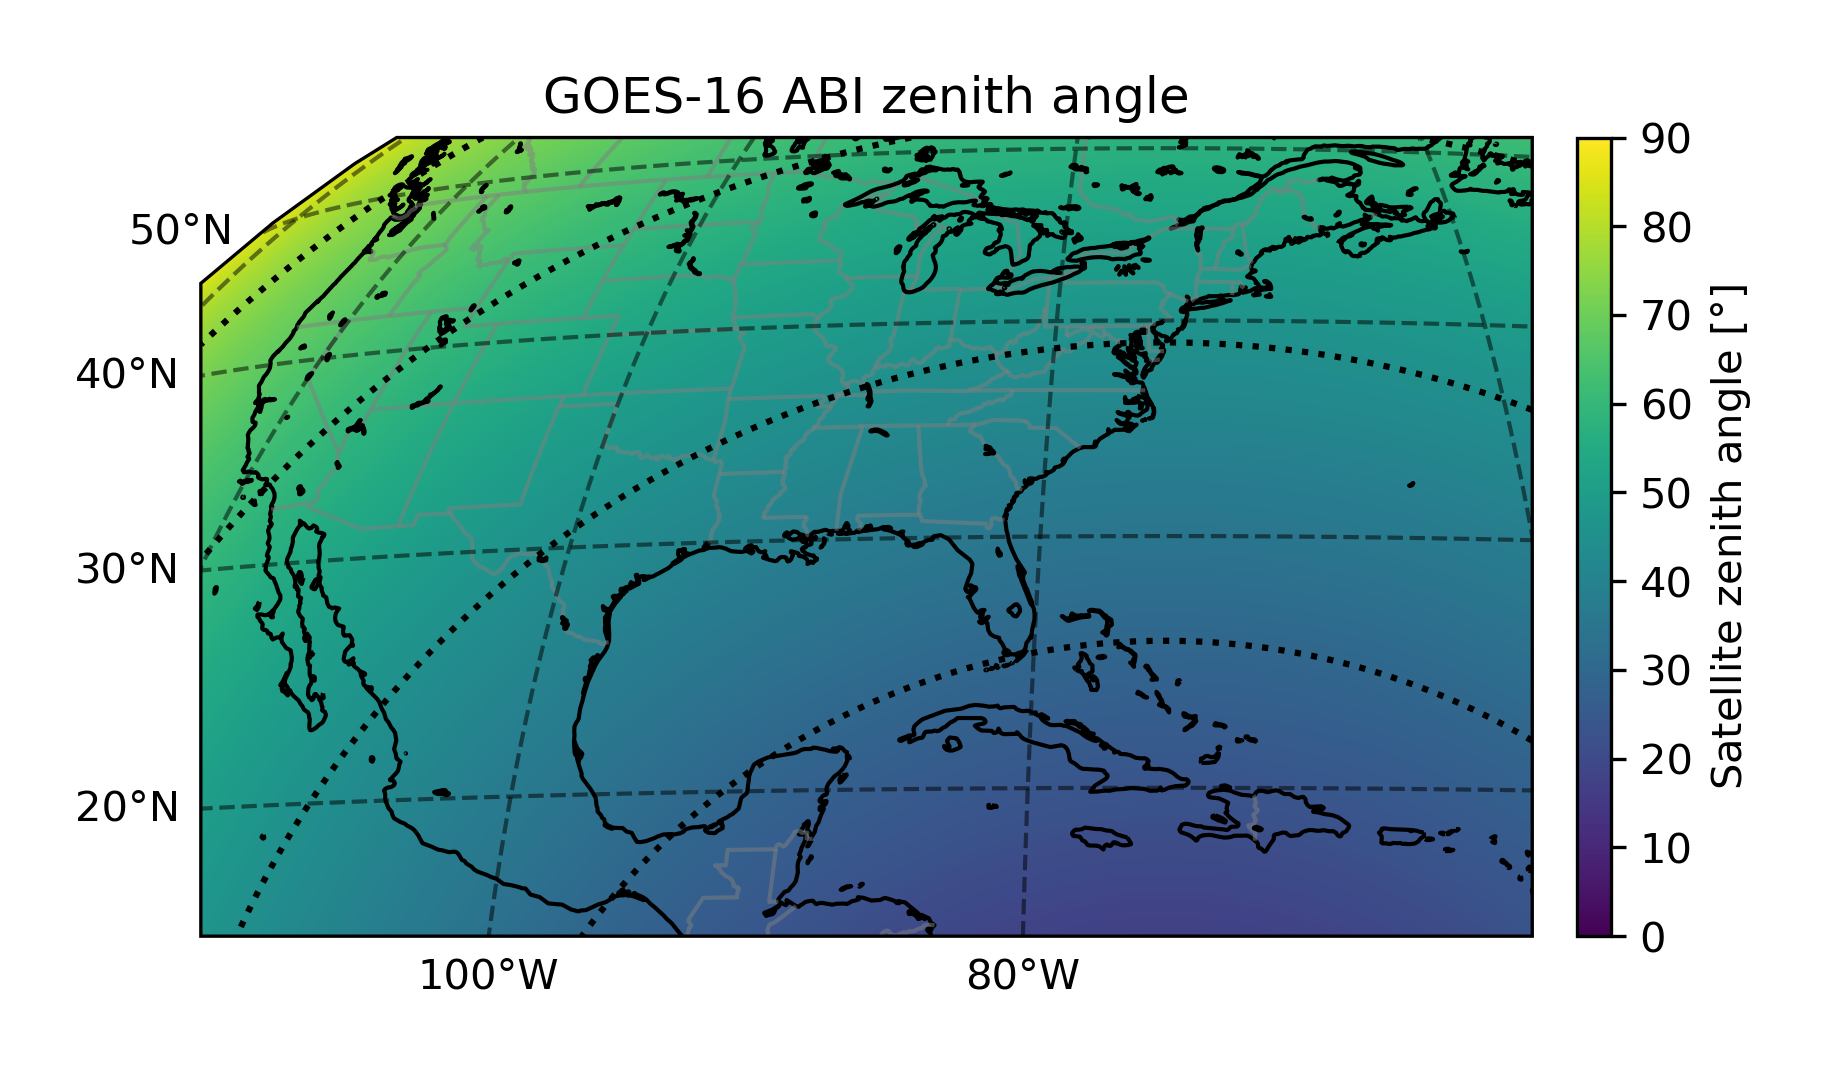
\includegraphics[width=\textwidth]{figures/chapter2_01.png}
    \caption[
    The sensor zenith angle of \acrshort{goes}-16 \acrshort{abi} observations across the \acrshort{conus} domain
    ]{
    The sensor zenith angle of \acrshort{goes}-16 \acrshort{abi} observations across the \acrshort{conus} domain. Dotted arcs are shown for each 15\,\textdegree interval of zenith angle.
    }
    \label{fig:abi_zenith_angles}
\end{figure}

To detect and track \acrshort{dcc}s across North America, \acrshort{abi} \acrshort{mcmip} data from the 6.2, 7.3, 10.4 and 12.4\,\unit{\mu m} channels observed in the \acrshort{conus} region is used, as described in section \ref{sec:abi_data}.
These observations span the full extent of the \acrshort{abi} \acrshort{conus} domain of 2,500~pixels E--W by 1,500~pixels N--S.
This domain covers a region of around 60--120\,\textdegree W in longitude and 15--50\,\textdegree N in latitude, covering an area of approximately 5,700 by 3,900\,\unit{km}.
Figure~\ref{fig:abi_zenith_angles} shows the satellite zenith angle of \acrshort{abi} observations across the \acrshort{conus} domain.
As the viewing angle increases the accurate detection and tracking of \acrshort{dcc}s becomes more difficult.
This is due to the confounding between vertical and horizontal motion, and also due to the area of each pixel increasing with the zenith angle.
The large sensor zenith angles in the North-West of the domain may introduce large errors in the detection and tracking algorithm, and so for the rest of this chapter only those \acrshort{dcc}s detected east of 110\,\textdegree W and south of 45\,\textdegree N are included in the analysis.

Five full years of data---from the start of 2018 to the end of 2022---are used to produce a dataset of detected \acrshort{dcc}s and their properties.
This period spans all complete years of operational data from \acrshort{goes}-16 \acrshort{abi}.
To improve to continuity of observations a gap-filling procedure is implemented.
If time gaps between observations of greater than 15 minutes are present, observations from the full-disc \acrshort{abi} scan are used to fill these gaps.
Full disc imagery is typically available every 10 or 15 minutes depending on the operating mode.
This gap filling is particularly important during the periods in which \acrshort{abi} uses its mode 4 scan pattern, in which no \acrshort{conus} domain scans are made, but the full disc is scanned every 5 minutes.
Using the full-disc observations allows us to maintain temporal sampling throughout these periods.


\section{Method} \label{sec:conus_method}

Detection and tracking of convective cores and anvil clouds are performed using the \textit{tobac-flow} method \citep{jones_semi-lagrangian_2023} described in section~\ref{sec:tracking_method}.
Initial detection of \acrshort{dcc}s is performed separately over 24-hour periods spanning from 12:00:00~\acrshort{utc} (approximately 6~am local time over North America) to the same time the next day.
This 24-hour period was dictated due to performance constraints, as the large domain combined with the high spatial and temporal resolution of \acrshort{abi} data results in a large memory requirement.
The start time corresponds with the minima of convective activity over land, and so was chosen to minimise the number of \acrshort{dcc}s missed at the start and end of the detection period.
Each period is extended by six \acrshort{abi} observations at each end to ensure at least one hour of overlap between successive days.

To track long-lived \acrshort{dcc}s that last beyond one day, a linking algorithm is used to combine \acrshort{dcc}s observed across multiple days.
The linking algorithm combines \acrshort{dcc}s detected at the same locations within the overlap period of two daily detection files.
Splitting and merging of objects is taken into account, so a single object which splits into two, or two objects which merge into one in the subsequent file are all considered a single, tracked object.
The linking algorithm is applied separately to each month of data for performance reasons.

%t
\begin{table}[b]
\centering
\begin{tabular}{ll}
\tophline
Core removed if:                                                    & Core invalid if: \\
\middlehline
Initial \acrshort{bt} -- final \acrshort{bt} \textless~8\,\unit{K}  & Intersects edge of domain \\
Lifetime \textless~15~minutes                                       & Intersects start of domain \\
Time gaps \textgreater~15~minutes                                   & Intersects end of domain \\
Maximum area \textgreater~10,000\,\unit{km\textsuperscript{2}}      & Adjacent to bad \acrshort{abi} data \\
Any NaN values in core properties                                   & \\
\bottomhline
\end{tabular}
\caption[
Validity criteria for detected cores
]{
Validity criteria for detected cores. Cores which flag any of the removal criteria are removed in their entirety from the dataset. Those which flag any of the invalid criteria are retained, but removed from subsequent analysis.}
\label{table:core_validity_criteria}
\end{table}

After linking, a processing step is applied to calculate the properties of detected cores and anvils at each step of their lifecycles.
Finally, core and anvil step properties are aggregated over each month of observation, and overall core and anvil properties are calculated.
During this final step quality flagging is performed to isolate detected features that fail one or more quality checks.
The quality criteria are split into two groups.
The first set of criteria---for core or anvil removal---removes features that cannot be verified as correctly tracked \acrshort{dcc}s due to bad data or a failure to meet the basic requirements for tracking described in chapter~\ref{chp:tracking_method}.
This may happen because there are large time gaps in the dataset, or missing data due to artifacts in the \acrshort{abi} observations.
Detected features which flag any of these criteria are removed from the aggregated dataset in their entirety.
This step in particular removes anvils which have no associated cores, or are not detected as initiating with a developing core.

The second set of criteria is used to identify detected cores or anvils that have not been observed over their entire extent or lifecycle.
Cores and anvils which flag any of these criteria are still included within the aggregated properties dataset, but are removed from the analysis \acrshort{dcc} properties throughout this chapter.
Quality criteria for cores are listed in table \ref{table:core_validity_criteria}, and those for anvils in table \ref{table:anvil_validity_criteria}.


%t
\begin{table}[tb]
\centering
\begin{tabular}{ll}
\tophline
Anvil removed if:                               & Anvil invalid if: \\
\middlehline
No associated cores                             & Intersects edge of domain \\
Lifetime \textless~15~minutes                   & Intersects start of domain \\             
Time gaps \textgreater~15~minutes               & Intersects end of domain \\
Maximum area \textless~maximum core area        & Adjacent to bad \acrshort{abi} data \\
Anvil detected before initial core              & Associated with invalid cores \\
Anvil dissipated before final core ends         & Maximum area reached before end \\
Any NaN values in anvil properties              & ~~of initial core \\
\bottomhline
\end{tabular}
\caption[
Validity criteria for detected anvils
]{
Validity criteria for detected anvil. Anvils which flag any of the removal criteria are removed in their entirety from the dataset. Those which flag any of the invalid criteria are retained, but removed from subsequent analysis. The majority of anvils removed are due to have no associated cores, or because the anvil was observed before any developing cores.}
\label{table:anvil_validity_criteria}
\end{table}


The complete processing pathway is outlined by the following steps:

\begin{enumerate}
    \item Detection of cores and anvils in \acrshort{abi} observations over each 24-hour period.
    \item Linking of overlapping objects detected in subsequent 24-hour periods over each month.
    \item Calculation of core and anvil step properties. 
    \item Quality criteria applied to core and anvils, properties aggregated over each month
\end{enumerate}

Two datasets are produced. The first consists of daily core and anvil spatial maps, with step properties, produced by processing step 3. 
The second, consisting of aggregated monthly core and anvil properties, is produced by step 4.

\begin{figure}[tp]
    \centering
    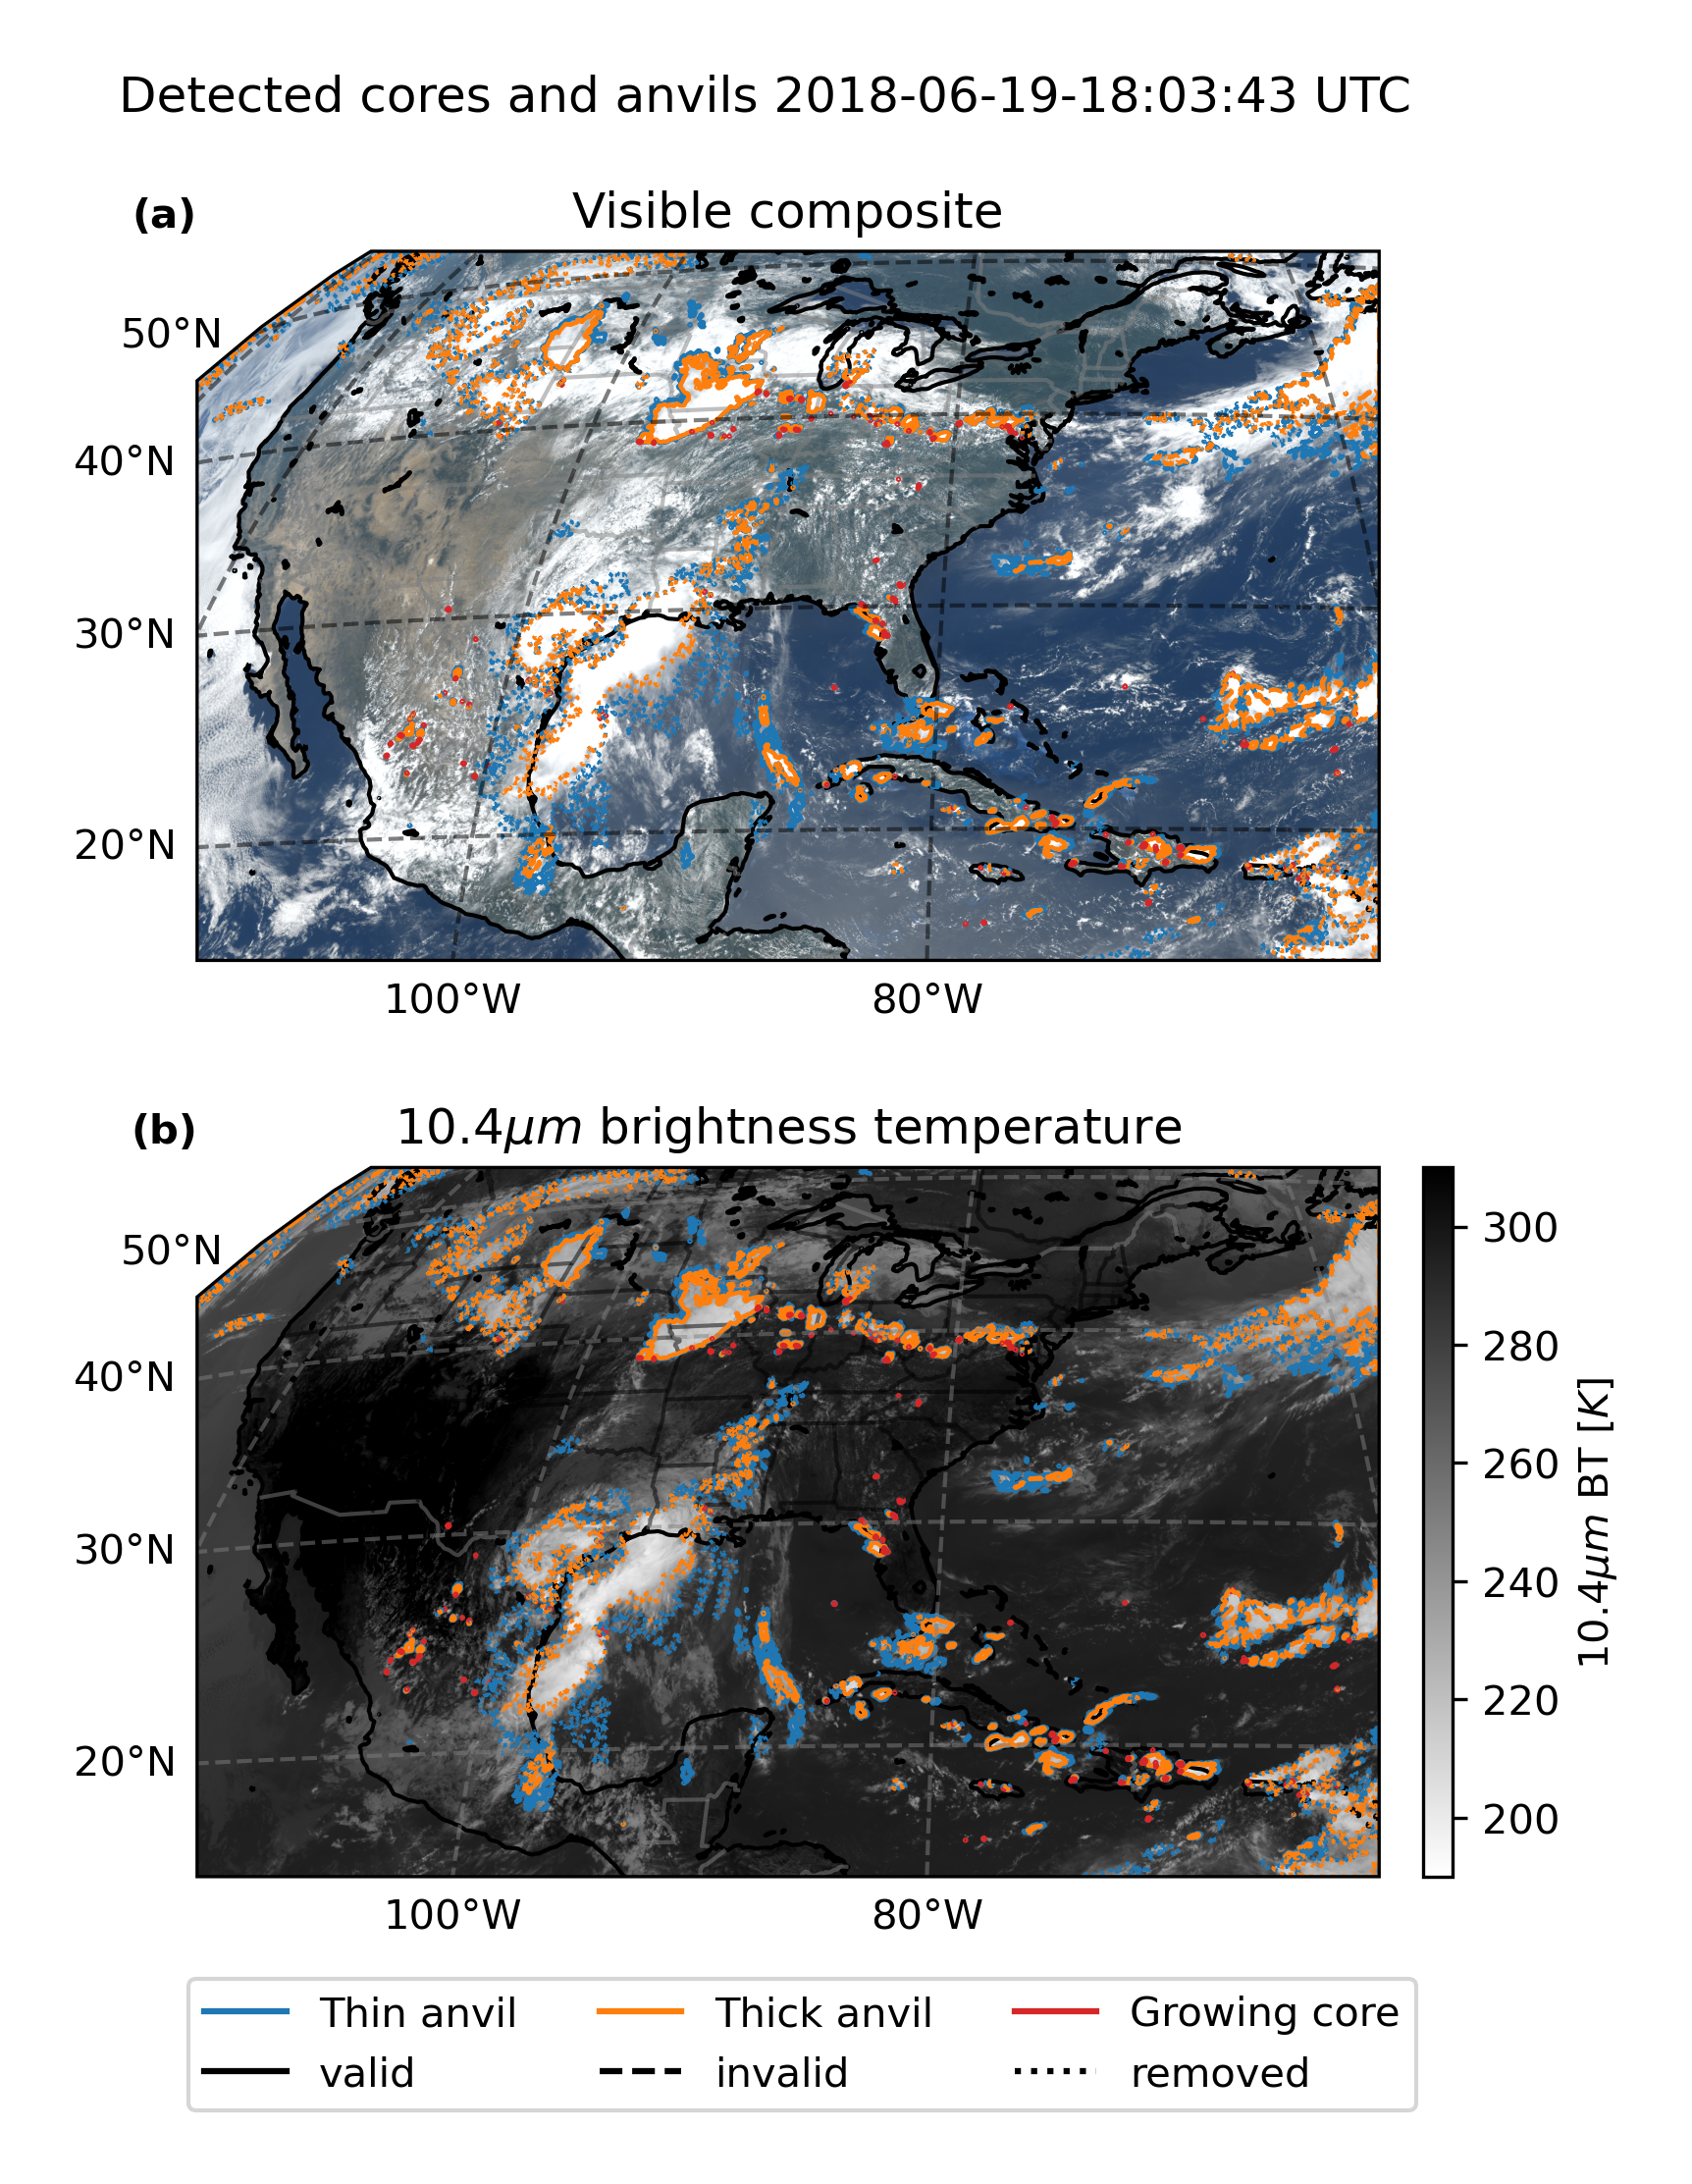
\includegraphics[width=\textwidth]{figures/chapter2_02.png}
    \caption[
    Detected cores and anvils from a snapshot of \acrshort{goes}-16 \acrshort{conus} domain observations
    ]{
    Detected cores and anvils from a snapshot of \acrshort{goes}-16 \acrshort{conus} domain observations. Cores and anvils removed from the aggregated dataset are shown with dotted outlines. Those which are flagged as invalid are shown with dashed outlines. Detected features are shown against (a) visible composite imagery and (b) 10.4\,\unit{\mu m} \acrshort{bt}
    }
    \label{fig:conus_detected_dccs}
\end{figure}

Figure~\ref{fig:conus_detected_dccs} shows an example of detected cores and anvils over the \acrshort{conus} region, against backgrounds of composite visible imagery (fig.~\ref{fig:conus_detected_dccs}\,a) and 10.4\,\unit{\mu m} \acrshort{bt} (fig.~\ref{fig:conus_detected_dccs}\,b).
Cores and anvils which are removed from the aggregated dataset are outlined with dotted lines, and those which are considered invalid are shown with dashed outlines.
The large, organised convective system centred at 95\,\textdegree W, 27\,\textdegree N has been removed as it is intersected by a scan-line artifact later in its lifetime.
The \acrshort{dcc}s observed along the eastern edge of the domain have been marked invalid as, while they are considered true detections of \acrshort{dcc}s, they intersect the edge of the domain.

Over the five-year observing period a total of 3,877,130 cores are detected, of which 3,615,533 are considered valid, and 1,643,030 are linked with an anvil cloud. 
A total of 648,345 anvils are detected, of which 391,050 are valid, and these valid anvils contain 792,522 cores.
The disparity in the number of valid cores and the number of cores contained with valid anvils is due to additional filtering applied to the anvils.
As the larger and longer-lived anvils are more likely to intersect the edges of the domain, they are more likely to be marked invalid than the cores.
In these cases, the cores themselves are valid for analysis, but the anvil itself is excluded from analysis as its entire extent and lifetime are not captured.
The exclusion of anvils that intersect the edges of the domain introduces a bias towards removing larger, long-lived systems near the edge of the domain, which should be considered when assessing the properties of the observed \acrshort{dcc}s.


\section{Results}


\subsection{Distributions and properties of developing convective cores} \label{sec:core_properties}

%f
\begin{figure}[!tp]
    \centering
    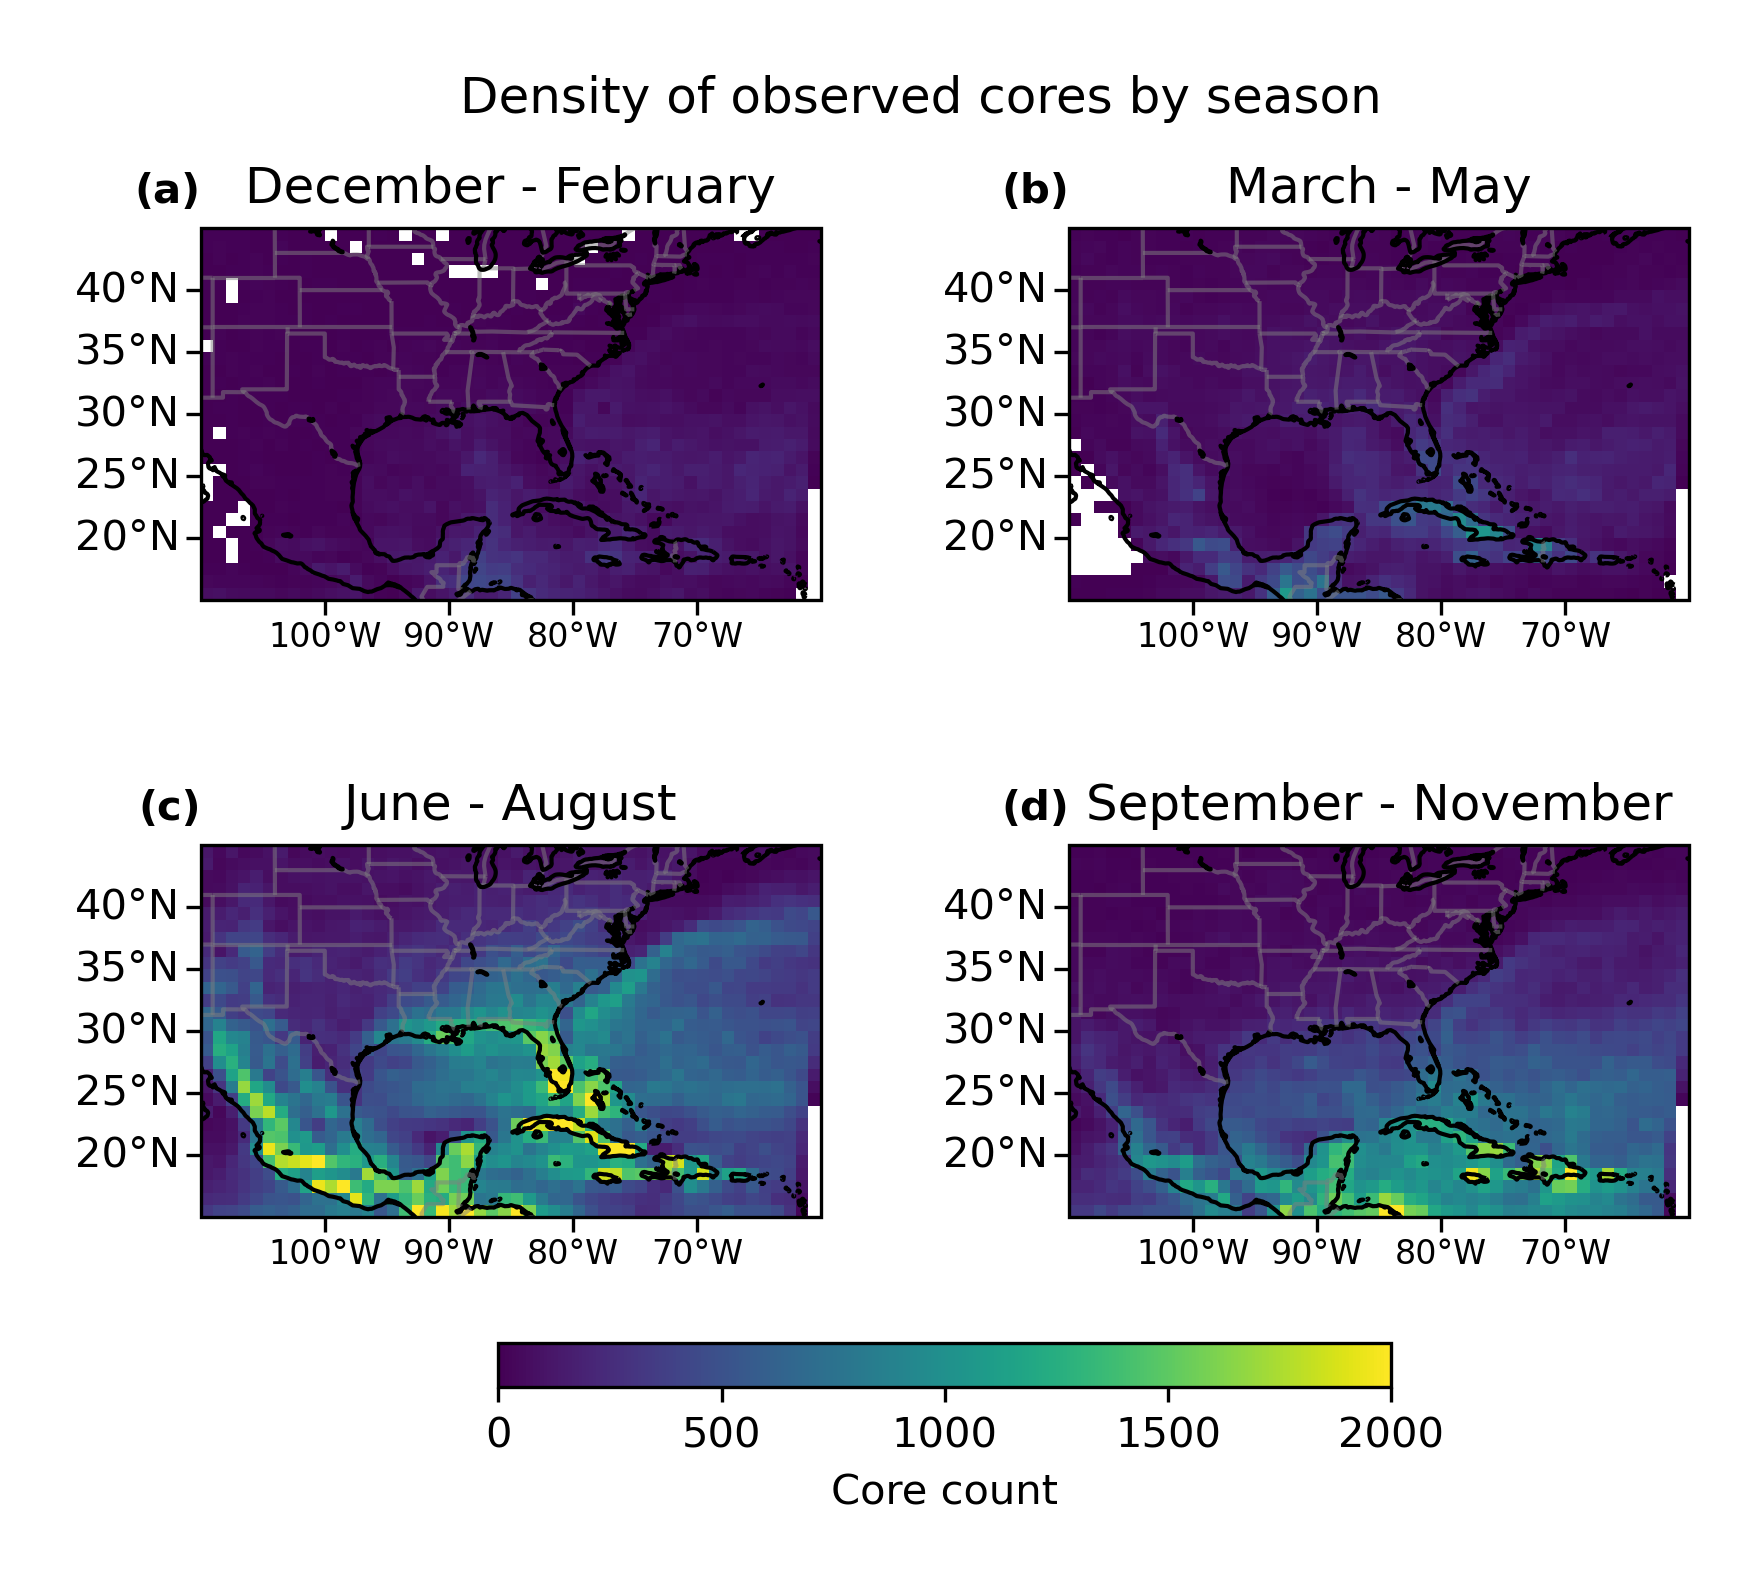
\includegraphics[width=\textwidth]{figures/chapter2_03.png}
    \caption[
    The spatial distribution of observed cores by season
    ]{
    The spatial distribution of observed cores, broken down by season and accumulated into 1\texttimes1\textdegree\ grid boxes of latitude and longitude. The density of observed cores is greatest during summer (c) and smallest during winter (a).
    }
    \label{fig:core_density_by_season}
\end{figure}

To begin, the distribution of detected \acrshort{dcc} cores throughout the dataset is investigated.
Figure~\ref{fig:core_density_by_season} shows the distribution of observed cores over North America separated by season.
Large variations in the spatial distribution of cores can be observed across the different seasons.
Overall, in winter and spring (fig.~\ref{fig:core_density_by_season}\,a,b) there are lower rates of observed \acrshort{dcc}s than in the summer and autumn (fig.~\ref{fig:core_density_by_season}\,c,d).

%f
\begin{figure}[!tp]
    \centering
    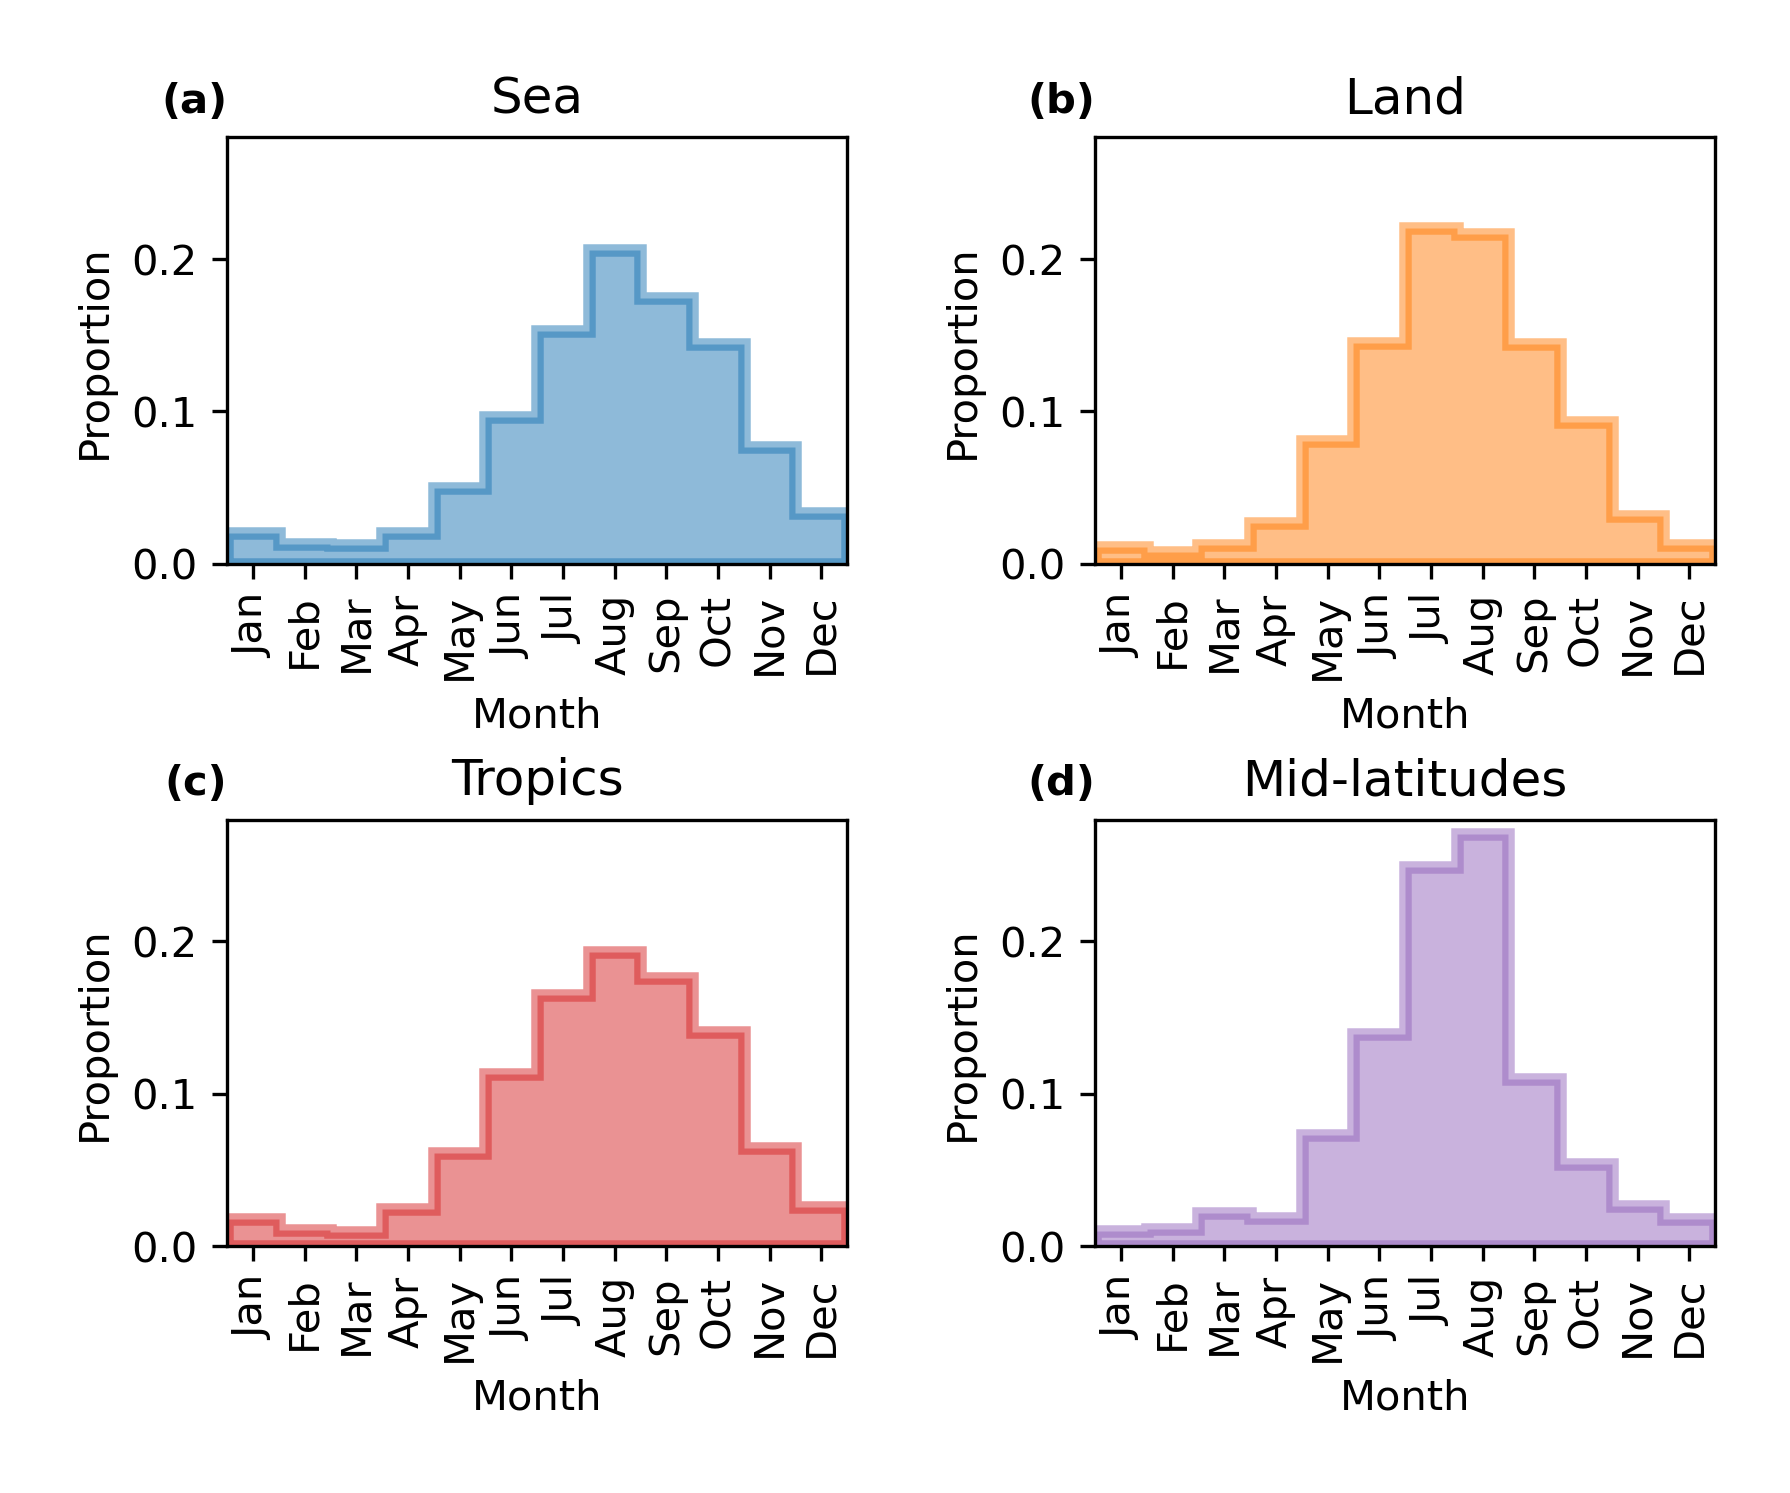
\includegraphics[width=\textwidth]{figures/chapter2_04.png}
    \caption[
    Monthly distributions of the proportion of cores detected each month over land, sea, tropics and mid-latitudes
    ]{
    Monthly distributions of the proportion of cores detected each month over (a) sea, (b) land, (c) tropics (\textless 30\,\textdegree N) and (d) mid-latitudes (\textgreater 30\,\textdegree N).
    }
    \label{fig:core_annual_land_sea}
\end{figure}

In winter (fig.~\ref{fig:core_density_by_season}\,a) the majority of convection observed occurs over the ocean, particularly in the areas of the Gulf of Mexico and West Atlantic associated with warm currents.
In spring (fig.~\ref{fig:core_density_by_season}\,b), a similar pattern shows over the ocean, and there is also an increase in convection detected over land in the Caribbean, Mexico and the central and southern \acrshort{usa}.
In summer (fig.~\ref{fig:core_density_by_season}\,c) there is a large increase in convection over land and ocean, with the highest rates of convection of any season.
There are, in particular, high rates of convection over Mexico, the Caribbean, the southern \acrshort{usa} (Florida in particular) and adjacent ocean regions.
In autumn (fig.~\ref{fig:core_density_by_season}\,d) there is a large reduction in the number of convective cores detected over land regions.
The number of detections over the ocean remains high, however, indicating a possible lag in the seasonal cycle of convection over oceans compared to that over land.

Figure~\ref{fig:core_annual_land_sea} shows the proportion of cores detected in each month over the annual cycle for land and sea regions.
Both land and sea regions show a peak of convective activity in the summer and a low in the winter months.
However, as suggested by fig.~\ref{fig:core_density_by_season}, there is a time lag of about 1 month between the annual cycle of convection over land and that over the ocean, likely due to the time lag in ocean heating.
Comparing the tropics and mid-latitudes, the monthly distribution of convection is much more sharply focused on July--August in the mid-latitudes compared to the broader distribution seen in the tropics.


%f
\begin{figure}[tp]
    \centering
    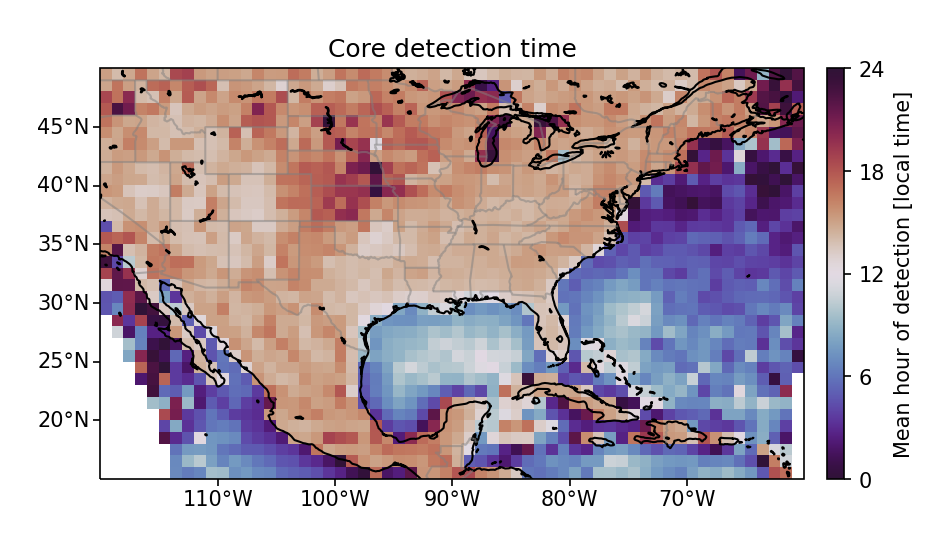
\includegraphics[width=\textwidth]{figures/chapter2_05.png}
    \caption[
    The average speed and direction of propagation of cores
    ]{
    The average speed and direction of propagation of cores observed within each 1\texttimes1\textdegree\ grid box. The colouring shows the average speed of propagation, and the red arrows show the average direction for each 2\texttimes2\textdegree\ grid box}
    \label{fig:core_propagation_map}
\end{figure}

Figure~\ref{fig:core_propagation_map} shows the average speed of propagation for cores observed in each 1-degree grid box, with the average direction of propagation shown by arrows for each 2-degree grid box.
There is a clear change in the direction of propagation from an easterly motion in the tropics (below 25\,\textdegree N) to a south-westerly motion in the mid-latitudes.

%f
\begin{figure}[tp]
    \centering
    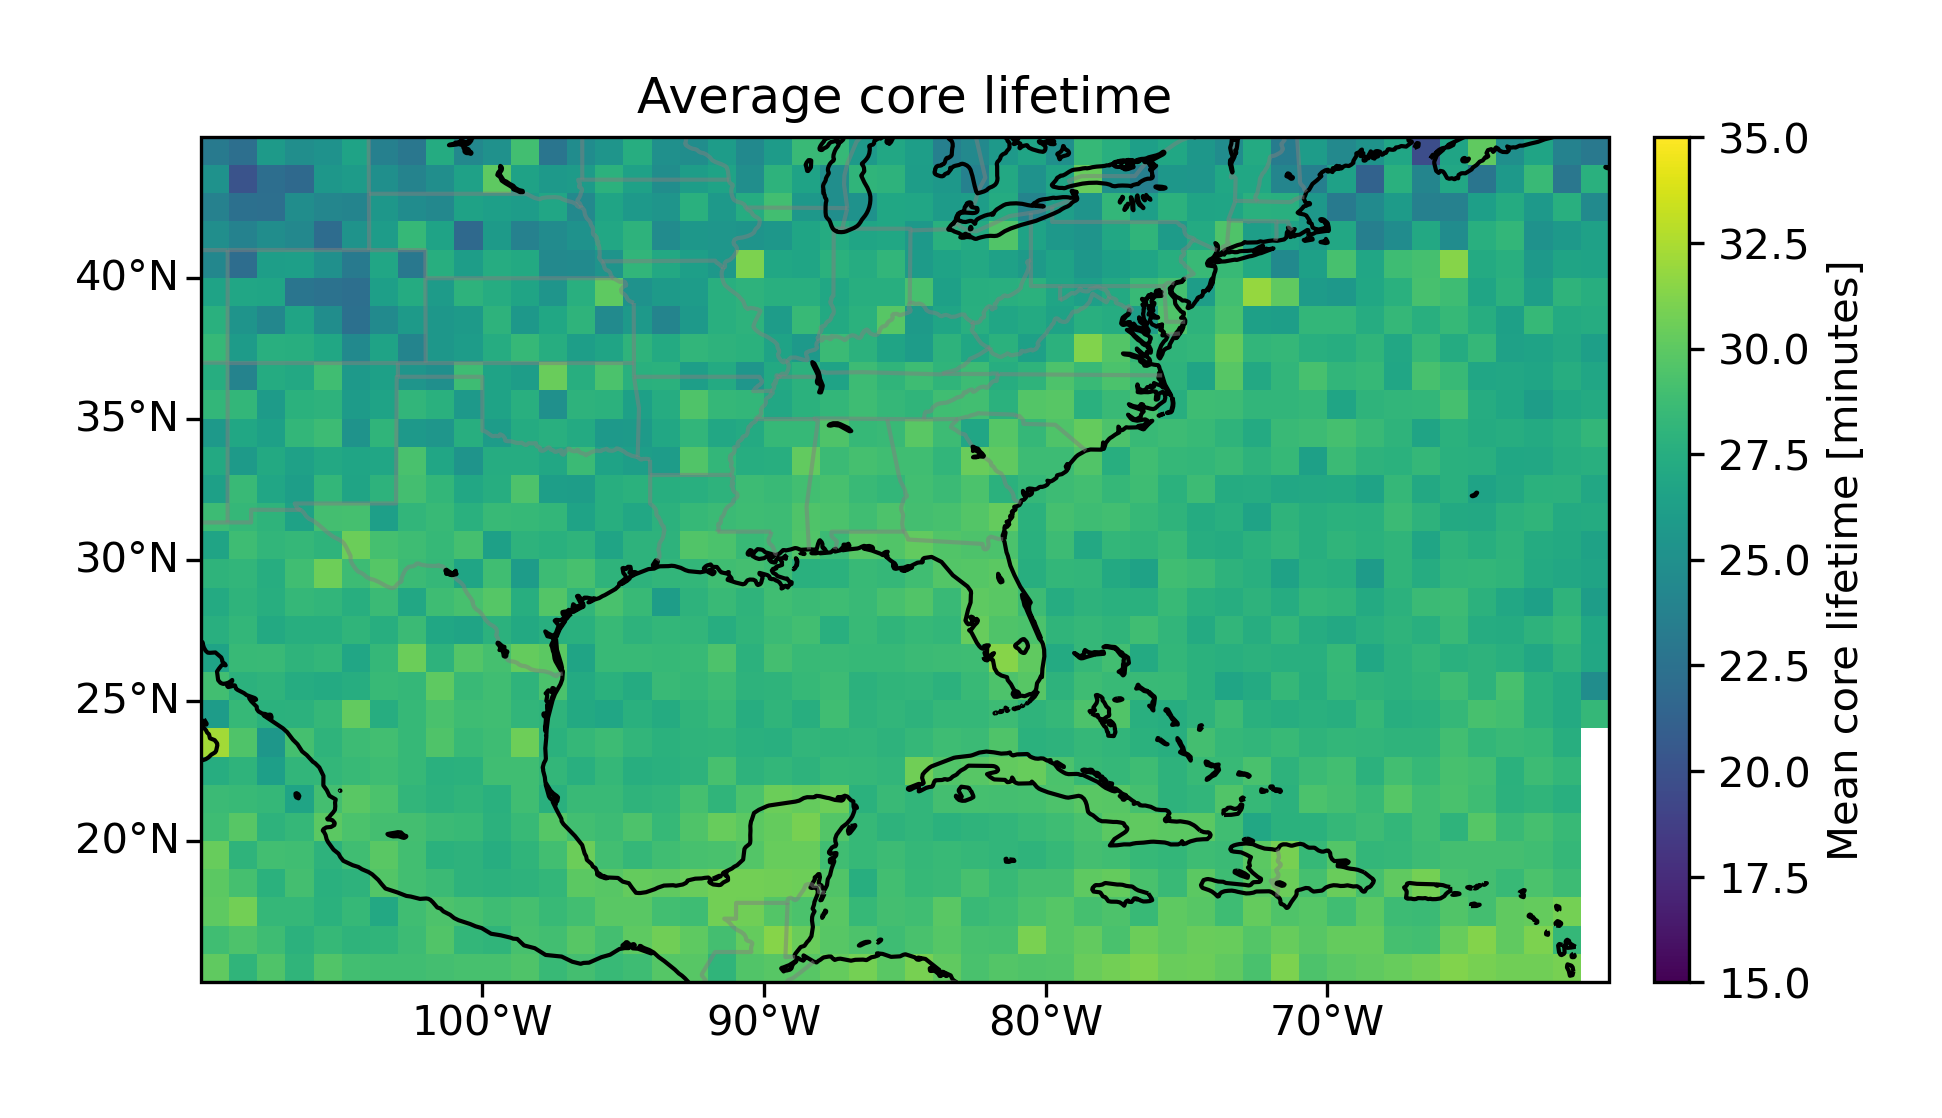
\includegraphics[width=\textwidth]{figures/chapter2_06.png}
    \caption[
    A map showing the mean lifetime in minutes of cores within each 1\texttimes1
    \textdegree\ grid box
    ]{
    A map showing the mean lifetime in minutes of cores within each 1\texttimes1
    \textdegree\ grid box.
    }
    \label{fig:core_lifetime_map}
\end{figure}

Figure \ref{fig:core_lifetime_map} displays the mean lifetime of observed cores over each 1-degree box of latitude and longitude.
The lifetime is defined as the period of time over which each core is detected, which represents the time in which to core is developing vertically.
Convection will continue in the core after this point, but the motion of the cloud top will instead be a horizontal divergence of the anvil.
The average lifetimes appear mostly uniform across the domain, with a small reduction with increasing latitude.
This reduction in the lifetime of the developing core at higher latitudes is likely due to the lower tropopause height restricting the vertical development of the cores.
Similarly, there is a slight reduction in average lifetime over the more mountainous, inland regions of Mexico compared to the adjacent coastal regions.
This again may be linked to the reduction in the depth of the convective cores, although in this case due to an increased surface height rather than a lower tropopause.


%f
\begin{figure}[tp]
    \centering
    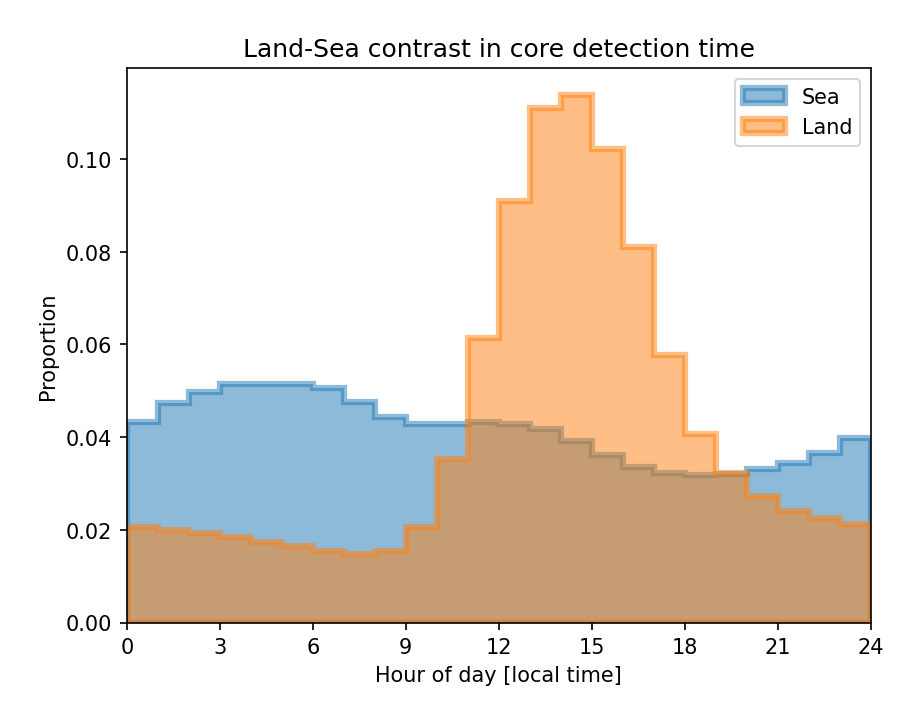
\includegraphics[width=\textwidth]{figures/chapter2_07.png}
    \caption[
    A map of the average maximum core cooling rate for each 1\texttimes1
    \textdegree\ grid box
    ]{
    A map of the  average maximum core cooling rate for each 1\texttimes1
    \textdegree\ grid box.
    }
    \label{fig:core_cooling_rate_map}
\end{figure}

Figure~\ref{fig:core_cooling_rate_map} shows the average cooling rate of observed cores.
The contrasts here are more pronounced than those shown in fig.~\ref{fig:core_lifetime_map}.
There is a reduction in the average cooling rate with latitude, likely due to the reduction in solar heating and hence lower \acrshort{cape}.
Orography also has a factor, with lower cooling rates observed over the mountains of Mexico and the North American Rockies.
The largest average core cooling rates are observed in coastal regions, indicating potential land--sea interactions.

%f
\begin{figure}[tp]
    \centering
    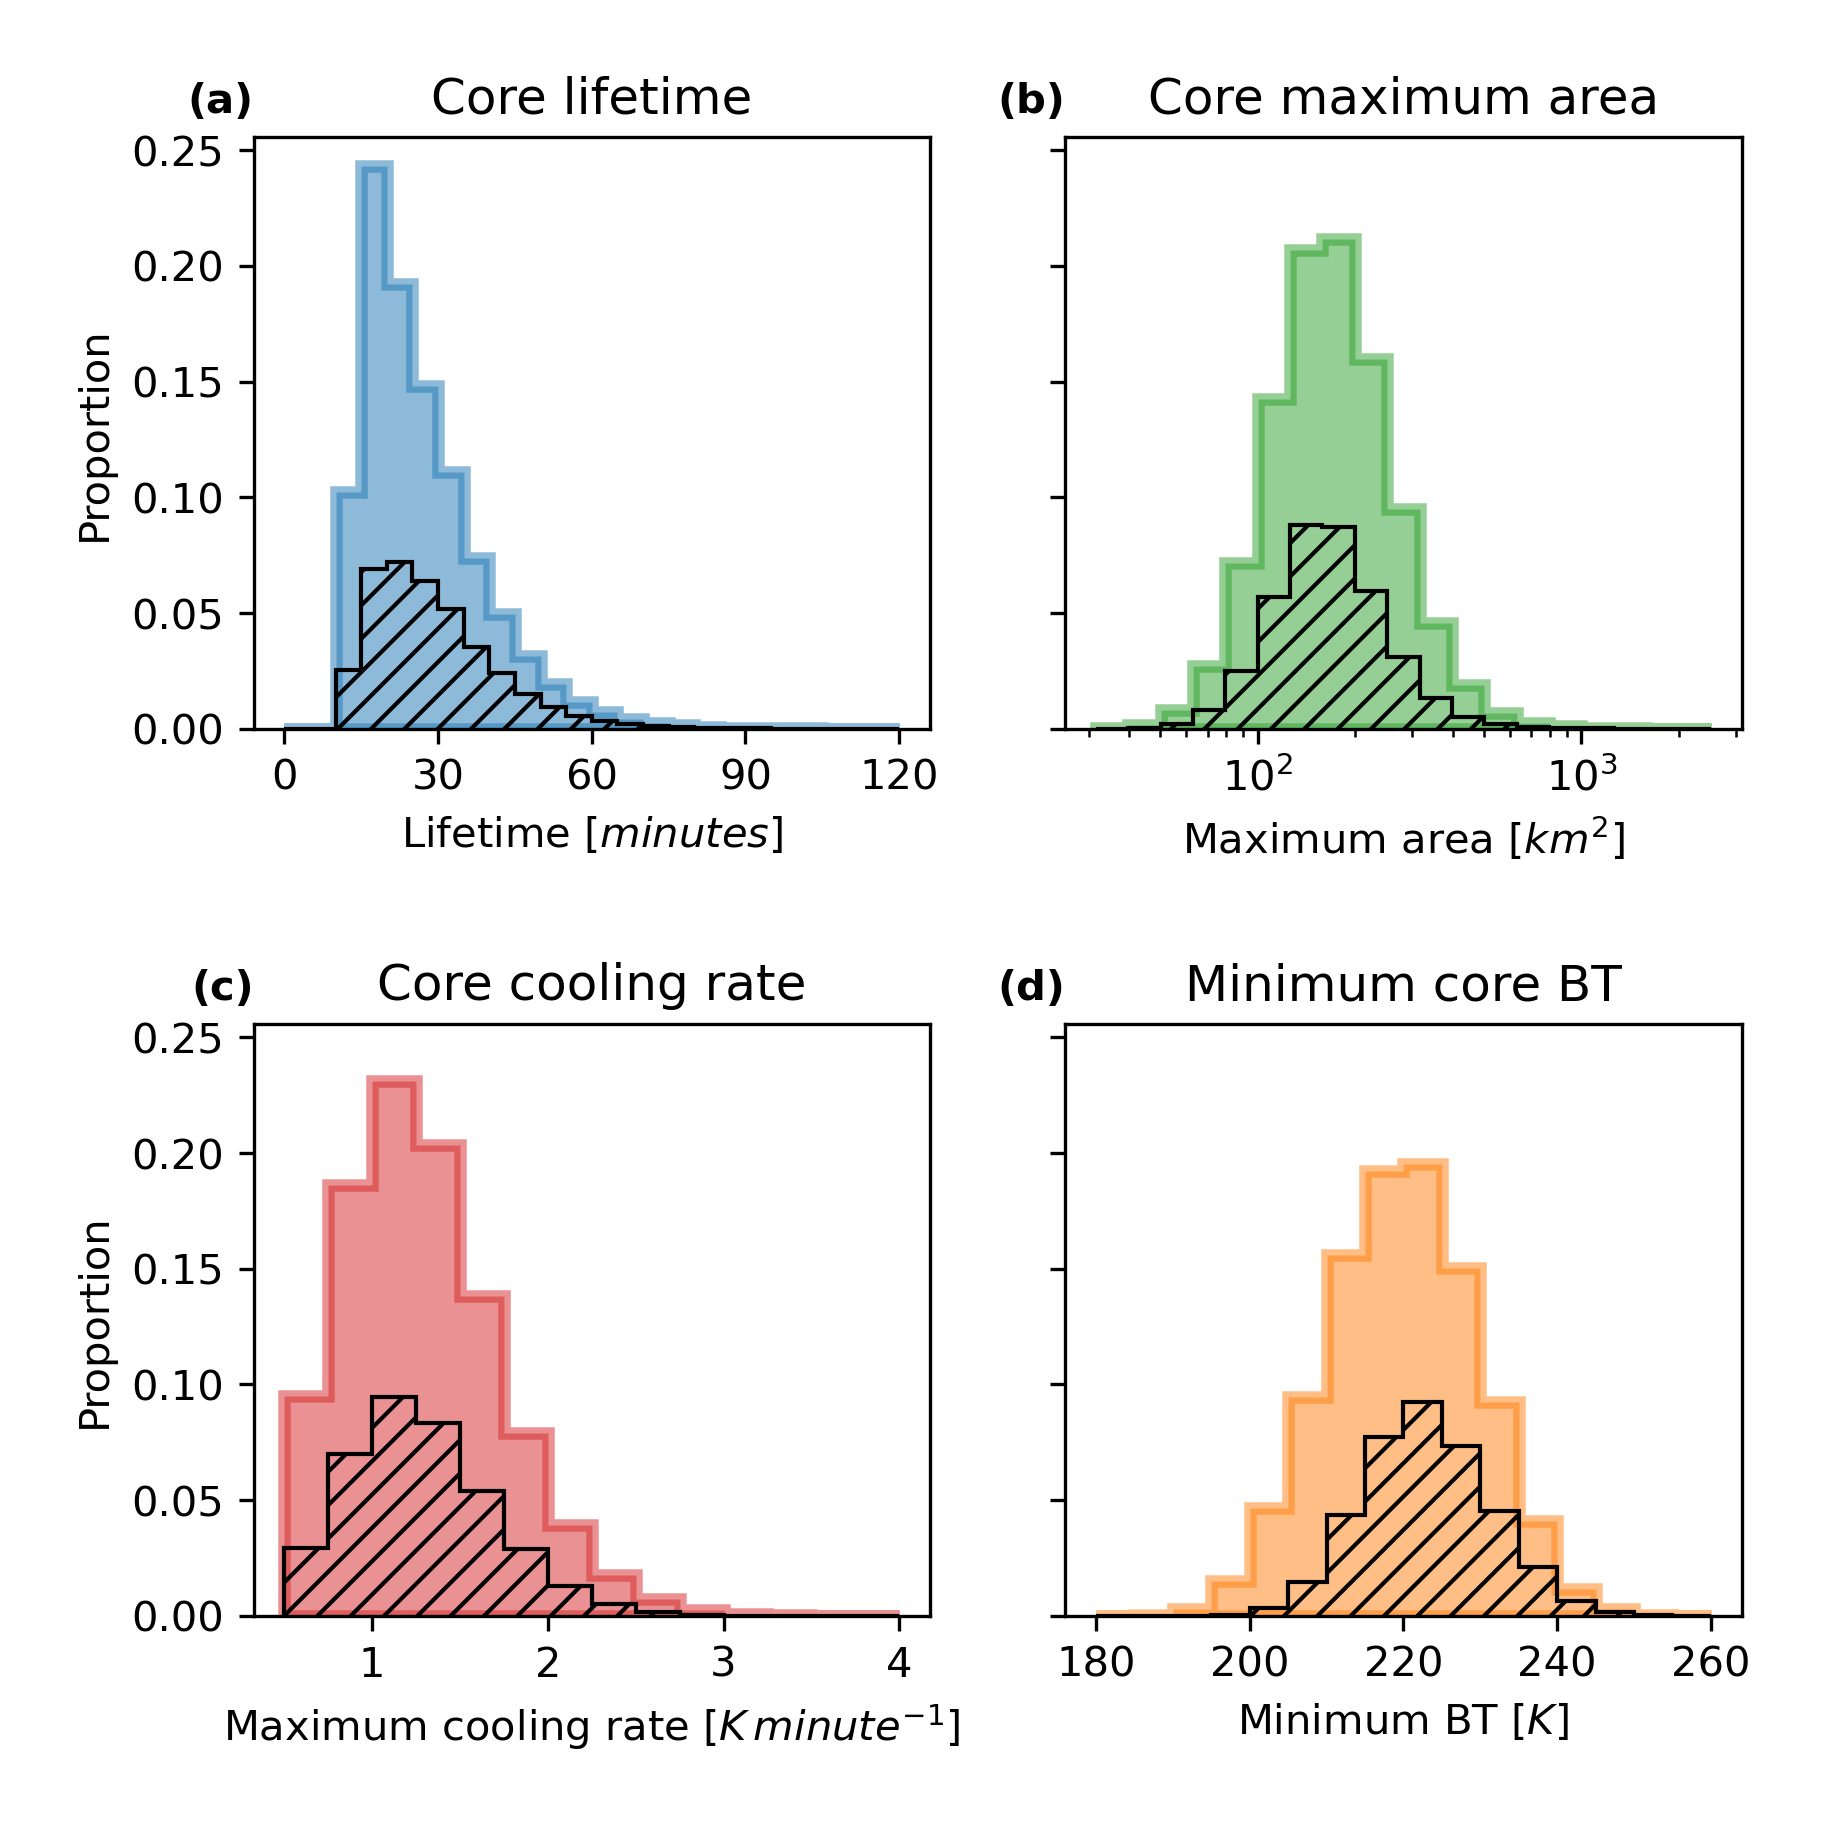
\includegraphics[width=\textwidth]{figures/chapter2_08.png}
    \caption[
    Histograms showing the distributions of observed core lifetimes, maximum areas, cooling rates and \acrshort{bt}
    ]{
    Histograms showing the distributions of observed (a) core lifetime, (b) maximum area, (c) maximum cooling rate, (d) and minimum \acrshort{bt}. The hatched areas show the proportion of each distribution consisting of the initial detected cores within each tracked \acrshort{dcc}.
    }
    \label{fig:core_properties}
\end{figure}

Figure~\ref{fig:core_properties} shows the distributions of lifetime (fig.~\ref{fig:core_properties}\,a), maximum area (fig.~\ref{fig:core_properties}\,b), cooling rate (fig.~\ref{fig:core_properties}\,c), and minimum \acrshort{bt} (fig.~\ref{fig:core_properties}\,d).
There is a peak in the observed lifetime of cores between 15 and 20 minutes, with a large tail extending beyond 60 minutes in some cases.
Note that due to the requirement of a minimum of three consecutive observations, cores lasting less than 10 minutes will not be detected, truncating the distribution.
In fig.~\ref{fig:core_properties}\,b the maximum core area peaks around 150--200\,\unit{km\textsuperscript{2}}, representing cores approximately 12--14 km in diameter.
Figure~\ref{fig:core_properties}\,c shows that the core cooling rate peaks at values of 1--1.25\,\unit{K minute\textsuperscript{-1}}, representing vertical cloud top velocities of approximately 2.5--3\,\unit{ms\textsuperscript{-1}}.
The distribution is slightly truncated by the requirement for detected cores to have a cooling rate of at least 0.5\,\unit{K minute\textsuperscript{-1}}.

The minimum core \acrshort{bt} distribution (fig.~\ref{fig:core_properties}\,d) peaks at around 220\,\unit{K}, supporting the theory that the radiative tropopause sets the height of the convectively active layer of the atmosphere.
Many cores reach temperatures warmer than 220\,K, indicating either a lower \acrshort{lnb} or dilution of the convective updraft leading to reduced buoyancy.
In addition, a large number of cores reach \acrshort{bt} colder than 220\,K, which, for the coldest cases, likely indicates the occurrence of overshooting tops.

The hatched areas in fig.~\ref{fig:core_properties} show the proportion of each distribution consisting of the initial cores of tracked \acrshort{dcc}s.
As their development will not be masked by an overlaying anvil cloud, these cores are expected to provide the most complete measurements of developing core properties.
For the lifetime, maximum area and cooling rate these show close similarities to the shape of the distribution for all cores, indicating that masking due to anvils does not significantly affect the ability to observe the core properties.
For the minimum core \acrshort{bt}, the initial cores tend to have warmer \acrshort{bt} than later cores, indicating an increased presence of cold cores and overshooting tops in organised convection.

%f
\begin{figure}[tp]
    \centering
    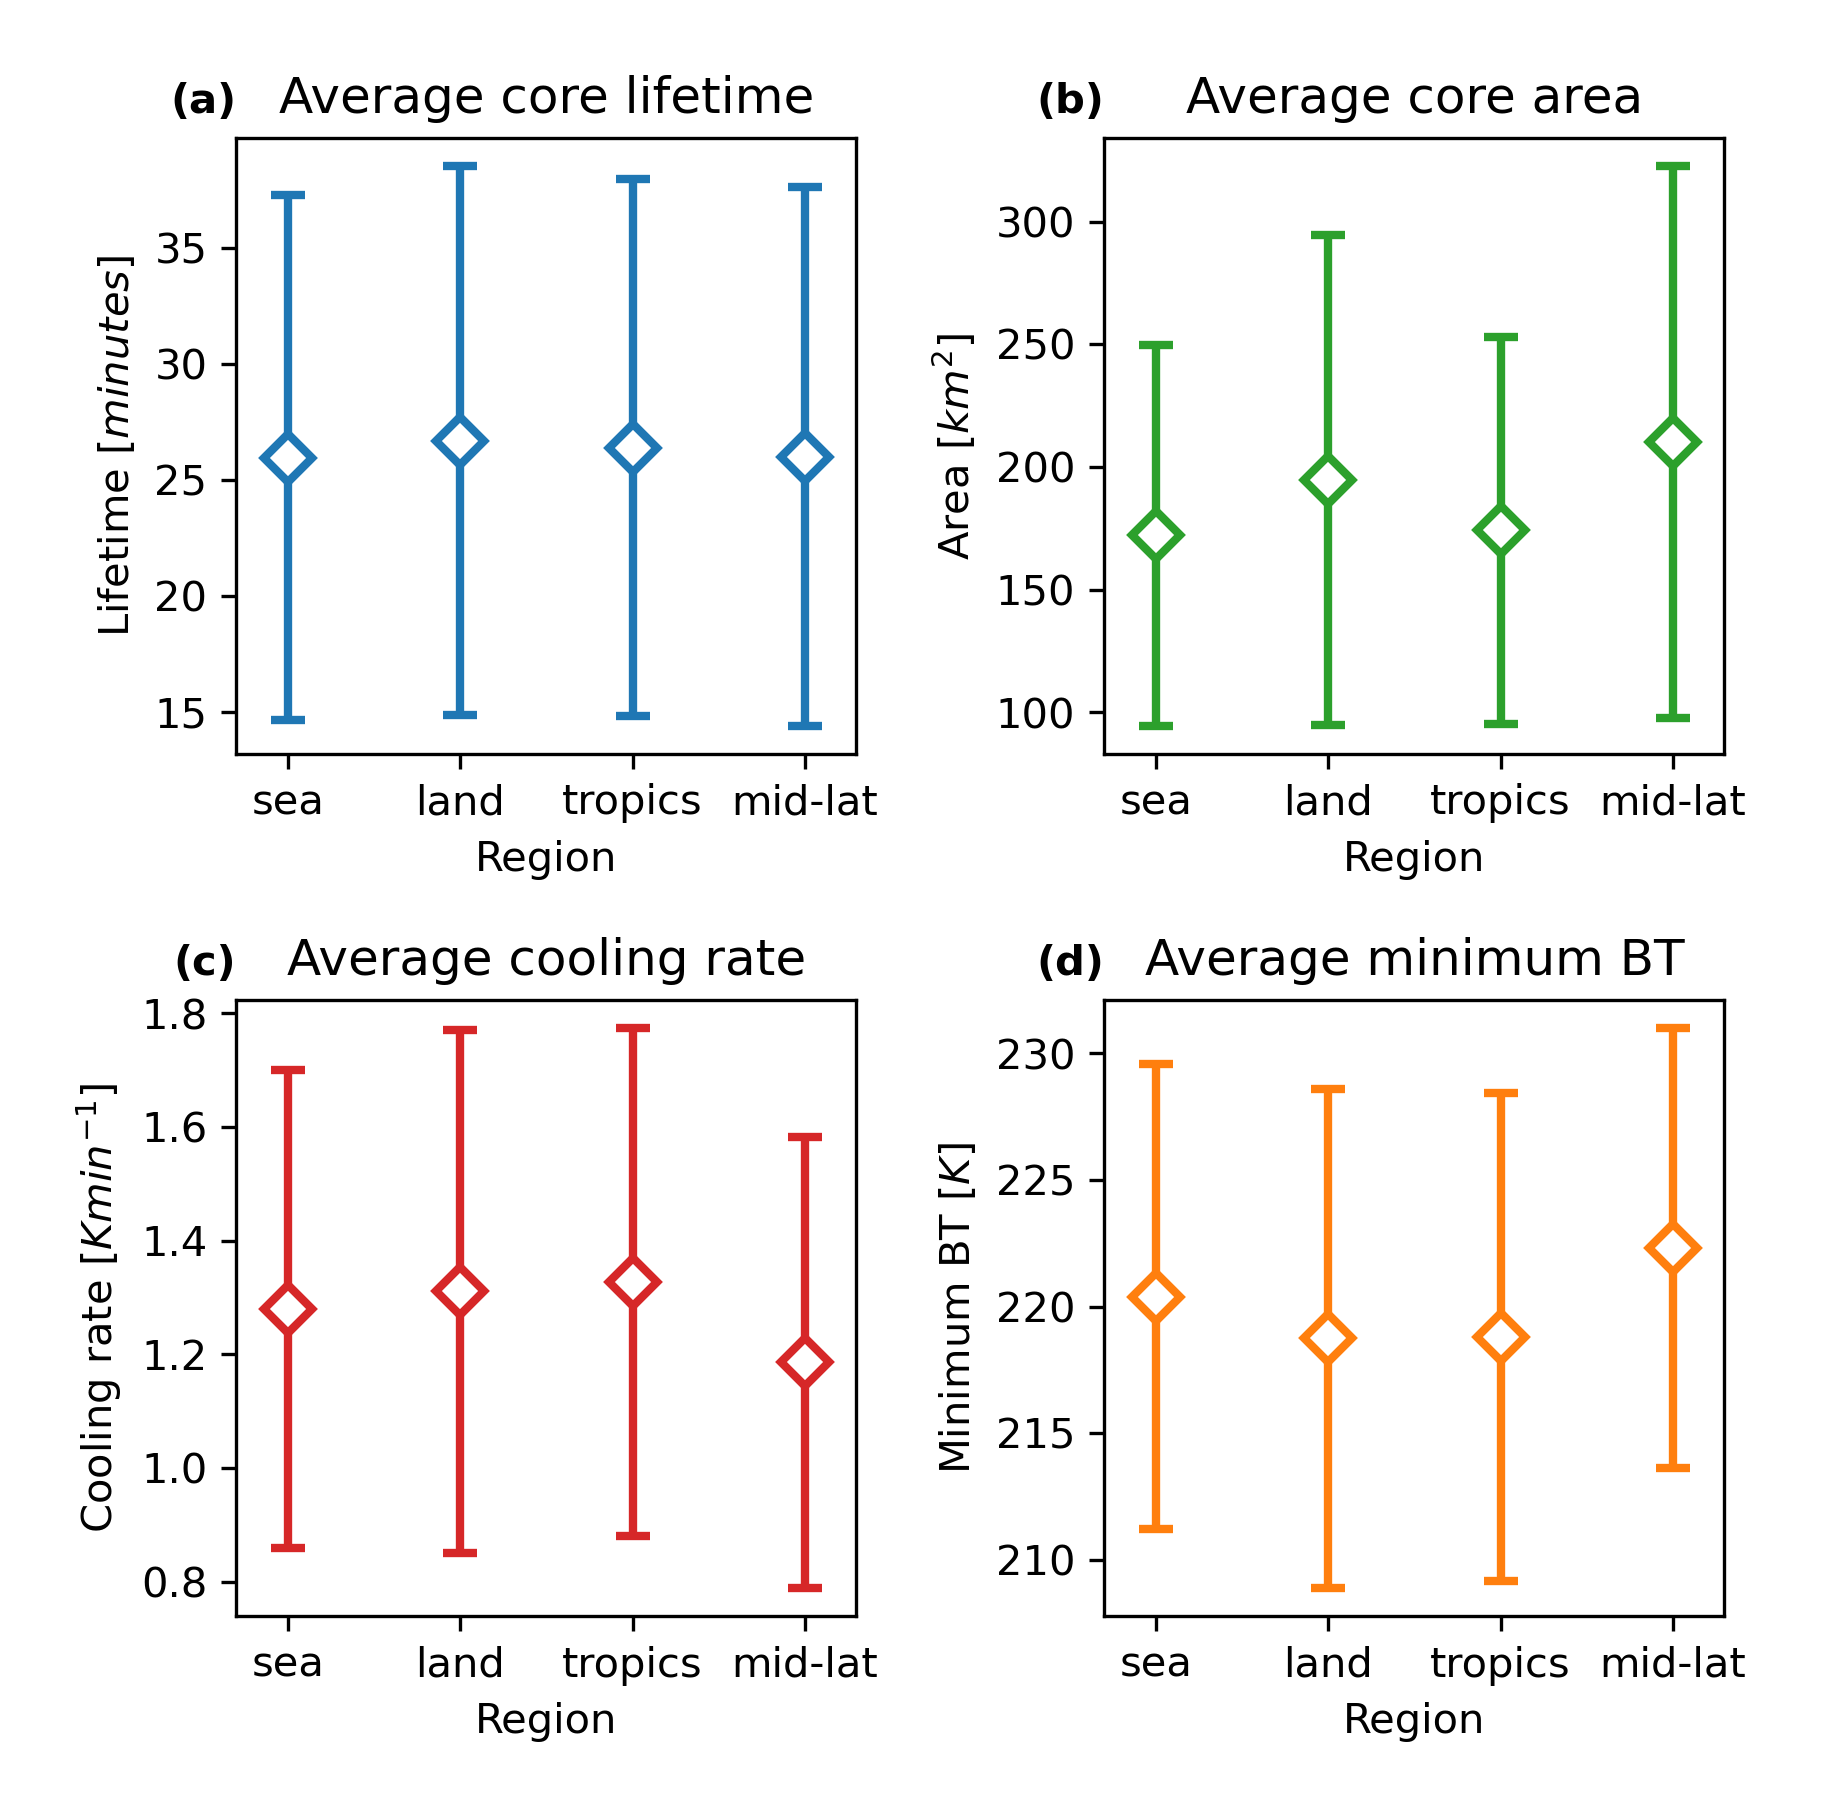
\includegraphics[width=0.75\textwidth]{figures/chapter2_09.png}
    \caption[
    The mean observed lifetimes, maximum areas, cooling rates and \acrshort{bt} for cores detected over land, sea, tropics and mid-latitudes
    ]{
    The mean observed (a) lifetime, (b) maximum area, (c) maximum cooling rate, (d) and minimum \acrshort{bt} for cores detected over land, sea, tropics and mid-latitudes. Error bars are not shown as the standard error of the mean is too small to be visible.
    }
    \label{fig:core_region_mean_properties}
\end{figure}

Figure~\ref{fig:core_region_mean_properties} shows how the mean core lifetime, maximum area, cooling rate and \acrshort{bt} vary between different regions.
There is little difference in the mean core lifetime between regions, echoing the results seen in fig.~\ref{fig:core_lifetime_map}.
Maximum core area is larger over land than sea, and larger in the mid-latitudes than in the tropics.
There is little difference in the cooling rate between sea and land, but on average cores in the tropics cool $\sim$0.2\,\unit{K minute\textsuperscript{-1}} faster than those in the mid-latitudes.
There is a small difference in the minimum \acrshort{bt} of cores observed over land and ocean, with the former $\sim$1.5\,\unit{K} colder than the latter.
A more noticeable difference is seen with latitude, with cores in the tropics having, on average, minimum \acrshort{bt} $\sim$3\,\unit{K} colder than those in the mid-latitudes.

Overall, fig.~\ref{fig:core_region_mean_properties} show differences in core intensity between land and ocean, and between the tropics and mid-latitudes, with these differences most prominent in the minimum \acrshort{bt}.
Due to the large number of tracked cores, the standard error of the mean for each point is very small, and so from a simple perspective these differences appear significant.
However, the impact of systematic bias on these properties must also be considered, in particular the impact of the sensor zenith angle as discussed in sections~\ref{sec:abi_channels} and \ref{sec:lifecycle_data}, which may impact the detection accuracy and measured properties of tracked \acrshort{dcc}s.
As more of the ocean observations are in the tropics, and more of the land \acrshort{dcc}s observed in the mid-latitudes, covariance should be expected between the average properties of \acrshort{dcc}s in these regions.
In fig.~\ref{fig:core_region_mean_properties}\,b larger average areas are seen for both land over ocean and mid-latitudes over the tropics, indicating that the differences may be the result of the expected systematic bias in area caused by sensor zenith angle.
However, for the other three properties, while convective cores over land have longer lifetimes, higher cooling rates and colder minimum \acrshort{bt} than those over the ocean, cores in the tropics also have the same indicators of more intense convection when compared to the mid-latitudes.
This opposes the expected covariance between these regions, and indicates that the differences seen are likely to be real and significant, and that the systematic error is smaller than the differences seen between land and ocean and between tropics and mid-latitudes.
These differences may result from changes in different convective processes as the difference in cooling rate between tropics and mid-latitudes is as large when comparing sea and land.

%f
\begin{figure}[tp]
    \centering
    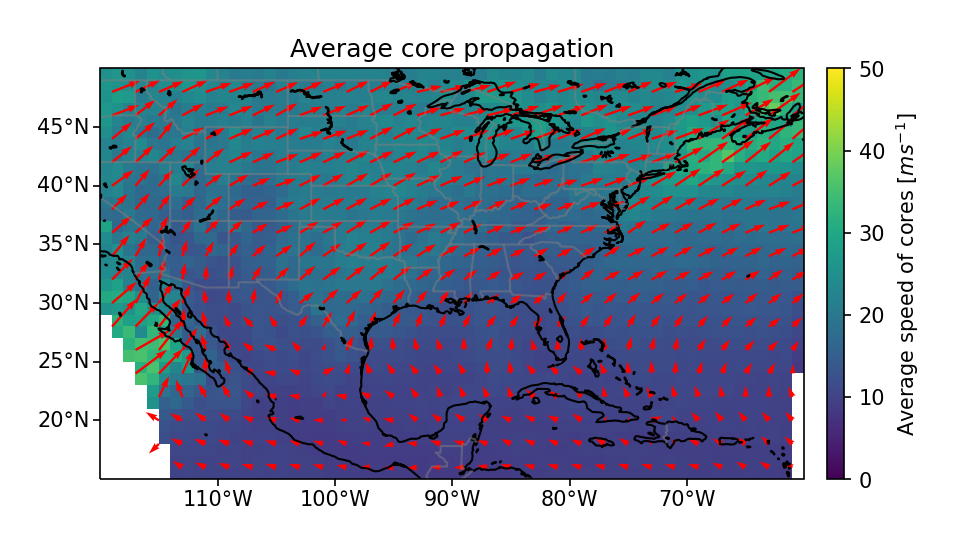
\includegraphics[width=0.75\textwidth]{figures/chapter2_10.png}
    \caption[
    Average core lifetime and minimum \acrshort{bt} with increasing core cooling rate
    ]{
    Average core lifetime (a) and minimum \acrshort{bt} (b) with increasing core cooling rate. Error bars show the standard error of the mean, and are large enough to the visible only for the largest cooling rates.
    }
    \label{fig:core_cooling_rate_relations}
\end{figure}


Figure~\ref{fig:core_cooling_rate_relations}\,a compares how the average lifetime of detected cores changes with their maximum observed cooling rate.
The observed core cooling rates range from 0.5\,K$\mathrm{\cdot minute^{-1}}$ to 4\,K$\mathrm{\cdot minute^{-1}}$, representing cloud top growth rates between 1.25\,\unit{ms^{-1}} to 10\,\unit{ms^{-1}}.
For low values of core cooling rate, there is a similar, positive linear relationship between cooling rate and lifetime between all regions, indicating that more intense convection leads to longer periods of cores being observed.
However, beyond cooling rates of around 1.5\,\unit{K minute\textsuperscript{-1}} there is a peak in the core intensity--height relationship, with larger cooling rates leading to shorter lifetimes.
This may be explained that the cores with faster cooling rates reach their level of neutral buoyancy faster, and therefore show cooling cloud tops for a shorter time period.
The inflexion in the core lifetime may also explain why there are no apparent differences in average lifetime between different regions, despite differences in other convective properties.

Figure~\ref{fig:core_cooling_rate_relations}\,b shows how the minimum \acrshort{bt} changes with the maximum cooling rate of the core.
Unlike fig.~\ref{fig:core_cooling_rate_relations}\,a, there is a continuous decrease in \acrshort{bt} with core cooling rate, indicating that faster cooling rates tend to result in cores with colder \acrshort{ctt} and hence higher \acrshort{cth}.
Figure~\ref{fig:core_cooling_rate_relations}\,b also provides context for the results seen in fig.~\ref{fig:core_cooling_rate_relations}\,a.
If it is assumed that cores are detected around the freezing level (273\,\unit{K}), then the overall temperature change over the core lifetime ranges from $\sim$45\,\unit{K} for the least intense cores to $\sim$65\,\unit{K} for the most intense cores.
Although this continues to increase with the cooling rate, the proportional change is less than that of the core cooling rate itself.
As the core lifetime can be approximated as the core \acrshort{bt} change divided by the cooling rate, the larger proportional change in cooling rate will result in a shorter lifetime for more rapidly cooling cores.

By multiplying the average core lifetime by the vertical velocity estimation from the cooling rate, an estimate for the convective layer height be can found.
For the longest lived cores with cooling rates around 1.5\,K$\mathrm{\cdot minute^{-1}}$ this results in an estimated convective layer height of 6.3\,km.
Using the moist pseudo-adiabatic lapse rate a total temperature difference across the observed lifetime of these cores can be calculated as 38\,K., resulting in an average initial detection temperature of approximately 255\,K.
For the most intense observed cores, with cooling rates greater than 3\,K$\mathrm{\cdot minute^{-1}}$ (7.5\,\unit{ms^{-1}}), the convective layer height is estimated as 11\,km, resulting in an initial temperature of 270\,K.
While in both cases the estimate for the initial temperature of observations is above the freezing level, this still agrees with the explanation for the inflexion in the growing core lifetime proposed in the previous paragraph.
Beyond a certain intensity, the lifetime of the growing phase of a convective core is constrained more by the convectively active layer height than the updraft intensity.

\subsection{Diurnal cycle of convective cores}

%f
\begin{figure}[tp]
    \centering
    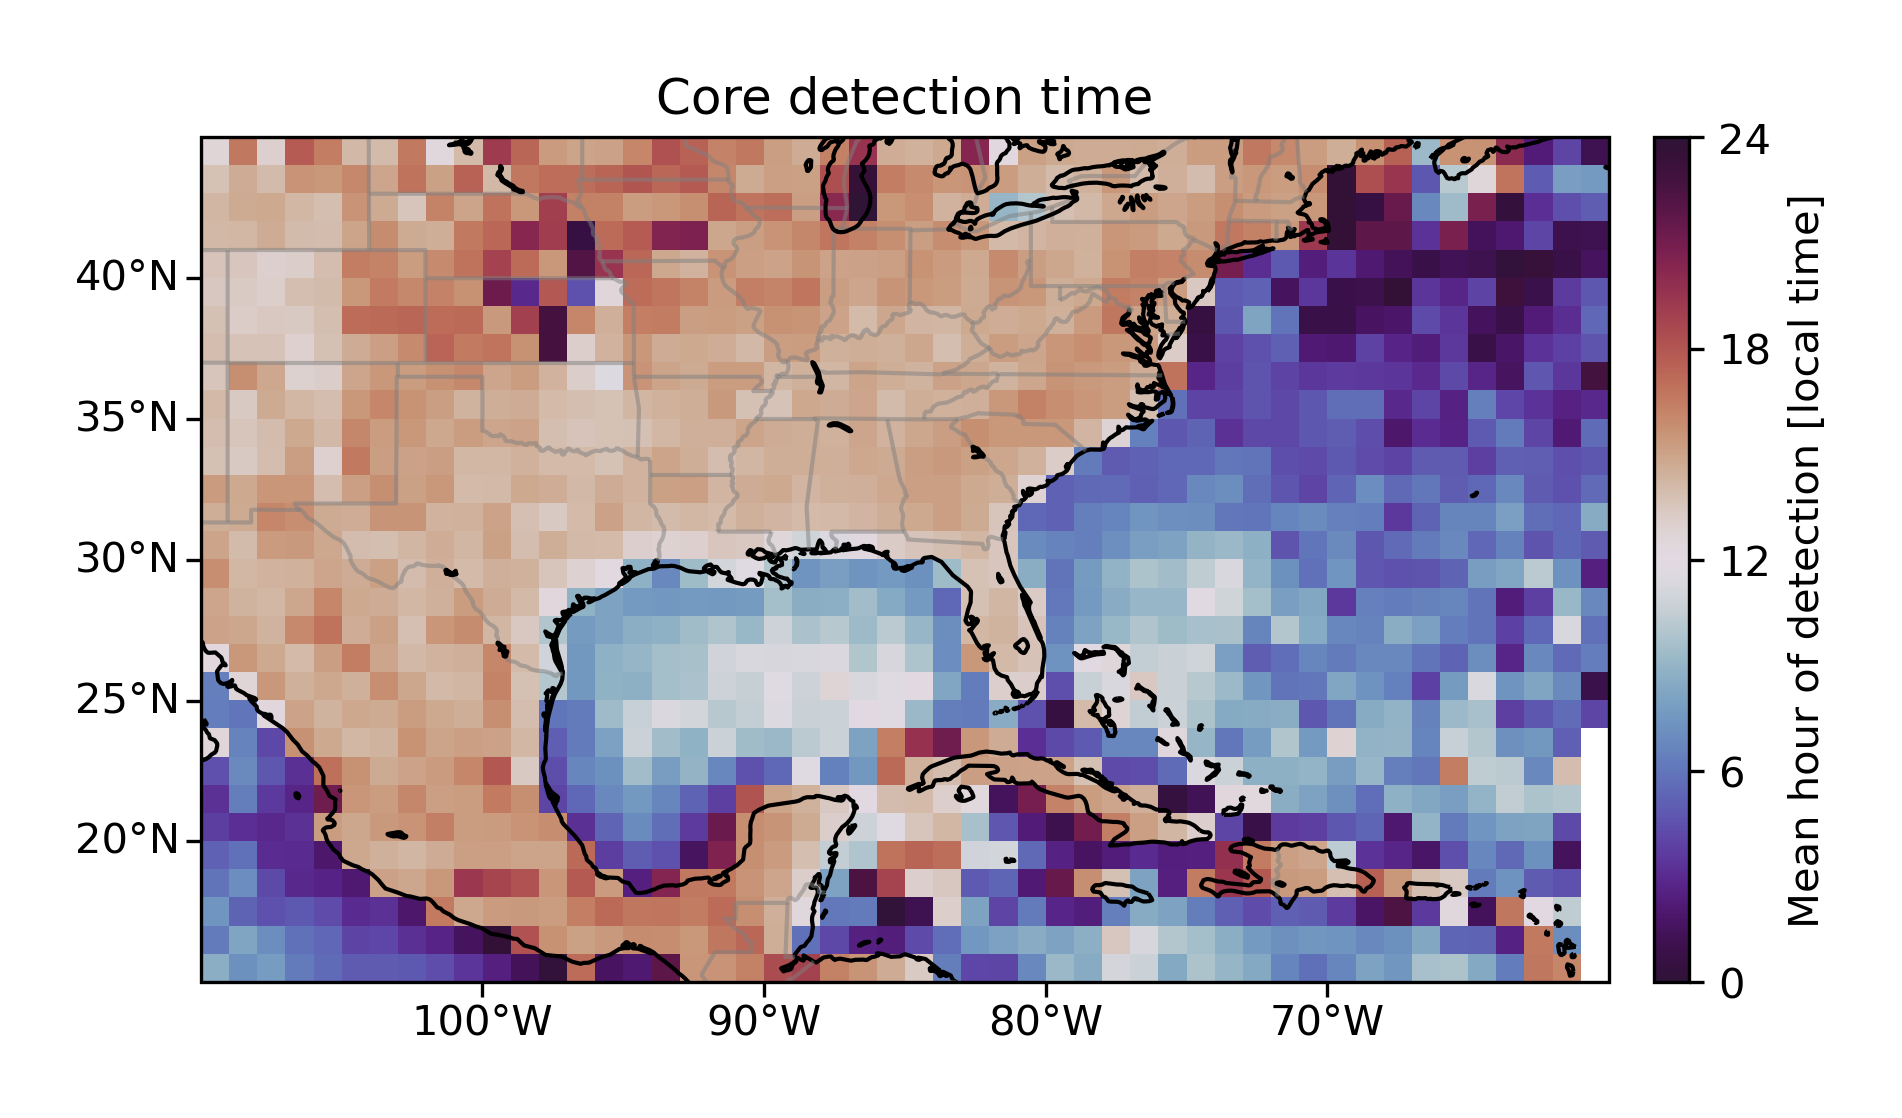
\includegraphics[width=\textwidth]{figures/chapter2_11.png}
    \caption[
    A map of the average time of day of initiation of detected cores
    ]{
    The average time of day of initiation of cores observed within each 1\texttimes1\textdegree\ grid box. The time of initiation is calculated as the local solar time based on longitude, and the mean is calculated as the circular mean over a 24-hour period to account for the cyclical aspect of the hour of day.
    }
    \label{fig:core_detection_time_map}
\end{figure}

Figure~\ref{fig:core_detection_time_map}, shows the mean time of detection for cores detected within each 1-degree grid square.
The most notable feature in fig.~\ref{fig:core_detection_time_map} is the strong land-sea contrast, with the majority of land regions showing convective activity occurring during the afternoon, and the majority of ocean regions showing activity before midday.
In addition, there are a few major features of the detected time of initiation across both land and sea regions.
In coastal regions in the Gulf of Mexico and the Caribbean Sea, earlier initiation times are seen closer to coastlines, while regions further from land have average times of detection closer to midday.
Over land there is also a later time of initiation over the Northern Great Plains (90--100\,\textdegree W, 37--47\,\textdegree N).

% \subsubsection{Regional differences in the time of core detection}


%f
\begin{figure}[tp]
    \centering
    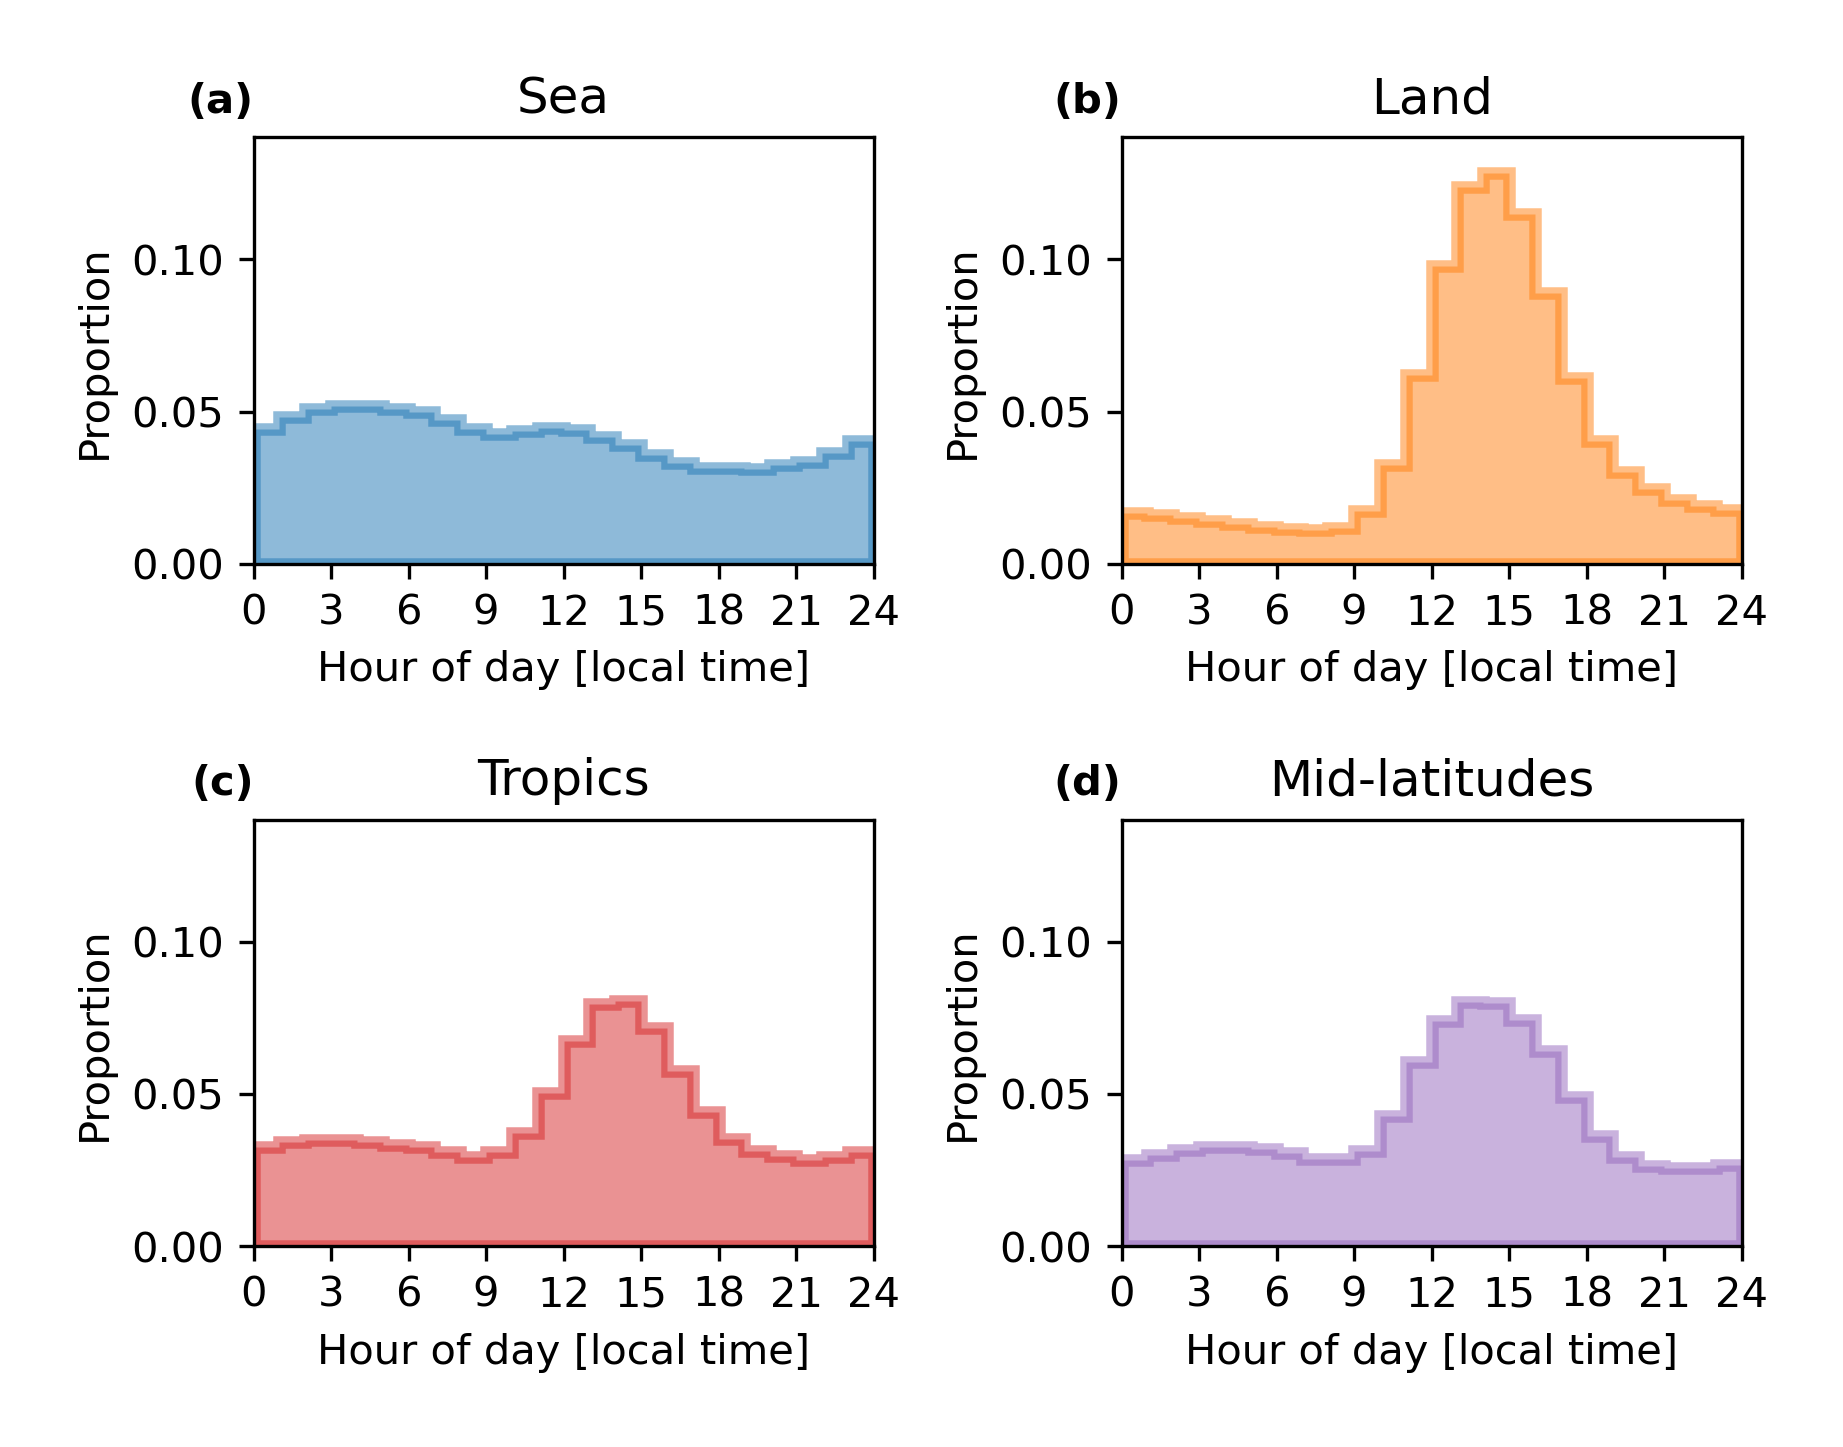
\includegraphics[width=\textwidth]{figures/chapter2_12.png}
    \caption[
    The diurnal distributions of the local time of detection for cores detected over land, sea, tropics and mid-latitudes
    ]{
    The diurnal distributions of the local time of detection for cores, binned by hour detected over (a) sea, (b) land, (c) tropics (\textless 30\,\textdegree N) and (d) mid-latitudes (\textgreater 30\,\textdegree N).
    }
    \label{fig:core_diurnal_land_sea}
\end{figure}


Figure~\ref{fig:core_diurnal_land_sea} shows the distribution of core detections across the diurnal cycle for land, sea, tropics and mid-latitude regions.
Over land there is a sharp peak in convective activity initiating in the mid-afternoon between 2 and 3 pm, with a tail extending into the night-time.
Over the sea, the distribution of core detections is much more uniform across the diurnal cycle.
There is still a peak observed in the early hours of the morning (3--6\,am), and a low in the evening (6\,pm), but the difference between these is much less pronounced than that over land.
Both the tropics and mid-latitudes have peaks in convection at the same time as that seen for all land regions in fig.~\ref{fig:core_diurnal_land_sea}\,b.
The peak for mid-latitudes is slightly broader, with more convection occurring later in the day.

%f
\begin{figure}[tp]
    \centering
    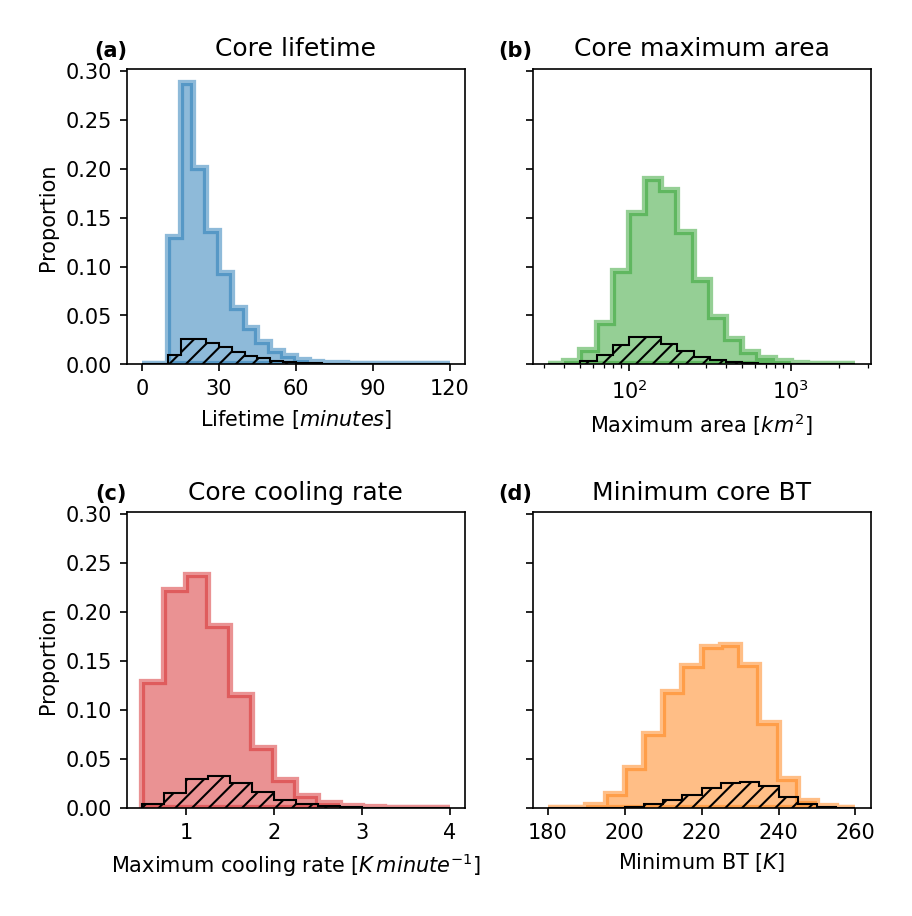
\includegraphics[width=0.75\textwidth]{figures/chapter2_13.png}
    \caption[
    The diurnal distribution of cores detected in the \acrshort{ngp} region
    ]{
    The diurnal distribution of cores detected in the \acrshort{ngp} region (37--45\,\textdegree\,N, 90--100\,\textdegree\,W).
    }
    \label{fig:core_ngp_contrast}
\end{figure}

Figure~\ref{fig:core_detection_time_map} showed a noticeably later average time of detection over the \acrfull{ngp} region.
Figure~\ref{fig:core_ngp_contrast} shows how the diurnal distribution of core detection time varies within this area, which is defined as 37--45\,\textdegree\,N, 90--100\,\textdegree\,W.
In contrast to the distribution seen over all land regions in fig.~\ref{fig:core_diurnal_land_sea}\,b, the \acrshort{ngp} region shows a later peak of convective activity between 3 and 4 pm, as well as much higher rates of convection observed during the nighttime and into the early morning until around 7\,am.
Previous studies have found a similar bimodal distribution in convective precipitation over the \acrshort{ngp} \citet{li_high-resolution_2021}.

%f
\begin{figure}[tp]
    \centering
    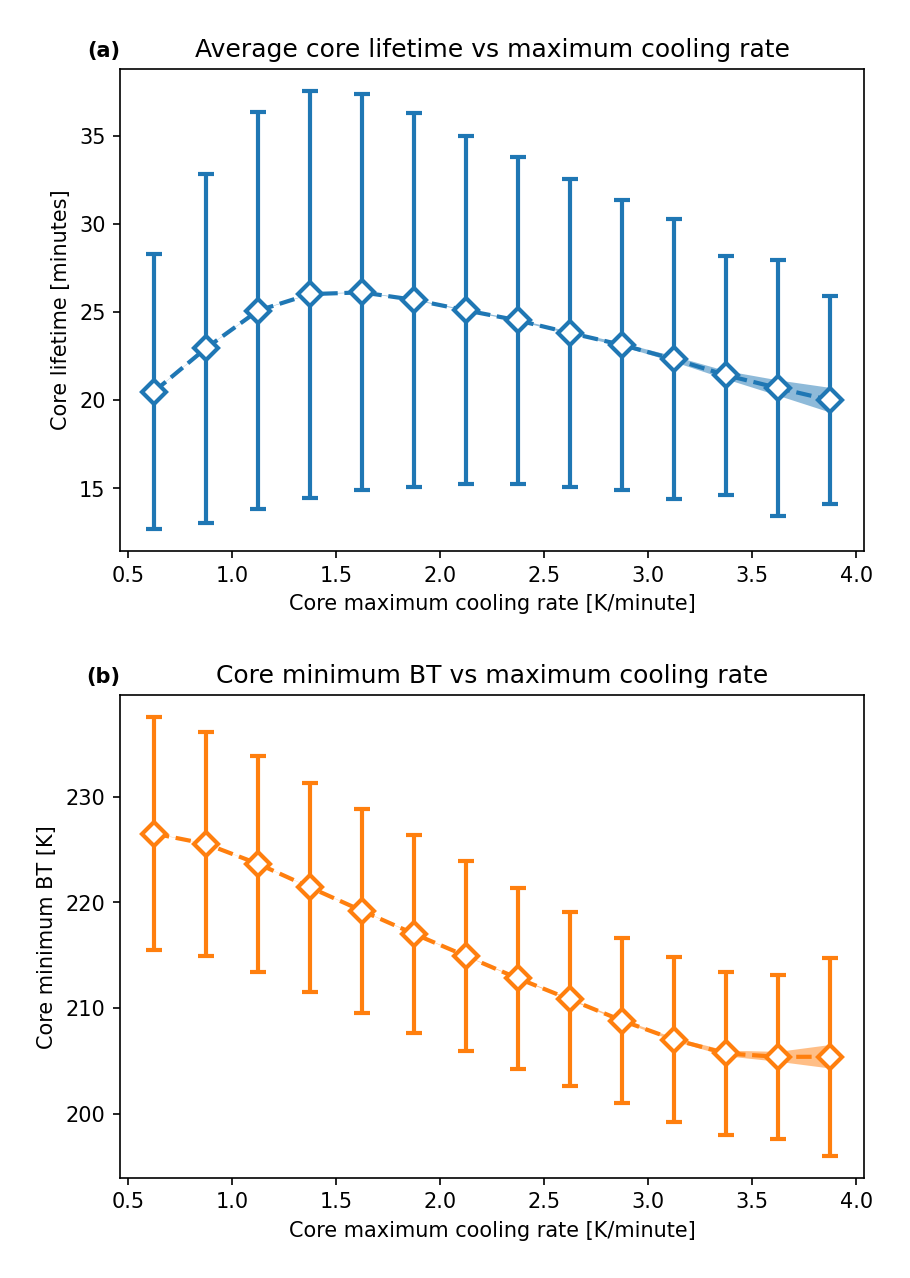
\includegraphics[width=0.75\textwidth]{figures/chapter2_14.png}
    \caption[
    The change in average time of core detection with distance from the coastline
    ]{
    The change in average time of core detection with distance from the coastline. Negative distances along the x axis show cores detected further to sea, and positive distances show cores detected further inland. Error bars are not shown as the standard error of the mean is too small to be visible.
    }
    \label{fig:core_coast_effect}
\end{figure}

In fig.~\ref{fig:core_coast_effect} the effect of the distance to the coast on core detection time is examined over the Gulf Coast region (22.5--32.5\,\textdegree\,N, 82.5--100\,\textdegree\,W).
Negative distances indicate locations further offshore, and positive distances those locations further inland.
Figure~\ref{fig:core_detection_time_map} showed a change in the average time of detection of cores in locations closer to the coast, and that effect is shown again here.
For cores detected over the sea, there is a linear decrease in the average time of detection as the distance to the coast increases.
For cores detected over land, there is a sharp decrease in the time of detection very close to the coast, although further than 50\,\unit{km} from the coast this becomes a shallower linear gradient.
The linear change of core detection time with distance from the coastline may be linked to offshore and onshore breezes triggering convection.
Cores over land see a reduction in the variance of the time of detection between 50 and 150\,\unit{km} from the coast, which may also indicate that an external forcing from sea breeze is triggering convection in these areas, constraining the time of initiation of convection.

%f
\begin{figure}[tp]
    \centering
    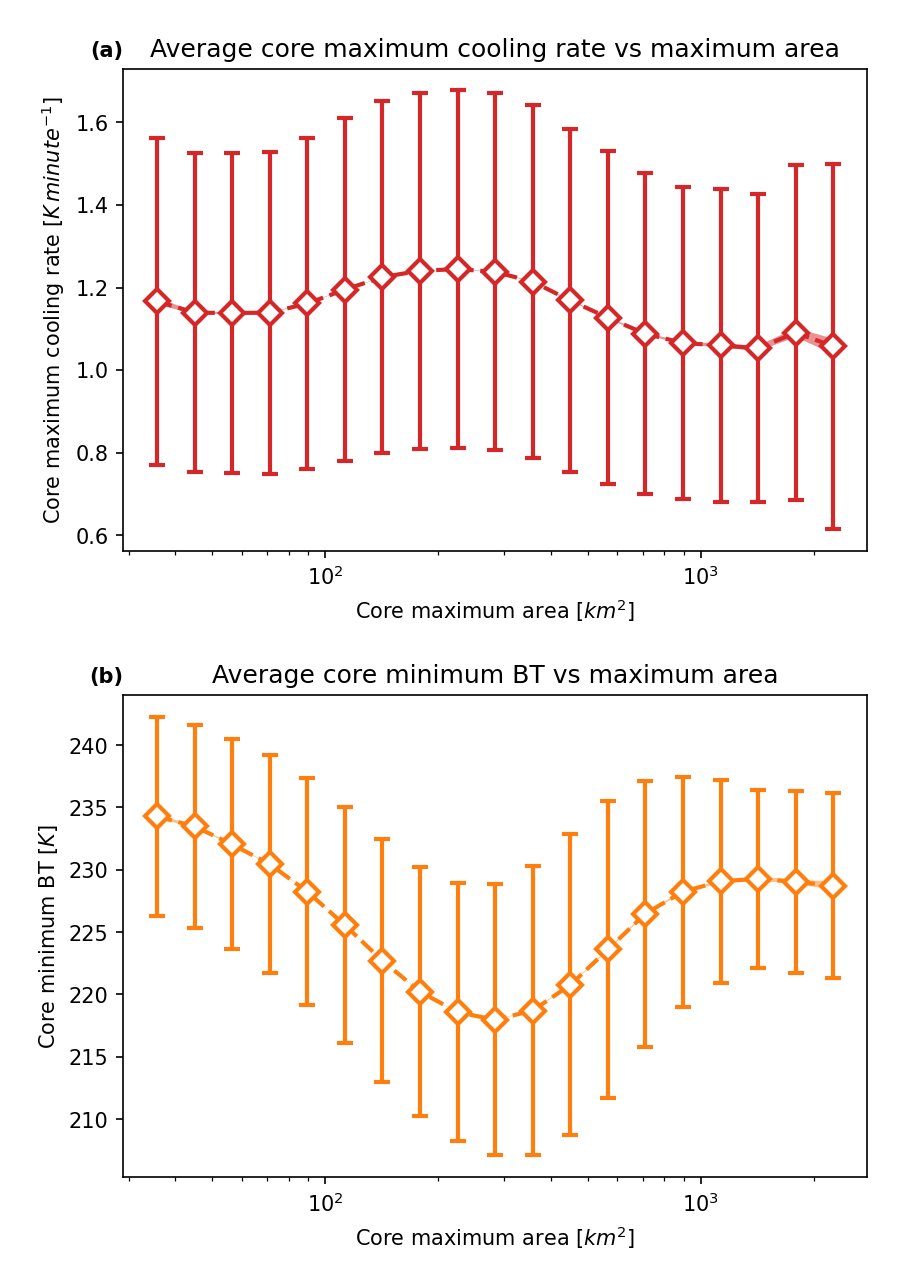
\includegraphics[width=\textwidth]{figures/chapter2_15.png}
    \caption[
    The diurnal cycle of the maximum cooling rate of cores detected over land, sea, tropics and mid-latitudes
    ]{
    The diurnal cycle of the maximum cooling rate of cores detected over (a) sea, (b) land, (c) tropics (\textless 30\,\textdegree N) and (d) mid-latitudes (\textgreater 30\,\textdegree N). Each point shows the mean of the maximum cooling rate of cores detected during that hour. Error bars are not shown as the standard error of the mean is too small to be visible.
    }
    \label{fig:core_diurnal_cooling_rate}
\end{figure}

Figure~\ref{fig:core_diurnal_cooling_rate} shows how the mean maximum cooling rate of cores changes across the diurnal cycle.
While over the sea there is little change in cooling rate, over land there is a noticeable increase in the cooling rate throughout the daylight hours.
This leads to a peak at around 4\,pm, before the cooling rate falls back to its nighttime levels which are lower than that seen over ocean.
Both tropics and mid-latitudes show similar diurnal cycles to land, albeit with a difference of 0.2\,\unit{K minute\textsuperscript{-1}} across the entire diurnal cycle.


\subsection{Distributions and properties of observed anvil clouds} \label{sec:anvil_properties}

In this section, the properties of anvil clouds in the dataset are examined.
Anvils are detected and tracked independently from cores.
Although anvils must be associated with observed cores at the start of their lifetime, tracking of anvils continues beyond the extent of the observed core lifetime.
This also allows the detection of anvils that are associated with multiple cores, providing insight into the effects of convective organisation on anvil properties.

%f
\begin{figure}[tp]
    \centering
    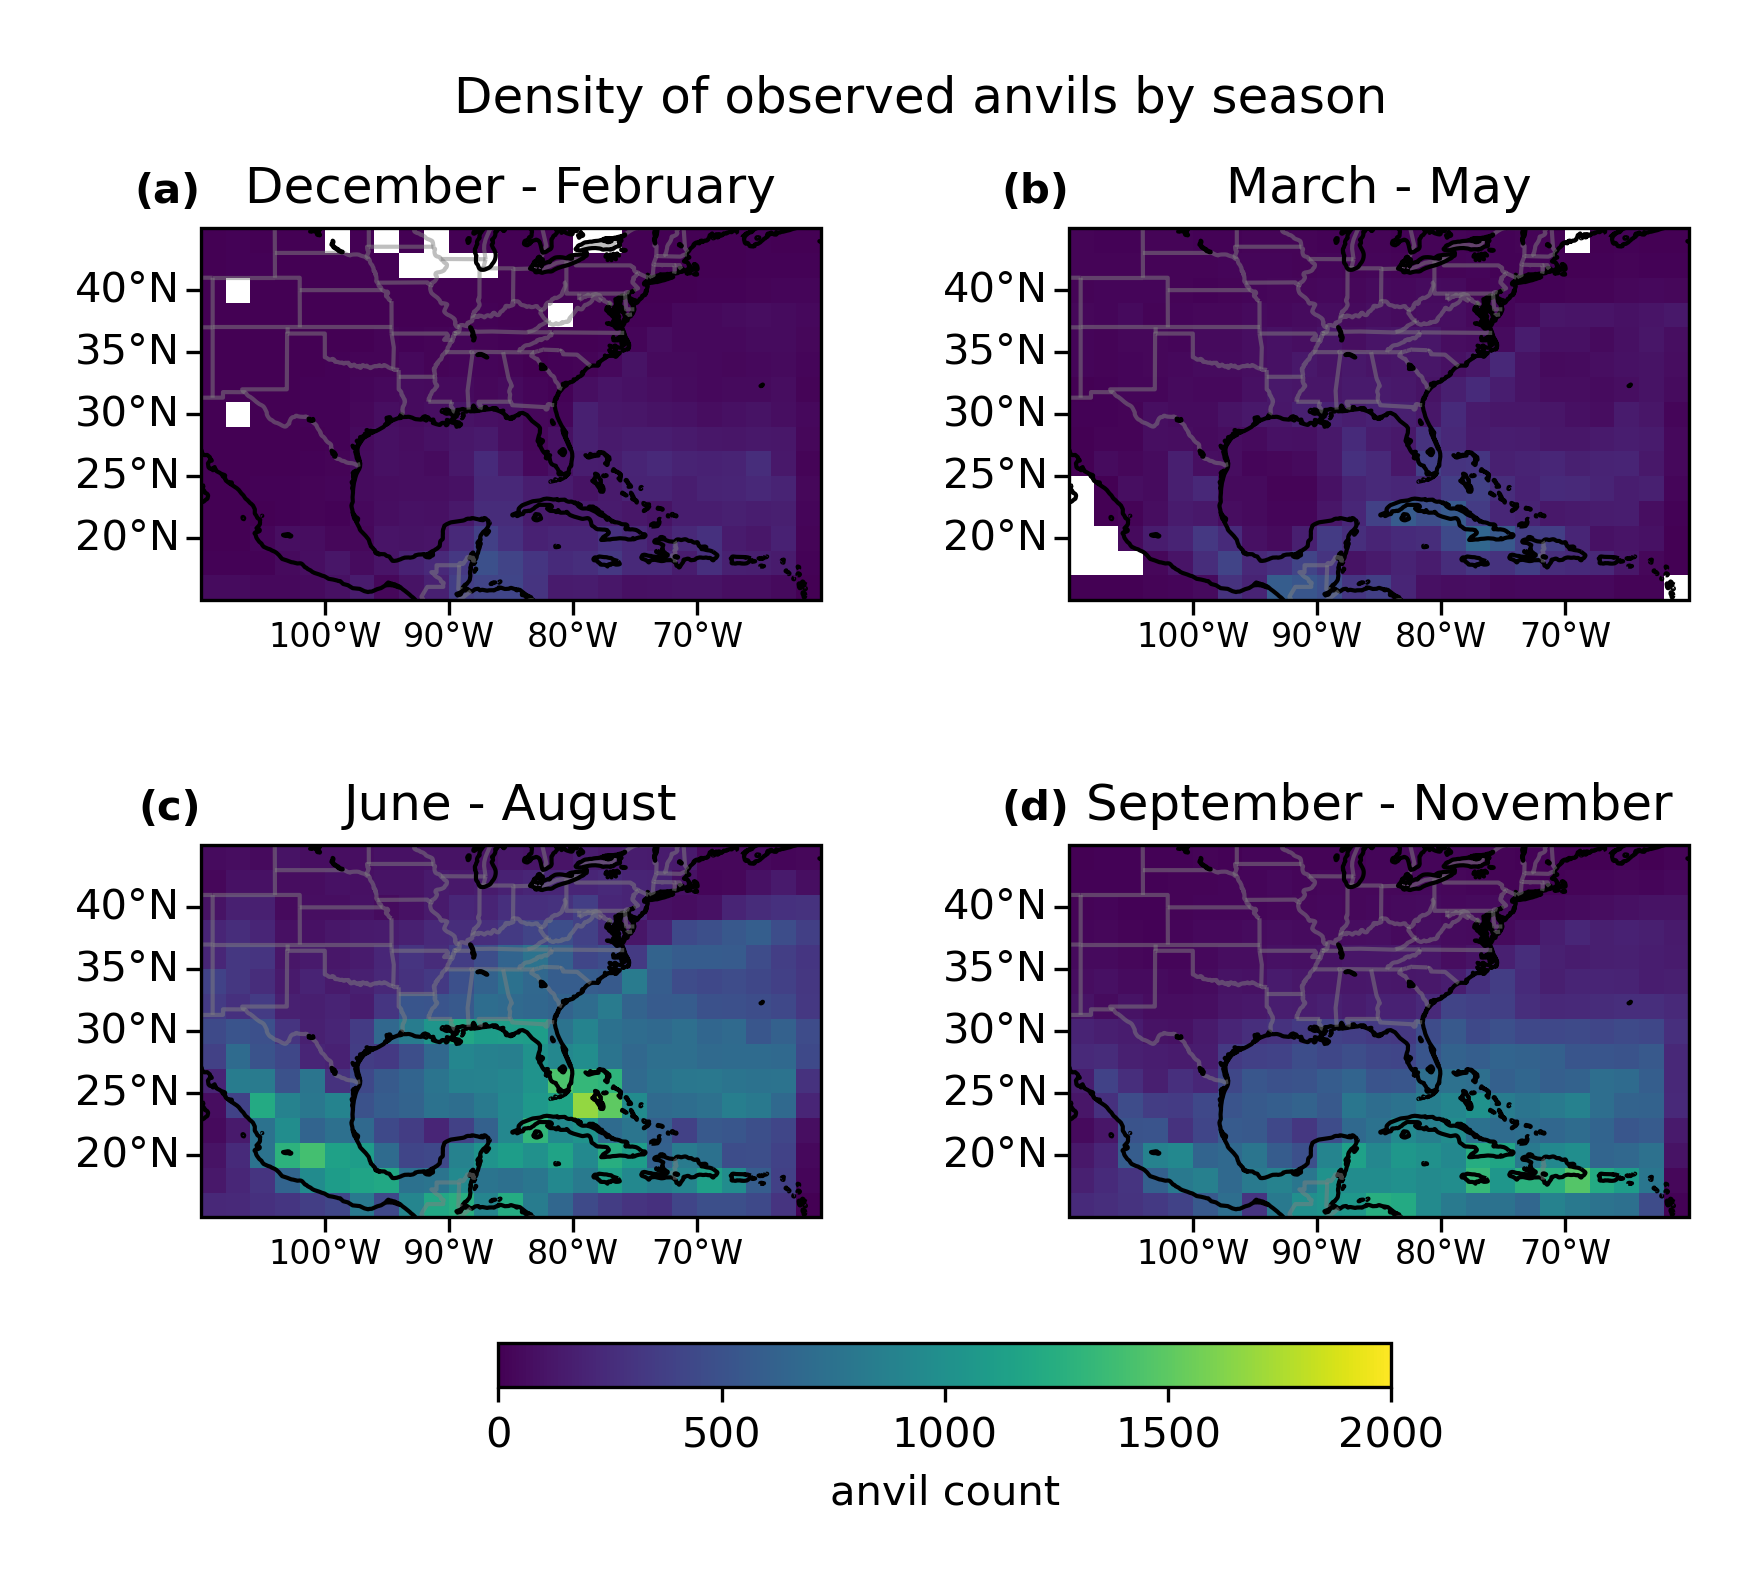
\includegraphics[width=\textwidth]{figures/chapter2_16.png}
    \caption[
    Maps showing the spatial distribution of observed anvils by season
    ]{
    Maps showing the spatial distribution of observed anvils for (a) winter, (b) spring, (c) summer and (d) autumn, each binned to a 2\texttimes2\,\textdegree grid.
    }
    \label{fig:anvil_distribution_map}
\end{figure}

Figure~\ref{fig:anvil_distribution_map} shows the counts of anvils for each 2\texttimes2\,\textdegree grid box, separated by season.
There is a similar seasonal cycle and distribution to fig.~\ref{fig:core_density_by_season}.
In winter (fig.~\ref{fig:anvil_distribution_map}\,a) and spring (fig.~\ref{fig:anvil_distribution_map}\,b) there are low rates of convection, with the majority of convection observed over warm ocean regions.
In summer, fig.~\ref{fig:anvil_distribution_map}\,c shows the highest rates of anvil detections, with a large increase in the observations of anvils over land.
In spring (fig.~\ref{fig:anvil_distribution_map}\,d), the number of anvils observed over the ocean remains high, but that over land reduces.

%f
\begin{figure}[tp]
    \centering
    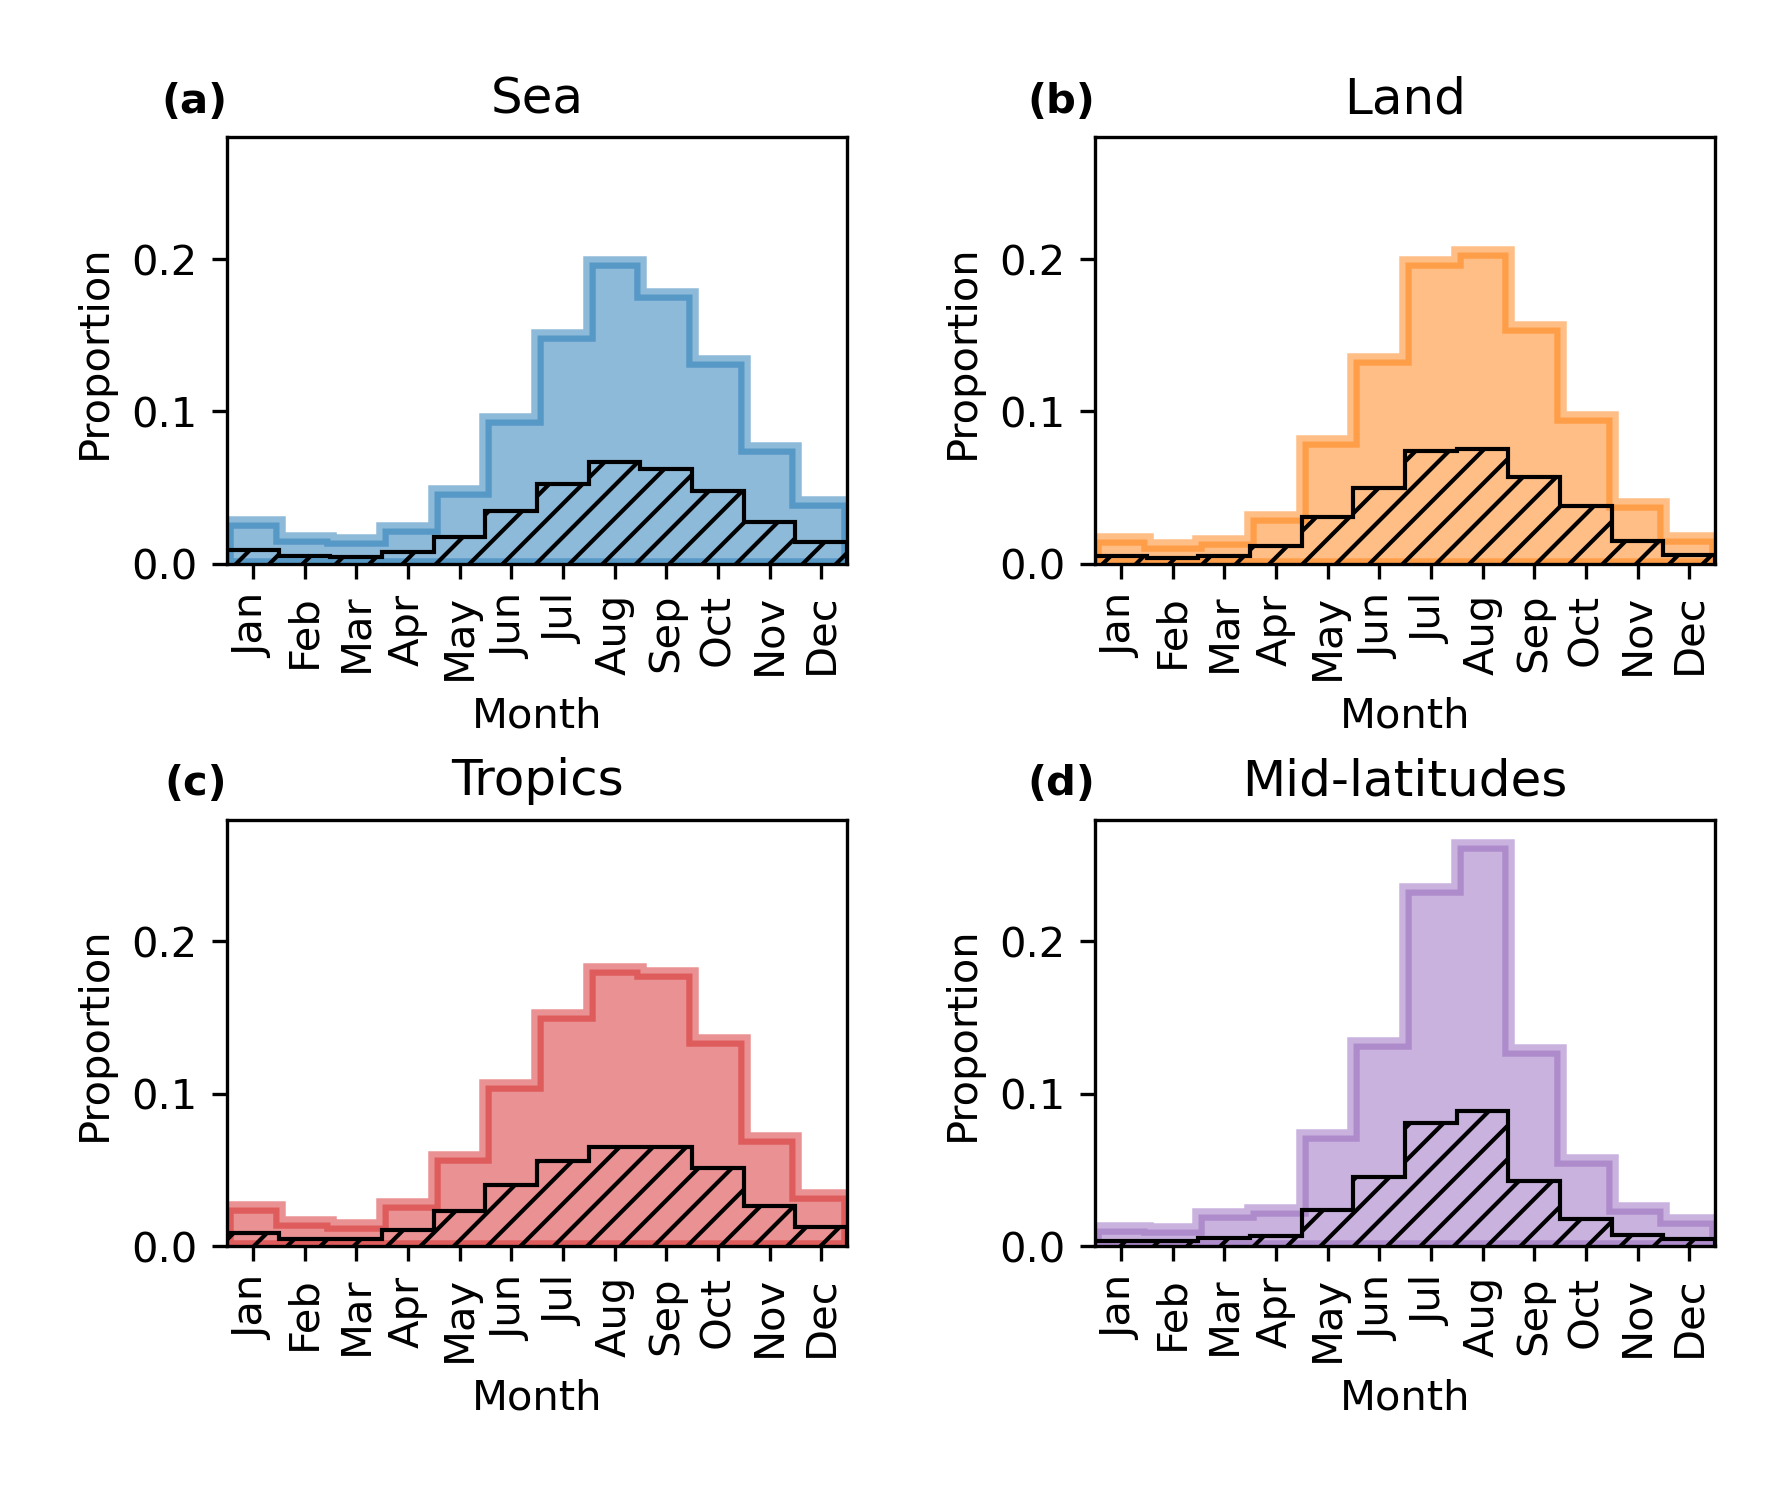
\includegraphics[width=\textwidth]{figures/chapter2_17.png}
    \caption[
    Monthly distributions of the proportion of anvils detected each month over land, sea, tropics and mid-latitudes
    ]{
    Monthly distributions of the proportion of anvils detected each month over (a) sea, (b) land, (c) tropics (\textless 30\,\textdegree N) and (d) mid-latitudes (\textgreater 30\,\textdegree N). The hatched area shows the proportion of the distribution consisting of anvils with multiple cores.
    }
    \label{fig:anvil_monthly_cycles}
\end{figure}

Figure~\ref{fig:anvil_monthly_cycles} shows how the annual distribution of anvil detections changes by month across different regions.
While similar to the annual distribution of cores shown in fig.~\ref{fig:core_annual_land_sea}, it shows a later peak over oceans in August--September compared to July--August over land.
The mid-latitudes have a sharper peak around these two months, while the tropics show a broader distribution of anvil detections throughout the year.


%f
\begin{figure}[tp]
    \centering
    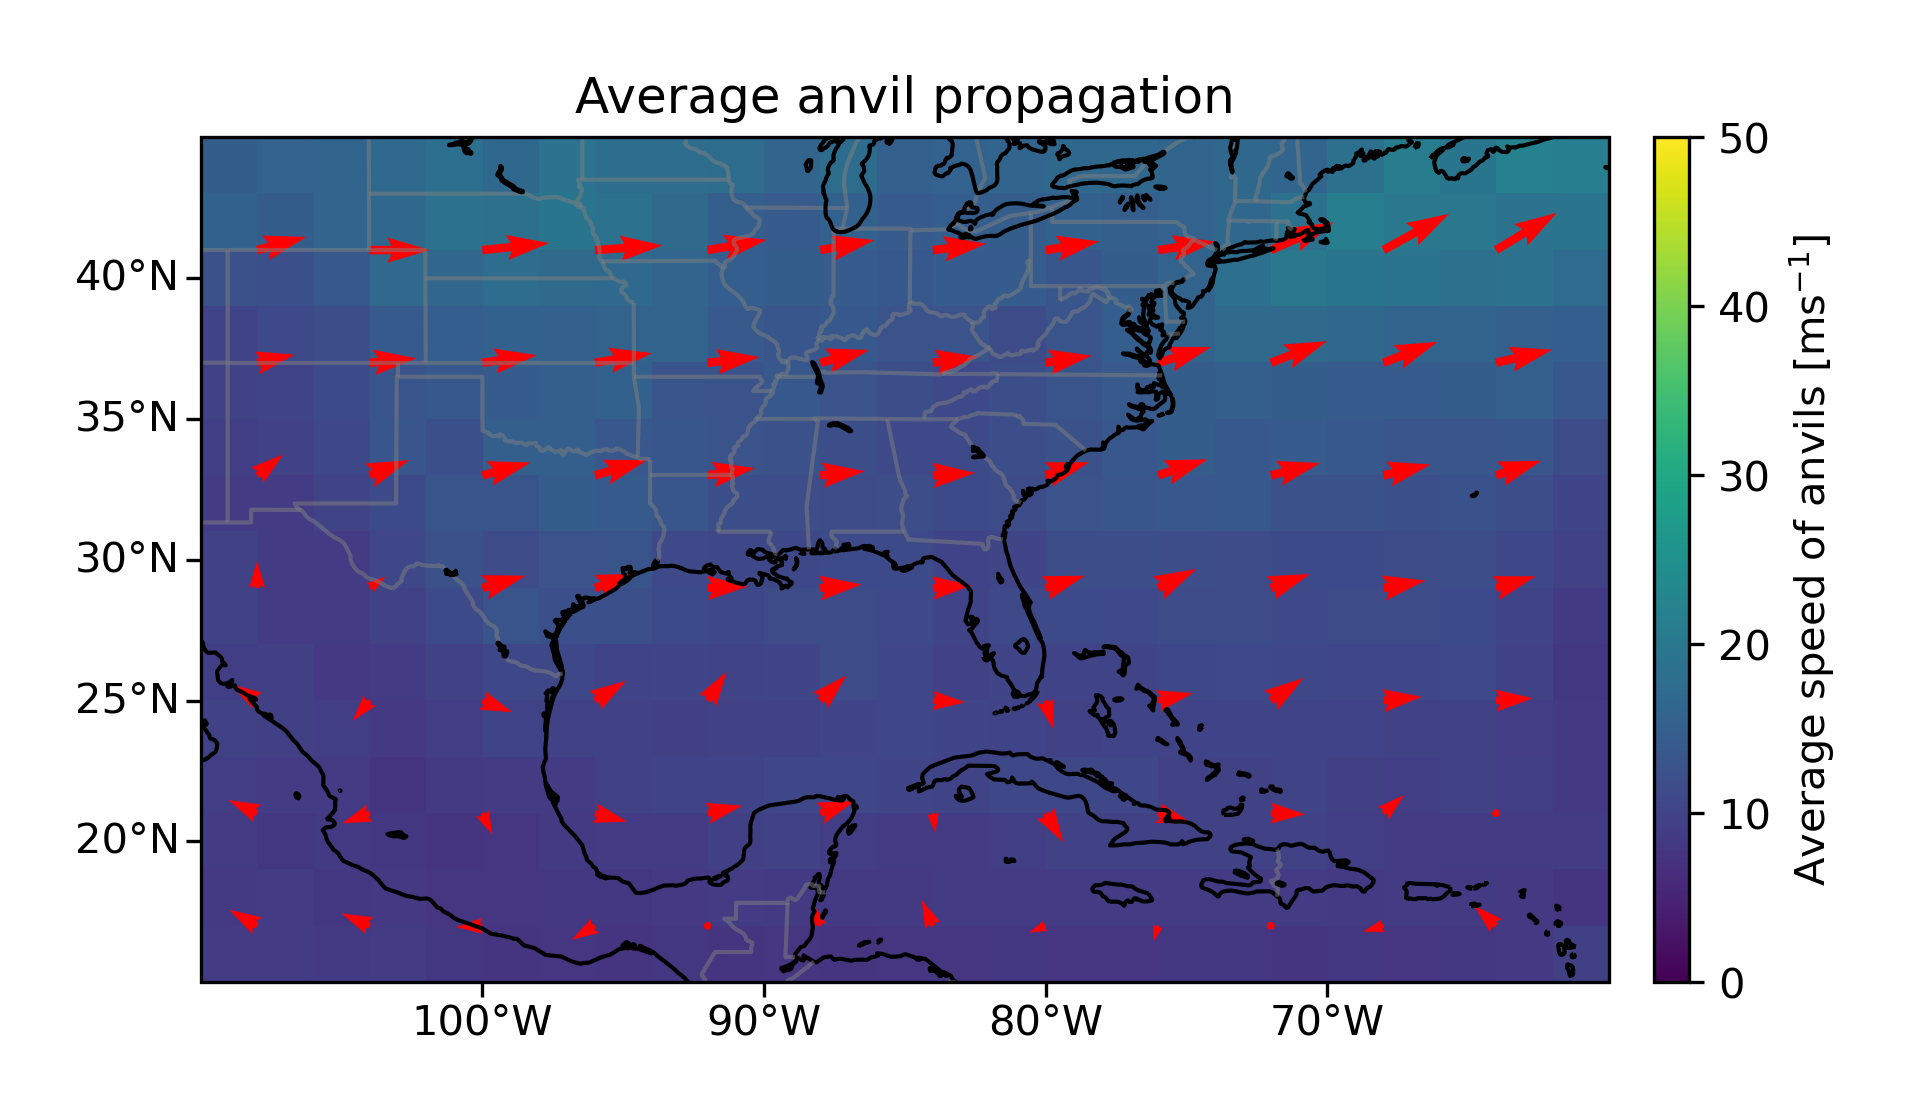
\includegraphics[width=\textwidth]{figures/chapter2_18.png}
    \caption[
    The average speed and direction of propagation of anvils
    ]{
    The average speed and direction of propagation of cores observed within each 2\texttimes2\textdegree\ grid box. The colouring shows the average speed of propagation, and the red arrows show the average direction of propagation for each 4\texttimes4\textdegree\ grid box
    }
    \label{fig:anvil_propagation_map}
\end{figure}

Figure~\ref{fig:anvil_propagation_map} shows the average propagation speed and direction for anvils in the same manner as shown for cores in fig.\ref{fig:core_propagation_map}.
In the extra-tropics (\textgreater30\,\textdegree\,N), there is generally a westerly motion, without the southerly motion seen in the cores.
This westerly motion corresponds to the prevailing high-level winds.
The change in direction and differences in the speed of propagation between anvils and cores indicates a typical shear between the two.
Over the tropics (\textless30\,\textdegree\,N) no clear overall motion of anvils is apparent.


%f
\begin{figure}[tp]
    \centering
    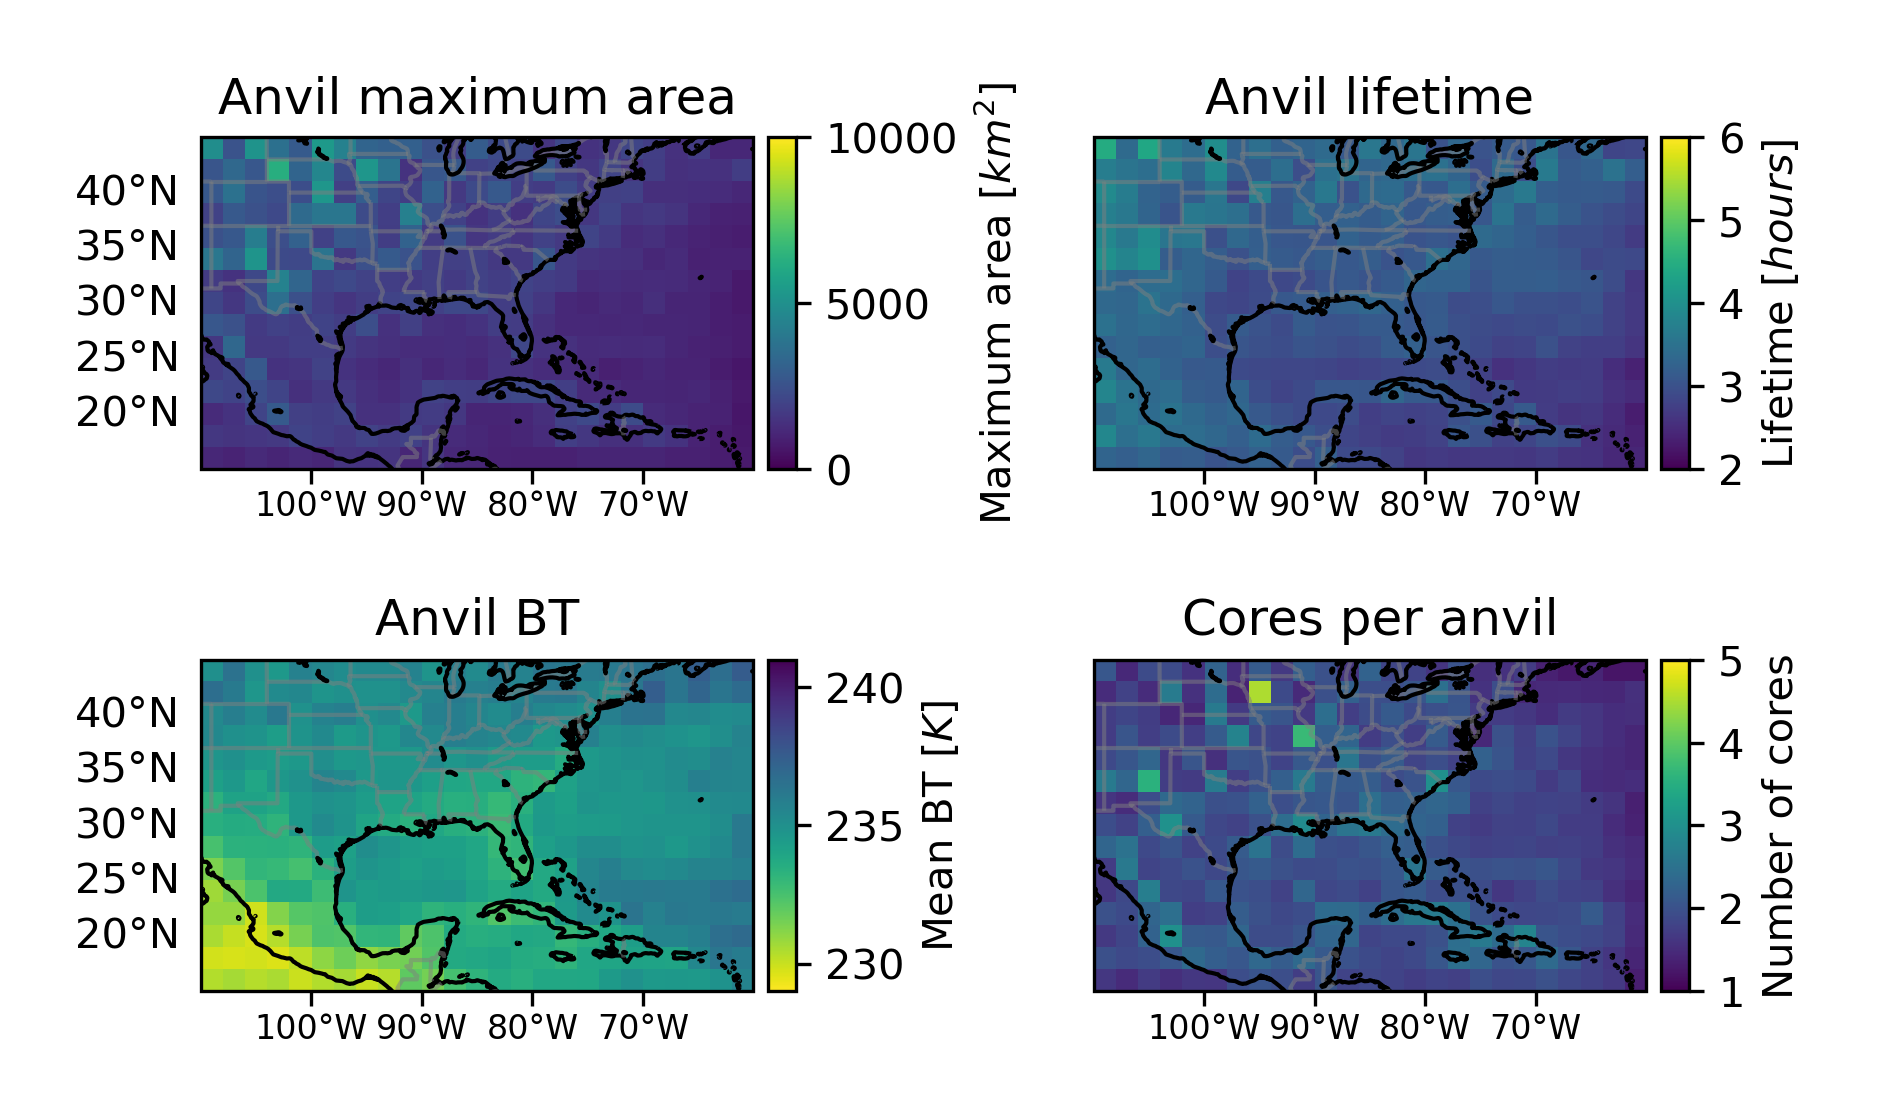
\includegraphics[width=\textwidth]{figures/chapter2_19.png}
    \caption[
    Maps showing the spatial changes in the averages of anvil maximum area, lifetime, \acrshort{bt} and number of cores
    ]{
    Maps showing the spatial changes in the averages of (a) anvil maximum area, (b) lifetime, (c) \acrshort{bt} and (d) number of cores, binned to a 2\texttimes2\,\textdegree grid.
    }
    \label{fig:anvil_properties_maps}
\end{figure}

Figure~\ref{fig:anvil_properties_maps} shows maps of the average anvil properties for the maximum area (a), lifetime (b), \acrshort{bt} (c), and number of cores (d) over each 2\texttimes2\,\textdegree grid box.
Both the anvil maximum area and lifetime increase towards the northwest corner of the domain.
While this may be due to the tendency of \acrshort{mcs}s to initiate East of the Rocky mountains \citep{feng_spatiotemporal_2019}, it may also be a sign of a systematic bias affecting the anvil areas.
Both the increase in average anvil area and lifetime shown in fig.~\ref{fig:anvil_properties_maps}\,a and b appear to correlate with the satellite zenith angle (fig.~\ref{fig:abi_zenith_angles}).
As the minimum core and anvil area requirement in the detection algorithm is determined by the number of pixels, the minimum area in \unit{km^2} will increase with the zenith angle.
As the anvil lifetime tends to correlate with the maximum area, this zenith angle bias may contribute to the patterns seen in both fig.~\ref{fig:anvil_properties_maps}\,a and b.

The average anvil \acrshort{bt} becomes colder towards the southwest of the domain, while the average number of cores per anvil are too variable to see any clear spatial trends.
As very large \acrshort{mcs}s with many cores are both rare and large outliers, they introduce a large amount of variability into the average number of cores per anvil when gridded by the initiation location.

% There is again a land--sea contrast in the Caribbean and Gulf of Mexico.
% The most notable change is the increase in anvil area towards the North--West of the domain.
% This correlates with the change in sensor zenith angle---and hence the area of each pixel---shown in fig.~\ref{fig:abi_zenith_angles}.
% It is possible that there is a bias towards observing larger anvils due to the larger pixel area at larger zenith angles.
% However, previous studies have shown that this region is where most \acrshort{mcs}s in North America originate from \citep{feng_spatiotemporal_2019} which may also explain the large average areas.

% Figure~\ref{fig:anvil_properties_maps}\,b shows the average anvil lifetime (in hours) for each 2\texttimes2\,\textdegree grid box.
% There is a similar, but smaller, trend towards longer-lived anvils in the North-West of the domain as that seen for the anvil area in fig.~\ref{fig:anvil_properties_maps}\,a.
% In addition, there is a tendency for average lifetimes over the ocean to be shorter than adjacent land regions.

% Figure~\ref{fig:anvil_properties_maps}\,c shows the average \acrshort{bt} of anvils in each grid box.
% Increasing latitude shows an increase (warming) of \acrshort{bt} over land.
% In addition, there is a land--sea contrast, with warmer \acrshort{bt} over sea than land.
% The coldest average \acrshort{bt} are observed over the Western coast of Mexico.

% Figure~\ref{fig:anvil_properties_maps}\,d shows the average number of cores associated with each anvil in each grid box.
% The Caribbean shows a noticeable land--sea contrast with an increase in the average number of cores over land, indicating that there is greater organisation of convection occurring there compared to over the sea.
% For the majority of land regions the average is reasonably noisy.
% This is primarily due to the presence of a small number of very large systems (including \acrshort{mcs}s), which have a very large number of cores and hence introduce noise to the spatial average.
% In addition, there is see a reduction in the average number of cores towards the edge of the map which is likely due to larger anvils being more likely to be removed from the dataset by the criteria in table~\ref{table:anvil_validity_criteria}.

%f
\begin{figure}[tp]
    \centering
    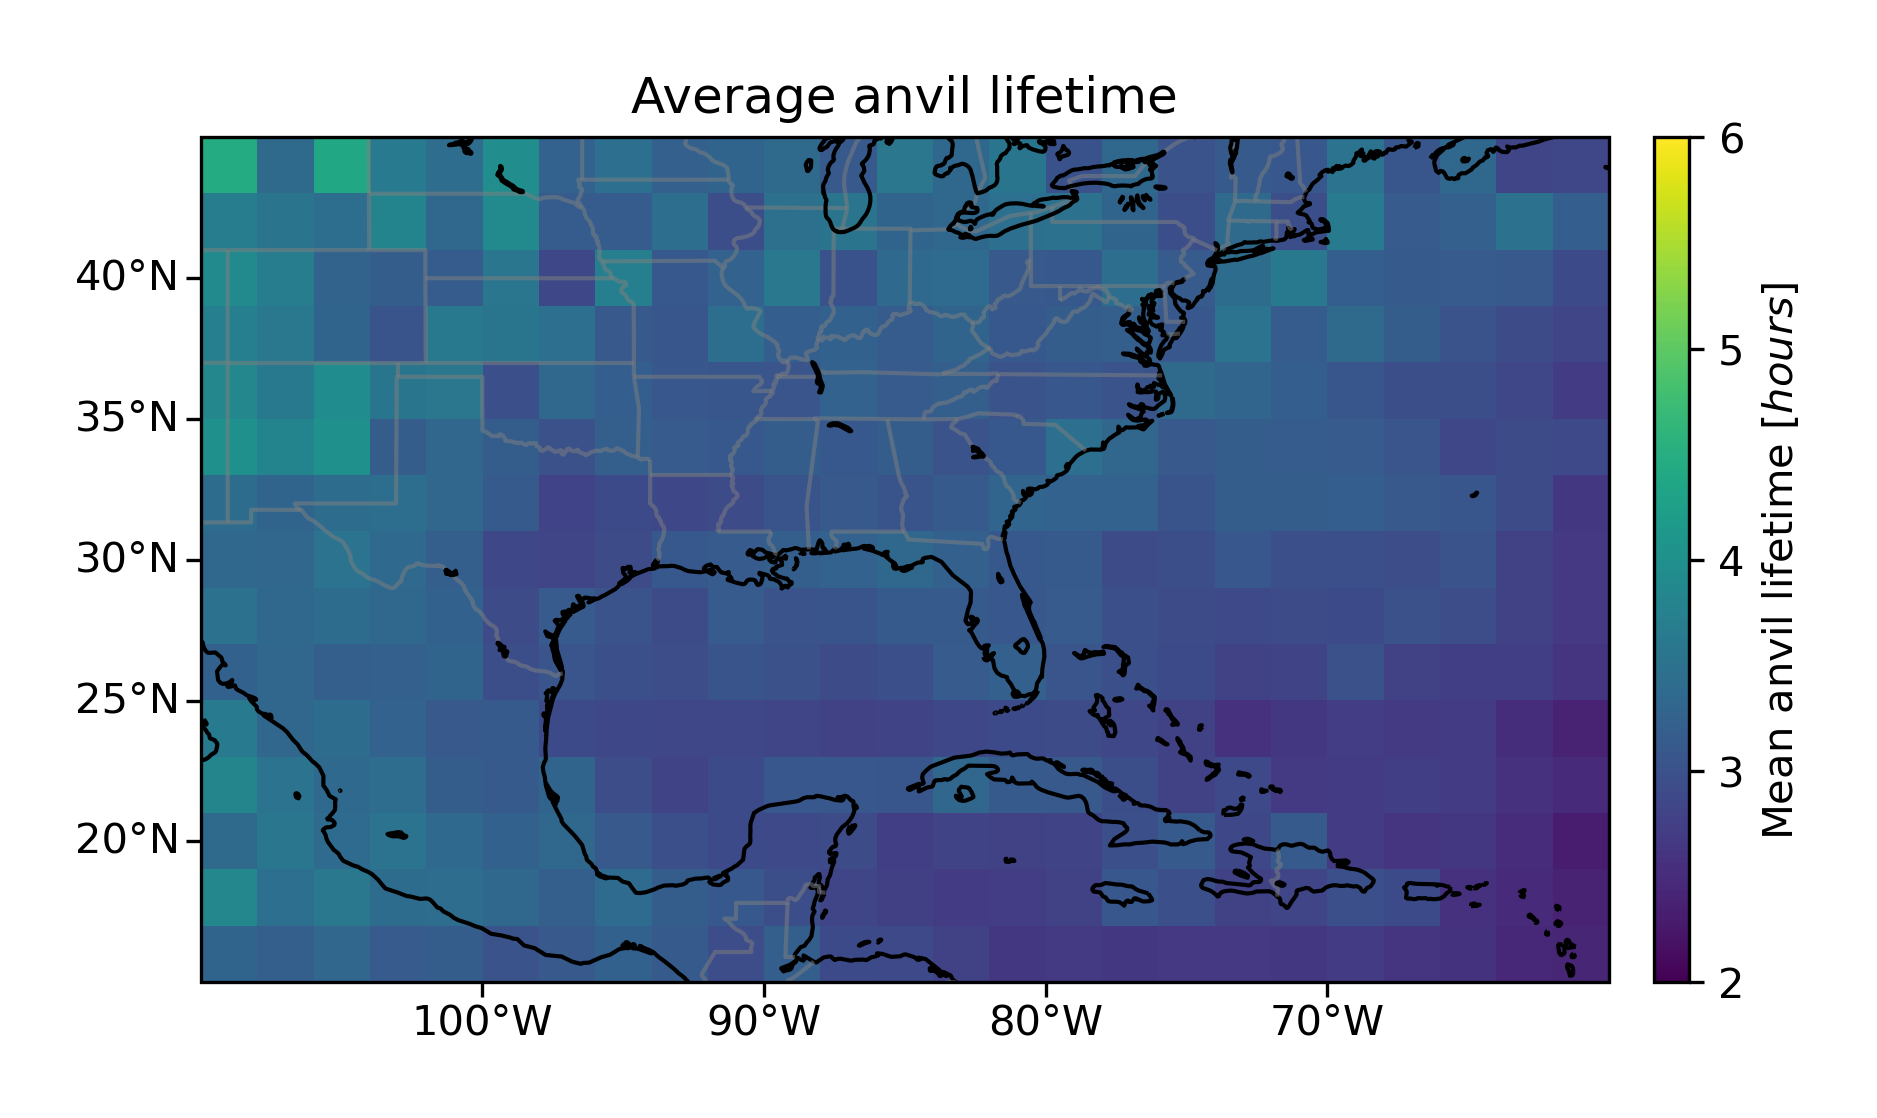
\includegraphics[width=0.9\textwidth]{figures/chapter2_20.png}
    \caption[
    Histograms showing the distribution of observed anvil properties
    ]{
    Histograms showing the distribution of observed anvil properties, with the hatched area showing the proportion associated with multiple core anvils. (a) The maximum area of the thick anvil cloud; (b) the maximum area of the thin anvil cloud (which includes both the thick and thin anvil regions; (c) the lifetime of the thick anvil and (d) the thin anvil; and (e) the average and (f) minimum observed \acrshort{bt} within each anvil.
    }
    \label{fig:anvil_properties}
\end{figure}

Figure~\ref{fig:anvil_properties} shows the distributions of anvil properties, with the proportion consisting of multiple-core anvils shown by the hatched area.
The anvil maximum area distribution has a similar shape for both thick anvils (fig.~\ref{fig:anvil_properties}\,a) and thin anvils (fig.~\ref{fig:anvil_properties}\,b), with the mean shifted to large values for the thin anvil.
It should be noted that the thin anvil area includes that of both thick and thin anvil regions, so will always be larger than that of the thick anvil alone.
The anvil lifetime distributions for the thick (fig.~\ref{fig:anvil_properties}\,c) and thin (fig.~\ref{fig:anvil_properties}\,d) anvils show a similar relationship, with a shift of the distribution to longer lifetimes for the thin anvil.
In both cases, despite the log scaling on the x-axis, there is a long tail towards larger area values and longer lifetimes.
Furthermore, this large tail consists primarily of multiple-core systems, as shown by the hatched area, indicating the impact of organisation on the area and lifetime of \acrshort{dcc}s.

Figure~\ref{fig:anvil_properties}\,e and fig.~\ref{fig:anvil_properties}\,f show the average and minimum anvil \acrshort{bt} over each detected anvil.
The minimum anvil \acrshort{bt} has a broader distribution than that of the average anvil \acrshort{bt}.
Multiple core anvils generally have colder anvil \acrshort{bt}, particularly so for the minimum \acrshort{bt}.
The cold tail of the minimum \acrshort{bt}, with values less than 200\,\unit{K}, indicates the presence of overshooting tops within these organised systems.

%f
\begin{figure}[tp]
    \centering
    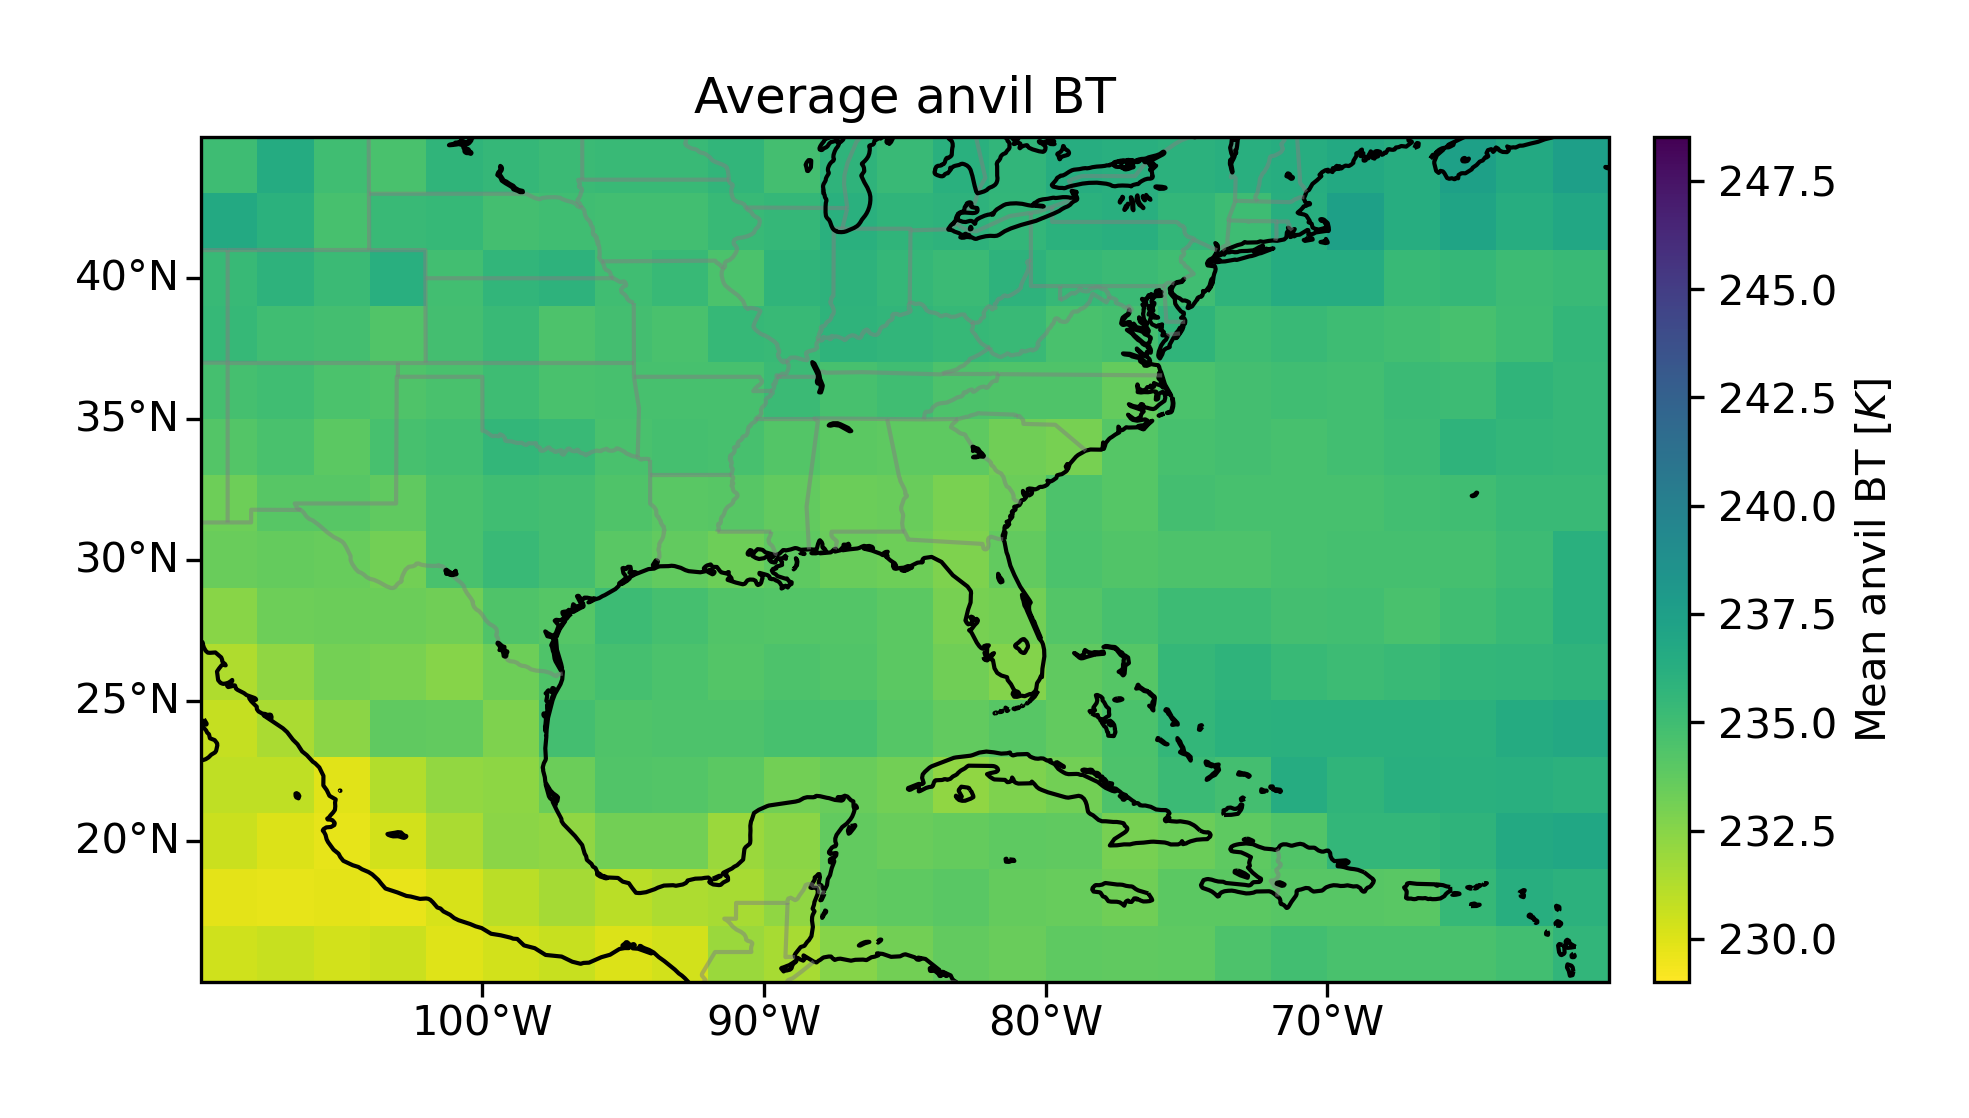
\includegraphics[width=0.9\textwidth]{figures/chapter2_21.png}
    \caption[
    The change in the average area and lifetime of anvils with different number of cores, and their total area coverage.
    ]{
    The change in the average area and lifetime of anvils with different number of cores. Mean values of (a) maximum thick anvil area, (b) maximum thin anvil area, (c) thick anvil lifetime and (d) thin anvil lifetime all increase with increasing number of cores. (e) The proportion of all anvils with different numbers of cores and (f) the fraction of total anvil coverage attributed to those anvils.}
    \label{fig:anvil_cores_and_coverage}
\end{figure}

Figure~\ref{fig:anvil_cores_and_coverage}\,a, b, c and d the average of the thick anvil maximum area, thin anvil maximum area, thick anvil lifetime and thin anvil lifetime for anvils with different numbers of cores.
In all cases these areas and lifetimes increase with an increasing number of cores.
In particular, the increase in the number of cores has a large impact on the maximum area of anvils, 
The most organised systems, which contain 10 or more cores, have areas that are more than two orders of magnitude greater on average than the anvils of isolated \acrshort{dcc}s.

Figure~\ref{fig:anvil_cores_and_coverage}\,e and f show the distribution of the number of cores associated with each detected anvil, and the proportion of total anvil coverage attributed to anvils with different core counts respectively.
Overall, the vast majority of anvils detected are isolated \acrshort{dcc}s with only a single core.
For anvils with greater than five cores, the number of systems observed drops to such a level that grouping of these \acrshort{dcc}s into bins of 6--9 cores and 10 or more is performed to ensure that there is a representative sample size of each group.
Despite making up the majority of observed \acrshort{dcc}s, single core systems only make up 12\% of the total anvil coverage.
Instead, despite being few in number, the most organised \acrshort{dcc}s with ten or more cores are responsible for the majority of anvil coverage due to their large area and lifetime.
The large area and lifetime of these systems---seen in the long tails of those distributions in fig.~\ref{fig:anvil_properties}---compound to result in this large coverage.

%f
\begin{figure}[tp]
    \centering
    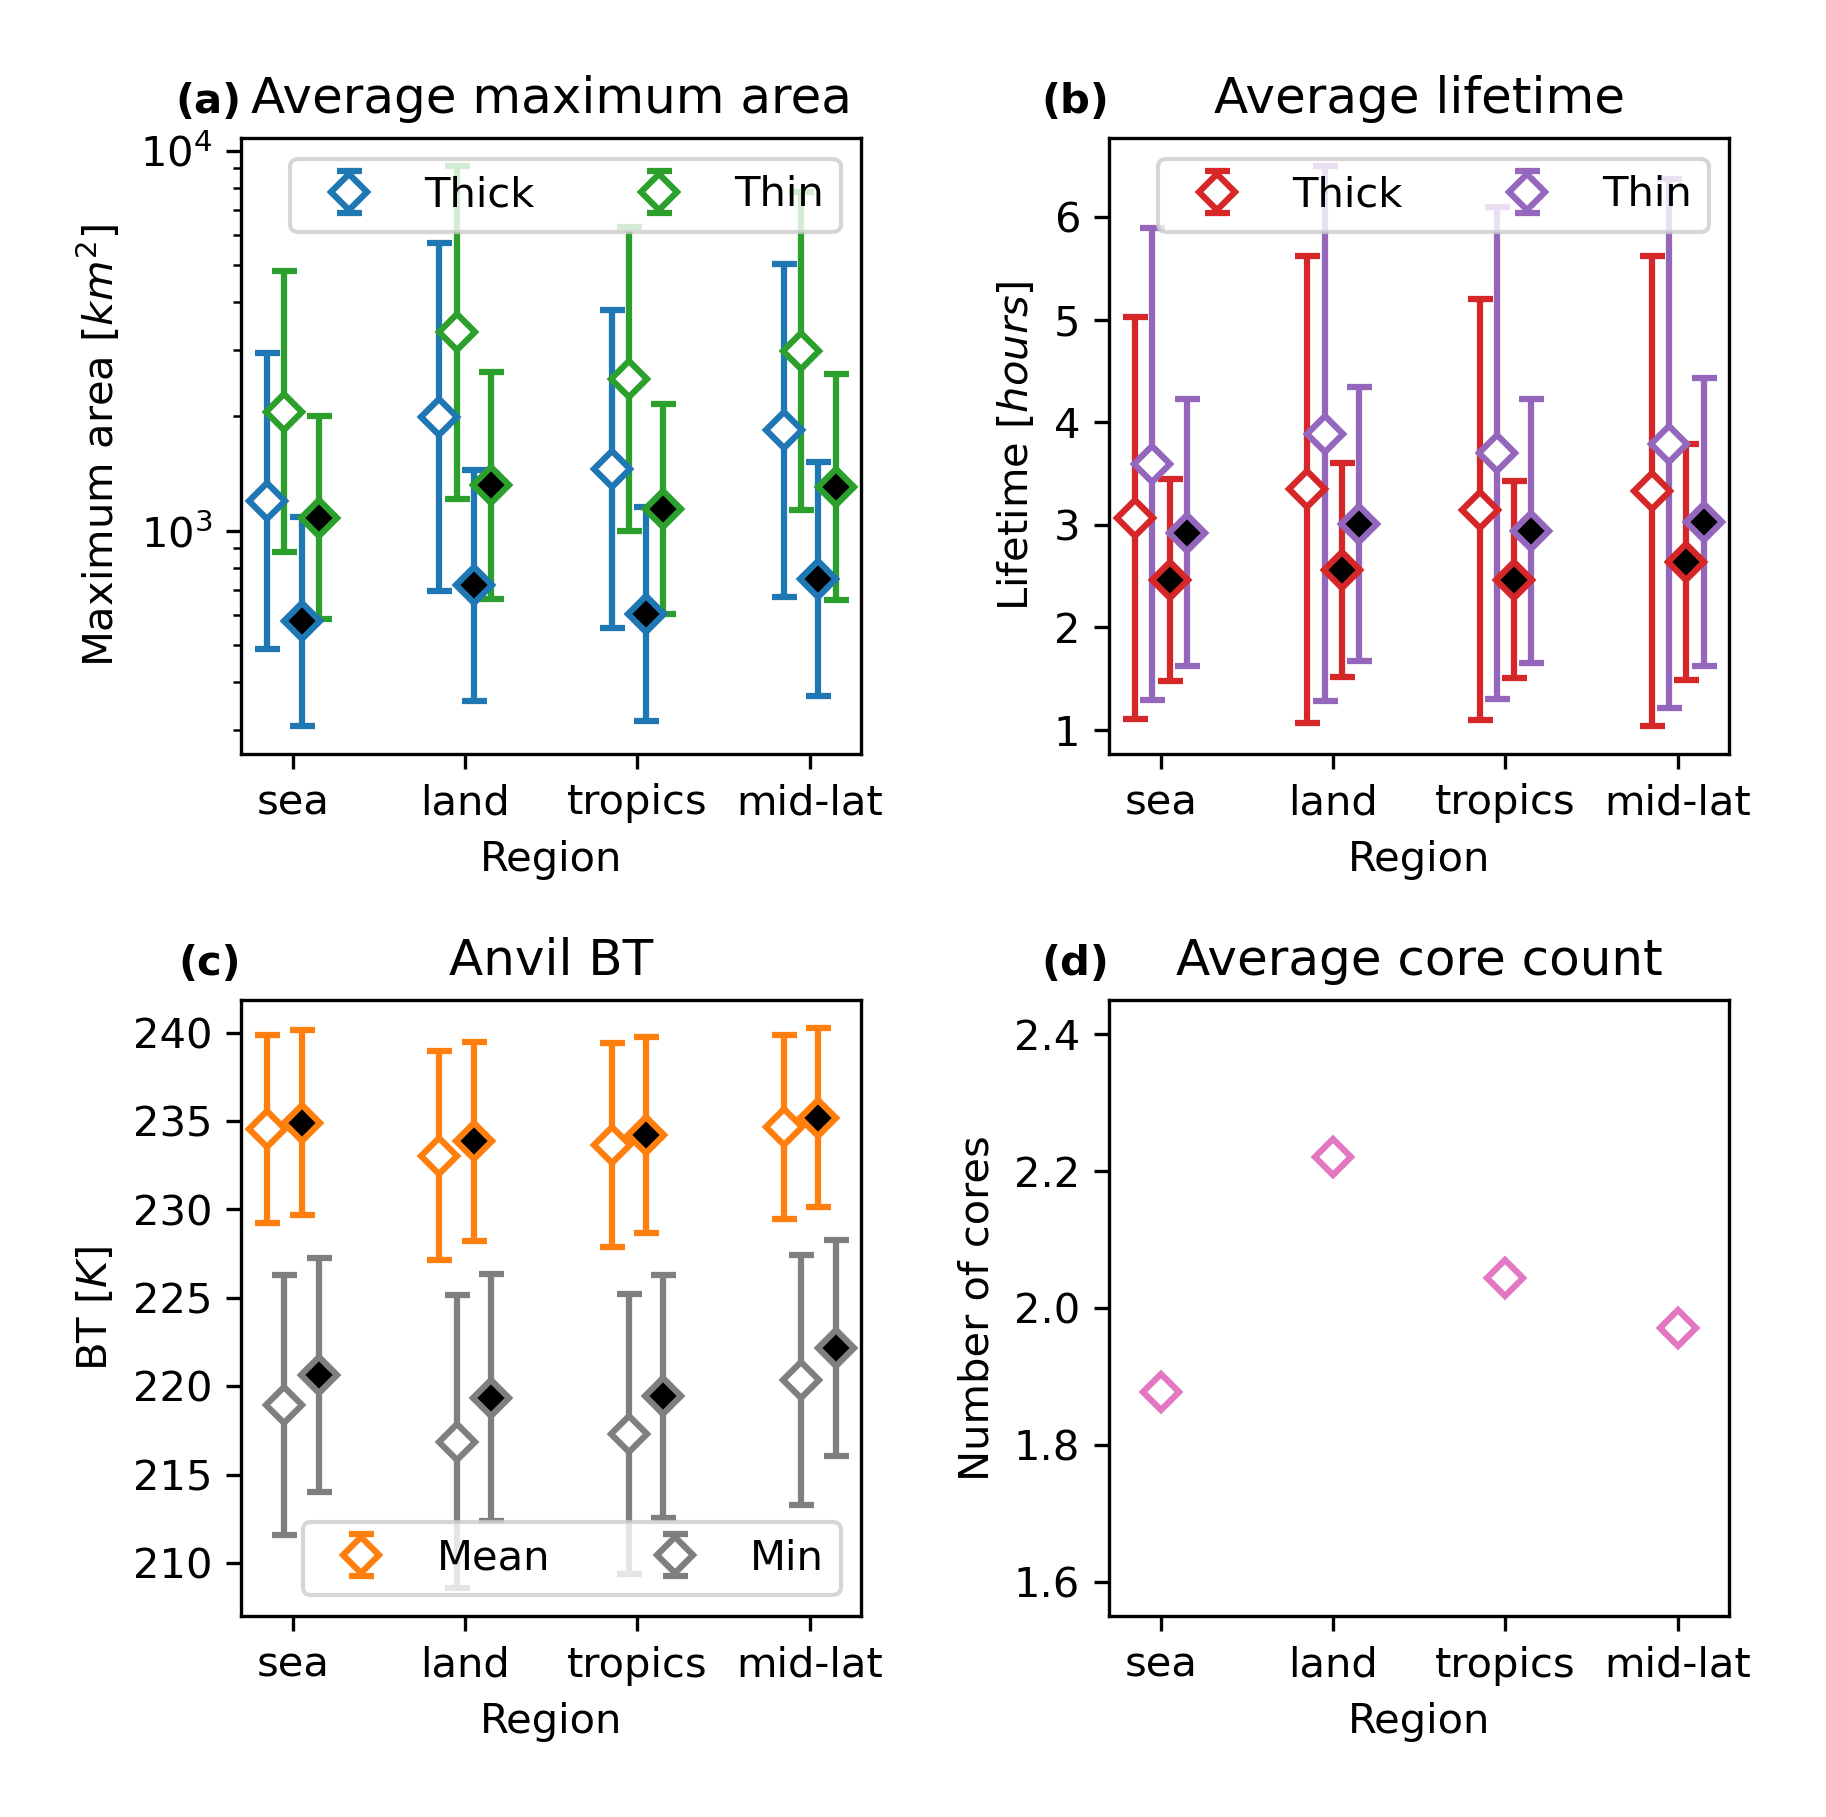
\includegraphics[width=0.9\textwidth]{figures/chapter2_22.png}
    \caption[
    The change in the average areas, lifetimes, \acrshort{bt} and number of cores of anvils observed over sea, land, tropics and mid-latitudes.
    ]{
    The change in the average (a) areas, (b) lifetimes, (c) \acrshort{bt} and (d) number of cores of anvils observed over sea, land, tropics and mid-latitudes. The points with no fill show the average across all \acrshort{dcc}s, whereas the points with the black fill show the average for isolated \acrshort{dcc}s (with one core) only. Error bars are not shown as the standard error of the mean is too small to be visible.
    }
    \label{fig:anvil_properties_regions}
\end{figure}

Figure~\ref{fig:anvil_properties_regions} shows how the averages of the maximum areas, lifetimes, \acrshort{bt} and number of cores vary between different regions.
For both isolated and multi-core convection, the average areas and lifetimes shown in fig.~\ref{fig:anvil_properties_regions}\,a and b respectively are larger over land than sea, and in the mid-latitudes than in the tropics.
For the anvil \acrshort{bt} shown in fig.~\ref{fig:anvil_properties_regions}\,c, both the mean and minimum \acrshort{bt} of anvils is colder over land than sea, and also colder in the tropics than in the mid-latitudes.
\acrshort{dcc}s over land tend to have more cores than those over the sea.

As discussed in section~\ref{sec:core_properties} regarding fig.~\ref{fig:core_region_mean_properties}, it is expected that there will be some systematic bias in these mean properties, and that this error will be covariant for land and mid-latitude, and for sea and tropics regions due to their overlap.
For both the average maximum area and the average lifetime of anvils shown in fig.~\ref{fig:anvil_properties_regions}\,a and b, evidence of this bias is seen as both land and mid-latitude regions display larger areas and longer lifetimes than sea and tropics respectively.
On the contrary, similarly to fig.~\ref{fig:core_region_mean_properties}\,d while anvils over land have colder mean and minimum \acrshort{bt} than those over the ocean, anvils in the tropics tend to be colder than those in the mid-latitudes.
This both indicates that these differences are real, and are as expected as the higher tropopause in the tropics can result in colder anvil clouds.
While a difference in the average number of cores is seen between land and ocean, little difference is seen between tropics and mid-latitudes in this regard.
The increased tendency of anvils to have multiple cores over land may influence the other differences seen in fig.~\ref{fig:anvil_properties_regions}, as more organised \acrshort{dcc}s tend to have large areas, longer lifetimes and colder \acrshort{ctt}.
However, these differences also apply to isolated \acrshort{dcc}s (those indicated by the black points in fig.~\ref{fig:anvil_properties_regions}), indicating that they are connected to changes in the convective processes and anvil evolution in the different regions rather than a sampling bias.

\subsection{Diurnal cycle of anvils}

%f
\begin{figure}[tp]
    \centering
    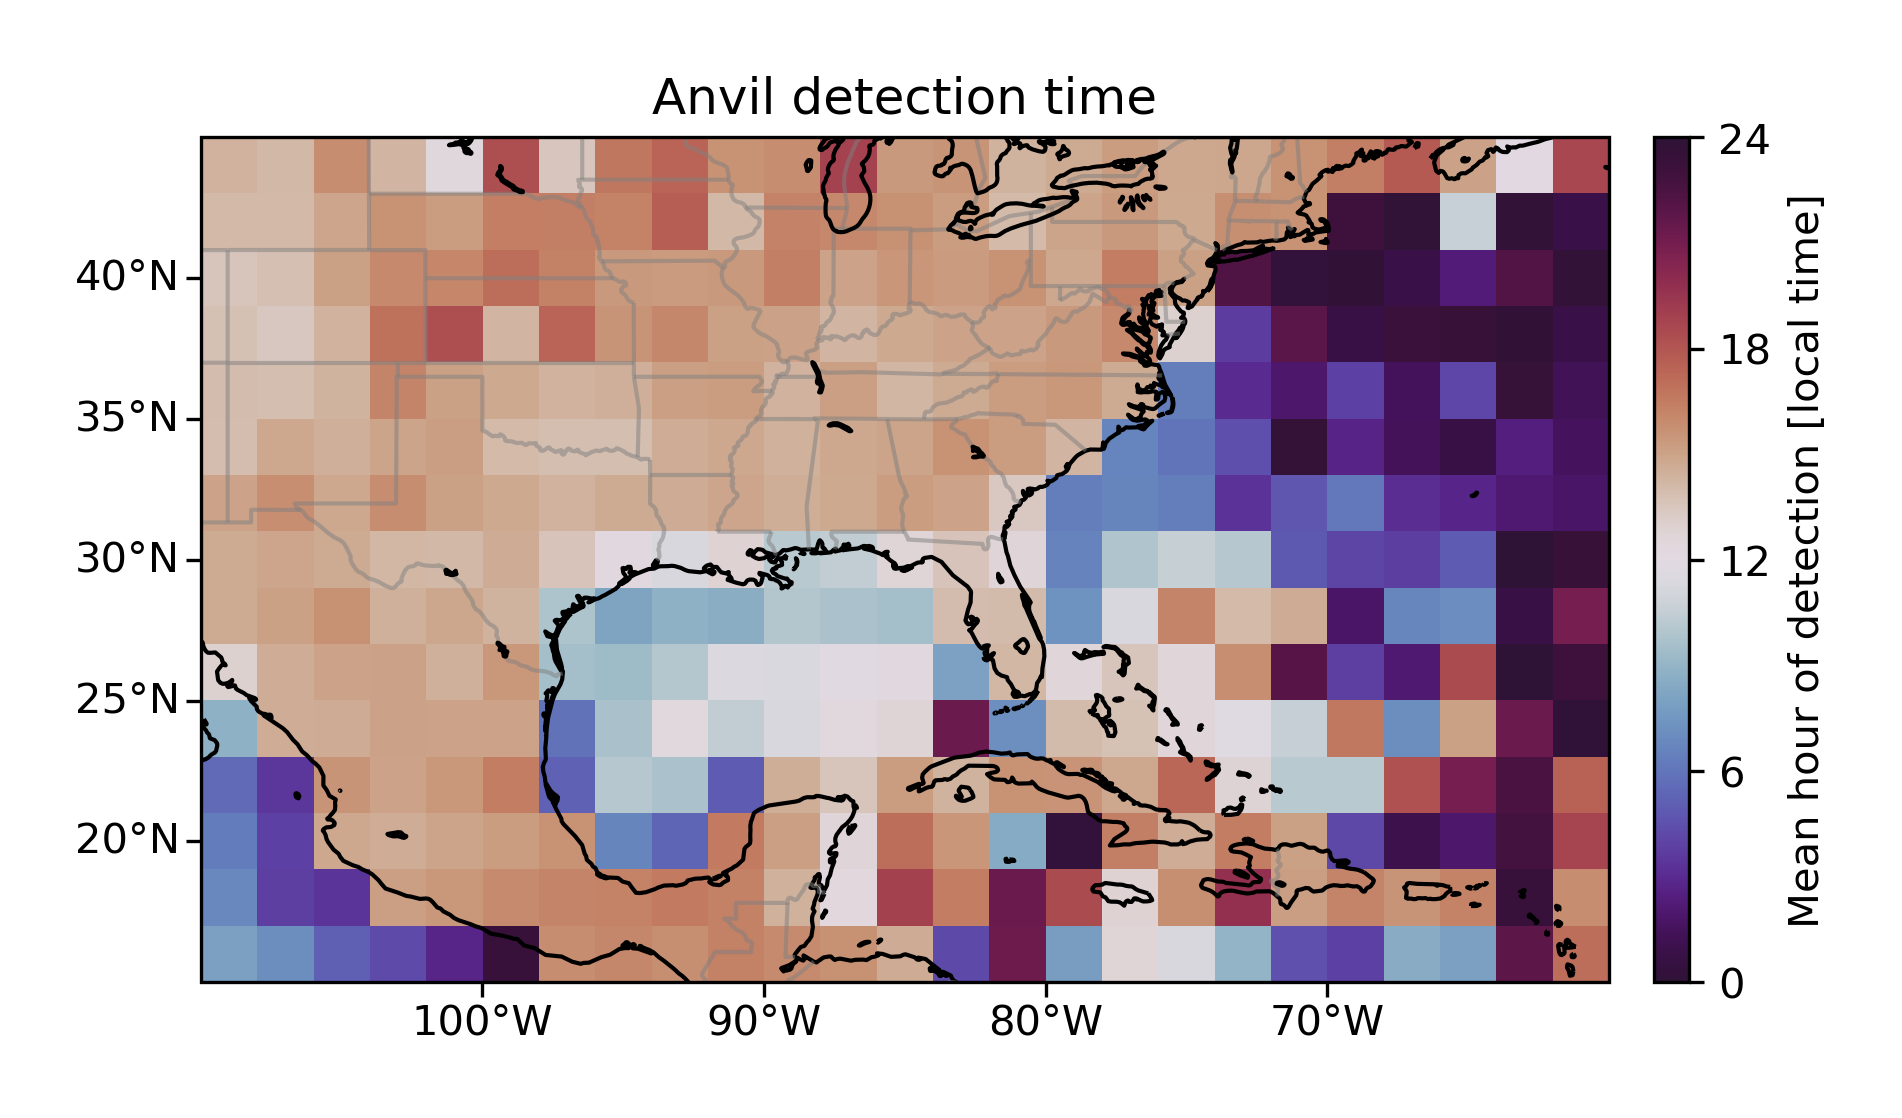
\includegraphics[width=\textwidth]{figures/chapter2_23.png}
    \caption[
    The average time of detection of anvils
    ]{
    The average time of day of detection of anvils observed within each 2\texttimes2\textdegree\ grid box, calculated as the circular mean of the local solar time.
    }
    \label{fig:anvil_detection_time_map}
\end{figure}

Figure~\ref{fig:anvil_detection_time_map} shows the average local time of day of anvil detection.
Similar to fig.~\ref{fig:core_detection_time_map} a strong land--sea contrast is seen.
However, over parts of the Caribbean Sea, the average time of anvil detection is in the afternoon rather than in the morning, which may be linked to \acrshort{dcc}s that initiate over land but have anvils which are advected over the ocean.
There is also a later average time of detection of anvils over the \acrshort{ngp} region, although this shows less of a contrast with surrounding land regions than that of the core initiation times.
This indicates that the second peak of core convective activity during the nighttime and early morning in fig.~\ref{fig:core_ngp_contrast} is linked to long-lived, multiple core systems including \acrshort{mcs}s, similar to what was found by \citet{feng_spatiotemporal_2019}.

%f
\begin{figure}[tp]
    \centering
    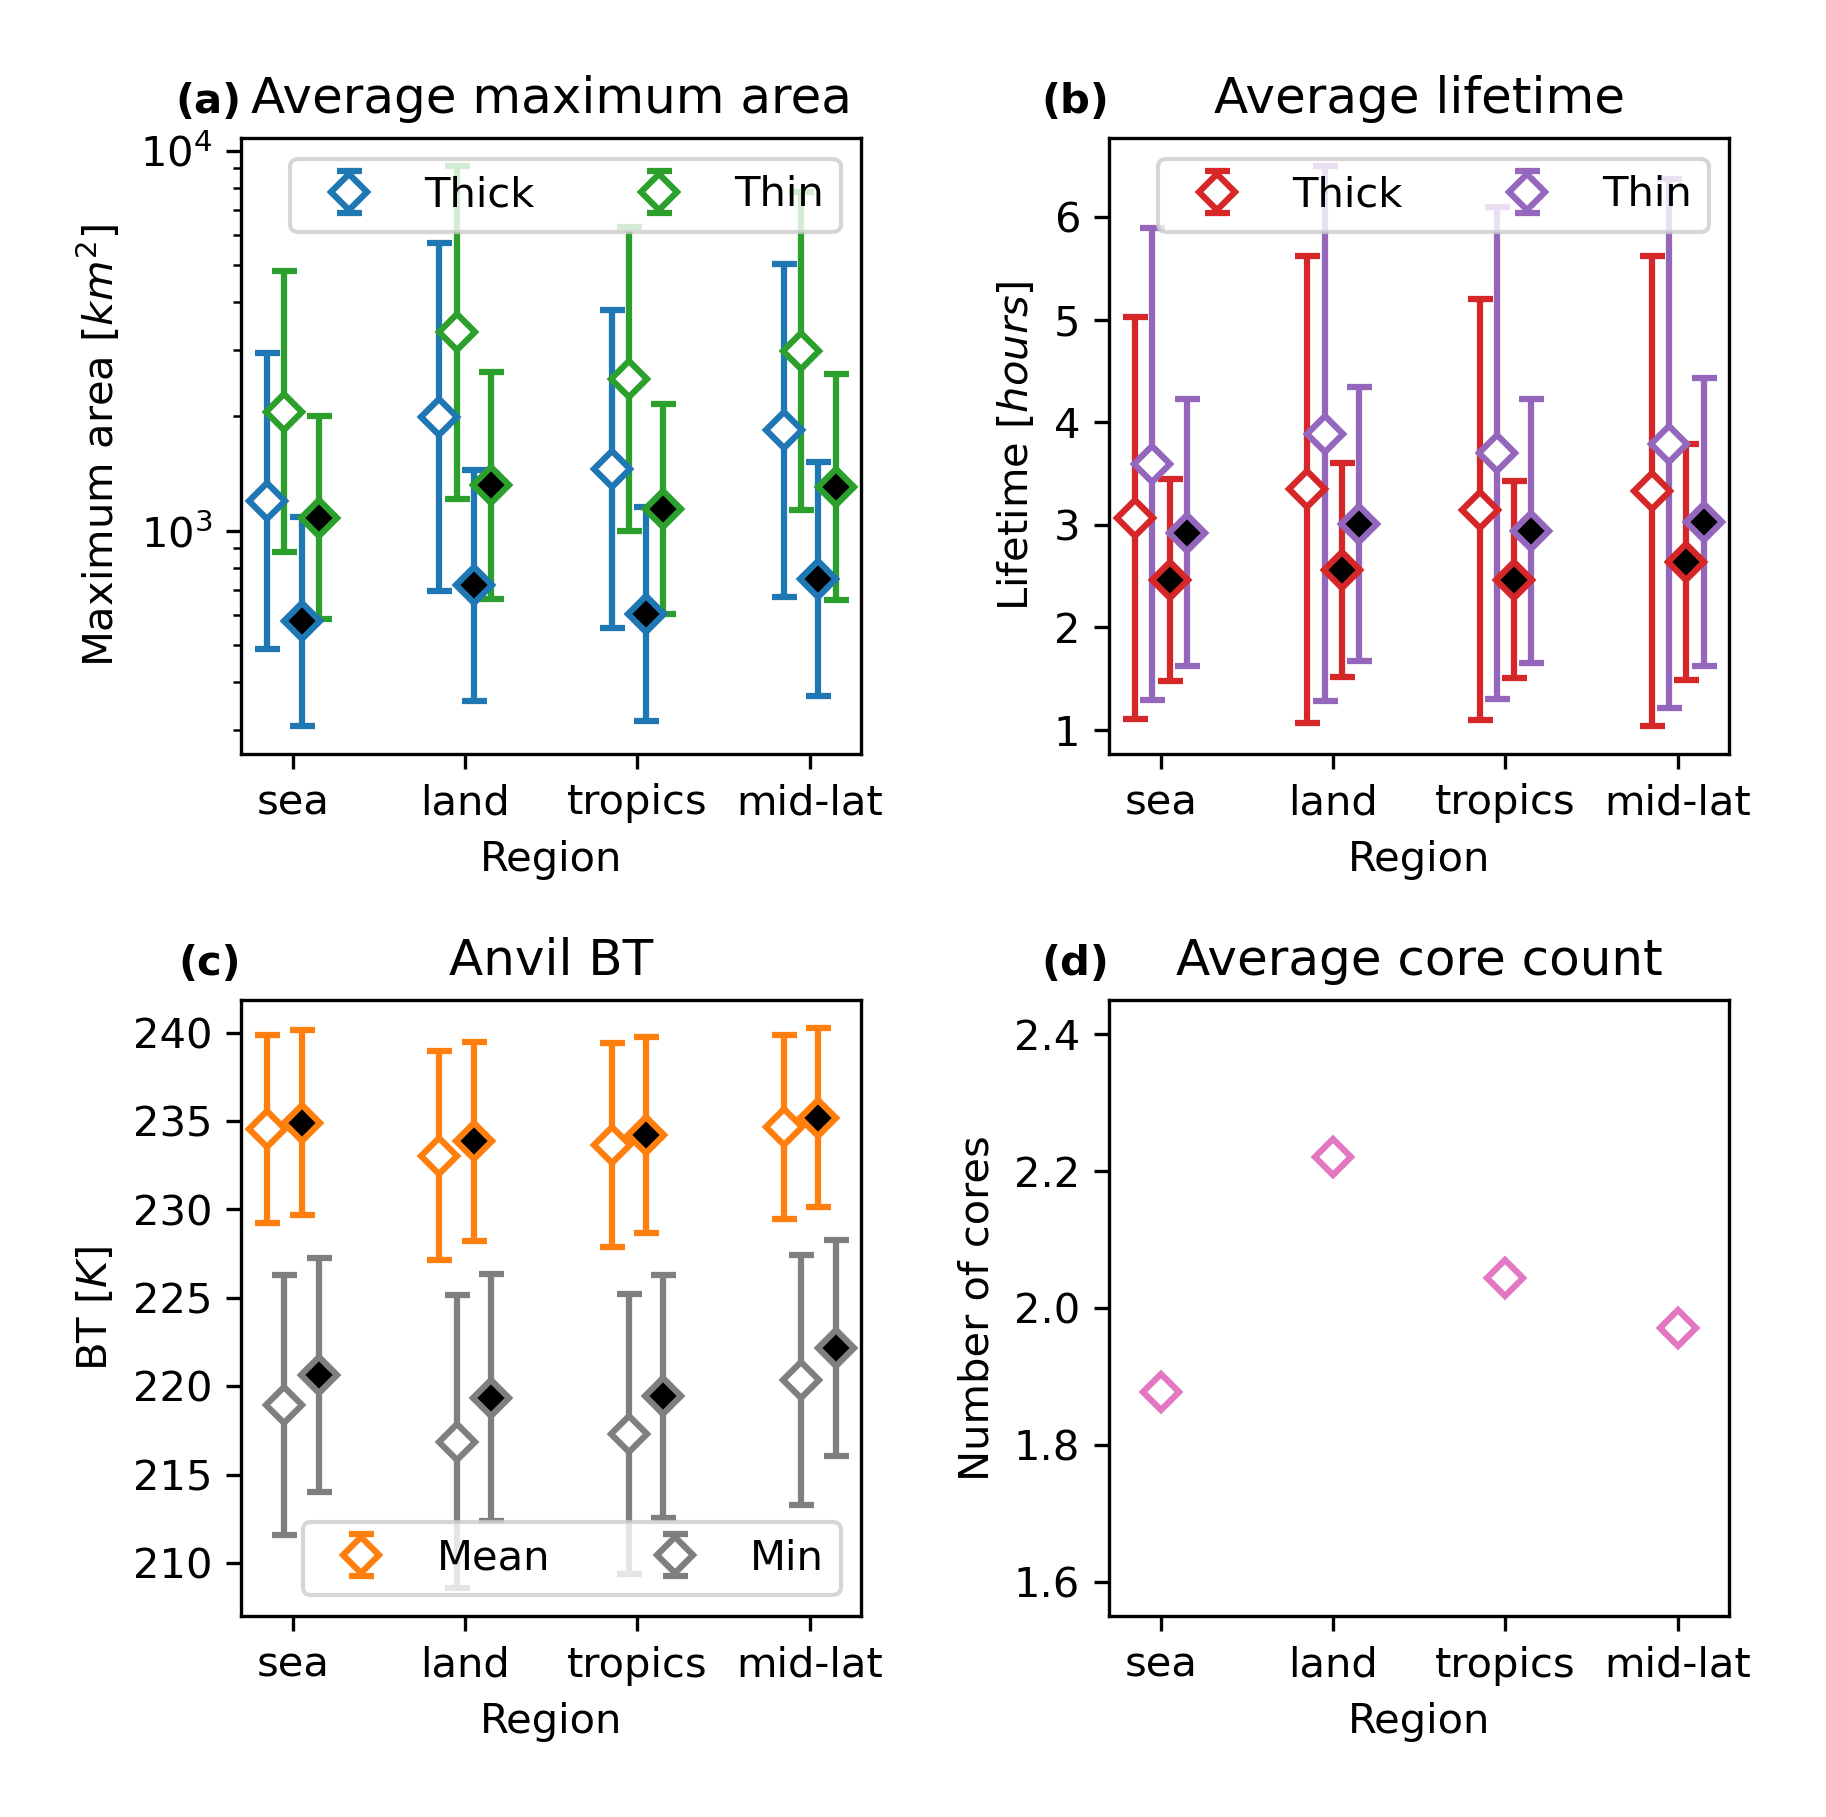
\includegraphics[width=\textwidth]{figures/chapter2_24.png}
    \caption[
    The diurnal distributions of the local time of detection for anvils detected over sea, land, tropics and mid-latitudes
    ]{
    The diurnal distributions of the local time of detection for anvils, binned by hour detected over (a) sea, (b) land, (c) tropics (\textless 30\,\textdegree N) and (d) mid-latitudes (\textgreater 30\,\textdegree N). The hatched area shows the proportion of each distribution associated with multi-core anvils.
    }
    \label{fig:anvil_diurnal_distributions}
\end{figure}

In fig.~\ref{fig:anvil_diurnal_distributions} the diurnal cycles of anvil detections are plotted by region.
The distributions generally match those seen of the core detection times shown in fig.~\ref{fig:core_diurnal_land_sea}, as the majority of the observed anvils are isolated systems.
The diurnal cycle of anvil detections over the sea is much less pronounced however, which may lead to the increased variability seen in fig.~\ref{fig:anvil_detection_time_map}.
When comparing the hatched areas, indicating the proportion of the distribution consisting of multi-core anvils, over land, tropics and mid-latitudes the initiation of these organised systems occurs earlier in the day compared to isolated \acrshort{dcc}s.

%f
\begin{figure}[tp]
    \centering
    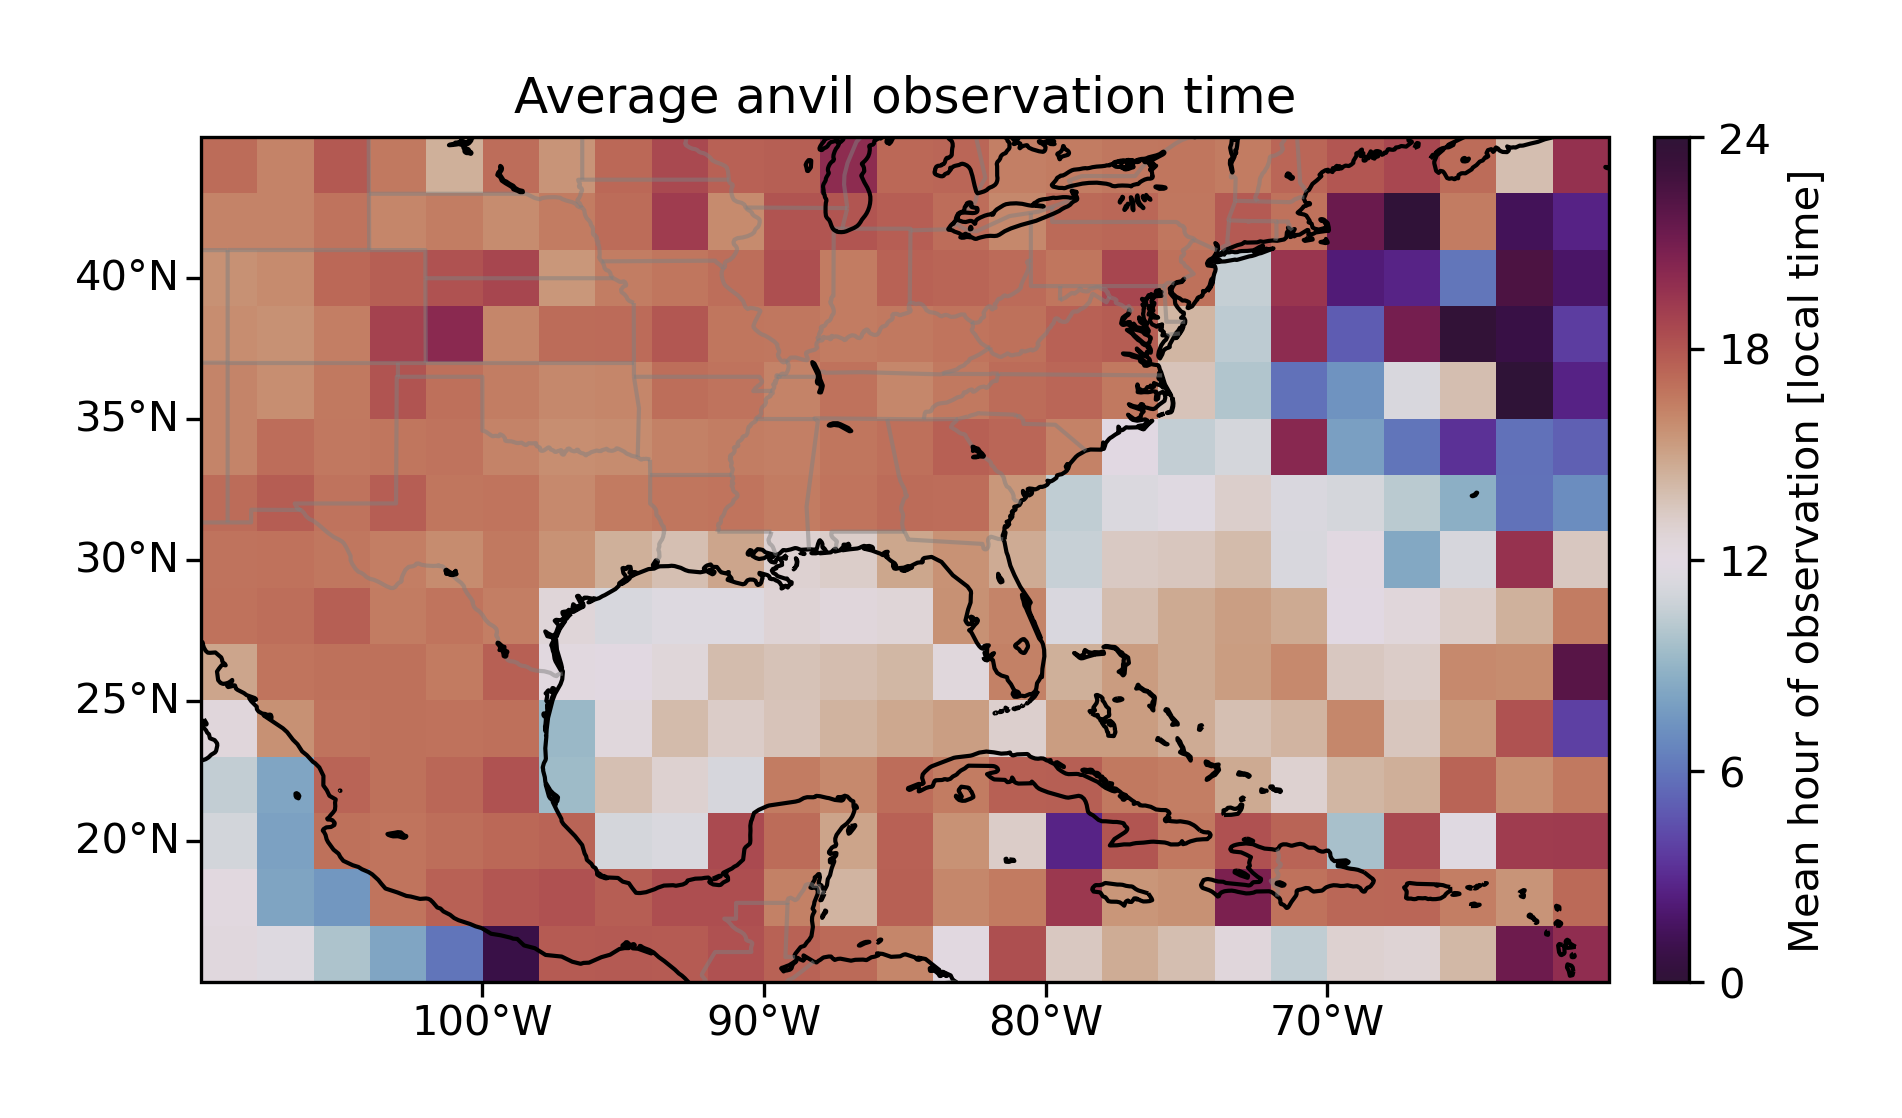
\includegraphics[width=\textwidth]{figures/chapter2_25.png}
    \caption[
    A map showing the average time of observation of anvils
    ]{
    The average time of day of observation of anvils observed within each 2\texttimes2\textdegree\ grid box, calculated as the circular mean of the local solar time. Unlike fig.~\ref{fig:anvil_detection_time_map}, this is the average of the time of observation at every time step along the anvil lifetime.
    }
    \label{fig:anvil_observation_time_map}
\end{figure}

Figure~\ref{fig:anvil_observation_time_map} shows the average time of observation for anvils.
Unlike the previous map of detection time shown in fig.~\ref{fig:anvil_detection_time_map}, in this figure the average of all the time steps at which an anvil is detected is shown.
Over the land, the effect is to shift the timing of the maximum to a later point in the diurnal cycle, which is a shift of approximately half the average anvil lifetime.
Over sea, however, there is a much larger shift with much of the Caribbean showing a similar time of day to adjacent land regions.

%f
\begin{figure}[tp]
    \centering
    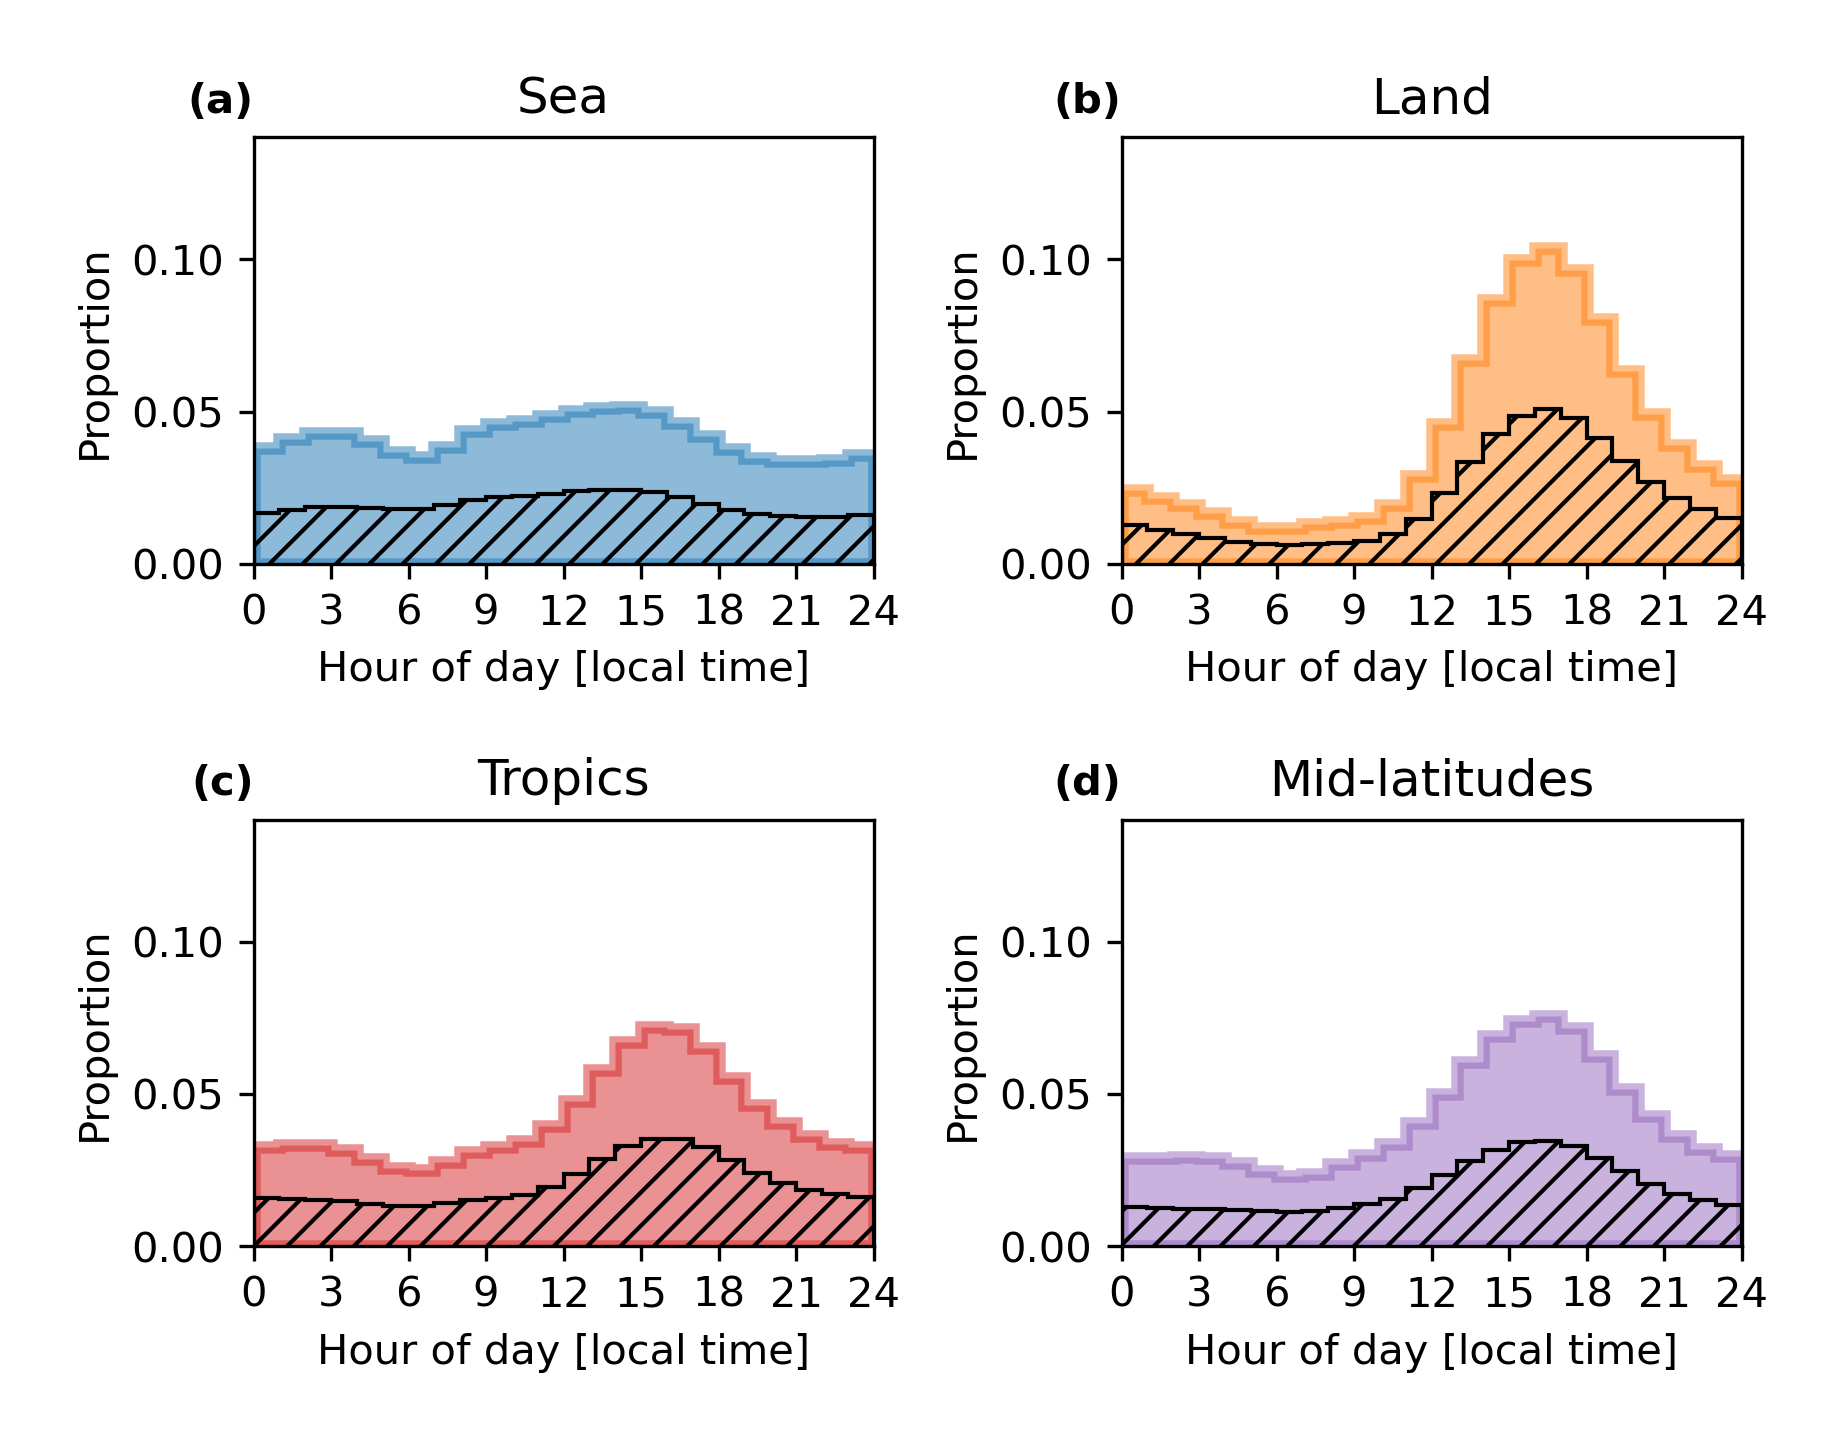
\includegraphics[width=\textwidth]{figures/chapter2_26.png}
    \caption[
    The diurnal distributions of the local time of observation for anvils detected over sea, land, tropics and mid-latitudes
    ]{
    The diurnal distributions of the local time of observation for anvils, binned by hour detected over (a) sea, (b) land, (c) tropics (\textless 30\,\textdegree N) and (d) mid-latitudes (\textgreater 30\,\textdegree N). The hatched area shows the proportion of each distribution associated with multi-core anvils.
    }
    \label{fig:anvil_diurnal_obs_distributions}
\end{figure}

Figure~\ref{fig:anvil_diurnal_obs_distributions} shows the diurnal cycle of anvil observations for each of the four regions.
For the land, tropics and mid-latitudes regions, there is a shift in the peak of the distribution to 4--5\,pm, along with a lengthening of the right tail of the distribution.
The distribution of multi-core anvils appears to match that for all \acrshort{dcc}s.
While in fig.~\ref{fig:anvil_diurnal_distributions} the initiation time of these organised anvils tended to be earlier in the day, their longer lifetime means that they tend to exist, on average, at the same times.
However, this longer lifetime also means that organised \acrshort{dcc}s make up a larger proportion of anvil observations during the nighttime and morning, and fewer during the afternoon during the peak in isolated \acrshort{dcc}s.
In fig.~\ref{fig:anvil_diurnal_obs_distributions}\,a, the peak of the diurnal distribution over the sea is in the afternoon, with a gradual increase of observations throughout the day.
Previous research has shown that solar heating during the daytime increases the area and lifetime of anvils \citep{gasparini_diurnal_2022}, which may explain why there are more anvils observed during the day, despite more initiations occurring at night.

%f
\begin{figure}[tp]
    \centering
    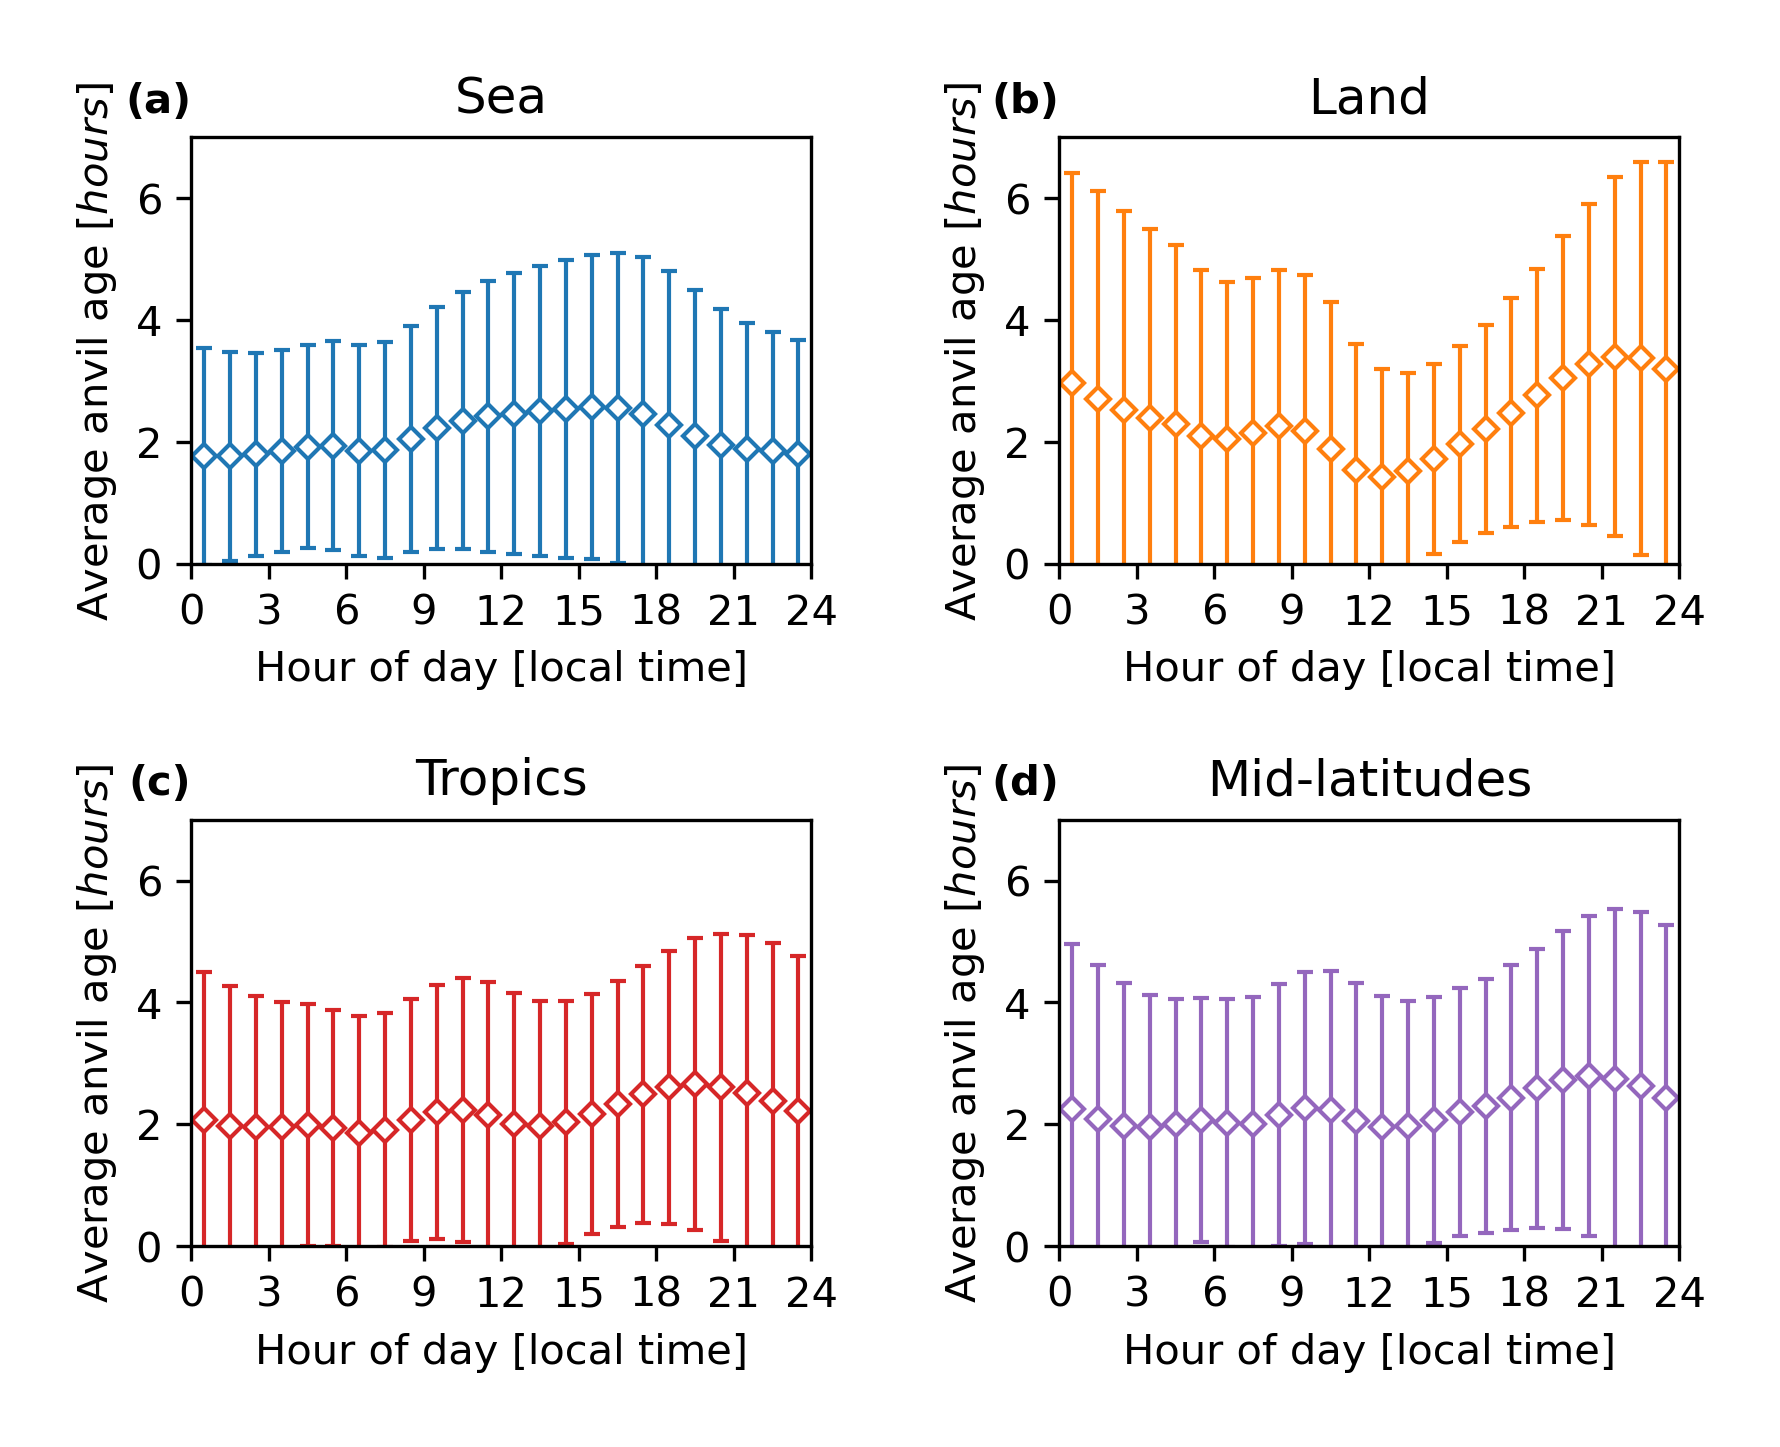
\includegraphics[width=\textwidth]{figures/chapter2_27.png}
    \caption[
    The average age of anvils observed over sea, land, tropics and mid-latitudes throughout the diurnal cycle.
    ]{
    The average age of anvils observed over (a) sea, (b) land, (c) tropics (\textless 30\,\textdegree N) and (d) mid-latitudes (\textgreater 30\,\textdegree N) throughout the diurnal cycle. Error bars are not shown as the standard error of the mean is too small to be visible.
    }
    \label{fig:anvil_diurnal_age}
\end{figure}

The difference in the distributions of anvil initiation times and anvil observation times indicates that the lifetime and age of observed anvils change across the diurnal cycle.
Figure~\ref{fig:anvil_diurnal_age} shows the average age of anvils observed during each hour of the diurnal cycle.
The increase in the age of anvils observed over sea throughout the daytime provides further evidence for the enhancement of anvil lifetime by \acrshort{sw} radiation.
For anvil observations over land, there is greater interaction with the diurnal cycle of convection.
In fig.~\ref{fig:anvil_diurnal_age}\,b there is a minima of the anvil age between midday and 1\,pm, coinciding with the onset of the afternoon peak of anvil initiations seen in fig.~\ref{fig:anvil_diurnal_distributions}\,b.
The age then increases to a maximum at around 10\,pm, before decreasing again until midday.
The variation in the average age of observed anvils is larger over land than over the ocean.
Over the tropics and mid-latitudes however, the combination of opposite signals from sea and land means that there is much less variation of anvil age across either region.


\section{Summary}  %% \conclusions[modified heading if necessary]

By applying the \textit{tobac-flow} algorithm to five years of multi-channel \acrshort{bt} observations from the \acrshort{goes}-16 \acrshort{abi} \acrshort{conus} scan region, an extensive dataset of \acrshort{dcc} cores and anvils has been produced, including their properties over time.
Containing approximately 1.6 million cores and 400 thousand anvils which are considered valid for analysis over their entire lifecycle, this dataset provides valuable information about their properties, distributions and lifecycle in a Lagrangian framework.
With five-minute temporal resolution, the properties of developing convective cores can be measured accurately, and then linked to the subsequent evolution of the anvil cloud.

Several key differences in the seasonal, diurnal and regional patterns are seen for \acrshort{dcc}s across North America.
The spatial distribution of \acrshort{dcc} cores depends strongly on the seasonal cycle.
There is a large land/sea contrast in the time of initiation, which also displays a sea breeze effect which extends for approximately 200\,\unit{km} inland.
The properties of cores themselves, including the lifetime, cooling rate, and time of initiation, have regional dependencies, with more intense convection occurring over land during the daytime and in the tropics.

These differences extend to the anvils produced by these convective cores.
The seasonal and diurnal cycles of anvils are closely related to those of the convective cores.
Furthermore, there are differences in the properties of anvils between different regions corresponding to differences in convective properties.
In particular, \acrshort{dcc}s over land have larger areas, longer lifetimes and colder \acrshort{bt} than those over the ocean.

While the majority of observed anvil clouds are associated with a single growing core, there are also a large number of multi-core anvils detected in our dataset.
The frequency of multi-core anvils as a proportion of all observed anvils increases with latitude.
Finally, while the properties of the individual growing cores observed in single- and multi-core anvils show no significant difference, the lifetime and area of anvils show a large increase with the number of cores.

Some of these findings, such as the larger area of \acrshort{dcc}s over land, contrast with studies made using polar-orbiting satellites \citep{ge_contrasting_2024}.
However, our investigation of the age of anvils observed throughout the diurnal cycle provides a mechanism for this discrepancy.
The area of \acrshort{dcc} anvils evolves as they age \citep{futyan_deep_2007}.
Impacts of radiative heating and the diurnal cycle act to modify this however \citep{gasparini_diurnal_2022}.
As a result, the average age of observed anvils varies throughout the day.
At the time of the Cloudsat overpass (1:30\,pm), the average age of anvils over land is at its minima, while those over the ocean are near their maxima.
As a result, the average area of anvils observed at this time over land would be smaller than those over the ocean, not because of a difference in their processes but because they are being observed earlier in their lifetime before they have reached their maximum area.
While at the nighttime overpass time (1:30\,am) the average age of anvils over land is older, the reduced number of land \acrshort{dcc}s at this time means that any set of snapshot observations will be biased towards younger anvils over land.

By using temporally resolved observations, and placing these in a Lagrangian framework using cloud tracking, these changes in convective cloud behaviour can be accounted for across the diurnal cycle.
Furthermore, linking the properties of the developing cores to the resulting anvil clouds over their entire lifetime provides the potential to investigate how the processes of the former affect the latter.
Connecting these properties allows investigation of previously uncertain \acrshort{dcc} processes, and, in particular, may help shed light on how anvil optical properties, structure and diurnal cycle respond to climate change.

\chapter{Contrasting effects of convective intensity and organisation on the structure and lifecycle of \acrshort{dcc}s} \label{chp:anvil_structure}

\section{Introduction}

Understanding how the structure of anvil clouds changes in response to changes in convective behaviour is vital to understanding the radiative impacts and climate feedbacks of \acrshort{dcc}s.
Around 50\% of cirrus clouds in the tropics originate from deep convection \citep{massie_distribution_2002, luo_characterizing_2004}.
Overall, anvil clouds have a near-neutral radiative impact on the tropics, despite their large \acrshort{sw} reflectance and \acrshort{lw} absorption \citep{hartmann_effect_1992, hartmann_tropical_2016}.
Their radiative effect is not homogeneous however; while the optically thick portion of anvil clouds generally have a cooling effect at the \acrshort{toa}, the thin, detrained cirrus has a strong warming effect \citep{berry_cloud_2014}.
As a result, changes in convective activity that result in a change in the size and structure of anvil clouds may have large impacts on the climate.

The change of anvil cloud area in response to warming---the iris effect \citep{lindzen_does_2001, bony_thermodynamic_2016}---is generally considered to have a cooling feedback in response to climate change.
However, it is the largest source of uncertainty in cloud--climate feedbacks, with around a third of models predicting a warming response \citep{sherwood_assessment_2020}.
To address this uncertainty, a better understanding of the links between convective processes and anvil properties, changes in anvil structure and the properties of ice clouds are required \citep{gasparini_opinion_2023}.

Assessing the extent of thin anvil cirrus is challenging due to the difficulties in observing these clouds using \acrshort{ir} radiometers.
The low emissivity of thin cirrus clouds means that observed \acrshort{bt} is dominated by radiances from the lower atmosphere and surface below.
\citet{protopapadaki_upper_2017} used cloud emissivity and cloud top pressure, rather than \acrshort{bt}, to detect convective cores, thick and thin anvil cirrus clouds.
Data from the AIRS instrument was used to retrieve these emissivity values, as the hyperspectral sounder is more sensitive to thin cirrus than \acrshort{ir} radiometers.
They then compared the proportion of each anvil cloud consisting of thin anvil to the minimum observed cloud top temperature within the convective core, a proxy for the convective depth which is, in turn, a proxy for convective intensity.
It was found that the thin cirrus anvil proportion increased with colder cloud top temperatures, indicating that stronger convection increases the detrainment of thin cirrus.

\citet{takahashi_relationships_2017} built upon this study using collocated measurements from the \acrfull{cpr} aboard CloudSat.
The \acrshort{cpr} measurements provide the echo top height, measuring the convective depth directly, and also provide another proxy for convective intensity, the echo top distance, which is independent of convective depth \citep{takahashi_characterizing_2014}.
It was again found that the proportion of thin cirrus increased with the echo top height, and also increased with decreasing echo top distance (indicating stronger convection).

It should be noted that both of these studies were performed using observations from polar-orbiting satellites in the A-train, and so do not fully sample the diurnal cycle.
While both studies consider the maturity of the \acrshort{dcc}s observed, the thin anvil proportion is measured at a single point in time, and so differences in the lifetime of the thick and thin anvil cirrus are not considered.
It is expected that the structure of an anvil will change over its lifetime, with the thin anvil fraction increasing as the anvil dissipates.
However, the observed \acrshort{bt} of the anvil also changes over its lifetime \citep{futyan_deep_2007}, and so the use of \acrshort{bt} as a proxy for convective intensity is not an independent measurement.
While the use of echo top height avoids this confounding issue, these collocated measurements can only be made when the \acrfull{dcc} is convectively active and so cannot be used to assess the structure of dissipating anvils.

Chapter~\ref{chp:lifecycle} presented a large dataset of tracked \acrshort{dcc}s, including growing cores, and thick and thin anvils, and showed that this dataset captures relations between convective processes and anvil properties.
Using geostationary satellite observations, changes in the structure of \acrshort{dcc} anvils can be investigated throughout their lifecycles, along with changes in the lifetime of both thick and thin anvils.
Furthermore, the impacts of convective organisation on anvil structure can be investigated by taking into account the number of cores associated with each anvil.


\section{Data}

The dataset of tracked \acrshort{dcc}s first presented in chapter~\ref{chp:lifecycle} is utilised here to investigate how the structure of observed \acrshort{dcc}s depends on the properties of their convective cores.
Produced using the method detailed in chapter~\ref{chp:tracking_method}, convective cores are tracked during their vertically growing period, and thick and thin anvils are subsequently tracked using two different channel combinations.
Changes in the proportion of thick and thin anvil coverage, considering both spatial extent and the lifecycle of the anvil cloud, can be investigated.

Data filtering is applied to detected anvils according to the criteria shown previously in table~\ref{table:anvil_validity_criteria}.
This results in a total of 391,050 anvils considered for analysis, which between them are connected to a total of 792,522 cores.
The filtering requires that every anvil in the analysis dataset begins with a valid observed core, ensuring that the subsequent development of the anvil can be linked to the properties of the core.
In addition, it ensures that each anvil is observed for its entire lifetime, and the entire extent of both thick and thin anvil are observed over this period.
While this does mean that fewer large anvils are considered valid as their greater extent means that they are more likely to intersect the edges of the domain, it ensures that changes in both thick and thin anvil areas can be considered robust over the entire lifecycle of the analyses anvils.

The dataset contains a range of properties relating to the observed \acrshort{dcc}s.
This chapter will focus on how the area of the detected cores, thick and thin anvils change with each time step.
Two related properties are also analysed; the maximum area of the thick and thin anvil, i.e.\ the area at the time step when the anvil reaches its maximum observed extent, and the total area which is the sum of the areas observed at each time step over each anvils lifetime.
The thin anvil proportion refers to the area of the detected thin anvil divided by the total area of both anvil and core.
In general, this is calculated as the total over the entire \acrshort{dcc} lifetime, although section~\ref{sec:composite_results} will investigate how this changes over the \acrshort{dcc} lifecycle.

There is additional consideration on how the \acrshort{bt} of each core and anvil change over time.
The area-weighted average of the 10.4\,\unit{\mu m} \acrshort{bt} is taken at each time step for each core, thick and thin anvil.
The 10.4\,\unit{\mu m} \acrshort{lw} window \acrshort{bt} has a minimal contribution from water in the atmosphere, and so can provide temperature measurements of clouds from near the surface to the top of the atmosphere.
It should be noted that the observed \acrshort{bt} is affected by the emissivity of the cloud, and so for thin cirrus it will be warmer than the \acrshort{ctt} due to the contribution from the atmosphere below.
As a result, the mean \acrshort{bt} of the thick anvil is used as a proxy for convective cloud height as this avoids a bias from the warmer thin anvil.
The (negative) cooling rate of each core is calculated as the largest change in the mean core \acrshort{bt} measured over any 15-minute period.
This relates to the vertical growth of the \acrshort{dcc} core as discussed in section~\ref{sec:theory_core}, with a cooling rate of 1\,K$\cdot\mathrm{minute^{-1}}$ corresponding to a vertical growth rate at the cloud top of 2.5\,$\mathrm{ms^{-1}}$.

\section{Method}

\subsection{Detection of thick and thin anvils}

Observing thin cirrus anvils using satellite \acrshort{bt} is difficult due to their low emissivity.
Furthermore, \acrshort{bt} is affected both by the height of the observed cloud and its optical thickness.
As shown in fig.~\ref{fig:optical_depth_channels}, the observed \acrshort{bt} increases as optical depth decreases.
For detection using a fixed threshold, as used in many anvil detection algorithms, this means that the limit of optical depth at which the anvil is detected increases as the height of the cloud decreases.
This results in the detected anvil area varying with height, with an anvil at a lower altitude being detected as smaller than one at a higher altitude even if their size and structure are otherwise identical.
This problem with detected anvil area using \acrshort{bt} thresholds was identified as early as \citet{augustine_mesoscale_1988}, but remains a feature of many detection algorithms to this day (see e.g.\ section~\ref{sec:tracking_timeline}).

%f
\begin{figure}[tp]
    \centering
    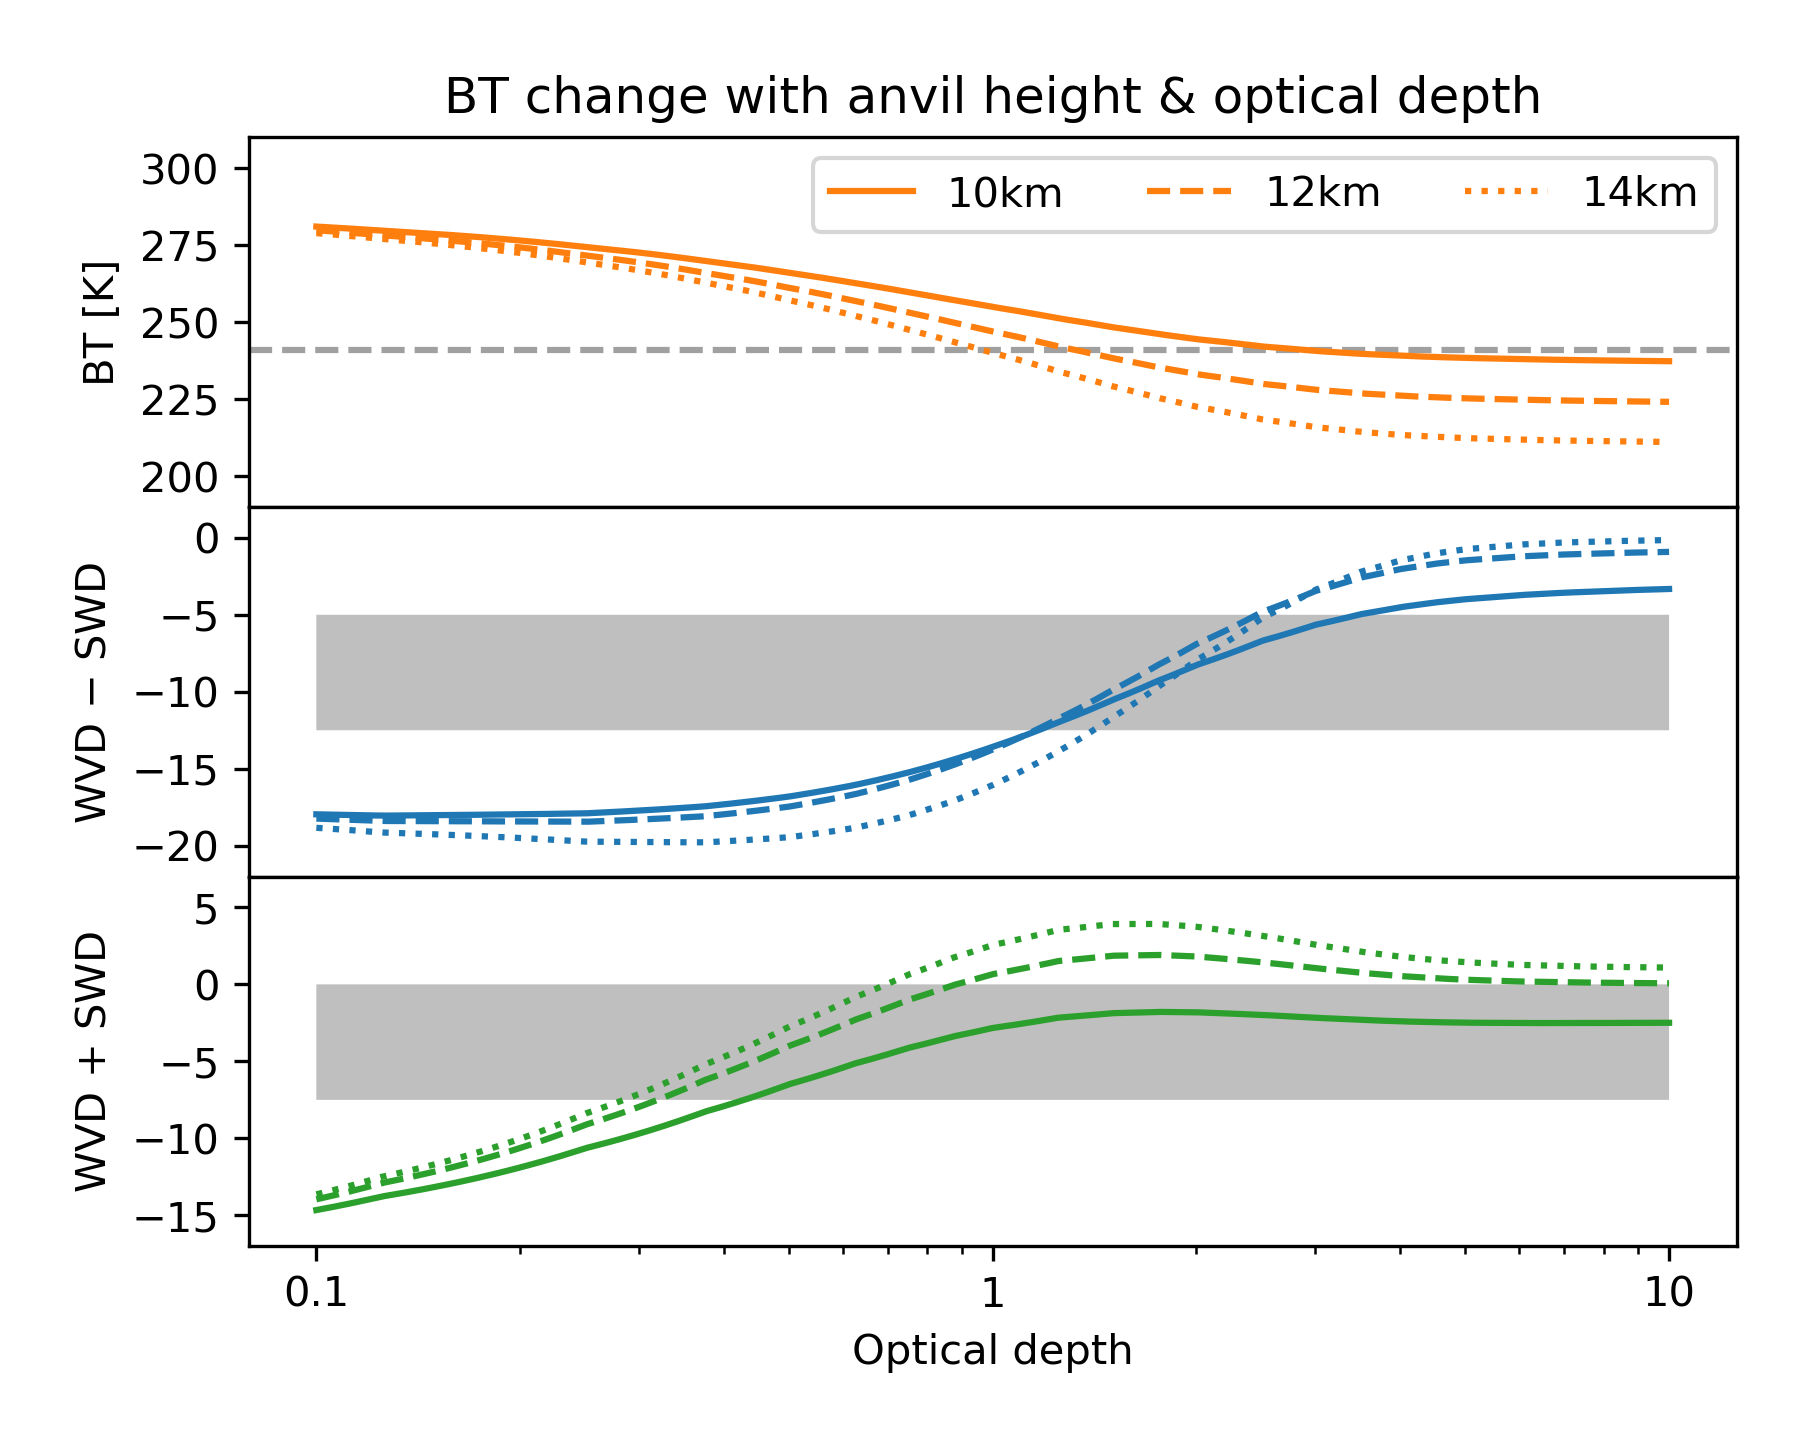
\includegraphics[width=0.9\textwidth]{figures/chapter3_01.png}
    \caption[
    Simulated \acrshort{abi} \acrshort{bt} observations of \acrshort{dcc} anvils at a range of heights and optical depths for detection of thick and thin anvil detection
    ]{
    Simulated \acrshort{abi} \acrshort{bt} observations for \acrshort{dcc} anvils at 10\,\unit{km} (solid lines), 12\,\unit{km} (dashed lines) and 14\,\unit{km} (dotted lines) at optical depths between 0.1 and 10. Panels show (top) 10.4\,\unit{\mu m} \acrshort{bt}; (middle) \acrshort{wvd} minus \acrshort{swd}, used in thick anvil detection; and (bottom) \acrshort{wvd} plus \acrshort{swd}, used in thin anvil detection. The grey dashed line shows the 241\,\unit[K] threshold, and the grey shaded regions show the range in which cloud edge detection is performed for thick and thin anvils.
    }
    \label{fig:bt_wvd_swd_height_od}
\end{figure}

While observing the thin cirrus anvil is challenging, section~\ref{sec:anvil_detection} showed that thin anvil cirrus can be detected using a combination of the \acrshort{wvd} and \acrshort{swd} differences from \acrshort{abi}.
Furthermore, the use of channel differences reduces the height dependence of the detection of anvils compared to the use of a single \acrshort{bt}.
Figure~\ref{fig:bt_wvd_swd_height_od} shows simulated \acrshort{bt} observations using the libRadTran model \citep{emde_libradtran_2016}, as described in section~\ref{sec:detection_theory}.
The top panel shows simulation \acrshort{bt} observations by \acrshort{abi} at 10.4\,\unit{\mu m} at heights of 10, 12 and 14\,\unit{km} (shown by the solid, dashed and dotted lines respectively).
Also shown by the grey, dashed line is an example of the 241\,\unit{K} \acrshort{bt} threshold.
At this threshold there is substantial variance in the limit of \acrshort{od} at which anvil clouds are detected, which ranges from 1 at 14\,\unit{km} to 3 at \unit{km}.
This provides clear support for the argument made by \citet{augustine_mesoscale_1988} that the anvil area detected using this threshold is ``subjective''.

The middle and bottom panels in fig.~\ref{fig:bt_wvd_swd_height_od} show the simulated \acrshort{bt} for the combinations of \acrshort{wvd} minus \acrshort{swd} and \acrshort{wvd} plus \acrshort{swd} respectively across a range of \acrshort{od}.
Section~\ref{sec:anvil_detection} describes how these two channel combinations are used for the detection of thick and thin anvils.
In both panels, the grey shaded region shows the \acrshort{bt} range in which edge detection is used to find the anvil area.
Compared to 10.4\,\unit{\mu m} \acrshort{bt}, the \acrshort{wvd} minus \acrshort{swd} combination shows very little variance in the optical depths at which the anvil cloud is detected within the threshold range.
Throughout the threshold range of --5 to --12.5\,\unit{K} the \acrshort{od} corresponding to the same observed \acrshort{bt} difference varies by approximately 0.1--0.2 between differing heights, compared to 1--2 for a simple threshold approach on the 10.4\,\unit{\mu m} \acrshort{bt}.

The \acrshort{wvd} plus \acrshort{swd} combination is shown in the bottom panel of fig.~\ref{fig:bt_wvd_swd_height_od}.
Greater variance between different heights is seen, particularly for the 10\,\unit{km} anvil simulation.
However, the \acrshort{od} corresponding to the observed \acrshort{bt} differences are very similar throughout the detection range of 0 to --7.5\,\unit{K} for heights of 12 and 14\,\unit{km}.
Lidar observations of thin cirrus anvil have shown that the heights of these clouds typically exceed 12\,\unit{km} \citep{wall_observational_2020, horner_evolution_2023}, and so little difference is expected in the sensitivity to observed anvils.

From fig.~\ref{fig:bt_wvd_swd_height_od} the limits of detection for thick anvils can be estimated as 2$\pm$0.5 \acrshort{od}, and 0.5$\pm$0.2 \acrshort{od} for the thin anvil.
This means that the thinnest anvil cirrus remains undetected \citep{berry_cloud_2014} using this method.
This may lead to biases in the calculation of the thin anvil fraction, as while all anvil thicker than the thick anvil threshold will be detected, not all the thin below the threshold will be.
This could lead to an underestimate of the thin anvil area and fraction in anvils where the \acrshort{od} distribution shows a large frequency of very thin cirrus.
Such thin anvil cirrus will have a small radiative effect on the climate, and, therefore, this bias in the thin anvil fraction may not result in a large uncertainty in the climate impacts due to the low contribution to anvil \acrshort{cre} from the unobserved cirrus.

It should be noted that the simulations shown in fig.~\ref{fig:bt_wvd_swd_height_od} were calculated using a standard tropical atmospheric profile to best represent the moist environment in which deep convection occurs.
While anvils occurring in the extra-tropical parts of the \acrshort{conus} domain are expected to have lower cloud top heights, there is also expected to be a colder temperature profile.
As a result, the observed \acrshort{bt} of extra-tropical \acrshort{dcc}s behave more like that of the 12 and 14\,\unit{km} simulations shown in fig.~\ref{fig:bt_wvd_swd_height_od}, rather than that at 10\,\unit{km}.


\subsection{Estimation of convective intensity and organisation} \label{sec:method_proxies}

As the vertical velocity or convective mass flux of \acrshort{dcc} updrafts cannot be observed directly using geostationary satellite observations, a proxy is needed to estimate their intensity instead.
The minimum \acrshort{bt} of an observed \acrshort{dcc} is commonly used as a proxy for convective intensity, and is used by \citet{protopapadaki_upper_2017} for this purpose.
This property is more closely related to the height of the \acrshort{dcc}, however.
While the height of a \acrshort{dcc} is related to the intensity of convection, it is also related to the tropopause height and level of neutral buoyancy which may vary with location and meteorology independent of convective processes.
While the minimum \acrshort{bt} of observed anvils in this chapter to better compare to previous studies, a more direct proxy for convective intensity is desired.

The primary proxy for convective intensity in this chapter is the maximum cooling rate of the initial observed core for each \acrshort{dcc}.
As described in section~\ref{sec:theory_core}, the core cooling rate is linked to the vertical development of the core over time.
A cooling rate of 1\,\unit{K minute\textsuperscript{-1}} approximately represents a cloud top vertical velocity of 2.5\,\unit{ms\textsuperscript{-1}}.
While this should not be confused with the updraft velocity of the core itself, and is expected to be less due to the effects of entrainment and overturning circulation at the top of the updraft, it is linked to the updraft velocity directly.
In section~\ref{sec:core_properties} it was shown that the core cooling rate and minimum core \acrshort{bt} are correlated.
The maximum cooling rate of an anvil is measured on the initiating core to ensure that there are sufficient observations of the core throughout its growth that are not masked by an anvil above.
While the updraft may strengthen later in the development of the \acrshort{dcc}, or subsequent cores in a multi-core system have stronger updrafts, this is considered the most direct and robust proxy available for the updraft intensities of \acrshort{dcc}s observed by geostationary satellites.

The number of cores associated with each \acrshort{dcc} is used as a measure of its organisation, again providing the most direct proxy available.
While it may not be possible to observe all the cores associated with larger \acrshort{mcs}s due to the anvil blocking observations of cores below, it is still expected that many separate cores associated with such systems are detected.
As shown in chapter~\ref{chp:lifecycle}, tracked \acrshort{dcc}s with many cores show the properties expected of \acrshort{mcs}s.


\subsection{Lifecycle analysis} \label{sec:lifecycle_definition}


\begin{figure}[tp]
    \centering
    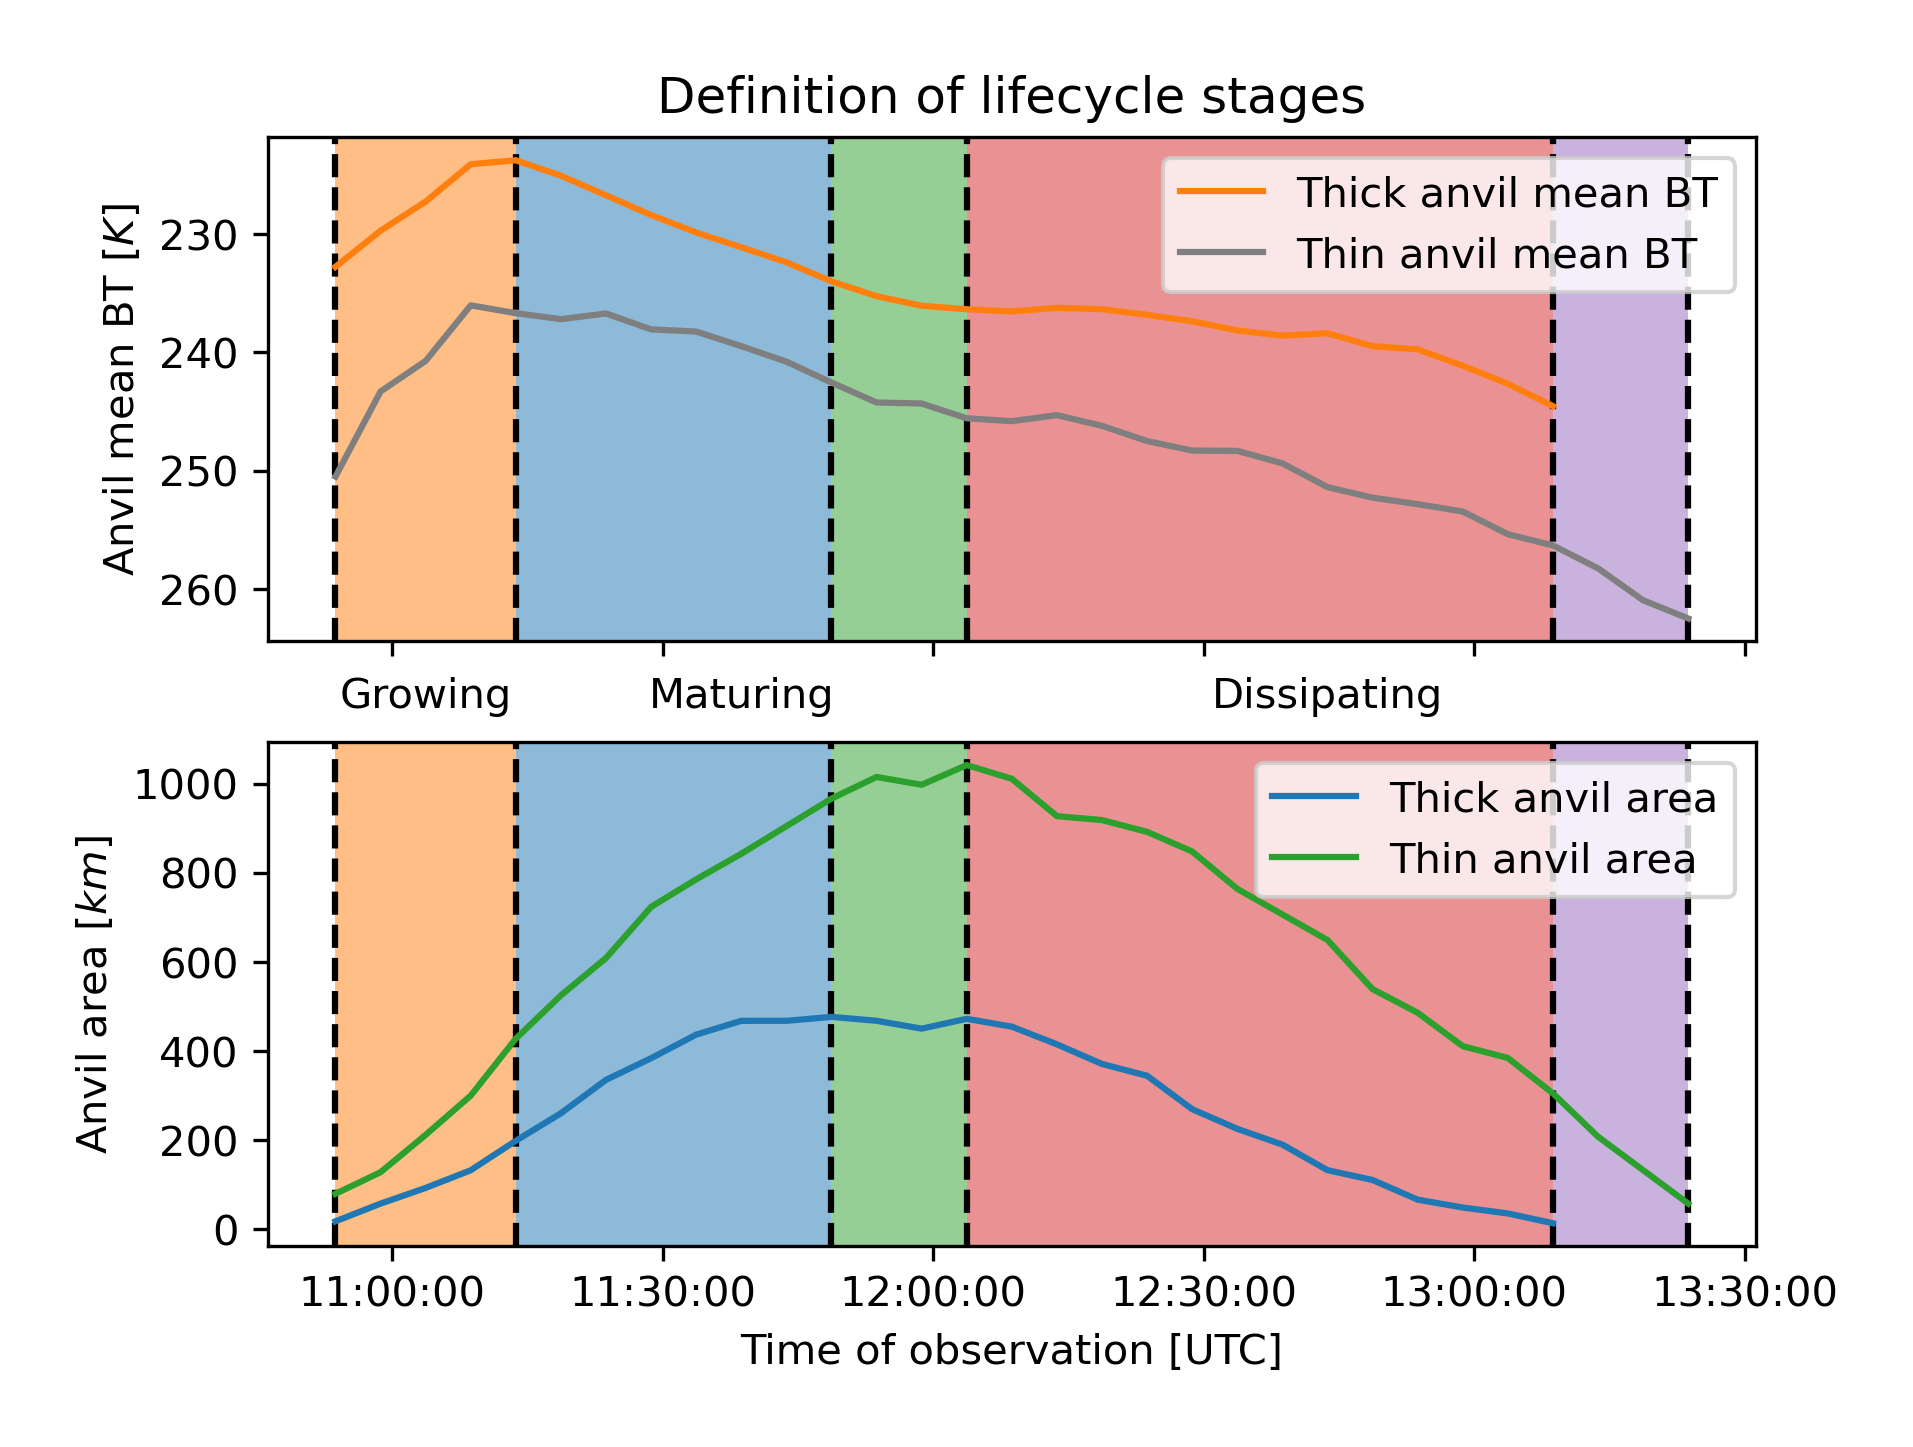
\includegraphics[width=\textwidth]{figures/chapter3_02.png}
    \caption[
    Definition of anvil lifecycle stages based on the method of \citet{futyan_deep_2007}
    ]{
    Definition of anvil lifecycle stages based on the method of \citet{futyan_deep_2007}. The top panel shows the evolution of the mean \acrshort{bt} of the thick and thin anvil regions over the \acrshort{dcc} lifecycle, and the bottom panel shows the evolution of the anvil area. The growing phase (orange) is defined as the time between initial detection and the minimum observed \acrshort{bt}. The mature phase for the thick (blue) and thin (green) anvil is defined as the time between the minimum \acrshort{bt} and maximum thick and thin anvil area respectively. The dissipating phase for the thick (red) and thin (purple) anvils is defined as the time between the anvil maximum area and the final time of detection of the thick and thin anvil respectively.
    }
    \label{fig:lifecycle_example}
\end{figure}

To analyse changes in the lifecycle of \acrshort{dcc}s, their lifetime is categorised based on the method developed by \citet{futyan_deep_2007}.
This method separates the anvil cloud into growing, maturing and dissipating stages based on observations of \acrshort{bt} and anvil area.
\citeauthor{futyan_deep_2007}'s method defines the end of the growing phase as the time at which the anvil reaches its minimum observed \acrshort{bt}, and the end of the mature phase as the time at which the anvil reaches the maximum observed area.
While simple, this approach applies to a wide range of observed \acrshort{dcc}s including both isolated and organised convection.
Furthermore, by determining the anvil lifecycle only in terms of the observed anvil properties, the properties of the detected cores can be treated as independent variables allowing straightforward analysis of their impacts on \acrshort{dcc} lifecycle.

\citeauthor{futyan_deep_2007}'s method is extended in this chapter through consideration of the development of both thick and thin anvil, which results in the lifecycle stages shown in fig.~\ref{fig:lifecycle_example}.
The growing stage (orange) is defined as the time from the initial detection of the \acrshort{dcc} to the time at which the thick anvil has its coldest average \acrshort{bt}.
The thick anvil maturation stage (blue) occurs between this time and the time at which the thick anvil reaches its maximum area, and the thin anvil maturing stage (green) occurs until the thin anvil reaches its maximum area.
In this stage, the thin anvil continues to expand while the thick anvil begins to shrink.
The thick anvil dissipating stage (red) ends at the final detection time of the thick anvil, while the thin anvil dissipating stage (purple) ends at the final detection time of the thin anvil, which is also the final detection time of the tracked \acrshort{dcc}.
By increasing the granularity of the lifecycle definition in this manner, the impact of convective processes on \acrshort{dcc} lifecycle and structure may also be investigated.

\subsection{Composite analysis} \label{sec:composite_definition}

To compare how the structure of tracked \acrshort{dcc} evolves over their lifecycle, the area of their cores, thick and thin anvils is interpolated over a normalised lifetime.
In this normalised lifetime, 0 is defined as the time of initial core detection, and 1 is the time of the final anvil detection.
By normalising their lifetimes in this manner, the change over time of \acrshort{dcc}s with different lifetimes can be composited and compared.


\begin{figure}[tp]
    \centering
    \includegraphics[width=\textwidth]{figures/chapter3_03.png}
    \caption[
    The average evolution of composites of cores (red), thick anvils (orange) and thin anvils (blue) over their normalised lifetimes
    ]{
    The average evolution of composites of cores (red), thick anvils (orange) and thin anvils (blue) over their normalised lifetimes, where 0 is the initial core detection time and 1 is the final anvil detection time. Panel (a) shows the average area of anvils, and (b) shows the proportion of the total area corresponding to each part of the anvil structure.
    }
    \label{fig:composite_example}
\end{figure}

An example composite of the average properties of all analysed anvils in this chapter is shown in fig.~\ref{fig:composite_example}.
Figure~\ref{fig:composite_example}\,a shows the average change in the area of the core (red), thick anvil (orange) and thin anvil (blue) over the normalised lifetime of the \acrshort{dcc}s.
Figure~\ref{fig:composite_example}\,b shows how these areas change as a proportion of the net \acrshort{dcc} area.
This shows how, on average, the structure of \acrshort{dcc}s evolves over their lifetime.
Initially, the \acrshort{dcc} consists entirely of a growing core, with the initial anvil formation occurring between 10\% and 20\% of the \acrshort{dcc} lifetime.
The initial expansion of the anvil is mostly thin, likely because the majority of the mass flux is still travelling upwards, and the area of thick anvil is covered by the developing core.
Between 20\% and 40\% of the normalised lifetime, while the anvil is maturing, the thick and thin anvil expand at similar rates and so the proportion of thin anvil remains consistent.
Beyond this point, the thick anvil reaches its maximum area before the thin anvil and dissipates faster, and the fraction of the thin anvil increases until the end of the \acrshort{dcc} lifecycle.
Note that the average thin anvil fraction does not reach 100\% at the end of the normalised lifetime due to the presence of some \acrshort{dcc}s where the dissipation of the thick and thin anvil are recorded at the same time.

Through the use of composite analysis, the change in anvil structure throughout the \acrshort{dcc} lifecycle can be investigated. 
This allows the study of responses to prior observed convective processes, rather than limiting our analysis to bulk properties or snapshots.

\section{Results}

\subsection{Change in thin anvil fraction with intensity and organisation}

%f
\begin{figure}[tp]
    \centering
    \includegraphics[width=0.75\textwidth]{figures/chapter3_04.png}
    \caption[
    Thin anvil proportion of anvils categorised by mean anvil \acrshort{bt}, initial core cooling rate and number of cores
    ]{
    Thin anvil proportion of anvils categorised by (a) mean anvil \acrshort{bt}, (b) initial core cooling rate, and (c) number of cores. Black error bars show the standard error of the mean, and coloured error bars show the standard deviation.
    }
    \label{fig:thin_anvil_proportion}
\end{figure}

%f
\begin{figure}[tp]
    \centering
    \includegraphics[width=0.75\textwidth]{figures/chapter3_05.png}
    \caption[
    A comparison of the change in thin anvil proportion with maximum core cooling rate and number of cores for four different regions
    ]{
    A comparison of the change in thin anvil proportion with (a) maximum core cooling rate and (b) number of cores for four different regions: sea (blue diamond markers), land (orange square markers), tropics (\textless 30\,\textdegree N; red downward triangle markers) and mid-latitudes (\textgreater 30\,\textdegree N; purple upward triangle markers). Error bars show the standard error of the mean.
    }
    \label{fig:regional_thin_anvil_proportion}
\end{figure}

To begin, the net thin anvil fraction of observed anvils is compared with the mean anvil \acrshort{bt}, initial core maximum cooling rate and number of cores.
Figure~\ref{fig:thin_anvil_proportion}\,a shows how the thin anvil proportion changes with the average thick anvil \acrshort{bt}.
Note that only the thick anvil \acrshort{bt} is considered to avoid a dependence between the anvil \acrshort{bt} and the thin anvil area.
There is an increase of thin anvil proportion with the average anvil \acrshort{bt}, agreeing with the results of \citet{protopapadaki_upper_2017}.
Figure~\ref{fig:thin_anvil_proportion}\,b compares how the thin anvil fraction changes with the maximum cooling rate of the initial core associated with the anvil, and again shows a positive relation between the strength of convection and the thin anvil fraction.
While the value of the thin anvil fraction differs from that observed in previous studies, this is expected as both studies use different methods to define thick and thin.
In addition, in this chapter, the proportion is measured over the entire \acrshort{dcc} lifetime rather than at a single point in time.

In fig.~\ref{fig:thin_anvil_proportion}\,c, the thin anvil fraction is compared to the number of cores associated with each anvil.
In contrast to fig.~\ref{fig:thin_anvil_proportion}\,b and c, there is a decrease in the thin anvil fraction with an increase in the number of cores.
As this occurs despite the tendency for multiple-core anvils to have colder average \acrshort{bt}, this indicates that further factors are involved in the thin anvil fraction than the temperature and height of the anvil.

To ensure that these relationships are not caused by differences in the properties and distributions of \acrshort{dcc}s across different regions, the relationship between cooling rate and number of cores and the thin anvil fraction is further separated into four different regions, shown in fig.~\ref{fig:regional_thin_anvil_proportion}.
As with previous studies, the fraction of thin anvil is very similar for \acrshort{dcc}s observed over land and ocean.
While there is a difference in the thin anvil fraction of approximately 0.05 between \acrshort{dcc}s located in the tropics and mid-latitudes (defined as \textless 30\,\textdegree N and \textgreater 30\,\textdegree N respectively), this difference decreases with increasing convective intensity.
Overall, the near identical relationship of thin anvil fraction to intensity and organisation across multiple regions indicates that this is linked to the convective processes themselves, rather than a co-variance with local conditions.

\subsection{Impact of intensity and organisation on \acrshort{dcc} properties}

Both the intensity and organisation of \acrshort{dcc} cores have impacts on the properties of their anvil clouds.
This section will investigate how these processes affect the bulk properties of these anvils; the anvil maximum area and the anvil lifetime for both thick and thin anvils, and the anvil \acrshort{bt}.
While comparing the bulk properties of these anvils indicates how their structure changes, it does not fully explain the differences shown in figs.~\ref{fig:thin_anvil_proportion} and \ref{fig:regional_thin_anvil_proportion}.

%f
\begin{figure}[tp]
    \centering
    \includegraphics[width=0.75\textwidth]{figures/chapter3_06.png}
    \caption[
    The effect of initial core cooling rate on maximum anvil area, anvil lifetime, and mean and minimum \acrshort{bt}
    ]{
    The effect of initial core cooling rate on (a) maximum anvil area, (b) anvil lifetime, and (c) mean and minimum \acrshort{bt}. Error bars show the standard error of the mean. Points have been staggered to show the thick and thin anvil properties more clearly, but correspond to the same tick marks on the x axis.
    }
    \label{fig:anvil_cooling_rate_properties}
\end{figure}

Figure~\ref{fig:anvil_cooling_rate_properties} shows how the area, lifetime and \acrshort{bt} of \acrshort{dcc}s change with the core cooling rate.
Figure~\ref{fig:anvil_cooling_rate_properties}\,a shows that the average thick and thin anvil maximum areas vary very little with cooling rate, except for at the highest observed values of cooling rate.
There is however a slight widening in the gap between the thick and thin anvil maximum areas with increasing core cooling rate, as the thin anvil increases in maximum area while the thick anvil remains consistent.
Figure~\ref{fig:anvil_cooling_rate_properties}\,b shows that while the average thick anvil lifetime remains constant with increasing core cooling rate, the thin anvil lifetime increases.
There is also a consistent decrease in both average and minimum thick anvil \acrshort{bt} with cooling rate, shown in fig.~\ref{fig:anvil_cooling_rate_properties}\,c.
This change in anvil \acrshort{bt} with the core intensity agrees with the results shown previously in fig.~\ref{fig:core_cooling_rate_relations}\,b which showed that more intense cores have colder minimum \acrshort{bt}.

%f
\begin{figure}[tp]
    \centering
    \includegraphics[width=0.75\textwidth]{figures/chapter3_07.png}
    \caption[
    The effect of the number of cores on maximum anvil area, anvil lifetime, and mean and minimum \acrshort{bt}
    ]{
    The effect of the number of cores on (a) maximum anvil area, (b) anvil lifetime, and (c) mean and minimum \acrshort{bt}. Error bars show the standard error of the mean. Points have been staggered to show the thick and thin anvil properties more clearly, but correspond to the same tick marks on the x axis.
    }
    \label{fig:anvil_number_of_cores_properties}
\end{figure}

In fig.~\ref{fig:anvil_number_of_cores_properties} the change of anvil properties with the number of cores is considered.
Figure~\ref{fig:anvil_number_of_cores_properties}\,a shows that both the thick and thin anvil maximum area increase substantially with an increasing number of cores (note that it is plotted against a log scale).
However, the thin anvil area increases at a slower rate proportional to the thick anvil.
Similarly, there is an increase in both the thick and thin anvil lifetime with increasing number of cores shown in fig.~\ref{fig:anvil_number_of_cores_properties}\,b.
There is a similar rate of the decrease of average anvil \acrshort{bt} with the number of cores in fig.~\ref{fig:anvil_number_of_cores_properties}\,c as shown in relation to core cooling rate in fig.~\ref{fig:anvil_cooling_rate_properties}\,c.
The minimum anvil \acrshort{bt} decreases at a notably faster rate with the increasing number of cores, however.
Although this is indicative of an increased likelihood of overshooting cores in more organised \acrshort{dcc}s, it must also be noted that the larger area of these systems also makes it more likely to observe a colder minimum pixel value.

%f
\begin{figure}[tp]
    \centering
    \includegraphics[width=0.75\textwidth]{figures/chapter3_08.png}
    \caption[
    A comparison of the proportion of thin anvil measured at the time of maximum anvil area, and the proportional difference in lifetime, compared to the overall thin anvil proportion.
    ]{
    A comparison of the proportion of thin anvil measured at the time of maximum anvil area, and the proportional difference in lifetime, compared to the overall thin anvil proportion. Panel (a) shows the change in thin anvil proportion with core cooling rate, and (b) shows the changes with the number of cores. In both panels, the black dotted line shows the total thin anvil proportion over the entire \acrshort{dcc} lifecycle. Error bars show the standard error of the mean of the thin anvil fraction.
    }
    \label{fig:max_area_and_lifetime_contributions}
\end{figure}

The changes in anvil properties with intensity and convection are intriguing due to both their differences and similarities.
Both processes result in anvils with colder \acrshort{bt}, which is commonly used as a proxy for convective intensity.
However, the differences in the changes in anvil areas and lifetimes show that these processes cannot be lumped together so simply.


In fig.~\ref{fig:max_area_and_lifetime_contributions}, the proportion of observed thin anvil fraction that can be attributed to the bulk changes in anvil maximum area and lifetime is shown.
The proportional difference in the maximum area of the thick and thin anvils represents approximately 80\% of the change in thin anvil fraction across both convective intensity and organisation.
This shows that while the trend in thin anvil fraction can be captured by snapshot observations from polar-orbiting satellites, they will underestimate the total thin anvil fraction over the entire \acrshort{dcc} lifetime.
The proportional difference in the thick and thin anvil lifetimes shows a smaller contribution to the net thin anvil fraction.
Furthermore, there is a stronger (positive) trend of the lifetime proportion with intensity and a weaker (negative) trend with organisation.
Note that while some of the error bars (showing the standard deviation) extend below zero, all values for the thin anvil fraction are positive.


\subsection{Changes in \acrshort{dcc} lifecycle with intensity and organisation} \label{sec:lifecycle_results}

It is clear from the impact on anvil lifetime that both the intensity and organisation of convection affect \acrshort{dcc} lifecycle.
Furthermore, fig.~\ref{fig:max_area_and_lifetime_contributions} shows that these different processes have different impacts on the lifecycle that warrant further investigation.
This section will focus on the effect of both convective intensity and organisation on the different lifecycle stages of \acrshort{dcc}s.
The modified \citeauthor{futyan_deep_2007} method explained in section~\ref{sec:lifecycle_definition} is used throughout to separate the anvil lifecycle into growing, mature and dissipating stages.

%f
\begin{figure}[tp]
    \centering
    \includegraphics[width=\textwidth]{figures/chapter3_09.png}
    \caption[
    The average lifetime of each lifecycle stage for anvils categorised by their initial core cooling rate
    ]{
    The lifetime of each of the lifecycle stages, as defined in section~\ref{sec:lifecycle_definition}, for anvils categorised by their initial core cooling rate.
    }
    \label{fig:anvil_cooling_rate_absolute_lifecycle}
\end{figure}

Figure~\ref{fig:anvil_cooling_rate_absolute_lifecycle} shows the lifetime of the different lifecycle stages for \acrshort{dcc}s with increasing core cooling rates.
The lifetime of the growing stage decreases from 1 hour to 45 minutes for the most intense convection.
While these growing lifetimes are longer than those of the detected cores shown in fig.~\ref{fig:core_cooling_rate_relations}, the trend agrees with the shorter lifetime for more intense cores.
Despite the colder \acrshort{bt} and hence higher cloud top heights exhibited by these \acrshort{dcc}s, the stronger vertical growth rates result in an anvil which reaches its minimum \acrshort{bt} in a shorter time frame.

The timing of the maximum extent of the thick anvil remains consistent at just over 1.5 hours for all cooling rates, while the time of the maximum thin anvil area increases from 1 hour 45 minutes to 2 hours for the most intense \acrshort{dcc}s.
Similarly, the timing of the dissipation of the thick remains consistent at just over 3 hours for most cooling rates, while the thin anvil dissipation time increases from 3.5 hours to 4 hours for more intense \acrshort{dcc}s.
These findings reinforce what was shown in fig.~\ref{fig:anvil_cooling_rate_properties}, that the core cooling rate affects the lifetime of the thin anvil but not the thick anvil.

%f
\begin{figure}[tp]
    \centering
    \includegraphics[width=\textwidth]{figures/chapter3_10.png}
    \caption[
    The average fraction of anvil lifetime of each lifecycle stage for anvils categorised by initial core cooling rate
    ]{
    The average fraction of anvil lifetime of each of the lifecycle stages defined in section~\ref{sec:lifecycle_definition} for anvils categorised by initial core cooling rate. Each bar is normalised such that the total length of the row is equal to the mean thin anvil lifetime of its cooling rate bin.
    }
    \label{fig:anvil_cooling_rate_proportional_lifecycle}
\end{figure}

Figure~\ref{fig:anvil_cooling_rate_proportional_lifecycle} displays the average proportion of anvil lifetime spent in each of the stages shown in fig.~\ref{fig:anvil_cooling_rate_absolute_lifecycle}.
The anvil lifetime is normalised using the method described in section~\ref{sec:composite_definition}, where 0 is the time of the initial detection of the \acrshort{dcc} and 1 is the time of the final detection of the dissipating thin anvil.
By analysing these lifecycle stages as a proportion of the total lifetime, better insight is gained into how changes in lifecycle impact the structure and bulk properties of observed \acrshort{dcc}s.

The reduction in the lifetime of the growing phase and increase for thin anvil dissipation for more intense \acrshort{dcc}s is again apparent.
The time between these two stages, representing the period in which the thick anvil matures and then dissipates, lasts for around 60\% of the total anvil lifecycle for all core cooling rates.
The shorter growing period and longer thin anvil dissipating period act together to shift the evolution of the thick anvil earlier in the \acrshort{dcc} lifecycle for more intense \acrshort{dcc}s.
For \acrshort{dcc}s over land, where there is a pronounced peak in occurrence in the afternoon, it is expected that this shifts the time in which the anvil is at its thickest and has the largest extent earlier in the day, potentially increasing its \acrshort{sw} \acrshort{cre}.


%f
\begin{figure}[tp]
    \centering
    \includegraphics[width=\textwidth]{figures/chapter3_11.png}
    \caption[
    The average lifetime of each lifecycle stage for anvils categorised by number of cores
    ]{
    The average lifetime of each of the lifecycle stages defined in section~\ref{sec:lifecycle_definition} for anvils categorised by number of cores.
    }
    \label{fig:anvil_number_of_cores_absolute_lifecycle}
\end{figure}

Figure~\ref{fig:anvil_number_of_cores_absolute_lifecycle} shows how the timing of the different anvil stages changes with increasing number of cores.
It is immediately apparent that the large increase in overall lifetime with the number of cores shown in fig.~\ref{fig:anvil_number_of_cores_properties} also applies to each of the lifecycle stages.
This increase in lifetime occurs to such an extent that the average growing period for \acrshort{dcc}s with 10 or more cores lasts longer than the average of the entire lifetime of isolated \acrshort{dcc}s.
The large spread in lifetimes makes it difficult to compare how the lifecycle changes with organisation without normalising the lifetimes.

%f
\begin{figure}[tp]
    \centering
    \includegraphics[width=\textwidth]{figures/chapter3_12.png}
    \caption[
    The average fraction of anvil lifetime of each lifecycle stage for anvils categorised by number of cores
    ]{
    The average fraction of anvil lifetime of each of the lifecycle stages defined in section~\ref{sec:lifecycle_definition} for anvils categorised by number of cores. Each bar is normalised such that the total length of the row is equal to the mean thin anvil lifetime of its number of cores bin.
    }
    \label{fig:anvil_number_of_cores_proportional_lifecycle}
\end{figure}

Figure~\ref{fig:anvil_number_of_cores_proportional_lifecycle} shows the lifetime of each lifecycle stage as a proportion of the total lifetime for \acrshort{dcc}s with different numbers of cores, in the same manner as used for fig.~\ref{fig:anvil_cooling_rate_proportional_lifecycle}.
In contrast to the effect of increasing intensity, with increasing organisation the length of the growing phase increases and the length of the thin anvil dissipating phase decreases as a proportion of the overall lifetime.
Similar behaviour is seen in the period from the start of the mature phase to the thick anvil dissipation, which remains a consistent length for all core counts.
With increasing organisation, this period shifts later in the lifetime of the \acrshort{dcc}.

It should be clarified, however, that these differences are only in relation to the proportion of total lifetime.
While more organised systems spend a smaller proportion of their lifetime in the thin anvil dissipating phase, the much greater overall lifetime means that this stage still lasts substantially longer than for \acrfull{dcc}s with fewer cores.


\subsection{Changes in thin anvil fraction over \acrshort{dcc} lifecycle} \label{sec:composite_results}

While the contrasting changes in \acrshort{dcc} lifecycle with increasing intensity and organisation (in particular the change in the thin anvil dissipating stage) go some way to explaining the difference in the thin anvil fraction, fig.~\ref{fig:max_area_and_lifetime_contributions} showed that the change in lifetime cannot account for the change in thin anvil fraction alone.
The contrasting changes in lifecycle do, however, indicate that the two convective processes influence how \acrshort{dcc}s evolve over their entire lifetimes.
To further investigate how convective processes impact structure and lifecycle, the composite area approach described in section~\ref{sec:composite_definition} is used to show how the thin anvil fraction evolves over the anvil lifecycle for \acrshort{dcc}s with differing core cooling rates and number of cores.


%f
\begin{figure}[tp]
    \centering
    \includegraphics[width=0.75\textwidth]{figures/chapter3_13.png}
    \caption[
    Mean thin anvil proportion for composites of anvil area of normalised lifetime categorised by the cooling rate of their initial cores.
    ]{
    Mean thin anvil proportion for composites of anvil area of normalised lifetime categorised by the cooling rate of their initial cores. More intense core cooling rates are shown by the darker blue lines.
    }
    \label{fig:cooling_rate_composite}
\end{figure}


Figure~\ref{fig:cooling_rate_composite} shows composites of the thin anvil fraction for \acrshort{dcc}s grouped by core cooling rate, with larger cooling rates shown in darker shades of blue.
Each of the composites has a similar shape to the evolution of thin anvil fraction shown in fig.~\ref{fig:composite_example}\,b; an initial rapid increase as the anvil develops, a plateau during the maturing stage and a continual increase as the anvil dissipates.
Two sections of the lifecycle show divergence in the thin anvil fraction with core cooling rate.
Firstly, more intense cores produce a higher thin anvil fraction during the developing phase.
This difference in thin anvil fraction is then maintained throughout the mature phase.
Secondly, the thin anvil fraction further diverges during the dissipating phase, with the anvils originating from more intense cores having a larger increase in thin anvil fraction.
This difference during the dissipating stage may be related to the difference in the thin anvil lifetime seen previously.


%f
\begin{figure}[tp]
    \centering
    \includegraphics[width=0.75\textwidth]{figures/chapter3_14.png}
    \caption[
    Mean thin anvil proportion for composites of anvil area of normalised lifetime categorised by the number of cores
    ]{
    Mean thin anvil proportion for composites of anvil area of normalised lifetime categorised by the number of cores. Anvils with a larger number of cores are shown by the darker red lines.
    }
    \label{fig:number_of_cores_composite}
\end{figure}

Figure~\ref{fig:number_of_cores_composite} compares how the mean thin anvil fraction changes for composites grouped by the number of cores.
The composites with a greater number of cores are shown by the darker shades of red.
In contrast to fig.~\ref{fig:cooling_rate_composite}, a difference from the typical shape of the thin anvil fraction established in fig.~\ref{fig:composite_example} is seen for more organised \acrshort{dcc}s.
At the end of the initial development phase of the anvil there is a similar thin anvil fraction of around 0.4 across all cases.
While the more organised \acrshort{dcc}s reach this point faster, this is simply due to the initial anvil time making up a smaller proportion of the total lifetime due to the latter's increase with convective organisation.

After the initial development of the anvil, there is a divergence in the thin anvil fraction during the later growing stage and the mature stage.
For the most organised \acrshort{dcc}s, there is a reduction in the thin anvil fraction during this period, indicating that the continuous, organised convection from multiple convective cores leads to a thickening of the anvil.
This difference in thin anvil remains into the dissipating stage, although the composites all converge to a similar fraction by the end of their lifecycles.

The investigation of changes in thin anvil fraction over \acrshort{dcc} lifecycle using composites reveals further complexity to the response of thin anvil structure to convective processes.
Not only do changes in intensity and organisation have contrasting effects on the net thin anvil fraction and the lifecycle, but they also impact the anvil structure at different stages throughout the \acrshort{dcc} lifetime.
The timing of when differences in structure are seen may help investigate the processes through which they occur.


\section{Summary}

Deep convective anvil clouds have a characteristic \acrshort{toa} \acrshort{cre} that is near neutral \citep{hartmann_tropical_2016}.
Anvils are, however, not homogeneous objects, and exhibit structures that transition from thick near the convective cores to thin, detrained cirrus further away.
The tendency of reflectivity to reduce faster than emissivity with reducing cloud optical thickness, combined with the large \acrshort{sw} and \acrshort{lw} \acrshort{cre} of anvils, means that the \acrshort{cre} varies widely with changing thickness \citep{berry_cloud_2014}.
Despite this, the response of anvil optical properties to climate change remains largely uncertain, in part due to the lack of data connecting the behaviour of convective cores and anvils \cite{gasparini_opinion_2023}.

Previous studies have found that the fraction of thin anvil increases with increasing convective intensity \citep{protopapadaki_upper_2017, takahashi_relationships_2017}.
These studies were performed using sun-synchronous polar-orbiting satellite data, and so could not resolve changes across the lifecycle of \acrshort{dcc}s.
With the dataset of tracked \acrshort{dcc} cores and anvils, changes in the convective properties can be related to changes in structure observed over the entire anvil lifecycle.

Using the initial core cooling rate and number of cores as proxies for the intensity and organisation of convection respectively, a similar increase in thin anvil fraction is found with increasing intensity, but a decrease with increasing organisation.
These relationships are found to be robust across a wide range of convective environments.
Contrasting impacts on \acrshort{dcc} lifecycle are also found as a result of both processes.
In more intense \acrshort{dcc}s, there is a reduction in the length of the growing phase and an increase in the thin anvil lifetime, whereas the opposite occurs in more organised cases.
These corresponding changes in lifecycle indicate that the thin anvil fraction cannot be determined from single snapshots alone.

By analysing composites of the change in thin anvil fraction over the \acrshort{dcc} lifecycle, impacts of intensity and organisation are apparent at different periods during the \acrshort{dcc} lifetime.
The timing of these changes also indicates which processes may be impacting the anvil structure in each case.
For the more intense convection, there is an increase in the thin anvil fraction during the initial formation of the anvil, which is then maintained as the anvil matures.
Studies of anvil evolution in high-resolution convective resolving models have shown that, during the initial growth of the anvil, before the development of compensating downdrafts within the core, the divergence of the anvil is directly linked to the updraft velocities within the core \citep{senf_highresolution_2018}.
After the formation of compensating downdrafts after around 15--20 minutes, this connection is broken which may explain why this difference only occurs during the very early formation of the anvil.

A second period of increasing divergence in thin anvil fraction is seen during the dissipating stage of the \acrshort{dcc}s.
As this occurs after the end of the convective updrafts, it cannot be related directly to the convective processes but instead to their impact on the anvil properties.
Over the lifetime of anvils, radiative heating of the cloud base and cooling of the cloud top result in circulations within the anvil cloud which have a thinning effect \citep{gasparini_what_2019}.
Once the anvil is sufficiently thin however (with optical depths around 1), these radiatively driven circulations cease and instead the remainder of the dissipation occurs due to the sedimentation and sublimation of the remaining thin cirrus \citep{sokol_tropical_2020}.
At the higher altitudes and colder temperatures of the anvils produced by more intense convection these processes are substantially slower \citep{seeley_formation_2019}, potentially resulting in larger extents and lifetimes for the thin, but not thick, anvil.

For more organised \acrshort{dcc}s a reduction in the thin anvil fraction is observed not during the initial anvil formation but during the subsequent growing and maturing period of the anvil.
Unlike isolated systems, organised \acrshort{dcc}s involve the continuous development of new convective cores throughout most of the lifecycle of the more organised \acrshort{dcc}s.
It is possible that the thickening is a result of the mesoscale circulations associated with large, organised \acrshort{mcs}s, which transports additional moisture directly into the anvil where it increases the cloud water content at high levels.  
Alternatively, convective aggregation may result in moister environments surrounding the cores of these organised \acrshort{dcc}s, slowing the dissipation of the thick anvil, and also drying the surrounding regions resulting in faster decay of the thin anvil further from the core.
The convergence of the thin anvil fraction during the dissipating phase of \acrshort{dcc}s is indicative of the characteristic decay patterns seen in convective anvils across scales \citep{roca_simple_2017, elsaesser_simple_2022}.

Further investigation of how these processes impact anvil structure and lifecycle may be difficult due to the lack of time-resolved observational data that can measure these processes.
The use of modelling, including both convective resolving models and more idealised experiments, may provide a route to isolate the impacts of each process on \acrshort{dcc} evolution \citep{gasparini_diurnal_2022}.
Lifecycle analysis, as performed in section~\ref{sec:composite_results}, provides opportunities for new constraints on the representation of \acrshort{dcc}s in convective resolving models.
Analysis of km-scale models has revealed responses of anvil structure to changes in convection \citep{sokol_greater_2024}, however as this was performed using bulk analysis it does not provide any insight into the processes which cause this response, or why models differ from each other.
Although geostationary satellite observations cannot observe these processes directly, studying the behaviour of \acrshort{dcc}s over time may provide insight into the relative impacts on different processes.
For example, in fig.~\ref{fig:cooling_rate_composite}, changes in the anvil structure are seen at two points during the convective lifecycle.
Firstly, changes to the anvil during its initial formation must be linked to the convective dynamics themselves, whereas those during the dissipating phase must instead be a result of in situ anvil processes as by this point in the lifecycle the convective dynamics have stopped.
Comparing how anvils in convective resolving models evolve over time to observations may help identify which processes are important to anvil structure and their relative influence, even if these processes cannot be observed themselves.

The final element to consider is how these observed changes in anvil structure may impact the anvil \acrshort{cre}.
Considering the thin anvil fraction alone, it could be expected that more intense \acrshort{dcc}s are more warming due to their thinner structure, and vice versa for more organised convection.
However, this neglects other factors relevant to anvil \acrshort{cre} that are also impacted by convective processes.
Both convective intensity and organisation affect the temperature of anvil clouds, resulting in a warming effect for increases in both.
Furthermore, the observed changes in the lifecycle and the timing of the maximum extent of the thick anvil within the \acrshort{dcc} lifetime may impact the \acrshort{sw} \acrshort{cre}, particularly over land due to the pronounced diurnal cycle of convection.
Observational studies have shown a link between increasing convective organisation and domain mean \acrshort{toa} cooling \citep{bony_observed_2020}.
While this has traditionally been explained as a result of greater clear sky \acrshort{lw} emissions to space \citep{bony_thermodynamic_2016}, this could also result from the response of anvil \acrshort{cre} to changes in structure.

\chapter{The Lifecycle and Cloud Radiative Effect of Deep Convective Clouds Over Africa} \label{chp:radiative_effect}

\section{Introduction}  %% \introduction[modified heading if necessary]
\acrshort{dcc} play a key role in the tropical atmosphere over Africa. 
Forming the ascending branch of the Hadley cells near the equator, \acrshort{dcc}s are critical to the circulation and heat transfer of the tropics \citep{riehl_heat_1958, weisman_mesoscale_2015}. 
The \acrshort{itcz} and its location is vital in determining the seasonal cycles of rainfall over central and western Africa \citep{nicholson_revised_2009, nicholson_itcz_2018}.
Understanding the behaviour of \acrshort{dcc}s over Africa has the potential for major impacts on the atmosphere, weather and society.

% \acrshort{dcc}s are also a cause of extreme weather events including floods, lightning and hail \citep{westra_future_2014}. 
% \acrshort{mcs}s---large, long-lived convective systems in which the anvils of multiple convective cores combine into a single, large `cloud shield' \citep{chen_diurnal_1997, houze_mesoscale_2004, roca_simple_2017}---are responsible for the majority of precipitation in the tropics \citep{feng_global_2021}. 
% 

\acrshort{dcc}s also exert a key influence on the temperature of the tropics through their \acrshort{cre}. 
Due to their size, height and depth, \acrshort{dcc} anvils have large radiative effects in both the \acrshort{sw} and \acrshort{lw}, with both having average magnitudes in excess of 100\,\unit{W m^{-2}} \citep{hartmann_tropical_2016, wall_balanced_2018}. 
Due to the opposite signs of these two components, the average anvil \acrshort{cre} in the tropics is approximately zero \citep{ramanathan_cloud-radiative_1989, hartmann_effect_1992, stephens_cloudsat_2018}. 
Much of the focus on the anvil \acrshort{cre} feedback to global warming has been placed on the \acrshort{lw} response (see section~\ref{sec:anvil_feedbacks}, and in particular only consider the net response of anvils to large scale the tropical atmosphere, rather than the mechanisms affecting individual \acrshort{dcc}s.
In particular, the sensitivity of anvil \acrshort{cre} to changes in the diurnal cycle of convection has recieved little attention.
Previous research has highlighted that changes in the diurnal cycle of convection over Africa may lead to changes in \acrshort{cre} of \textpm 10\,\unit{Wm\textsuperscript{-2}} \citep{nowicki_observations_2004}.
Further investigation into the response of anvil \acrshort{cre} to changes in the diurnal cycle highlighted the need for cloud tracking approaches to study \acrshort{cre} over the anvil lifetime \citep{bouniol_macrophysical_2016, bouniol_life_2021}.


In this chapter, the novel cloud tracking methodology presented in chapter~\ref{chp:tracking_method} is used in conjunction with derived all-sky and clear-sky radiative fluxes to characterise the \acrshort{cre} over the lifecycles of individual anvil clouds. 
This methodology is applied to 4 months of data produced for the \acrshort{esa} Cloud-\acrfull{cci}+ project over sub-Saharan Africa. 
This dataset allows us to investigate both the \acrshort{cre} of individual \acrshort{cre}s, as well as the net anvil \acrshort{cre} over the entire region. 
The overall distribution of anvil \acrshort{cre} is found to be determined by the relationship between \acrshort{dcc} lifecycle and the diurnal cycle of the \acrshort{sw} \acrshort{cre}.
This has important implications for the response of \acrshort{dcc}s to a changing climate, as previously the impact of changes in the diurnal cycle of anvil \acrshort{cre} has seen little study.


\begin{table}[b]
\begin{tabular}{lllcc}
\tophline
Channel & Wavelength (\unit{\mu m}) & Description & Tracking & Retrieval\tabularnewline
\middlehline
1 & 0.64 & Visible & & \checkmark\tabularnewline
2 & 0.81 & \acrshort{nir} & & \checkmark\tabularnewline
3 & 1.64 & \acrshort{nir} & & \checkmark\tabularnewline
4 & 3.92 & \acrshort{nir} Window & & \checkmark\tabularnewline
5 & 6.25 & Upper troposphere \acrshort{wv} & \checkmark & \checkmark\tabularnewline
6 & 7.35 & Lower troposphere \acrshort{wv} & \checkmark & \checkmark\tabularnewline
7 & 8.70 & Mid-IR window & &\tabularnewline
8 & 9.66 & Ozone & &\tabularnewline
9 & 10.8 & Clean \acrshort{lw} window & \checkmark & \checkmark\tabularnewline
10 & 12.0 & Dirty \acrshort{lw} window & \checkmark & \checkmark\tabularnewline
11 & 13.4 & CO\textsubscript{2} & & \checkmark\tabularnewline
12 & 0.6--0.9 & High-resolution visible & &\tabularnewline
\bottomhline
\end{tabular}
% \belowtable{}
\caption{\acrshort{seviri} channels and their use in the \acrshort{dcc} tracking algorithm and cloud properties retrieval.
}
\label{table:seviri_channels}
\end{table}


\section{Data}


For this case study, data is used from \acrshort{seviri} \citep{aminou_msg_2002} aboard the \acrfull{msg} Meteosat-11 satellite, which is in a geostationary orbit above the equator at 0\textdegree W. 
Data from 4 months (May--August 2016) over sub-Saharan Africa (approximately 18\,\textdegree W--46\,\textdegree E, 31\,\textdegree S--15\,\textdegree N) is used at the full resolution of \acrshort{seviri} (3\,\unit{km} at nadir), along with retrieved cloud properties and derived broadband fluxes produced by the \acrshort{esa} Cloud-\acrshort{cci}+ project.
\acrshort{bt} from \acrshort{seviri} is used by the tracking algorithm, and reflectances and \acrshort{bt} are used by the cloud retrieval.

\acrshort{seviri} is a visible and \acrshort{ir} radiometer with a nadir spatial resolution of 3\,\unit{km} and a temporal sampling time of 15 minutes for the full earth disc. 
\acrshort{seviri} has 12 channels across the visible, \acrshort{nir} and thermal-IR spectrum, with one being a high-resolution visible channel with a nadir resolution of 1\,\unit{km}. 
A brief overview of these channels, along with which are used for tracking \acrshort{dcc}s and the cloud properties retrieval, is provided in table~\ref{table:seviri_channels}.


\begin{figure}[tp]
    \includegraphics[width=\textwidth]{figures/chapter4_01.png}
    \caption[
    Example observations from the Meteosat \acrshort{seviri} instrument at 15:00:00 \acrshort{utc} on 2016/6/01
    ]{
    Example observations from the Meteosat \acrshort{seviri} instrument at 15:00:00 \acrshort{utc} on 2016/6/01. a: A visible composite formed using the 1.6, 0.81 and 0.64\,\unit{\mu m} channels as the \acrshort{rgb} channels respectively, with 10.8\,\unit{\mu m} \acrshort{bt} during the night-time. The scene shows a cluster of cold cloud tops (cyan) over central Africa and over the Southern Atlantic. b: 10.8\,\unit{\mu m} \acrshort{bt}. c: \acrshort{wvd} formed by the 6.3\,\unit{\mu m} channel minus the 7.4\,\unit{\mu m} channel. d: \acrshort{swd} formed by the 10.8\,\unit{\mu m} channel minus the 12.0\,\unit{\mu m} channel.
    }
    \label{fig:seviri_obs_example}
\end{figure}

An example of observations from \acrshort{seviri} is shown in fig.~\ref{fig:seviri_obs_example} for 15:00:00~\acrshort{utc} on 1\textsuperscript{st} June 2016. 
A visible composite (fig.~\ref{fig:seviri_obs_example}\,a) is constructed using the 1.64\,\unit{\mu m} and 0.81\,\unit{\mu m} near-infrared and 0.64\,\unit{\mu m} visible channels for the \acrshort{rgb} channels respectively. 
In this composite, ice clouds (which appear cyan) can be seen over central Africa and the southern Atlantic. 
Figure~\ref{fig:seviri_obs_example}\,b shows the 10.8\,\unit{\mu m} brightness temperature for the same scene, showing the coldest temperatures for the high ice clouds over central Africa. 
Two combinations of channels are used for the detection of anvil clouds. 
The \acrshort{wvd}, shown in fig.~\ref{fig:seviri_obs_example}\,c, consists of the 6.3\,\unit{\mu m} \acrshort{bt} minus the 7.4\,\unit{\mu m} \acrshort{bt}. 
The use of these channel combinations for the detection of thick and thin anvil clouds in satellite imagery is detailed in section~\ref{sec:abi_channels}.


\begin{figure}[tp]
    \centering
    \includegraphics[width=0.7\textwidth]{figures/chapter4_06.png}
    \caption[
    Comparison of the sensitivities of \acrshort{abi} (dashed lines) and \acrshort{seviri} (solid lines) to anvil clouds of different optical thickness
    ]{
    Comparison of the sensitivities of \acrshort{abi} (dashed lines) and \acrshort{seviri} (solid lines) to anvil clouds of different optical thickness, using the LibRadTran simulation of an anvil at 14\,\unit{km} as described in section~\ref{sec:theory_anvil}.
    }
    \label{fig:S_abi_seviri_anvil_sensitivity}
\end{figure}



\begin{figure}[tp]
    \centering
    \includegraphics[width=0.75\textwidth]{figures/chapter4_05.png}
    \caption[
    Comparison of the relative spectral response (RSR) functions for the \acrshort{goes}-16 \acrshort{abi} and Meteosat-11 \acrshort{seviri} thermal \acrshort{ir} channels
    ]{
    Comparison of the relative spectral response (RSR) functions for the \acrshort{goes}-16 \acrshort{abi} and Meteosat-11 \acrshort{seviri} thermal \acrshort{ir} channels. The \acrshort{lw} window channels on \acrshort{abi} (channels 13 and 15) have a wider spacing than those of \acrshort{seviri} (channels IR10.8 and IR12.0).}
    \label{fig:S_abi_seviri_rsr}
\end{figure}


Comparing \acrshort{seviri} to \acrshort{abi} (fig.~\ref{fig:S_abi_seviri_anvil_sensitivity}), the 10.8\,\unit{\mu m} \acrshort{bt} (top panel) and \acrshort{wvd} (middle panel) show very similar values for both instruments.
The 10.8\,\unit{\mu m} and 12.0\,\unit{\mu m} channels of \acrshort{seviri} have relatively wide wavebands (see fig.~\ref{fig:S_abi_seviri_rsr}), and as such are less sensitive to the presence of thin ice clouds (fig.~\ref{fig:S_abi_seviri_anvil_sensitivity}\,c), with a response about half that measured by \acrshort{abi}.
Combined with their high \acrshort{nedt} (see table~\ref{table:channel_nedt} and discussion in section~\ref{sec:abi_channels}), it is found that the detection of thin anvil is unreliable using \acrshort{seviri}, and so the thin anvil is not considered within this chapter.



Retrieved cloud properties, including optical thickness, effective radius, liquid/ice water path, \acrshort{ctt} and height, are provided by the \acrfull{cc4cl} algorithm \citep{sus_community_2018, mcgarragh_community_2018}. 
These properties are all retrieved at the same resolution as the input \acrshort{seviri} data. Broadband fluxes are derived using the BUGSRad radiative transfer model \citep{stephens_parameterization_2001} using input cloud properties from the \acrshort{cc4cl} retrieval and vertical temperature, moisture and trace gas profiles from ERA-5 \citep{hersbach_era5_2020}. 
The BUGSRad model provides \acrshort{toa} and \acrlong{boa} \acrshort{lw} and \acrshort{sw} radiative fluxes for both all-sky and clear-sky conditions. An example of these derived fluxes is shown in fig.~\ref{fig:seviri_flux_example}. 
Figure~\ref{fig:seviri_flux_example}\,a shows net \acrshort{toa} fluxes, with a net warming during the daytime on the Western side of the image, and a net cooling at night-time on the Eastern side. 
Figure~\ref{fig:seviri_flux_example}\,b shows the net \acrshort{toa} \acrshort{cre}, with a net cooling effect during the daytime and warming during the night-time for observed high clouds over central Africa. The \acrshort{sw} (fig.~\ref{fig:seviri_flux_example}\,c) and \acrshort{lw} (fig.~\ref{fig:seviri_flux_example}\,d) components of the \acrshort{cre} show that while the \acrshort{lw},
warming component has a smaller magnitude than the day-time, cooling \acrshort{sw} \acrshort{cre}, it remains constant during both day- and night-time.


\begin{figure}[tp]
    \includegraphics[width=\textwidth]{figures/chapter4_02.png}
    \caption[
    An example of the \acrshort{toa} \acrshort{cre} derived using the radiative flux model
    ]{
    An example of the \acrshort{toa} \acrshort{cre} derived using the radiative flux model, for the same time
    as shown in fig.~\ref{fig:seviri_obs_example} (15:00:00 \acrshort{utc} on 2016/6/01). a: net \acrshort{toa} radiative flux. b: net \acrshort{toa} \acrshort{cre}. c: \acrshort{sw} downwards \acrshort{cre}. d: \acrshort{lw} downwards \acrshort{cre}.
    }
    \label{fig:seviri_flux_example}
\end{figure}


\begin{figure}[tp]
    \includegraphics[width=\textwidth]{figures/chapter4_03.png}
    \caption[
    Validation of derived broadband fluxes against monthly \acrshort{ceres}-\acrshort{ebaf} \acrshort{cre}
    ]{
    Validation of derived broadband fluxes against monthly \acrshort{ceres}-\acrshort{ebaf} \acrshort{cre}. a.: The mean difference in net \acrshort{toa} \acrshort{cre} by 1\texttimes 1\textdegree grid square. b.: A comparison of observed \acrshort{toa} net \acrshort{cre} for \acrshort{seviri} against \acrshort{ceres}, with all locations in blue, and those where \acrshort{dcc} anvils are observed in red. c.: the mean difference in \acrshort{sw} \acrshort{toa} \acrshort{cre}. d.: comparison of \acrshort{sw} \acrshort{toa} \acrshort{cre} for \acrshort{seviri} and \acrshort{ceres}. e.: the mean difference in \acrshort{lw} \acrshort{cre}. f.: comparison of \acrshort{lw} \acrshort{toa} \acrshort{cre}. The stippling in a, c and e represents the locations in which \acrshort{dcc} anvils are observed, with the size of the dots corresponding to the number of observations. The solid lines in b, d and f show the linear regression for all locations (blue) and the locations of\acrshort{dcc} anvils (red) weighted by the number of observations.
    }
    \label{fig:flux_validation}
\end{figure}

Validation of the \acrshort{seviri} broadband fluxes was performed against monthly-mean observations of \acrshort{toa} broadband \acrshort{cre} from the \acrfull{ceres} \citep{loeb_clouds_2018} \acrfull{ebaf} climate data record. 
The results of this validation are shown in fig.~\ref{fig:flux_validation}. 
Monthly mean fluxes were calculated for \acrshort{seviri} by first calculating the mean daily fluxes over each 1\texttimes 1\textdegree grid square for days in which over 23 hours of observations are present, and then averaging these daily means over each month. 
Comparison of the net \acrshort{toa} \acrshort{cre} to \acrshort{ceres} revealed a bias of --\,1.87\,\unit{W m\textsuperscript{-2}} (fig.~\ref{fig:flux_validation}\,a,b), consisting of a \acrshort{sw} bias of --\,2.02\,\unit{W m^{-2}} (fig.~\ref{fig:flux_validation}\,c,d) and a \acrshort{lw} bias of $+$\,0.15\,\unit{W m\textsuperscript{-2}} (Fig~\ref{fig:flux_validation}\,e,f). 
Correction for these biases have been applied uniformly to all further \acrshort{cre} values given in this chapter.


\section{Method}


\begin{figure*}[tp]
    \centering
    \includegraphics[width=0.75\textwidth]{figures/chapter4_04.png}
    \caption[
    Simulated sensitivity of the \acrshort{seviri} 10.8\,\unit{\mu m} \acrshort{bt} (top) and \acrshort{wvd} minus \acrshort{swd} (bottom) to anvil clouds of varying optical thickness at heights of 10, 12 and 14\,\unit{km}
    ]{
    Simulated sensitivity of the \acrshort{seviri} 10.8\,\unit{\mu m} \acrshort{bt} (top) and \acrshort{wvd} minus \acrshort{swd} (bottom) to anvil clouds of varying optical thickness at heights of 10, 12 and 14\,\unit{km} as described in section~\ref{sec:theory_anvil}.The grey dashed line shows the 241\,\unit{K} \acrshort{bt}. The grey region in the lower plot shows the range of temperatures in which the edge of the anvil is detected, as described in chapter~\ref{chp:tracking_method}.
    }
    \label{fig:S_anvil_sensitivity}
\end{figure*}

The detection and tracking of \acrshort{dcc}s are performed using the tobac-flow algorithm (see chapter~\ref{chp:tracking_method}, which has been designed specifically to track both isolated and clustered \acrshort{dcc}s in geostationary satellite imagery over their entire lifecycle. 
% While geostationary satellite imagery provides high-resolution observations over large domains and long time periods, which is ideal for studying deep convection, the inability of passive remote sensing to observe convective updrafts directly makes the detection and tracking of \acrshort{dcc}s difficult.

% Algorithms for the detection and tracking of \acrshort{dcc}s in satellite imagery have generally been developed for one of two applications: tracking convective cores and isolated convection, or tracking large \acrshort{mcs} anvils.
% Those designed for tracking deep convective cores, or isolated \acrshort{dcc}s, include Cb-TRAM \citep{zinner_cb-tram_2008,zinner_validation_2013} or tobac \citep{heikenfeld_tobac_2019}.
% These algorithms work by detecting regions of convective updraft or a proxy (such as cloud top cooling rate), and then treating these regions as point-like objects that are advected over time. 
% The second group, designed for tracking \acrshort{mcs}s, include algorithms such as PyFLEXTRKR \citep{feng_pyflextrkr_2022}, TAMS \citep{ocasio_tracking_2020} or TOOCAN \citep{fiolleau_algorithm_2013}. 
% These algorithms detect large regions of cold cloud tops which indicate anvil clouds, and then link them over time by overlapping regions at subsequent time steps. 
% There is no `best' method for tracking all types of convection however \citep{lakshmanan_objective_2010}. 
% The algorithms for tracking isolated convective cells perform worse for clustered convection when the motion and shape of the \acrshort{dcc} cannot be adequately represented as a single vector. 
% On the other hand, the \acrshort{mcs} tracking algorithms perform worse for smaller, isolated \acrshort{dcc}s as the motion of the anvil between time steps may mean it does not overlap with the previous step.

% To approach the challenge of tracking both isolated \acrshort{dcc}s and large, clustered systems, we address the role of cloud motion in the scaling problem. 
% tobac-flow first estimates the motion of \acrshort{dcc}s at each pixel using an optical-flow algorithm. 
% Then, using these estimated motion vectors, we construct a semi-Lagrangian framework in which to perform the detection and tracking. 
% This approach addresses two issues found in traditional cloud tracking approaches.
% First, estimating a motion vector for each pixel allows complex motions (including divergence, rotation, splitting and merging) to be compensated for, rather than just the bulk motion found using the centroid tracking methods.
% Second, by estimating the cloud motion \textit{a priori}, this information can be used within the detection step of the algorithm, and can separate changes in cloud properties such as \acrshort{bt} from those observed due to cloud motion.
% This framework removes the problem of \acrshort{dcc} motion, allowing us to track both isolated and large \acrshort{dcc}s at the same time.

% Three channels and channel combinations from \acrshort{seviri} are used for the detection algorithm: the 10.8\,\unit{\mu m} \acrshort{bt} channel; the \acrshort{wvd} (the difference between the 6.2\,\unit{\mu m} and 7.3\,\unit{\mu m} channels), and the \acrshort{swd} (the difference between the 10.8\,\unit{\mu m} and 12.0\,\unit{\mu m} channels).
% Estimation of cloud motion vectors using optical flow in performed using the 10.8\,\unit{\mu m} \acrshort{bt} channel.
% Detection of cores utilises the 10.8\,\unit{\mu m} \acrshort{bt} channel and the \acrshort{wvd}, and detection of anvils uses \acrshort{wvd} and \acrshort{swd}.

% We detect growing convective cores where we observe regions of rapid cooling in the 10.8\,\unit{\mu m} \acrshort{bt} channel of greater than 0.5\,\unit{Ks\textsuperscript{-1}} and the \acrshort{wvd} of greater than 0.25\,\unit{Ks\textsuperscript{-1}}.
% In both cases
% \acrshort{dcc}s close to the surface and continue tracking them into the upper troposphere. 
% We classify a core as a region of cooling temperature that has existed for at least 15 minutes and has cooled by at least 8\,\unit{K} in a 15-minute period. 
% This threshold provides a strong indicator of intense convective activity \citep{roberts_nowcasting_2003}, and so provides an accurate detection of growing \acrshort{dcc}s.


% Starting from these convective cores, we then detect the surrounding anvil cloud using the \acrshort{wvd} field \citep{muller_role_2018, muller_novel_2019} and continue to detect the anvil until its dissipation, even after the core is no longer visible. 
% A core and anvil are linked with each other if the two overlap at a time when the core has mean \acrshort{wvd} of \textgreater\,5\,\unit{K}, indicating that it has reached the upper troposphere.
% Each anvil cloud can be associated with multiple cores, allowing us to identify cases of clustered convection. 
% As we detect the cores based on cloud-top cooling, however, we can only detect the cores themselves during the growing phase, and cannot detect cores that occur underneath cold, high, anvil clouds.
% When determining the number of cores associated with an anvil, we count the total number of cores observed over the entire lifetime, even if they do not occur at the same time, and including all merges and splits of the anvil cloud.
% This flexibility allows for a wide range of different organised systems to be analysed.


Due to the lack of sensitivity of the \acrshort{seviri} \acrshort{swd} to thin ice clouds, only the thick portion of the anvil is tracked in this chapter.
The \acrshort{wvd} channel of \acrshort{seviri} is capable of detecting anvils with optical thicknesses of approximately 1.5$\pm$0.5 (see fig.~\ref{fig:S_anvil_sensitivity}).
The anvils tracked in this chapter have a median retrieved minimum optical depth of 1.45, although this value may be biased high as many anvils dissipate at night when accurate satellite retrievals of optical depth are not available.
While this sensitivity captures much of the \acrshort{cre} of \acrshort{dcc} anvils \citep{berry_cloud_2014} the long lifetimes of dissipating thin anvils may have a significant warming contribution to net anvil \acrshort{cre} \citep{horner_evolution_2023}.
As a result, it is expected that the anvil \acrshort{cre} measured in this study is biased low.

An example of the cores and anvils detected by the tobac-flow algorithm is shown in fig.~\ref{fig:seviri_detection}, at 3-hour intervals. 
In fig.~\ref{fig:seviri_detection}\,a, a large number of developing cores are seen over central Africa. 
In fig.~\ref{fig:seviri_detection}\,b, there are more developing cores over Western Africa as the pattern of initiation has shifted with westward with the diurnal cycle.
In fig.~\ref{fig:seviri_detection}\,c,d fewer newly developing cores are observed later in the day, but the larger anvil clouds persist into the night-time.


\begin{figure}[tp]
    \includegraphics[width=\textwidth]{figures/chapter4_07.png}
    \caption[
    An example of the cores and anvils (detected by tobac-flow, shown at 3-hour time intervals
    ]{
    An example of the cores (red outline) and anvils (blue outline) detected by tobac-flow plotted over visible composite imagery from \acrshort{seviri}, shown at 3-hour time intervals. All times are given in \acrshort{utc}.
    }
    \label{fig:seviri_detection}
\end{figure}


Over the 4-month period of the case study a total of 145,463 cores (of which 79,592 are associated with anvil clouds) and 35,941 anvils are tracked. 
Using the detected regions of both core and anvil components of tracked \acrshort{dcc}s, the cloud properties and \acrshort{cre} are calculated for each \acrshort{dcc} at each time step from the retrieval and broadband fluxes data. 
The resulting dataset allows us to analyse the properties of each \acrshort{dcc} over their lifetimes from a Lagrangian perspective.
While the studied domain contains both land and sea regions, only a small proportion of tracked \acrshort{dcc}s occurred over sea (11\%), and so analysis of land and oceanic \acrshort{dcc}s are not separated in this chapter.

\section{Results}

\subsection{Spatial and temporal distributions}

Figure~\ref{fig:seviri_map_dists}\,a shows the frequency of core detections for each 1\texttimes 1\textdegree\ grid square over the period of the case study. 
The majority of observed convection occurs over the tropical rainforest regions. 
During the months of May-August, the \acrfull{itcz} is at its northernmost extent over Africa \citep{nicholson_itcz_2018}. 
The West African monsoon occurs during these months, with the primary band of convection located between 5-15\textdegree N \citep{nicholson_revised_2009}, which our observations agree with. 
The maximum frequency of convection is observed at around 6\textdegree N, 12\textdegree E over the Western High Plateau of Cameroon, with high frequencies of convection also observed over the Nigerian coastal plains to the West and the Jos Plateau in Northern Nigeria. 
High rates of convection are also observed over the coastal plains and inland highlands of Guinea, Sierra Leone and Liberia (5--12\,\textdegree N, 5--15\,\textdegree W)
Almost no convective activity is observed between 10\textdegree S and 20\textdegree S as during the Northern hemisphere summer this is the location of the descending branch of the Hadley cell which suppresses convection.


\begin{figure}[tp]
    \includegraphics[width=\textwidth]{figures/chapter4_08.png}
    \caption[
    Number of detected cores and average hour of core detection
    ]{
    a.: The total number of \acrshort{dcc} cores detected over the case study for each 1\texttimes 1\textdegree\ grid box. b.: The average hour of detection for the cores detected in each 1\texttimes 1\textdegree grid box. Grid boxes with a standard deviation greater than 6 hours are single-hatched, and greater than 12 hours cross-hatched.
    }
    \label{fig:seviri_map_dists}
\end{figure}


Figure~\ref{fig:seviri_map_dists}\,b shows the average time of detection for convection in each 1\texttimes 1\textdegree\ grid square. 
The average is calculated as the circular mean of the local solar times of core detection in the grid square. 
Grid squares with a standard deviation greater than 6 hours (indicating a broad spread of initiation times) are given single hatching, and those with standard deviations greater than 12 hours have cross-hatching. 
The most notable feature of the time of detection is the clear contrast between land and sea. 
Convection over the land tends to occur in the afternoon (15:00--18:00), whereas over the ocean it occurs between midnight and early morning (00:00--09:00). 
Furthermore, convection over land tends to occur in a fairly narrow range of times whereas over the ocean convection occurs throughout the diurnal cycle, resulting in the hatching applied to much of the ocean region. 
There is also a noticeable lake effect on the time of convection occurring over Lake Victoria (2\textdegree S, 34\textdegree E) and Lake Tanganyika (7\textdegree S, 31\textdegree E), with convection typically observed in the early morning.

When comparing the regions of Cameroon and Nigeria (4--10\textdegree N, 6--14\textdegree E), where the most growing cores were detected in fig.~\ref{fig:seviri_map_dists}\,a, with the average time of detection in fig.~\ref{fig:seviri_map_dists}\,b, it appears that the grid squares with more cores also tend to have an earlier average time of detection than the surrounding grid squares. 
Precipitation over the Nigerian plains and the Jos Plateau is linked to South-westerly winds bringing moist, warm air from the Gulf of Guinea \citep{vondou_seasonal_2010}. 
This warm air may then trigger convection both through the sea breeze effect and orographic lifting when it reaches the highlands, explaining both the higher frequency and earlier timing of convection compared to surrounding regions. 
A similar relationship between the high frequency of convection and earlier time of detection is also seen over the coastal region and adjacent highlands of Guinea, Sierra Leone and Liberia (5--12\textdegree N, 5--15\textdegree W) which may be due to the same mechanism.

It should be noted that due to the method of detection, cores that develop under existing anvils are less likely to be detected than those in clear sky regions. 
As a result, the occurrence of subsequent developing cores in organised systems may be underestimated, particularly in regions such as the Northern Sahel where a second, night-time peak of precipitation has been observed.

For all further analysis, only cores and anvils that are detected north of 15\textdegree S are considered in order to constrain our analysis to tropical \acrshort{dcc}s.

\subsection{Anvil Cloud Properties}

To investigate how the behaviour of \acrshort{dcc} anvils is affected by their organisation, observed anvils are grouped based on how many cores are associated with them, from isolated \acrshort{dcc}s with one core to highly-clustered \acrshort{dcc}s (such as tropical cloud clusters and \acrshort{mcs}s) with 10 or more cores. 
Anvils with 6--9 cores, and with 10 or more cores, are grouped together to ensure that these groups have a comparable number of members for analysis.

\begin{figure}[tp]
    \includegraphics[width=\textwidth]{figures/chapter4_09.png}
    \caption[
    Anvil statistics by number of associated cores for average maximum area, average lifetime, occurrence of anvils by number of cores, and percentage of total anvil coverage
    ]{
    Anvil statistics by number of associated cores for a.: average maximum area; b.: average lifetime; c.: the number of observed anvils by number of cores; and d.: percentage of total anvil coverage. Error bars in a and b show the standard error of the mean.
    }
    \label{fig:seviri_anvil_stats}
\end{figure}

Figure~\ref{fig:seviri_anvil_stats} shows properties related to the anvil area and lifetime linked to the number of cores. 
In fig.~\ref{fig:seviri_anvil_stats}\,a the average anvil maximum area is shown for each group. 
The maximum area increases approximately linearly with the number of cores, with increasingly clustered anvils having increasingly larger maximum areas, and highly clustered anvils having substantially larger anvils. 
Figure~\ref{fig:seviri_anvil_stats}\,b shows the average anvil lifetime compared to the number of cores. 
While the lifetime also increases with the number of cores, the difference between isolated and highly clustered anvils is proportionately smaller.



Figure~\ref{fig:seviri_anvil_stats}\,c shows the number of anvils observed with differing numbers of cores. 
The vast majority of all anvils observed are isolated \acrshort{dcc}s, with over 80\% having a single detected core. 
As the number of cores increases, the number of anvils detected decreases rapidly. 
However, when considering the large increase in both anvil area and lifetime with the number of cores, the total anvil coverage for highly clustered anvils is much larger (see fig.~\ref{fig:seviri_anvil_stats}\,d). 
Despite their high frequency, isolated \acrshort{dcc}s only account for 12\% of total anvil coverage, whereas highly clustered (10+ cores) account for over 50\%. 
Previous studies have found that despite being few in number, \acrshort{mcs}s account for the majority of precipitation in Western Africa \citep{vizy_understanding_2019}.

\begin{figure}[btp]
    \includegraphics[width=\textwidth]{figures/chapter4_10.png}
    \caption[
    Anvil statistics by number of cores for average anvil \acrshort{ctt} and average minimum anvil temperature
    ]{
    Anvil statistics by number of cores for a.: average anvil \acrshort{ctt}; and b.: average minimum anvil temperature. Error bars show the standard error of the mean.
    }
    \label{fig:seviri_anvil_ctt_stats}
\end{figure}


Figure~\ref{fig:seviri_anvil_ctt_stats}\,a shows the average mean \acrshort{ctt}, and fig.~\ref{fig:seviri_anvil_ctt_stats}\,b the average minimum \acrshort{ctt} for anvils with different numbers of cores. 
While the more clustered anvils have colder average anvil \acrshort{ctt}, this decrease plateaus below 220K indicating that the reduction in clear-sky cooling below this temperature may cap the anvil \acrshort{ctt} for larger \acrshort{dcc}s. 
The minimum observed \acrshort{ctt} within each anvil, however, are colder and show a greater difference with an increasing number of cores. 
The most clustered anvils tend to have a minimum \acrshort{ctt} of around 180\,\unit{K}, indicating the presence of overshooting tops and the most intense convection. 
These cold \acrshort{ctt} values have large uncertainty due to the high sensor noise-to-signal ratio at these cold temperatures.


\begin{figure}[tp]
    \includegraphics[width=\textwidth]{figures/chapter4_11.png}
    \caption[
    The distribution of time to coldest mean anvil \acrshort{ctt}, largest anvil area and time of anvil dissipation
    ]{
    The distribution of time to coldest mean anvil \acrshort{ctt} (orange), largest anvil area (green) and time of anvil dissipation (red) for anvils grouped by number of cores. The vertical lines show the mean time for each distribution.
    }
    \label{fig:seviri_lifetime_dists}
\end{figure}


\citet{futyan_deep_2007} divide the \acrshort{dcc} lifecycle into growing, mature and dissipating phases based on the time of observation of the coldest anvil \acrshort{ctt}, maximum anvil area and dissipation of the anvil. 
Figure~\ref{fig:seviri_lifetime_dists} shows the distribution of the time taken to reach each of these lifecycle milestones for anvils separated by the number of associated cores. 
For all cases, the average time of minimum anvil \acrshort{ctt} occurs before the maximum area, indicating that the anvils continue to grow beyond the maximum of convective activity. 
As the number of cores associated with each anvil increases, the time of the coldest \acrshort{ctt} and largest area occur proportionately earlier during the lifetime of the anvil. 
As a result, these more clustered anvils spend more of their lifetime existing with warming, shrinking anvils than the isolated \acrshort{dcc}s.


\begin{figure}[tp]
    \includegraphics[width=\textwidth]{figures/chapter4_12.png}
    \caption[
    The proportion of anvil lifetime spent in the growing, mature and dissipating phase
    ]{
    The proportion of anvil lifetime spent in the growing (orange), mature (green) and dissipating (red) phase, according to the criteria used by \citet{futyan_deep_2007}
    }
    \label{fig:seviri_lifetime_proportions}
\end{figure}



Figure~\ref{fig:seviri_lifetime_proportions}, compares the proportion of the overall anvil lifetime spent in each of the lifecycle phases defined by \citet{futyan_deep_2007} to the number of cores associated with the anvil. 
There is a clear trend that, as the number of cores increases, the proportion of the lifecycle spent in the growing phase decreases, and the proportion spent in the mature and dissipating phases increases.
Although this approach to classifying the lifecycle of anvil clouds is simplistic and does not capture the complexities of large, long-lived \acrshort{dcc}s which may go through multiple cycles of growth, dissipation and re-invigoration, it provides a useful simplification for comparing complex \acrshort{dcc} lifecycles \citep{roca_simple_2017}. 
The time of the coldest average \acrshort{ctt} will be when the \acrshort{lw} \acrshort{cre} of the anvil cloud is at its greatest, and so can help understand the evolution of the anvil \acrshort{cre} over its lifetime.


\subsection{Anvil \acrshort{cre}}

Using the broadband fluxes data in conjunction with the tracked \acrshort{dcc} dataset enables tracking of how the \acrshort{sw}, \acrshort{lw} and net \acrshort{cre} evolve over the lifetime of each tracked anvil.
Figure~\ref{fig:cre_lifecycle_examples} shows the time series of \acrshort{sw}, \acrshort{lw} and net \acrshort{cre} as well as the cumulative average \acrshort{cre} (the average of net \acrshort{cre} over anvil area and lifetime up until that point in time) for several different anvil lifecycles.
Note that all fluxes are \acrshort{toa} and measured in the downward direction, so a positive value represents warming and a negative value represents cooling.


\begin{figure}[tp]
    \centering
    \includegraphics[width=0.8\textwidth]{figures/chapter4_13.png}
    \caption[
    Anvil net, \acrshort{lw}, and \acrshort{sw} \acrshort{cre}, cumulative mean \acrshort{cre} over anvil lifetime
    ]{
    Anvil net, \acrshort{lw}, and \acrshort{sw} \acrshort{cre}, cumulative mean \acrshort{cre} over anvil lifetime and anvil area for a.: an isolated, short-lived (4-hour) \acrshort{dcc}; b.: a moderately clustered, 1-day long \acrshort{dcc}; and c.: a large, clustered, 4-day long \acrshort{dcc}. All times are the local solar time, to the nearest 5-minute interval. The black lines show the change in area of each \acrshort{dcc} over their lifecycle.
    }
    \label{fig:cre_lifecycle_examples}
\end{figure}


Figure~\ref{fig:cre_lifecycle_examples}\,a shows the case of an isolated, short-lived \acrshort{dcc}. 
The \acrshort{dcc} initiates during the daytime, during which the \acrshort{sw} \acrshort{cre} dominates and the net \acrshort{cre} is negative (cooling). 
However, towards the end of the four-hour lifecycle of the \acrshort{dcc}, it transitions to night-time and so while the \acrshort{sw} \acrshort{cre} reduces and eventually becomes zero, the \acrshort{lw} \acrshort{cre} dominates and the net \acrshort{cre} is positive (warming). 
While this period of warming moves the cumulative average \acrshort{cre} towards zero, it remains overall negative for the overall lifetime of the \acrshort{dcc} both due to the longer period spent during the daytime, and the larger area of the anvil cloud during this period.

Figure~\ref{fig:cre_lifecycle_examples}\,b shows the case of a longer-lived (22 hours), clustered \acrshort{dcc}. 
It initiates in the morning, and so the \acrshort{sw} cooling dominates for the first half of the anvil lifetime. 
Compared to the isolated \acrshort{dcc}, it exists for much longer during the night time, and so the cumulative average becomes positive over the full lifetime of the anvil cloud.

Figure~\ref{fig:cre_lifecycle_examples}\,c shows the case of a four-day, highly clustered convective event. 
In this case, the net \acrshort{cre} alternates between warming and cooling throughout the diurnal cycle. 
The cumulative \acrshort{cre} also alternates between overall warming and cooling throughout the lifetime of the anvil and results in a small net cooling effect.

In both the longer-lived cases (fig.~\ref{fig:cre_lifecycle_examples}\,b, c) the \acrshort{lw} \acrshort{cre} reduces towards the end of the anvil cloud lifetime. 
This may be reflective of the findings from fig.~\ref{fig:seviri_lifetime_dists} that the minimum average \acrshort{ctt} occurs before the mid-point of the cloud lifecycle for longer-lived systems. 
This reduction in \acrshort{lw} \acrshort{cre} may be due to a thinning of the anvil cloud (allowing increased \acrshort{lw} emission from the surface), or due to heating and stabilisation of the upper troposphere by the \acrshort{dcc}.
In addition, the cumulative radiative cooling of the anvil top may drive subsidence and reduce the cloud-top height of the anvil over time \citep{sokol_tropical_2020}.

Figure~\ref{fig:anvil_cre_dist} shows the distribution of net lifetime \acrshort{cre} for all tracked anvils. 
The overall negative average value of --\,0.94\,\textpm\,0.91\,\unit{W m^{-2}} is very close to zero considering the large spread in \acrshort{cre}. 
However, the distribution shows a bimodal structure, with two peaks at around +\,100\,\unit{W m^{-2}} (warming) and --\,180\,\unit{W m^{-2}} (cooling). 
The distribution is coloured according to the mean number of cores associated with the anvils in each bin of the distribution. 
Both the peaks of the distribution are mainly composed of isolated \acrshort{dcc}s which occur during the daytime (negative peak) or night-time (positive peak). 
The centre of the distribution---with average \acrshort{cre}s close to zero---shows a greater number of the clustered \acrshort{dcc}s with multiple cores which, due to their longer lifetime, tend to exist during both the day- and night time.


\begin{figure}[tp]
    \includegraphics[width=\textwidth]{figures/chapter4_14.png}
    \caption[
    The distribution of lifetime anvil \acrshort{cre} for all observed anvils
    ]{
    The distribution of lifetime anvil \acrshort{cre} for all observed anvils. The mean number of cores per anvil in each bin is indicated by the colour scale. The vertical dashed line shows the integrated mean \acrshort{cre} (over area and lifetime) over all anvils, weighted by the anvil areas (--0.94\,\textpm\,0.91\,\unit{W m^{-2}}).
    }
    \label{fig:anvil_cre_dist}
\end{figure}
\begin{figure}[btp]
    \includegraphics[width=\textwidth]{figures/chapter4_15.png}
    \caption[
    The distributions of mean anvil \acrshort{sw} \acrshort{cre} and \acrshort{lw} \acrshort{cre}
    ]{
    The distributions of mean anvil \acrshort{sw} \acrshort{cre} (a) and \acrshort{lw} \acrshort{cre} (b). The vertical dashed line shows the integrated mean \acrshort{cre} over all anvils (\acrshort{sw}: -135.0\,\textpm\,0.9\,\unit{W m^{-2}}, \acrshort{lw}: 134.0\,\textpm\,0.1\,\unit{W m^{-2}})
    }
    \label{fig:anvil_sw_lw_cre}
\end{figure}


In fig.~\ref{fig:anvil_sw_lw_cre} the \acrshort{cre} distribution is broken down into that of the \acrshort{sw} (fig.~\ref{fig:anvil_sw_lw_cre}\,a) and \acrshort{lw} (fig.~\ref{fig:anvil_sw_lw_cre}\,b) components. 
The \acrshort{sw} \acrshort{cre} shows a similar bimodal distribution to that of the net \acrshort{cre}, whereas the \acrshort{lw} distribution shows a normal distribution. 
The \acrshort{sw} \acrshort{cre} has a large peak at 0\,\unit{W m^{-2}} for \acrshort{dcc}s that occur during the night-time, and a broad peak centred around --\,300\,\unit{W m^{-2}} consisting of daytime \acrshort{dcc}s, with the average falling between the two. 
Note that the average for the \acrshort{lw} falls to the right of the peak of the distribution because the average is integrated over the anvil area and lifetime, and the largest and longest-lived anvils tend to have colder \acrshort{ctt} and hence larger \acrshort{lw} \acrshort{cre}.

Figure~\ref{fig:anvil_cre_time_vs_ctt} shows (a) the average instantaneous anvil \acrshort{cre} binned by the time of observation (local solar time) and mean anvil \acrshort{ctt}, and (b) the average lifetime anvil \acrshort{cre} binned by time of initial detection (local solar time) and mean anvil \acrshort{ctt}.
As expected, mean anvil \acrshort{cre} becomes more positive with decreasing \acrshort{ctt} due to increased \acrshort{lw} warming. 
However, the diurnal cycle of detection shows a much stronger contrast, with anvils detected during the daytime having a net cooling effect compared to those at night which have a net warming \acrshort{cre}. 
This diurnal cycle effect is stronger for those anvils with warmer average \acrshort{ctt}, generally representing isolated, shorter-lived \acrshort{dcc}s, and is weaker for colder anvil \acrshort{ctt}. 
Note also that in fig.~\ref{fig:anvil_cre_time_vs_ctt}\,b that the phase of the diurnal cycle shifts to earlier times of detection as average anvil \acrshort{ctt} become colder, as these \acrshort{dcc}s tend to have longer lifetimes.


\begin{figure}[tp]
    \includegraphics[width=\textwidth]{figures/chapter4_16.png}
    \caption[
    Average anvil \acrshort{cre} binned by the time of detection (local time) and mean anvil \acrshort{ctt}
    ]{
    (a) Average instantaneous anvil \acrshort{cre} binned by the time of observation (local solar time) and mean anvil \acrshort{ctt}. (b) Average lifetime anvil \acrshort{cre} binned by time of initial detection (local solar time) and mean anvil \acrshort{ctt}. Hashed regions in (b) show bins in which no anvils were detected.
    }
    \label{fig:anvil_cre_time_vs_ctt}
\end{figure}


It is apparent from figs.~\ref{fig:anvil_cre_dist} and \ref{fig:anvil_sw_lw_cre} that the observed neutral net anvil \acrshort{cre} is not only due to a balance between the \acrshort{sw} and \acrshort{lw}, but also from a balance of the cooling effect of daytime \acrshort{dcc}s and the warming effect of those occurring at night. 
If the number of \acrshort{dcc}s occurring during the daytime were to reduce then there could be a net warming effect without any change to the \acrshort{cre} of individual \acrshort{dcc}s.
As the diurnal cycle of convection over the ocean is nearly uniform, little impact on anvil \acrshort{cre} should be expected from changes in the time of convective initiation.
However, over land, where convective activity is much more common in the afternoon, changes in the diurnal cycle may have a much larger effect on anvil \acrshort{cre}.

Furthermore, fig.~\ref{fig:anvil_cre_time_vs_ctt}\,b highlights that differences in anvil temperature are linked to the diurnal cycle of anvil \acrshort{cre} as colder anvils tend to have longer lifetimes.
As a result, if warming surface temperatures lead to the invigoration of \acrshort{dcc}s, the warming effect would be larger than the \acrshort{lw} effect from the change in anvil temperature alone. 
Surface warming may also result in an earlier time of convective initiation, resulting in a cooling feedback.


\section{Summary}  %% \conclusions[modified heading if necessary]

By combining a novel cloud tracking algorithm with a new dataset of derived all-sky and clear-sky fluxes from geostationary satellite observations, \acrshort{dcc} anvils were detected and tracked along with their associated cores for both isolated and clustered \acrshort{dcc}s, and their properties, lifecycle and \acrshort{cre} investigated. 
As this study was performed using data from May-August (Northern hemisphere summer), the majority of convective activity was observed over the Guinea-Congo rainforest and Savanna regions, as the \acrshort{itcz} is at its northernmost extent.

The degree of convective clustering of each anvil is evaluted by measuring the number of cores it is associated with. 
As expected, anvils with the greatest number of cores---including \acrshort{mcs}s---have larger anvil areas, longer lifetimes and the coldest cloud tops. 
As a result, despite the majority of observed \acrshort{dcc}s being isolated, the highly clustered anvils make up most of the anvil coverage, and so cause most of the anvil impact over this region. 
In addition, the proportion of the lifecycle spent in the mature and dissipating phases increases with the number of cores, and the proportion spent in the growing phase decreases.

When investigating the net \acrshort{cre} of anvils, although the average \acrshort{cre} across all observed anvils is close to zero, few individual anvils have near zero \acrshort{cre} themselves. 
There exists a bimodal distribution of anvil \acrshort{cre}, with isolated \acrshort{dcc}s that exist during the daytime causing the negative (cooling) peak, and those that exist during the night-time causing the positive (warming) peak. 
The systems with near zero \acrshort{cre} tend to live longer with more cores, and exist during both the day- and night-time. 
As a result, when considering the magnitude of the anvil \acrshort{cre}, isolated \acrshort{dcc}s have an outsized contribution to the overall average anvil \acrshort{cre} of 21.4\% compared to their proportion of all anvil coverage (15.3\%) (see fig.~\ref{fig:S_contribution_to_net_cre}).


\begin{figure}[tp]
    \centering
    \includegraphics[width=0.75\textwidth]{figures/chapter4_17.png}
    \caption[
    The contribution to the net CRE for anvils with differing numbers of cores
    ]{
    The contribution to the net CRE for anvils with differing numbers of cores, which is defined as the sum of the absolute CRE multiplied by anvil area for all anvils with that number of cores, divided by the total for all anvils. Due to the large variance and magnitude of the CRE of isolated DCCs, they have a large impact on the net CRE balance despite their small area. 
    }
    \label{fig:S_contribution_to_net_cre}
\end{figure}


The net \acrshort{cre} measured over all anvils (--0.94\,\textpm\,0.91\,\unit{W m^{-2}}) is similarly near zero to many previous studies \citep[][e.g.]{ramanathan_cloud-radiative_1989, hartmann_effect_1992, hartmann_tropical_2016}.
It remains unclear however whether this is an equilibrium state or merely a coincidence.
The role of \acrshort{wv} in the tropical temperature profile, convective dynamics, the height of the convectively active tropopause and the tropical overturning circulation suggests that there may be a link between these factors.
Despite this, no mechanism restoring the tropical anvil \acrshort{cre} to near zero has been discovered.
Whether the anvil \acrshort{cre} should itself be considered near-zero is also debated.
\citet{stephens_cloudsat_2018} argues that, as tropical \acrshort{dcc}s often occur over low-level clouds which have a negative \acrshort{cre} which is cancelled out by the effect of \acrshort{dcc}s, meaning that the near zero \acrshort{toa} \acrshort{cre} is actually a result of a positive anvil \acrshort{cre}.
This line of reasoning has not become more widespread, however.

The interaction between the diurnal cycle of convection and \acrshort{dcc} lifetime plays a key role in the shape of the \acrshort{sw} anvil \acrshort{cre} distribution and is important to consider in regard to anvil \acrshort{cre} feedback. 
As the \acrshort{lw} \acrshort{cre} is normally distributed, a response to changing cloud top height or temperature may occur as a shift in the distribution. 
However, the bimodal distribution of the \acrshort{sw} \acrshort{cre} must result in more complex adjustments to shift the overall mean. 
As the position of the peak at 0 \,\unit{W m^{-2}} relating to night-time \acrshort{dcc}s is fixed, to change the overall average \acrshort{sw} \acrshort{cre} either the width of the distribution has to increase or decrease, or the number of \acrshort{dcc}s occurring during the day- or night-time has to increase. 
The former has important implications for the diurnal cycle of temperature in the tropics, and the latter for the diurnal cycle of convection, which, in turn, affects the anvil lifecycle.

Changes in the diurnal cycle of convection may not have a large impact on net anvil \acrshort{cre} over the ocean due to the mostly uniform occurrence of convection throughout the day.
Over land, however, the afternoon peak of convection at around 3\,pm solar time (see fig.~\ref{fig:seviri_map_dists}) coincides with a time at which anvil \acrshort{cre} is very sensitive to shifts in the diurnal cycle (fig.~\ref{fig:anvil_cre_time_vs_ctt}\,b).
Furthermore, a reduction or increase in the number of \acrshort{dcc}s occurring at a specific time of day may change the net \acrshort{cre} of anvils without any change in the \acrshort{cre} of individual \acrshort{dcc}s.

Diagnosing a diurnal-cycle-related anvil cloud feedback in climate models may however be difficult.
\citet{beydoun_dissecting_2021} found that changes in anvil lifetime contributed little to \acrshort{cre} feedbacks in a cloud-resolving radiative-convective-equilibrium model.
It is unclear how well the diurnal cycle of convection and convective lifecycle are represented in such a model, although convective-resolving models have been found to model these better than parameterised climate models \citep{prein_review_2015, feng_mesoscale_2023}.
Disentangling the impacts of convective processes and anvil cirrus processes on anvil lifecycle and \acrshort{cre} is also a key challenge.
Here, the use of model experiments such as \citet{gasparini_diurnal_2022} may help understand the impacts of each process on anvil \acrfull{cre} and the potential climate feedbacks.

% There are, however, a number of limitations in this study which present opportunities for future research. 
% Firstly, as this study only involved 4 months of data during the Northern Hemisphere summer, the impact of the seasonal cycle on the behaviour of \acrshort{dcc}s and their \acrshort{cre} could not be studied. 
% Furthermore, extending to a larger domain would allow investigation of regional differences, in particular the important land--sea contrast of deep convection \citep{takahashi_revisiting_2023}. 
% A major limitation of the \acrshort{seviri} data is its poor sensitivity to thin anvil cirrus, which has an important impact on net anvil \acrshort{cre} \citep{protopapadaki_upper_2017, horner_evolution_2023}.
% The flexible combined imager \citep{martin_fci_2021} aboard the third-generation Meteosat may allow better detection and study of thin anvil cirrus over tropical Africa in the near future.

% Cloud tracking provides a key capability for the study of deep convective anvil clouds \citep{gasparini_opinion_2023}.
% The ability to observe changes over the lifetime of an anvil cloud independently of changes in the microphysical or macrophysical properties of \acrshort{dcc}s.
% Further application of cloud tracking approaches may better our understanding of \acrshort{dcc} lifecycle, its relation to the diurnal cycle of radiation, and its response to a changing climate.

\chapter{Conclusion} \label{chp:conclusion}

\section{Summary}

\acrshort{dcc}s play a key role in the atmosphere, from extreme weather to the global overturning circulation and energy balance.
Understanding their response to global warming is vital for climate projection, but \acrshort{dcc} feedbacks remain uncertain \citep{sherwood_assessment_2020} and underestimated by current climate models \citep{hill_climate_2023}.
While traditional research on anvil feedbacks has focused on the large scale response of the climate (see section~\ref{sec:anvil_feedbacks}), a spate of novel research has highlighted the importance of convective processes the \acrshort{cre} of anvils \citep{raghuraman_observational_2024, sokol_greater_2024, mckim_weak_2024}.
The mechanisms through which convective processes influence anvil feedbacks remain unclear, in part due to a shortage of observational data connecting the properties of anvils to those of their convective cores \citep{gasparini_opinion_2023}.
With the growing interest in Lagrangian studies of \acrshort{dcc}s \citep{gasparini_what_2019, sokol_tropical_2020, bouniol_life_2021}, there is a need for improved observational constraints on the properties and behaviours of \acrshort{dcc}s.
In this thesis, novel cloud tracking techniques have been applied to geostationary satellite imagery to provide a new perspective on the relationship between convective cores and anvils.

Chapter~\ref{chp:tracking_method} focused on the development of a novel detection and tracking algorithm to better track the behaviour of \acrshort{dcc}s.
\acrshort{dcc} tracking algorithms have been developed for over 60 years, with applications for both weather and climate (see section~\ref{sec:tracking_timeline}).
Despite this, many algorithms still have drawbacks identified decades ago \citep{augustine_mesoscale_1988} that limit their application to developing research areas.
Several key requirements were defined to produce tracking data suitable for studying \acrshort{dcc}s across a wide range of scales and environments.
The algorithm would need to account for both isolated \acrshort{dcc}s and \acrshort{mcs}s, track both convective cores and anvils over the entirety of their lifetimes, and provide estimates of anvil area that are not dependent on other factors such as the anvil height.

Through theory developed using simple, 1D models (section~\ref{sec:detection_theory}), the use of various channel combinations available from modern geostationary imagers was developed to better identify \acrshort{dcc}s in observations.
To avoid the scaling issue between tracking of isolated systems and \acrshort{mcs}s, a semi-Lagrangian scheme was developed that removes the motion dependence from the detection and tracking task.
A detection method for growing convective cores based on cloud top cooling rates was developed, providing a good proxy for the vertical velocity of the core.
In addition, detection methods for both thick and thin anvils were developed using an edge detection scheme.
By avoiding the use of a fixed threshold, this method is more robust to bias than traditional methods, which also enables the detection of anvils both during the mature phase and while dissipating.
Evaluation against lightning observations showed that the combination of core and anvil detection provides a good balance of sensitivity and robustness,  with an F\textsubscript{1}-score of 0.91 providing a high degree of trust in the \acrshort{dcc}s detected by the algorithm.

In chapter~\ref{chp:lifecycle}, this tracking algorithm was applied over five years of geostationary satellite observations from \acrshort{goes}-16 \acrshort{abi}, addressing a key shortage of observational data linking core and anvil properties.
Analysis of this data shows a number of findings including the spatial distribution and land--sea contrasts of deep convection over North America.
Through Lagrangian analysis, the importance of the diurnal cycle both to the properties of \acrshort{dcc}s as well as to other studies could be investigated.
In particular, it was found that due to the contrasting diurnal cycles of convection over land and ocean, the average age of observed anvils varies widely throughout the day.
This contrast is particularly strong in the early afternoon, when \acrshort{dcc}s observed over land tend to be very young while those over the ocean are much older.
As this is the observing time for polar orbiting satellite missions such as those of the \acrshort{atrain}, it was found that snapshot observations from these sensors may find erroneous differences in the properties of \acrshort{dcc}s observed over land and sea due to these contrasting populations at certain times of day.
Combining the capabilities of polar-orbiting sensors with cloud tracking, as performed by \citet{elsaesser_simple_2022}, appears key to addressing these issues.

Previous research has found that the structure of anvil clouds is related to the convective intensity of their cores \citep{protopapadaki_upper_2017, takahashi_relationships_2017}.
In chapter~\ref{chp:anvil_structure}, the response of anvil cloud structure to both their observed intensity and organisation was evaluated using the dataset produced in the previous chapter.
The growing core cooling rate was used as a proxy for convective intensity, and the number of cores as a proxy for organisation, providing more direct proxies than those used in previous studies.
In addition, the thin anvil fraction was evaluated over the entire \acrshort{dcc} lifetime rather than at a single snapshot, capturing the growth and decay of the anvil.

While the relation between convective intensity and thin anvil fraction was found to be similar to that found in previous studies, increases in organisation had an opposing effect on the anvil structure.
The most intense anvils were found to have an increase in the thin anvil fraction of approximately 0.15 over the least intense anvils, whereas the most organised anvils had a fraction 0.12 less than the average for isolated \acrshort{dcc}s.
While convective organisation has a large impact on both the anvil area and lifetime, intensity was found to have little impact on the thick anvil lifetime and area but does increase that of the thin anvil, similar to findings by \citet{sokol_greater_2024}.
Intensity and organisation were also found to have opposing effects on the structure of the \acrshort{dcc} lifecycle.
While increasing intensity shortened the growing phase of the \acrshort{dcc} and lengthened the dissipating phase, organisation had the opposite effect.

To further investigate the cause of these differences, the change in thin anvil fraction over each \acrshort{dcc} lifetime was analysed.
In more intense anvils, differences were found both during the initial stage of anvil formation with more intense updrafts leading to a thinner anvil (indicating a direct impact of convective dynamics on the anvil structure) as well as during the dissipating phase, where the thin anvils produced by more intense \acrshort{dcc}s took longer to dissipate.
For more organised anvils, the main differences were observed during the mature phase of the \acrshort{dcc}, during which time organised systems showed a thickening of the anvil, possibly due to the impact of mesoscale circulations produced by organised convective systems.
While these processes can be observed directly, the use of lifecycle analysis combined with an understanding of how different processes affect \acrshort{dcc}s at different stages of their lifetimes provides insight into what effects these processes may have.
This lifecycle analysis may also be useful in constraining the behaviour of \acrshort{dcc}s in convective resolving models against observations.

 
The novel approach used in this chapter has allowed new results to be found that were not identified in the previous studies.
Explicitly tracking the full lifetime of the anvil cloud results in attributing a larger proportion of thin anvil area than that seen by snapshot observations, and reveals changes caused by an increase in the anvil lifetime.
Furthermore, the explicit tracking of convective cores associated with anvils showed the response of thin anvil area to organisation, whereas without this the trends of organised convection would be hidden due to the majority of observed \acrshort{dcc}s being isolated systems.
In addition, the intensity and organisation of convection are found to have opposing effects on both the lifecycle and structure of \acrshort{dcc}s. 
The thin cirrus produced by \acrshort{dcc}s may have a warming effect on the climate, and so understanding how the area and lifetime of these clouds change with the properties of convection is important to understanding \acrshort{dcc} feedbacks. 
As both the intensity of \acrshort{dcc}s and the frequency of organised convective systems are expected to increase with global warming, so further study of the response of thin cirrus to convective activity is vital.

% \subsection{Chapter~\ref{chp:radiative_effect}: the influence of the diurnal cycle on the \acrshort{cre} of tropical anvil clouds}

Traditionally, considerations of anvil feedbacks have only considered their bulk properties with a present day net anvil \acrshort{cre} of near zero.
In chapter~\ref{chp:radiative_effect}, the cloud tracking method developed in chapter~\ref{chp:tracking_method} is combined with retrieved cloud properties and radiative fluxes from \acrshort{seviri} observations over Africa to investigate how the \acrshort{cre} of individual \acrshort{dcc}s contributes to the net observed \acrshort{cre}. 
Together, this allows us to explicitly measure the \acrshort{cre} of \acrshort{dcc}s over their lifecycle, and analyse how they change with \acrshort{dcc} properties.
The distributions of observed \acrshort{dcc}s show both similarities and differences from those seen in chapter~\ref{chp:lifecycle}.
A similar land--sea contrast was shown in the timing of convective initiation.
This contrast was also seen in the time of initiation over the African Great Lakes (particularly Lake Victoria), which may indicate similar mechanisms in action.
The small number of \acrshort{dcc}s due to the limited extent of the case study prevented further investigation into land--sea contrasts.
The observed \acrshort{dcc} lifecycle, shown in fig.~\ref{fig:seviri_lifetime_proportions}, shows notable differences to those found in chapter~\ref{chp:anvil_structure}, which may have several reasons.
Firstly, there may be a difference in the lifecycle of \acrshort{dcc}s between the tropics and extra-tropics.
However, this difference may have been due to the lower sensitivity of \acrshort{seviri} for observing thin anvils.
This lower sensitivity reduces the length of time over which the anvil is observed, increasing the proportion of the lifecycle observed in the growing phase.
Furthermore, this effect is expected to be greater for isolated \acrshort{dcc}s as the thick anvil dissipates faster than for larger \acrshort{mcs}s.
Finally, the use of retrieved \acrshort{ctt}, rather than observed \acrshort{bt}, may cause a difference.
An increase in stratospheric \acrshort{wv}, along with the thinning of the anvil cloud, will cause the observed \acrshort{bt} of the anvil to increase over time.
However, the retrieved \acrshort{ctt} will remove these effects.
As a result, the method of \citet{futyan_deep_2007} for measuring anvil lifecycle may produce a longer growing phase if \acrshort{ctt} is used instead of \acrshort{bt}.

The main aim of this chapter was the investigation of how the diurnal cycle affects the \acrshort{cre} of individual \acrshort{dcc}s.
Historically, studies into the \acrshort{cre} of tropical anvils have averaged over all areas of anvil cloud without tracking individual \acrshort{dcc}s \citep{ramanathan_cloud-radiative_1989, hartmann_effect_1992, stephens_cloudsat_2018}.
The overall average \acrshort{cre} of our observed \acrshort{dcc}s confirmed the near neutral \acrshort{cre} of tropical anvil clouds with a net value of --0.94\,\textpm\,0.91\,\unit{W m^{-2}}. 
Through the use of tracking, the contribution of individual \acrshort{dcc}s to this mean state and the impact of their properties can be studied.

The \acrshort{cre} of \acrshort{dcc}s changes over their lifetime both due to the changing properties of the anvil cloud and the timing within the diurnal cycle.
While both the \acrshort{lw} and \acrshort{sw} \acrshort{cre} reduce over the lifetime of the \acrshort{dcc}, the \acrshort{sw} \acrshort{cre} is also largely dependent on the time within the diurnal cycle.
These two effects lead to the bimodal distribution for the \acrshort{cre} of individual \acrshort{dcc}s, as shown in fig.~\ref{fig:anvil_cre_dist}.
Three groups of \acrshort{dcc}s are identified that contribute to this distribution.
The largest group is that of isolated \acrshort{dcc}s, which form the two peaks of the distribution.
Typically, these either initiate in the early afternoon and have a negative \acrshort{cre} due to the large \acrshort{sw} effect during the daytime, or initiate in the early evening and instead have a positive \acrshort{cre} as they exist at night.
The second group consists of moderately clustered \acrshort{dcc}s which tend to exist for longer than isolated \acrshort{dcc}s but less than a day.
As these systems tend to initiate in the evening, they mostly exist at night and therefore predominantly have a \acrshort{lw} warming effect.
Finally, \acrshort{mcs}s which exist for multiple days tend to have a neutral \acrshort{cre} as their \acrshort{sw} and \acrshort{lw} effects average out across the diurnal cycle.

The behaviour of these different \acrshort{dcc}s may influence how they respond to climate change.
Organised \acrshort{dcc}s, including \acrshort{mcs}s, may primarily respond through changes in their \acrshort{lw} \acrshort{cre} including \acrshort{fat} and anvil area as \acrshort{sw} changes tend to average out over their lifecycle.
On the other hand, isolated \acrshort{dcc}s tend to have \acrshort{ctt} warmer than the top of the convectively active layer (220\,\unit{K}), and so \acrshort{fat} may not apply to them in the same manner.
The large variance in the \acrshort{cre} of individual isolated \acrshort{dcc}s means that they have a substantially larger influence on the net anvil \acrshort{cre} balance than their area suggests.
As a result, the response of these systems to global warming may have a larger effect on the overall anvil feedback than has been previously considered, and, in particular, they may be sensitive to changes in the diurnal cycle.


\section{Discussion \& Future work}

In recent years there has been an increased focus on the study of anvil lifecycle \citep{wall_life_2018, sokol_tropical_2020} and radiative effects \citep{bouniol_life_2021}.
The response of \acrshort{dcc}s to climate change is both important and uncertain \citep{sherwood_assessment_2020, hill_climate_2023}.
Improving our understanding of cirrus cloud properties and lifecycles is vital to improving this situation \citep{sullivan_ice_2021, gasparini_opinion_2023}.

The key results of this thesis are in the new observational insights into the lifecycle, structure and \acrshort{cre} of \acrshort{dcc}s and their anvils.
The development of a novel tracking algorithm allows both isolated and organised \acrshort{dcc}s to be tracked across their entire lifetime across a wide range of scales.
Furthermore, by tracking both cores and anvil clouds, the behaviours of the convective cores can be linked to the evolution of the anvil clouds, and provide observational evidence for how these properties affect each other.

Chapters~\ref{chp:lifecycle}, and \ref{chp:radiative_effect} showed significant differences in the lifecycles of \acrshort{dcc}s over the land and the ocean.
In particular, these differences may influence \acrshort{dcc} cores and anvils to different extents.
Several processes, occurring over a range of scales, may influence the properties of observed \acrshort{dcc}s.
Lake effects, such as those seen over the African Great Lakes in chapter~\ref{chp:radiative_effect}, may provide a useful case study for understanding these differences, as while their local and surface properties may be similar to that of oceans, the larger environmental conditions may be more affected by the adjacent land regions.

In chapter~\ref{chp:anvil_structure} contrasting impacts of convective intensity and organisation on the structure and lifecycle of anvil clouds were found. 
Analysing how the structure of these \acrshort{dcc}s evolved over their lifetime provided key insights into which convective and anvil processes lead to the observed changes in thick thin anvils.
These contrasts may help further understand the uncertainties in anvil radiative feedbacks, and, in particular, help explain how changes in convection may affect anvil optical properties \citep{mckim_weak_2024}.
In addition, it highlights the importance of isolated \acrshort{dcc}s to the total anvil \acrshort{cre}, motivating further study into how their behaviour differs from organised convection.
Further investigating the contrast between the effects of intensification and organisation on the structure of \acrshort{dcc}s anvils may provide insight into the net changes of anvil structure with climate change. However, while with these structural changes alone, more intense \acrshort{dcc}s are expected to be warming, and more organised \acrshort{dcc}s to be cooling, the changes in \acrshort{bt} and the diurnal cycle observed for both of these processes may dominate any changes in \acrshort{cre}.

A key area of opportunity is in combining the investigation of the impacts of intensity and organisation on anvil structure in chapter~\ref{chp:anvil_structure} with the investigation of anvil \acrshort{cre} in chapter~\ref{chp:radiative_effect}.
While the potential impact of structural changes on anvil \acrshort{cre} was discussed in chapter~\ref{chp:anvil_structure}, explicitly resolving the impact on \acrshort{cre} and comparing it to that due to changes in anvil height and diurnal cycle would advance our understanding of these processes collectively.
To do so, the issues with tracking thin anvils in \acrshort{seviri} observations would need to be overcome.
A larger cloud tracking study, combining these elements, investigating how the microphysical, macrophysical properties and structure of \acrshort{dcc}s change over their lifecycle and throughout the diurnal cycle, and then demonstrating the effect of these changes on the \acrshort{cre} of the anvil across both thick and thin parts and along its entire lifetime, could greatly reduce uncertainties in anvil cloud feedbacks.

\acrshort{dcc}s play a key role in many atmospheric processes, and their response to global warming is both uncertain \citep{sherwood_assessment_2020} and underestimated by current climate models \citep{hill_climate_2023}.
While the new generation of convective resolving models may help to address this problem \citep{stevens_added_2020}, these models still do not fully resolve the issues in simulating the dynamics of deep convection \citep{jeevanjee_vertical_2017} and the behaviour of anvil cirrus \citep{sullivan_ice_2021}.
Observational studies of \acrshort{dcc}s using cloud tracking approaches have been highlighted as a key method to addressing some of these issues \citep{gasparini_opinion_2023}.
In this thesis, we have developed and utilised a novel cloud tracking algorithm to better investigate the properties of \acrshort{dcc} cores and anvils as seen by the latest generation of geostationary weather satellites.
Key results from chapters~\ref{chp:lifecycle}, \ref{chp:anvil_structure} and \ref{chp:radiative_effect} have shown new findings on the properties, structure and \acrshort{cre} of \acrshort{dcc} anvils across their lifecycle, which provide insight into how \acrshort{dcc}s may respond to changes in convective processes and climate change.
The ability to track the properties of \acrshort{dcc}s over their entire lifetimes has been key to these findings.
Understanding the lifecycle of \acrshort{dcc}s from a Lagrangian perspective has been highlighted as a key need for future satellite missions \citep{vandenheever_tropical_2023}, convective resolving model development \citep{prein_kmscale_2024}, and upcoming observation campaigns, and so cloud tracking has a key role to play in future studies of deep convection.


%now enable appendix numbering format and include any appendices
% \appendix
% \chapter{Code availability}

\section{tobac-flow}

\section{tobac}

\section{Thesis}
% \chapter{Data availability}

\section{Thesis data}

\section{CONUS tracking data}

\section{African tracking data}

\section{Satellite data}


\clearpage
\baselineskip=18pt plus1pt

%next line adds the Bibliography to the contents page
\phantomsection
\addcontentsline{toc}{chapter}{Bibliography}
%uncomment next line to change bibliography name to references
%\renewcommand{\bibname}{References}

% \bibliographystyle{jmb.bst}  % bibliography style
\bibliographystyle{apalike}

\begin{small}
\bibliography{bibliography.bib}
\end{small}

\end{document}
